%Page Setup, don't remove
\documentclass[12pt]{book} 
\setlength{\columnsep}{0.7truecm}
\setlength{\parindent}{0cm}
\usepackage[top=2truecm,bottom=2.8truecm, left=2.2truecm, right=2.2truecm,headsep=10pt, paperwidth=19.3truecm, paperheight=27.6truecm]{geometry} 
\usepackage[usenames,dvipsnames]{xcolor}
\usepackage{tcolorbox}
\definecolor{ocre}{RGB}{52,177,201} 
\usepackage{pdfpages}
\usepackage{avant}
\usepackage{bussproofs}
\usepackage{mathptmx}
%\usepackage{ebgaramond}
% \usepackage{xeCJK}
% \setCJKmainfont{SimSun}
\usepackage{tikz}
\usepackage{tkz-euclide}
\usepackage{matchsticks}
\usepackage{wrapfig}
\usepackage{listings}
\usepackage[utf8]{vietnam}
\usepackage{babel}
\usepackage[LSBC5,T1]{fontenc}

%----------------------------------------------------------------------------------------
%	VARIOUS REQUIRED PACKAGES
%----------------------------------------------------------------------------------------
\usepackage{titlesec} % Allows customization of titles
\usepackage{multicol}
\usepackage{graphicx} % Required for including pictures
%\graphicspath{{Pictures/}} % Specifies the directory where pictures are stored
\usepackage{lipsum} % Inserts dummy text
\usepackage{tikz} % Required for drawing custom shapes
%\usepackage{enumitem} % Customize lists
%\setlist{nolistsep} % Reduce spacing between bullet points and numbered lists
\usepackage{booktabs} % Required for nicer horizontal rules in tables
\usepackage{eso-pic} % Required for specifying an image background in the title page
\usepackage{titletoc} % Required for manipulating the table of contents
\contentsmargin{0cm} % Removes the default margin
\usepackage{adjustbox} 
\usepackage{amsmath,amsfonts,amssymb,amsthm} % For math equations, theorems, symbols, etc
%\usepackage[framemethod=tikz]{mdframed} 
\usepackage[sexy]{evan}
\usepackage{hyperref}
\urlstyle{same}
\usepackage{tikz} % figure in two column
\usepackage{float}
\usepackage{biblatex}
\usepackage{caption}% dinh dang figure caption
%\usepackage[font=normalsize]{caption}
\usepackage{changepage}
\usepackage{booktabs}

\usepackage{chngcntr}
\usepackage{array}
\usepackage{eurosym}
\usepackage{multirow}
\usepackage{mathtools}
\usepackage{setspace}
\usepackage{afterpage}
\usepackage{scalerel}
\usepackage{blindtext}
\usepackage{tabularx}
\usepackage{afterpage}
\usepackage{array}
%\usepackage{transparent}
\usepackage{efbox}
\usepackage{tabulary}
% \usepackage{CJKutf8}
\usepackage{subcaption}
\usepackage{rotating}
\usepackage{microtype}
\usepackage{pgfplots}

\usetikzlibrary{lindenmayersystems}
\usetikzlibrary{shapes,shapes.geometric}
\usetikzlibrary{decorations.pathreplacing}
\usetikzlibrary{calc,intersections}
\usetikzlibrary[shadings]
\usetikzlibrary{decorations.fractals}

\newmdenv[skipabove=7pt,
skipbelow=7pt,
backgroundcolor=black!5,
linecolor=ocre,
leftline=true,
innerleftmargin=6pt,
innerrightmargin=6pt,
innertopmargin=8pt,
leftmargin=0cm,
rightmargin=0cm,
innerbottommargin=8pt]{tBox}

\def\PIbox#1{\tikz\node[draw = ocre,fill=black!5,rounded corners,align=justify,text width=.95\linewidth,inner sep=2mm]{#1};}%
\renewcommand{\qedsymbol}{}	
\usepackage{fancyhdr} % Required for header and footer configuration
%%%% Header for duong vao toan hoc
\fancypagestyle{duongvaotoanhoc}{
	\fancyhf{}
	\fancyhead[E]{
		\insertpic{63}{740}{1}{duongvao1}
		\insertpic{333}{35}{1}{fduongvao1}
}
	\fancyhead[O]{
		\insertpic{1}{740}{1}{duongvao2}
		\insertpic{59}{34.9}{1}{fduongvao2}
}	
\renewcommand{\footrulewidth}{0pt}
\fancyfoot[LE,RO]{\sffamily\footnotesize	\thepage}

\fancyfoot[LO,RE]{\sffamily\scriptsize TẬP 6 -- SỐ 10 THÁNG 10/2022}
}

\fancypagestyle{duongvaotoanhocnone}{
	\fancyhf{}
	\fancyhead[E]{
		\insertpic{333}{35}{1}{fduongvao1}
	}
	\fancyhead[O]{
		\insertpic{59}{34.9}{1}{fduongvao2}
	}	
	\renewcommand{\footrulewidth}{0pt}
	\fancyfoot[LE,RO]{\sffamily\footnotesize	\thepage}
	
	\fancyfoot[LO,RE]{\sffamily\scriptsize TẬP 6 -- SỐ 10 THÁNG 10/2022}
}

\fancypagestyle{thachthuctoanhoc}{
	\fancyhf{}
	\fancyhead[E]{
		\insertpic{63}{740}{1}{thachthuc1}
		\insertpic{333}{35}{1}{fthachthuc1}
	}
	\fancyhead[O]{
		\insertpic{1}{740}{1}{thachthuc2}
		\insertpic{59}{34.9}{1}{fthachthuc2}
	}	
	\renewcommand{\footrulewidth}{0pt}
	\fancyfoot[LE,RO]{\sffamily\footnotesize	\thepage}
	
	\fancyfoot[LO,RE]{\sffamily\scriptsize TẬP 6 -- SỐ 10 THÁNG 10/2022}
}

\fancypagestyle{thachthuctoanhocnone}{
	\fancyhf{}
	\fancyhead[E]{
		\insertpic{333}{35}{1}{fthachthuc1}
	}
	\fancyhead[O]{
		\insertpic{59}{34.9}{1}{fthachthuc2}
	}	
	\renewcommand{\footrulewidth}{0pt}
	\fancyfoot[LE,RO]{\sffamily\footnotesize	\thepage}
	
	\fancyfoot[LO,RE]{\sffamily\scriptsize TẬP 6 -- SỐ 10 THÁNG 10/2022}
}


%%%% Header for Toán học và đời sống
\fancypagestyle{toanhocvadoisong}{
			\fancyhf{}
		\fancyhead[E]{
			\insertpic{63}{740}{1}{toanhocds1}
			\insertpic{333}{35}{1}{ftoanhocds1}
		}
		\fancyhead[O]{
			\insertpic{1}{740}{1}{toanhocds2}
			\insertpic{59}{34.9}{1}{ftoanhocds2}
		}	
		\renewcommand{\footrulewidth}{0pt}
		\fancyfoot[LE,RO]{\sffamily\footnotesize	\thepage}
		
		\fancyfoot[LO,RE]{\sffamily\scriptsize TẬP 6 -- SỐ 10 THÁNG 10/2022}
}
\fancypagestyle{toanhocvadoisongnone}{
	\fancyhf{}
	\fancyhead[E]{
		\insertpic{333}{35}{1}{ftoanhocds1}
	}
	\fancyhead[O]{
		\insertpic{59}{34.9}{1}{ftoanhocds2}
	}	
	\renewcommand{\footrulewidth}{0pt}
	\fancyfoot[LE,RO]{\sffamily\footnotesize	\thepage}
	
	\fancyfoot[LO,RE]{\sffamily\scriptsize TẬP 6 -- SỐ 10 THÁNG 10/2022}
}

\fancypagestyle{doisongtoanhoc}{
	\fancyhf{}
	\fancyhead[E]{
		\insertpic{63}{740}{1}{dstoanhoc1}
		\insertpic{333}{35}{1}{fdstoanhoc1}
	}
	\fancyhead[O]{
		\insertpic{1}{740}{1}{dstoanhoc2}
		\insertpic{59}{34.9}{1}{fdstoanhoc2}
	}	
	\renewcommand{\footrulewidth}{0pt}
	\fancyfoot[LE,RO]{\sffamily\footnotesize	\thepage}
	
	\fancyfoot[LO,RE]{\sffamily\scriptsize TẬP 6 -- SỐ 10 THÁNG 10/2022}
}
\fancypagestyle{doisongtoanhocnone}{
	\fancyhf{}
	\fancyhead[E]{
		\insertpic{333}{35}{1}{fdstoanhoc1}
	}
	\fancyhead[O]{
		\insertpic{59}{34.9}{1}{fdstoanhoc2}
	}	
	\renewcommand{\footrulewidth}{0pt}
	\fancyfoot[LE,RO]{\sffamily\footnotesize	\thepage}
	
	\fancyfoot[LO,RE]{\sffamily\scriptsize TẬP 6 -- SỐ 10 THÁNG 10/2022}
}

%%% doi thoai toan hoc
\fancypagestyle{doithoaitoanhoc}{
	\fancyhf{}
	\fancyhead[E]{
		\insertpic{63}{740}{1}{doithoai1}
		\insertpic{333}{35}{1}{fdoithoai1}
	}
	\fancyhead[O]{
		\insertpic{1}{740}{1}{doithoai2}
		\insertpic{59}{34.9}{1}{fdoithoai2}
	}	
	\renewcommand{\footrulewidth}{0pt}
	\fancyfoot[LE,RO]{\sffamily\footnotesize	\thepage}
	
	\fancyfoot[LO,RE]{\sffamily\scriptsize TẬP 6 -- SỐ 10 THÁNG 10/2022}
}
\fancypagestyle{doithoaitoanhocnone}{
	\fancyhf{}
	\fancyhead[E]{
		\insertpic{333}{35}{1}{fdoithoai1}
	}
	\fancyhead[O]{
		\insertpic{59}{34.9}{1}{fdoithoai2}
	}	
	\renewcommand{\footrulewidth}{0pt}
	\fancyfoot[LE,RO]{\sffamily\footnotesize	\thepage}
	
	\fancyfoot[LO,RE]{\sffamily\scriptsize TẬP 6 -- SỐ 10 THÁNG 10/2022}
}

%%%% Header for co dien hien dai
\fancypagestyle{codienhiendai}{
	\fancyhf{}
	\fancyhead[E]{
		\insertpic{63}{740}{1}{codien1}
		\insertpic{333}{35}{1}{fcodien1}
	}
	\fancyhead[O]{
		\insertpic{1}{740}{1}{codien2}
		\insertpic{59}{34.9}{1}{fcodien2}
	}	
	\renewcommand{\footrulewidth}{0pt}
	\fancyfoot[LE,RO]{\sffamily\footnotesize	\thepage}
	
	\fancyfoot[LO,RE]{\sffamily\scriptsize TẬP 6 -- SỐ 10 THÁNG 10/2022}
}
\fancypagestyle{codienhiendainone}{
	\fancyhf{}
	\fancyhead[E]{
		\insertpic{333}{35}{1}{fcodien1}
	}
	\fancyhead[O]{
		\insertpic{59}{34.9}{1}{fcodien2}
	}	
	\renewcommand{\footrulewidth}{0pt}
	\fancyfoot[LE,RO]{\sffamily\footnotesize	\thepage}
	
	\fancyfoot[LO,RE]{\sffamily\scriptsize TẬP 6 -- SỐ 10 THÁNG 10/2022}
}

\fancypagestyle{diendandayvahoctoan}{
	\fancyhf{}
	\fancyhead[E]{
		\insertpic{63}{740}{1}{diendan1}
		\insertpic{333}{35}{1}{fdiendan1}
	}
	\fancyhead[O]{
		\insertpic{1}{740}{1}{diendan2}
		\insertpic{59}{34.9}{1}{fdiendan2}
	}	
	\renewcommand{\footrulewidth}{0pt}
	\fancyfoot[LE,RO]{\sffamily\footnotesize	\thepage}
	
	\fancyfoot[LO,RE]{\sffamily\scriptsize TẬP 6 -- SỐ 10 THÁNG 10/2022}
}
\fancypagestyle{diendandayvahoctoannone}{
	\fancyhf{}
	\fancyhead[E]{
		\insertpic{333}{35}{1}{fdiendan1}
	}
	\fancyhead[O]{
		\insertpic{59}{34.9}{1}{fdiendan2}
	}	
	\renewcommand{\footrulewidth}{0pt}
	\fancyfoot[LE,RO]{\sffamily\footnotesize	\thepage}
	
	\fancyfoot[LO,RE]{\sffamily\scriptsize TẬP 6 -- SỐ 10 THÁNG 10/2022}
}

\fancypagestyle{cackithitoan}{
	\fancyhf{}
	\fancyhead[E]{
		\insertpic{63}{740}{1}{cackithi1}
		\insertpic{333}{35}{1}{fcackithi1}
	}
	\fancyhead[O]{
		\insertpic{1}{740}{1}{cackithi2}
		\insertpic{59}{34.9}{1}{fcackithi2}
	}	
	\renewcommand{\footrulewidth}{0pt}
	\fancyfoot[LE,RO]{\sffamily\footnotesize	\thepage}
	
	\fancyfoot[LO,RE]{\sffamily\scriptsize TẬP 6 -- SỐ 10 THÁNG 10/2022}
}
\fancypagestyle{cackithitoannone}{
	\fancyhf{}
	\fancyhead[E]{
		\insertpic{333}{35}{1}{fcackithi1}
	}
	\fancyhead[O]{
		\insertpic{59}{34.9}{1}{fcackithi2}
	}	
	\renewcommand{\footrulewidth}{0pt}
	\fancyfoot[LE,RO]{\sffamily\footnotesize	\thepage}
	
	\fancyfoot[LO,RE]{\sffamily\scriptsize TẬP 6 -- SỐ 10 THÁNG 10/2022}
}

\fancypagestyle{lichsutoanhoc}{
	\fancyhf{}
	\fancyhead[E]{
		\insertpic{63}{740}{1}{lichsu1}
		\insertpic{333}{35}{1}{flichsu1}
	}
	\fancyhead[O]{
		\insertpic{1}{740}{1}{lichsu2}
		\insertpic{59}{34.9}{1}{flichsu2}
	}	
	\renewcommand{\footrulewidth}{0pt}
	\fancyfoot[LE,RO]{\sffamily\footnotesize	\thepage}
	
	\fancyfoot[LO,RE]{\sffamily\scriptsize TẬP 6 -- SỐ 10 THÁNG 10/2022}
}
\fancypagestyle{lichsutoanhocnone}{
	\fancyhf{}
	\fancyhead[E]{
		\insertpic{333}{35}{1}{flichsu1}
	}
	\fancyhead[O]{
		\insertpic{59}{34.9}{1}{flichsu2}
	}	
	\renewcommand{\footrulewidth}{0pt}
	\fancyfoot[LE,RO]{\sffamily\footnotesize	\thepage}
	
	\fancyfoot[LO,RE]{\sffamily\scriptsize TẬP 6 -- SỐ 10 THÁNG 10/2022}
}

%%%% Header for Tìm hiểu khoa học
\fancypagestyle{timhieukhoahoc}{
		\fancyhf{}
	\fancyhead[E]{
		\insertpic{63}{740}{1}{timhieu1}
		\insertpic{333}{35}{1}{ftimhieu1}
	}
	\fancyhead[O]{
		\insertpic{1}{740}{1}{timhieu2}
		\insertpic{59}{34.9}{1}{ftimhieu2}
	}	
	\renewcommand{\footrulewidth}{0pt}
	\fancyfoot[LE,RO]{\sffamily\footnotesize	\thepage}
	
	\fancyfoot[LO,RE]{\sffamily\scriptsize TẬP 6 -- SỐ 10 THÁNG 10/2022}	
}
\fancypagestyle{timhieukhoahocnone}{
	\fancyhf{}
	\fancyhead[E]{
		\insertpic{333}{35}{1}{ftimhieu1}
	}
	\fancyhead[O]{
		\insertpic{59}{34.9}{1}{ftimhieu2}
	}	
	\renewcommand{\footrulewidth}{0pt}
	\fancyfoot[LE,RO]{\sffamily\footnotesize	\thepage}
	
	\fancyfoot[LO,RE]{\sffamily\scriptsize TẬP 6 -- SỐ 10 THÁNG 10/2022}	
}

%%%% Header for quan toan
\fancypagestyle{quantoan}{
		\fancyhf{}
		\fancyhead[E]{
		\insertpic{63}{740}{1}{quantoan1}
		\insertpic{333}{35}{1}{fquantoan1}
	}
	\fancyhead[O]{
		\insertpic{1}{740}{1}{quantoan2}
		\insertpic{59}{34.9}{1}{fquantoan2}
	}	
	\renewcommand{\footrulewidth}{0pt}
	\fancyfoot[LE,RO]{\sffamily\footnotesize	\thepage}
	
	\fancyfoot[LO,RE]{\sffamily\scriptsize TẬP 6 -- SỐ 10 THÁNG 10/2022}
}
\fancypagestyle{quantoannone}{
	\fancyhf{}
	\fancyhead[E]{
		\insertpic{333}{35}{1}{fquantoan1}
	}
	\fancyhead[O]{
		\insertpic{59}{34.9}{1}{fquantoan2}
	}	
	\renewcommand{\footrulewidth}{0pt}
	\fancyfoot[LE,RO]{\sffamily\footnotesize	\thepage}
	
	\fancyfoot[LO,RE]{\sffamily\scriptsize TẬP 6 -- SỐ 10 THÁNG 10/2022}
}


\fancypagestyle{hoccungpi}{
				\fancyhf{}
		\fancyhead[E]{
			\insertpic{63}{740}{1}{hoccungpi1}
			\insertpic{333}{35}{1}{fhoccungpi1}
		}
		\fancyhead[O]{
			\insertpic{1}{740}{1}{hoccungpi2}
			\insertpic{59}{34.9}{1}{fhoccungpi2}
		}	
		\renewcommand{\footrulewidth}{0pt}
		\fancyfoot[LE,RO]{\sffamily\footnotesize	\thepage}
		
		\fancyfoot[LO,RE]{\sffamily\scriptsize TẬP 6 -- SỐ 10 THÁNG 10/2022}	
}
\fancypagestyle{hoccungpinone}{
	\fancyhf{}
	\fancyhead[E]{
		\insertpic{333}{35}{1}{fhoccungpi1}
	}
	\fancyhead[O]{
		\insertpic{59}{34.9}{1}{fhoccungpi2}
	}	
	\renewcommand{\footrulewidth}{0pt}
	\fancyfoot[LE,RO]{\sffamily\footnotesize	\thepage}
	
	\fancyfoot[LO,RE]{\sffamily\scriptsize TẬP 6 -- SỐ 10 THÁNG 10/2022}	
}

\fancypagestyle{toancuabi}{
	\fancyhf{}
	\fancyhead[E]{
		\insertpic{63}{740}{1}{toancuabi1}
		\insertpic{333}{35}{1}{ftoancuabi1}
	}
	\fancyhead[O]{
		\insertpic{1}{740}{1}{toancuabi2}
		\insertpic{59}{34.9}{1}{ftoancuabi2}
	}	
	\renewcommand{\footrulewidth}{0pt}
	\fancyfoot[LE,RO]{\sffamily\footnotesize	\thepage}
	
	\fancyfoot[LO,RE]{\sffamily\scriptsize TẬP 6 -- SỐ 10 THÁNG 10/2022}	
}
\fancypagestyle{toancuabinone}{
	\fancyhf{}
	\fancyhead[E]{
		\insertpic{333}{35}{1}{ftoancuabi1}
	}
	\fancyhead[O]{
		\insertpic{59}{34.9}{1}{ftoancuabi2}
	}	
	\renewcommand{\footrulewidth}{0pt}
	\fancyfoot[LE,RO]{\sffamily\footnotesize	\thepage}
	
	\fancyfoot[LO,RE]{\sffamily\scriptsize TẬP 6 -- SỐ 10 THÁNG 10/2022}	
}

\fancypagestyle{gocco}{
	\fancyhf{}
	\fancyhead[E]{
		\insertpic{63}{740}{1}{gocco1}
		\insertpic{333}{35}{1}{fgocco1}
	}
	\fancyhead[O]{
		\insertpic{1}{740}{1}{gocco2}
		\insertpic{59}{34.9}{1}{fgocco2}
	}	
	\renewcommand{\footrulewidth}{0pt}
	\fancyfoot[LE,RO]{\sffamily\footnotesize	\thepage}
	
	\fancyfoot[LO,RE]{\sffamily\scriptsize TẬP 6 -- SỐ 10 THÁNG 10/2022}	
}

\fancypagestyle{gocconone}{
	\fancyhf{}
	\fancyhead[E]{
		\insertpic{333}{35}{1}{fgocco1}
	}
	\fancyhead[O]{
		\insertpic{59}{34.9}{1}{fgocco2}
	}	
	\renewcommand{\footrulewidth}{0pt}
	\fancyfoot[LE,RO]{\sffamily\footnotesize	\thepage}
	
	\fancyfoot[LO,RE]{\sffamily\scriptsize TẬP 6 -- SỐ 10 THÁNG 10/2022}	
}
	
%	\fancyfoot[C]{\sffamily\footnotesize Tạp chí Pi } % Print the nearest section name on the left side of odd pages	


\pagestyle{fancy}
\renewcommand{\chaptermark}[1]{\markboth{\normalsize\bfseries\chaptername\ \thechapter.\ #1}{}} % Chapter text font settings
\renewcommand{\sectionmark}[1]{\markright{\normalsize\thesection\hspace{5pt}#1}{}} % Section text font settings


\fancyfoot[LE,RO]{\sffamily\footnotesize	\thepage} % Font setting for the page number in the header
\fancyfoot[LO,RE]{\sffamily\footnotesize TẬP 6 -- SỐ 10 THÁNG 10/2022 \LARGE  $\pmb{\pi}$}


\fancyfoot[C]{\sffamily\footnotesize Tạp chí Pi } % Print the nearest section name on the left side of odd pages
\renewcommand{\headrulewidth}{0pt} % Width of the rule under the header
\addtolength{\headheight}{2.5pt} % Increase the spacing around the header slightly
\renewcommand{\footrulewidth}{.5pt} % Removes the rule in the footer


\fancypagestyle{plain}{\fancyhead{}\renewcommand{\headrulewidth}{0pt}} % Style for when a plain pagestyle is specified

% Removes the header from odd empty pages at the end of chapters
\makeatletter
\renewcommand{\cleardoublepage}{
	\clearpage\ifodd\c@page\else
	\hbox{}
	\vspace*{\fill}
	\thispagestyle{empty}
	\newpage
	\fi}


\graphicspath{{../main/pic/}}
\everymath{\displaystyle}
\DeclareMathAlphabet{\pazocal}{OMS}{zplm}{m}{n}
\usepackage{ebgaramond}
\usepackage{xpatch}
\PassOptionsToPackage{hyphens}{url}

\usepackage{url}
\usepackage{type1cm}
\usepackage{lettrine}
\usepackage{makecell}
\renewcommand{\LettrineTextFont}{\rmfamily}
\usepackage{skak}
%\usepackage{xskak}
\usepackage{tabularx}
\usepackage{microtype}
\usepackage{cases}
\usepackage{tikz-cd}
\usepackage{oplotsymbl}
\definecolor{codienhiendai}{cmyk}{0.72, 0, 0.42, 0.1}
\definecolor{thachthuctoanhoc}{cmyk}{0.87, 0.46, 0.69, 0.31}
\definecolor{diendantoanhoc}{cmyk}{0.75, 0, 0.7, 0}
\definecolor{timhieukhoahoc}{cmyk}{0.84, 0.7, 0, 0}
\definecolor{quantoan}{cmyk}{0.8, 0.57, 0, 0}
\definecolor{cackithi}{cmyk}{0.7, 0.35, 0, 0}
\definecolor{hoccungpi}{cmyk}{0.67, 0.6, 0, 0}
\definecolor{gocco}{cmyk}{0.65, 0.78, 0, 0}
\definecolor{toancuabi}{cmyk}{0, 1, 0, 0}
\definecolor{doithoaitoanhoc}{cmyk}{0.6, 0.3, 0 ,0.63}
\definecolor{duongvaotoanhoc}{cmyk}{0, 0.7, 0.9, 0}
\definecolor{toanhocdoisong}{cmyk}{0 , 0.93, 1, 0}
\definecolor{tramthienvan}{cmyk}{0, 0.98, 0.95, 0}
\definecolor{lichsutoanhoc}{cmyk}{0.35, 0.5, 0.8, 0.1}
\definecolor{doisongtoanhoc}{cmyk}{0.25, 0.3, 0.5, 0.1}
\definecolor{amber}{rgb}{1.0, 0.75, 0.0}

\definecolor{darkblue}{rgb}{0.089,0.21,0.363}
\usepackage[hang,splitrule]{footmisc}
\usetikzlibrary{arrows}
\usetikzlibrary{patterns}
\usetikzlibrary{decorations.pathreplacing,calligraphy,backgrounds}
\setlength{\footnotemargin}{0cm}
\setlength{\footnotesep}{0.35cm}
\setlength{\skip\footins}{0.35cm}
\setlength\footskip{33pt}

\newcommand\blfootnote[1]{%
	\begingroup
	\renewcommand\thefootnote{}\footnote{#1}%
	\addtocounter{footnote}{-1}%
	\endgroup
}

\def\footnotelayout{\itshape}
\renewcommand*\footnoterule{}
\renewcommand\footnoterule{\vspace*{0.25cm}\hrule width 1\textwidth\vspace*{0.25cm}}

\newcommand{\insertpic}[4]{
	\begingroup
	\AddToShipoutPicture*{\put(#1,#2){\includegraphics[scale=#3]{#4}}} % %Image background
	\centering
	\endgroup
}

\tikzset{
	squarednode/.style={rectangle, draw=red!60, fill=red!5, very thick, minimum size=3mm}
}

\tikzset{
	sqnode/.style={rectangle, draw=cackithi, very thick, minimum size=3mm}
}

\tikzset{
	roundnode/.style={circle, draw=toancuabi, fill=cackithi!50, minimum size=3mm},
}


\begin{document}
%	 \thispagestyle{empty}
%	 \begingroup 
%	 \AddToShipoutPicture*{\put(0,0){\includegraphics[scale=1]{ML.pdf}}}
%	 \centering
%	 \vspace*{0cm}
%	 \endgroup
%	 \newpage	  
%	 \pagestyle{empty}
%
%	\setcounter{page}{2}
%
%	\setcounter{figure}{0}
%	\thispagestyle{toanhocvadoisongnone}
\pagestyle{toanhocvadoisong}
\everymath{\color{toanhocdoisong}}
\graphicspath{{../toanhocdoisong/pic/}}
\begingroup
\blfootnote{$^1$\color{toanhocdoisong}Viện Sinh thái và Môi trường Đông Dương.}
\AddToShipoutPicture*{\put(0,616){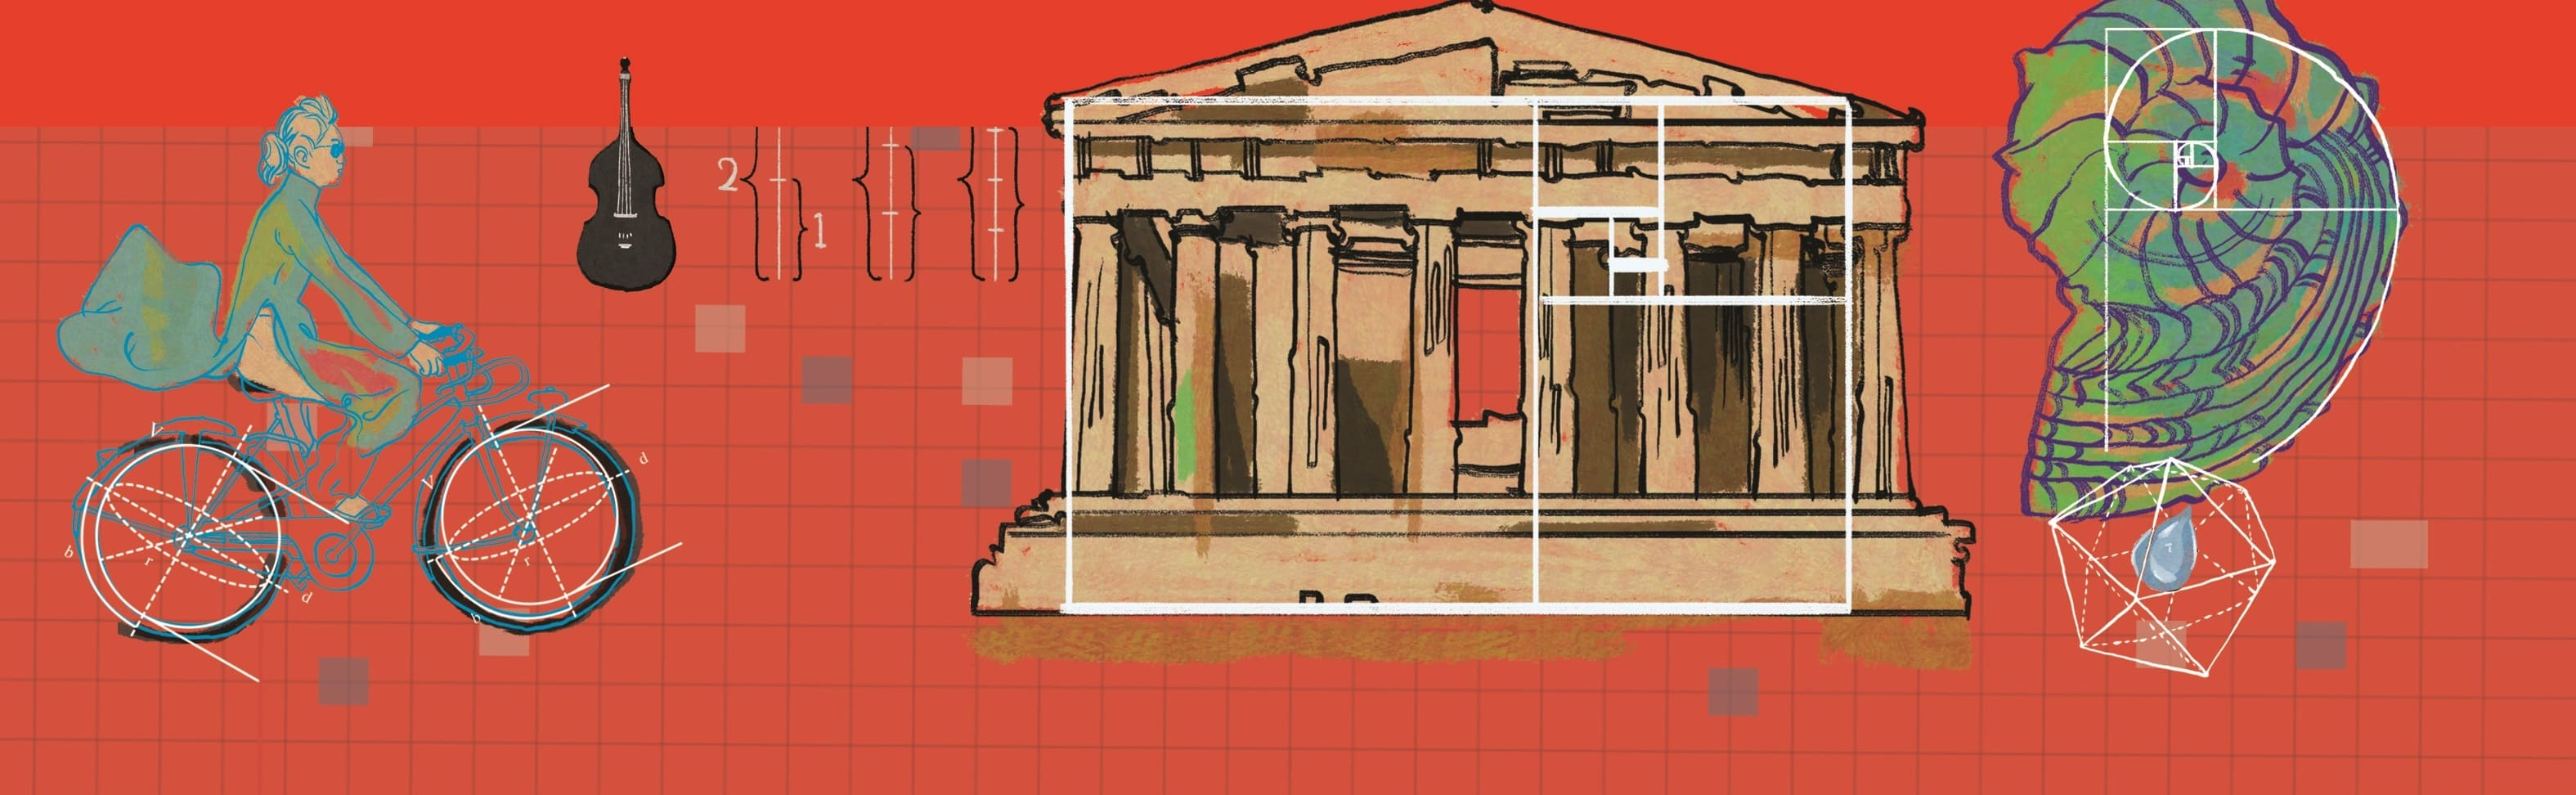
\includegraphics[width=19.3cm]{../bannertoanhocdoisong}}}
\AddToShipoutPicture*{\put(79,520){
\includegraphics[scale=1]{../tieude.pdf}}}
\centering
\endgroup

\vspace*{190pt}

\begin{multicols}{2}
	Bài toán cây kim của Buffon vẫn luôn xuất hiện trong sách giáo khoa toán dưới dạng một phương pháp để tính số $\pi$. Trong bài này, chúng ta hãy cũng Pi tìm hiểu chi tiết về bài toán này cũng như một số ứng dụng thú vị của nó trong thực tiễn.
	
	\vskip 0.1cm
	\textbf{\color{toanhocdoisong}$\pmb{1.}$ Bài toán cây kim của Buffon}
	\begin{figure}[H]
		\vspace*{-5pt}
		\centering
		\captionsetup{labelformat= empty, justification=centering}
		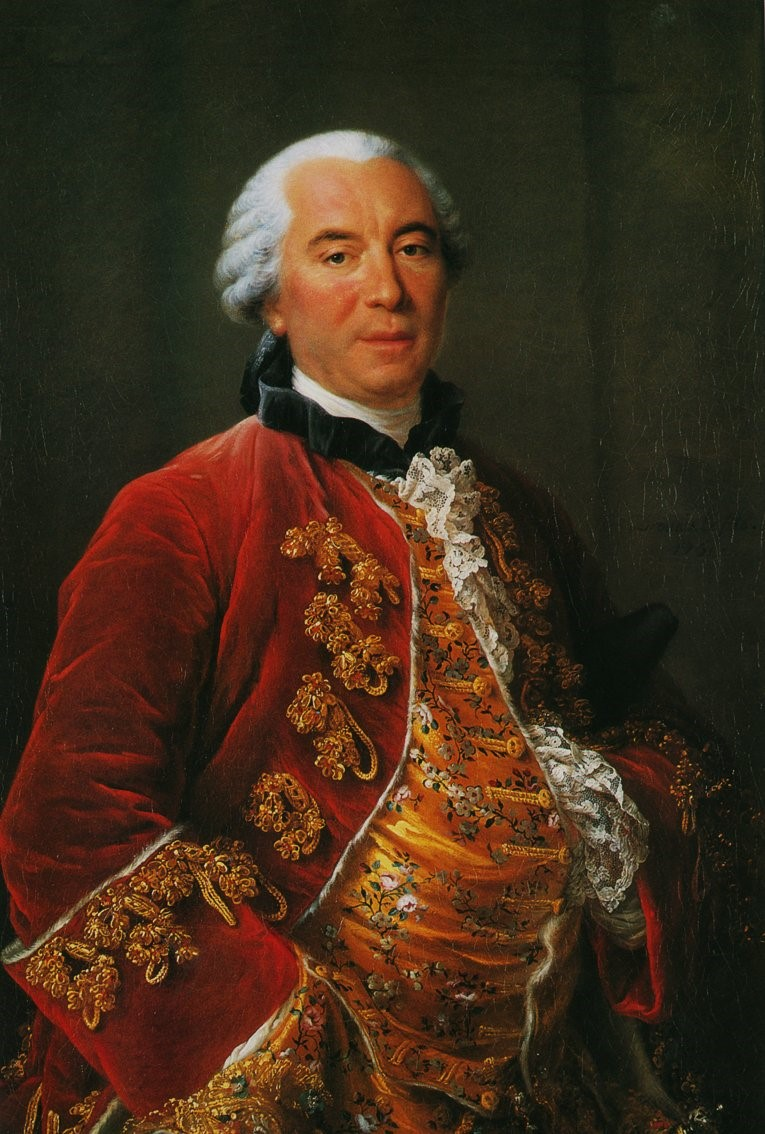
\includegraphics[width=0.6\linewidth]{1}
		\caption{\small\textit{\color{toanhocdoisong}Georges--Louis Leclerc, Comte de Buffon $(1707-1788)$.}}
		\vspace*{-10pt}
	\end{figure}
	Nhà toán học Pháp thế kỉ $18$, Georges Louis Leclerc, được phong Bá tước tại vùng có một ngôi làng tên Buffon nên ông còn có danh hiệu Comte de Buffon (Bá tước Buffon). Do đó các tài liệu thường gọi tắt là Buffon. Bài toán nổi tiếng mang tên ông có nội dung như sau:
	\vskip 0.1cm
	``Trên một tờ giấy với các đường kẻ cách đều nhau khoảng cách $d$, thả ngẫu nhiên một cây kim chiều dài $l$ $(d>l)$, hãy tìm xác suất để cây kim cắt một đường nằm ngang trên trang giấy".
	\begin{figure}[H]
		\vspace*{-5pt}
		\centering
		\captionsetup{labelformat= empty, justification=centering}
		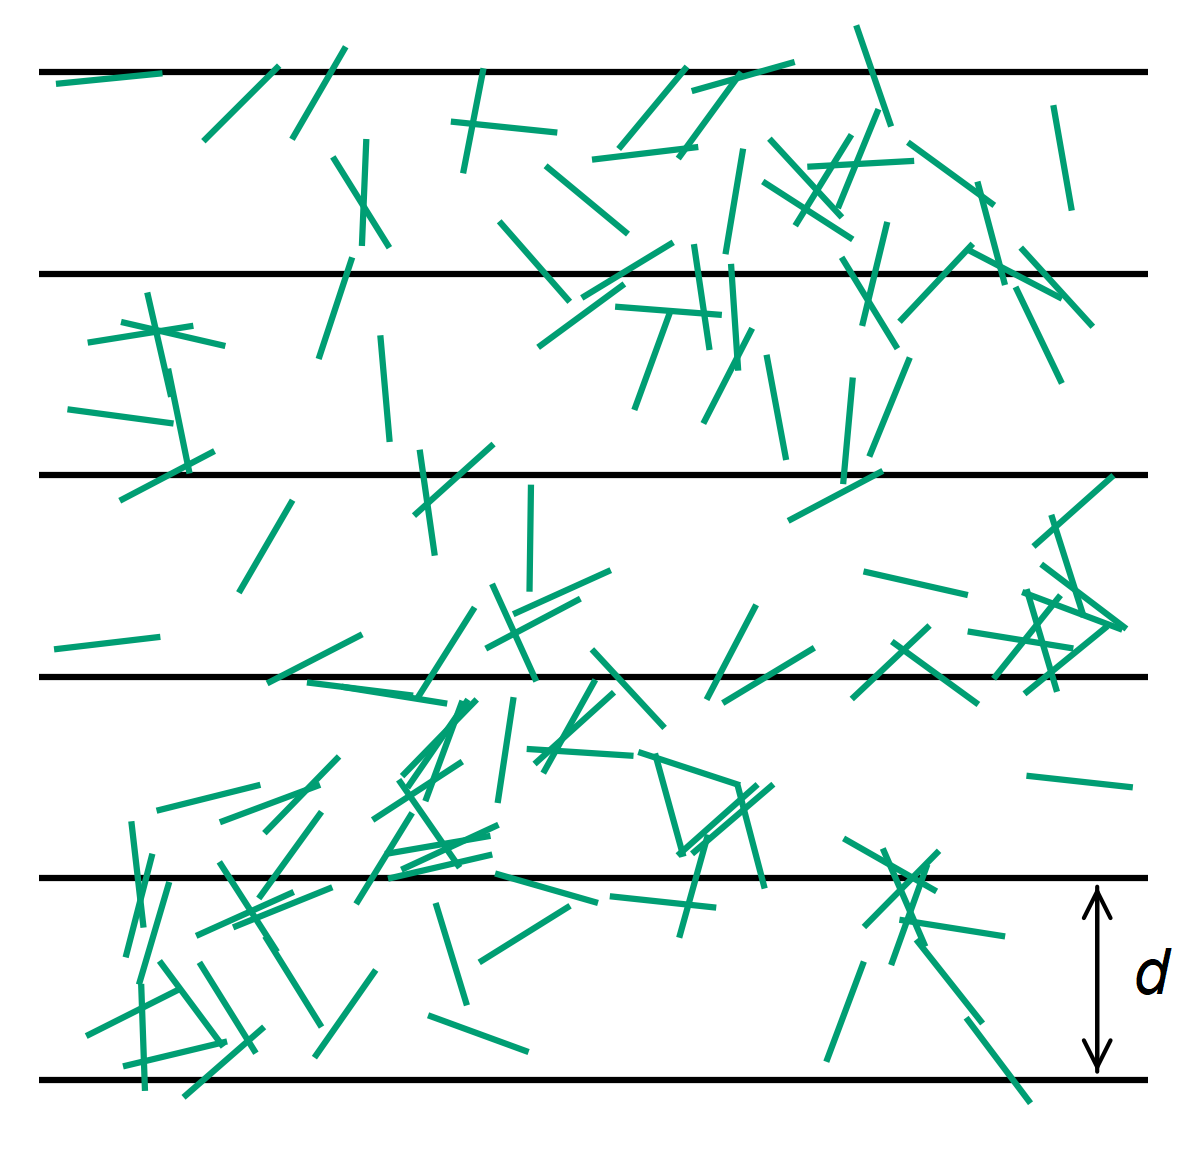
\includegraphics[width=0.95\linewidth]{2}
		\caption{\small\textit{\color{toanhocdoisong}Hình $1$. Minh họa bài toán cây kim của Buffon.}}
		\vspace*{-10pt}
	\end{figure}
	Chúng ta hãy xét một lời giải không sử dụng tích phân được E. Barbier đưa ra năm $1860$.
	\vskip 0.1cm 
	Do $l<d$ nên chỉ có hai trường hợp xảy ra: cây kim cắt một đường kẻ và cây kim không đè lên đường kẻ nào; không tồn tại trường hợp cây kim cắt nhiều hơn một đường kẻ.
	\vskip 0.1cm
	Gọi $P(l)$ là xác suất để cây kim có độ dài $l$ cắt một đường kẻ khi được thả. Lấy một điểm bất kỳ trên cây kim chia nó thành hai đoạn thẳng độ dài $l_1$ và $l_2$. Ta có:
	\begin{align*}
		P(l)=P(l_1 )+P(l_2).
	\end{align*}
	Quan hệ trên có thể được mở rộng ra thành dạng $P(l)=n\cdot P(\dfrac{l}{n})$. Tức là xác suất để một cây kim cắt đường kẻ khi được thả sẽ bằng $n$ lần xác suất này của cây kim có độ dài bằng $\dfrac{1}{n}$ lần độ dài cây kim ban đầu.
	\vskip 0.1cm
	Do đó, $P(l)=c\cdot l$ với $c$ là một hằng số, $c=P(1)$ (khi $l=1$ và $d > 1$).
	\begin{figure}[H]
		\vspace*{-5pt}
		\centering
		\captionsetup{labelformat= empty, justification=centering}
		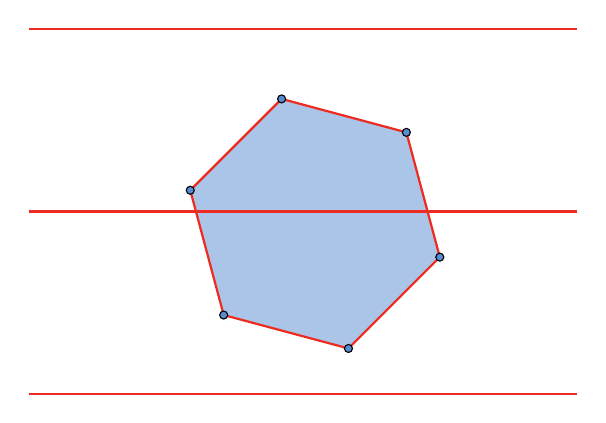
\begin{tikzpicture}[scale=0.58]
			\definecolor{qqqqff}{rgb}{0.,0.,1.}
			\definecolor{ududff}{rgb}{0.30196078431372547,0.30196078431372547,1.}
				\fill[line width=0.8pt,color=cackithi,fill=cackithi,fill opacity=0.5] (1.,3.) -- (3.,5.) -- (2.267949192431123,7.732050807568878) -- (-0.46410161513775494,8.464101615137755) -- (-2.4641016151377553,6.464101615137756) -- (-1.7320508075688794,3.7320508075688785) -- cycle;
				\draw [line width=0.8pt,color=toanhocdoisong] (1.,3.)-- (3.,5.);
				\draw [line width=0.8pt,color=toanhocdoisong] (3.,5.)-- (2.267949192431123,7.732050807568878);
				\draw [line width=0.8pt,color=toanhocdoisong] (2.267949192431123,7.732050807568878)-- (-0.46410161513775494,8.464101615137755);
				\draw [line width=0.8pt,color=toanhocdoisong] (-0.46410161513775494,8.464101615137755)-- (-2.4641016151377553,6.464101615137756);
				\draw [line width=0.8pt,color=toanhocdoisong] (-2.4641016151377553,6.464101615137756)-- (-1.7320508075688794,3.7320508075688785);
				\draw [line width=0.8pt,color=toanhocdoisong] (-1.7320508075688794,3.7320508075688785)-- (1.,3.);
				\draw [toanhocdoisong,line width=0.8pt] (-6.,6.)-- (6.,6.);
				\draw [toanhocdoisong,line width=0.8pt] (-6.,2.)-- (6.,2.);
				\draw [toanhocdoisong,line width=0.8pt] (-6.,10.)-- (6.,10.);
			
				\draw [fill=cackithi] (1.,3.) circle (2.5pt);
				\draw [fill=cackithi] (3.,5.) circle (2.5pt);
				\draw [fill=cackithi] (2.267949192431123,7.732050807568878) circle (2.5pt);
				\draw [fill=cackithi] (-0.46410161513775494,8.464101615137755) circle (2.5pt);
				\draw [fill=cackithi] (-2.4641016151377553,6.464101615137756) circle (2.5pt);
				\draw [fill=cackithi] (-1.7320508075688794,3.7320508075688785) circle (2.5pt);
		\end{tikzpicture}
		\caption{\small\textit{\color{toanhocdoisong}Hình $2$. Thả một đa giác cạnh $l$ lên tờ giấy với các đường kẻ ngang cách đều nhau.}}
		\vspace*{-10pt}
	\end{figure}
	Ta hãy tiếp tục xét một đa giác đều $N$ cạnh có độ dài mỗi cạnh bằng $l$ (Hình $2$). Ta đã biết ở trên rằng xác suất để mỗi cạnh của đa giác cắt một đường kẻ là $P(l)$. Đây cũng chính là giá trị kỳ vọng của số giao điểm của một cạnh với các đường kẻ, vì số giao điểm nói chung chỉ có thể là $0$ hoặc $1$ tương ứng với không cắt và cắt. Theo tính chất cộng tính của kỳ vọng, giá trị kỳ vọng của số giao điểm của đa giác với các đường kẻ khi thả lên tờ giấy là:
	\begin{align*}
		E &= \sum\nolimits_{i = 1}^N {P(l) = N \cdot } P(l) \\
		&= N \cdot c \cdot l = c \cdot L, \tag{$1$}
	\end{align*}
	với $L=N \cdot l$ là chu vi của đa giác đều.
	\vskip 0.1cm
	\columnbreak
	\PIbox{\textbf{\color{toanhocdoisong}Giá trị kỳ vọng}
		\vskip 0.1cm
		Trong một thí nghiệm ngẫu nhiên, nếu kết quả có giá trị $x_i$ có xác suất xảy ra là $p_i$ thì giá trị kỳ vọng của kết quả thu được được tính theo công thức:
		\setlength{\abovedisplayskip}{4pt}
		\setlength{\belowdisplayskip}{4pt}
		\begin{align*}
			E=x_1 p_1+x_2 p_2+ \cdots +x_n p_n.
		\end{align*}
		Ví dụ, với thí nghiệm gieo con xúc xắc, giá trị kỳ vọng của số chấm thu được là:
		\begin{align*}
			E=\frac{1}{6}\cdot 1 + \frac{1}{6} \cdot 2 + \cdots + \frac{1}{6}\cdot6 = 3{,5}.
		\end{align*}
		Chú ý rằng giá trị kỳ vọng có thể không trùng với một trong các giá trị có thể xảy ra. Theo định luật số lớn trong xác suất, với số lần thực hiện thí nghiệm càng lớn thì giá trị trung bình của các kết quả sẽ càng đến gần với giá trị kỳ vọng.}
	\vskip 0.1cm
	Mặt khác, nếu giữ chu vi $L$ của đa giác không đổi, khi $N \to \infty$, đa giác của ta sẽ trở thành một đường tròn có chu vi $L$ và bán kính $\dfrac{L}{2\pi}$.
	\vskip 0.1cm
	Để tính hệ số $c$, ta xét một trường hợp đặc biệt, khi đường tròn có đường kính đúng bằng khoảng cách $d$ giữa các dòng kẻ. Khi đó, ta có $L=\pi d$.
	\begin{figure}[H]
		\vspace*{-5pt}
		\centering
		\captionsetup{labelformat= empty, justification=centering}
		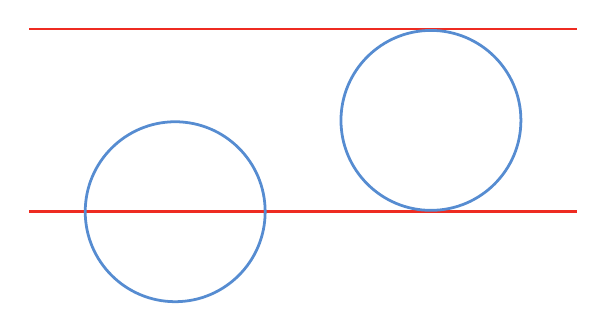
\begin{tikzpicture}[scale=0.58]
			\draw [toanhocdoisong, line width=1.pt] (-6.,6.)-- (6.,6.);
			\draw [toanhocdoisong, line width=1.pt] (-6.,10.)-- (6.,10.);
			\draw [cackithi, line width=1.pt] (2.8,8.) circle (1.97cm);
			\draw [cackithi, line width=1.pt] (-2.8,6.) circle (1.97cm);
		\end{tikzpicture}
		\caption{\small\textit{\color{toanhocdoisong}Hình $3$. Đường tròn có đường kính $d$ sẽ luôn cắt một đường kẻ tại hai điểm hoặc tiếp xúc hai đường kẻ.}}
		\vspace*{-10pt}
	\end{figure}
	Đường tròn có đường kính $d$ sẽ luôn cắt một đường kẻ tại $2$ giao điểm hoặc tiếp xúc với $2$ đường kẻ liên tiếp, do đó với đường tròn này $E=2$. Thay vào ($1$) ta có:
	\begin{align*}
		2=c\cdot\pi d
	\end{align*}
	hay $c = \dfrac{2}{\pi d}$.
	\vskip 0.1cm
	Vậy xác suất để một cây kim khi thả cắt đường nằm ngang trên giấy là 
	\begin{align*}
		P(l) = \frac{2l}{\pi d}. \tag{$2$}
	\end{align*}
	\begin{figure}[H]
		\vspace*{-5pt}
		\centering
		\captionsetup{labelformat= empty, justification=centering}
		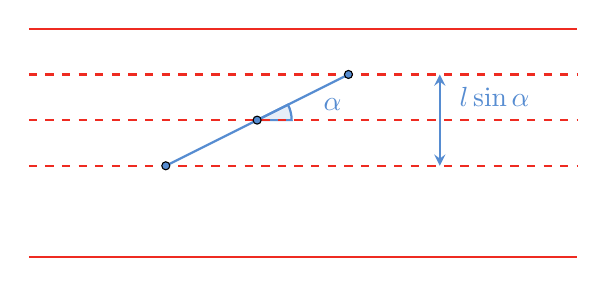
\begin{tikzpicture}[scale=0.58]
			\draw [shift={(-1.,8.)},line width=0.8pt,color=cackithi,fill=cackithi,fill opacity=0.15000000596046448] (0,0) -- (0.:0.7555063451882832) arc (0.:26.56505117707799:0.7555063451882832) -- cycle;
			\draw [toanhocdoisong,line width=0.8pt] (-6.,10.)-- (6.,10.);
			\draw [toanhocdoisong,dashed, line width=0.8pt] (-6.,9.)-- (6.,9.);
			\draw [toanhocdoisong,dashed, line width=0.8pt] (-6.,8.)-- (6.,8.);
			\draw [toanhocdoisong,dashed, line width=0.8pt] (-6.,7.)-- (6.,7.);
			\draw [toanhocdoisong, line width=0.8pt] (-6.,5.)-- (6.,5.);
			\draw [cackithi,line width=0.8pt] (-3.,7.)-- (1.,9.);
			\draw [fill=cackithi] (-3,7) circle (2.5pt);
			\draw [fill=cackithi] (1,9) circle (2.5pt);
			\draw [fill=cackithi] (-1,8) circle (2.5pt);
			\draw [cackithi,-stealth,line width=0.8pt] (3.,8.)-- (3.,9.);
			\draw [cackithi,-stealth,line width=0.8pt] (3.,8.)-- (3.,7.);
			
			\draw[color=cackithi] (0.65,8.347966297286694) node {$\color{cackithi}\alpha$};
			\draw[color=cackithi] (4.2,8.5) node {$\color{cackithi}l\sin\alpha$};
		\end{tikzpicture}
		\caption{\small\textit{\color{toanhocdoisong}Hình $4$. Chứng minh công thức $(2)$ sử dụng tích phân.}}
		\vspace*{-10pt}
	\end{figure}
	Ta cũng có thể thu được đáp án này bằng cách sử dụng tích phân. Cụ thể là ta xây dựng một mô hình xác suất cho vị trí rơi của cây kim. Gọi $\alpha$ $(0\le \alpha \le \dfrac{\pi}{2})$ là góc mà cây kim tạo với phương nằm ngang. Hình chiếu của nó theo phương vuông góc với các đường kẻ sẽ có độ dài $l\sin\alpha$, mà khoảng cách giữa hai đường kẻ là $d$, do đó xác suất để nó cắt một đường kẻ là $\dfrac{l\sin\alpha}{d}$. Coi phân bố của $\alpha$ là đều trên khoảng $[0,\dfrac{\pi}{2}]$, ta tính giá trị trung bình bằng cách lấy tích phân trên khoảng này rồi chia cho $\dfrac{\pi}{2}$ để thu được ($2$):
	\begin{align*}
		P(l) &= \frac{2}{\pi }\int_0^{\frac{\pi }{2}} {\frac{{l\sin \alpha }}{d}} d\alpha  = \frac{2}{\pi }\frac{l}{d}\left[ { - \cos \alpha } \right]|_0^{\frac{\pi }{2}}\\
		& = \frac{2}{\pi }\frac{l}{d}.
	\end{align*}
	Với cây kim có độ dài lớn hơn $d$, xác suất để nó cắt ít nhất một đường kẻ trong khoảng $\left[\arcsin\left(\dfrac{d}{l}, \dfrac{\pi}{2}\right)\right]$ sẽ luôn là $1$, do đó:
	\begin{align*}
		&P(l) \\
		= \,&\frac{2}{\pi }\left( {\int_0^{\arcsin \left( {\frac{d}{l}} \right)} {\frac{{l\sin \alpha }}{d} + } \int_{\arcsin \left( {\frac{d}{l}} \right)}^{\frac{\pi }{2}} {1d\alpha } } \right)\\
		=\,&1 \!\!+\!\! \frac{2}{\pi }\!\left( \!\!{\frac{l}{d}\!\!\left(\!\! {1 \!-\! \sqrt {\!\!1 \!-\! \frac{{{d^2}}}{{{l^2}}}} \!} \right) \!\!-\! \arcsin\! \frac{d}{l}}\! \right)\!\!.\tag{$3$}
	\end{align*}
	Bài toán này cũng được Laplace mở rộng cho trường hợp lưới trên tờ giấy là lưới chữ nhật và  tính xác suất để cây kim không cắt một đường kẻ dọc hay ngang nào. 
	\vskip 0.1cm
	Cũng chính Laplace đã đề xuất sử dụng thí nghiệm này để tính giá trị của số $\pi$. Đây cũng là khía cạnh được biết đến nhiều nhất về bài toán cây kim của Buffon. Thật vậy, nếu trong $M$ lần thả cây kim, ta thu được $m$ lần mà nó cắt một đường kẻ, công thức ($2$) cho ta:
	\begin{align*}
		\pi = \frac{2l}{d\cdot\left(\frac{m}{M}\right)},
	\end{align*}
	với $\dfrac{m}{M}$ là xác suất thực nghiệm của sự kiện cây kim cắt một đường kẻ.
	\vskip 0.1cm
	Đề xuất này của Laplace rất gần với phương pháp Monte Carlo của hơn một thế kỉ sau. Tuy vậy, về mặt thực tế, nó gập phải một số vấn đề. Nhiều thí nghiệm được tiến hành và cho kết quả của $\pi$ không quá chính xác: $3{,}1596$; $3{,}1553$; $3{,}137$.
	\vskip 0.1cm 
	Năm $1901$, Lazzarini công bố giá trị $3{,}1415929$ cho $3408$ lần thả cây kim, một giá trị khá chính xác (so với giá trị đã biết hiện nay, thì chỉ có chữ số cuối là không đúng). Tuy vậy, một số nghiên cứu đã chỉ ra kết quả này hầu như là ngụy tạo. Theo các lí thuyết về ước lượng tham số, để có độ chính xác đến $6$ chữ số sau dấu phẩy, cần phải tiến hành thí nghiệm trên $1{,}34×10^{14}$ lần chứ không phải vài nghìn lần. Đồng thời, số liệu của Lazzarini sử dụng phân số $\dfrac{355}{113}$, một số hữu tỉ được biết là một xấp xỉ tốt cho $\pi$. 
	\vskip 0.1cm
	Ngay cả với máy tính điện tử thì việc ước lượng $\pi$ bằng cách sử dụng thí nghiệm Buffon cũng không đạt được độ chính xác quá cao do việc làm tròn số trên máy tính. Đồng thời, các chữ số của $\pi$ cũng có thể được tính toán một cách chính xác hơn bởi các phương pháp khác.
	\vskip 0.1cm
	Tuy vậy, bài toán cây kim của Buffon có một ý nghĩa quan trọng trong lịch sử toán học bởi sự liên hệ giữa xác suất và hình học. Đây là một hướng tiếp cận mới khác với hướng tiếp cận xác suất sử dụng tổ hợp như truyền thống.
	\vskip 0.1cm
	\textbf{\color{toanhocdoisong}Bài tập}
	\vskip 0.1cm
	$1$. Chứng minh rằng khi cây kim vô cùng dài thì một cách hầu chắc chắn nó sẽ luôn cắt ít nhất một đường kẻ, tức là biểu thức trong ($3$) có giới hạn là $1$ khi $l\to \infty$.
	\vskip 0.1cm
	$2$. Trên tờ giấy với các đường kẻ ngang cách nhau khoảng $d$, thả ngẫu nhiên một đường tròn với bán kính $r < \dfrac{d}{2}$. Hãy tính xác suất để đường tròn cắt và không cắt các đường kẻ.
	\vskip 0.1cm
	$3$. Tương tự bài trên nhưng thả một hình vuông có cạnh $a<d$. Hãy tính xác suất để số giao điểm của các cạnh hình vuông với các đường kẻ ngang là:
	\vskip 0.1cm
	$a)$ $0$\quad\quad		$b)$ $1$\quad\quad		$c)$ $2$\quad\quad
	$d)$ $3$\quad\quad		$e)$ $4$
	\vskip 0.1cm
	Gợi ý: Xét trường hợp $a<\dfrac{d}{\sqrt{2}}$ và $a> \dfrac{d}{\sqrt{2}}$.
	\vskip 0.1cm	
	$4$. Trong thí nghiệm Buffon, với cây kim có độ dài $l>d$, hãy chứng minh giá trị kỳ vọng của số giao điểm của cây kim với các đường kẻ ngang là $E = \dfrac{2l}{\pi d}$. (Gợi ý: Gọi $N$ là số nguyên lớn nhất sao cho $d<\dfrac{l}{N}$, coi cây kim là hình gồm $N$ đoạn thẳng bằng nhau).
	\vskip 0.1cm
	$5$. Mở rộng của Laplace. Trên một lưới chữ nhật, với mỗi hình chữ nhật có chiều dài $a$ và chiều rộng $b$, thả ngẫu nhiên một cây kim chiều dài $l$ (biết rằng $l$ nhỏ hơn cả $a$ và $b$). Hãy tính xác suất để cây kim không chạm bất kỳ cạnh nào của lưới.
	\vskip 0.1cm
	$6$. Lưới Uspensky. Cho một lưới tam giác đều như hình vẽ với $d$ là chiều cao của mỗi tam giác đều. Thả một cây kim chiều dài \linebreak$l<d$ lên lưới tam giác đều này. Hãy tính xác suất để số giao điểm của cây kim với các đường trong lưới là:
	\vskip 0.1cm
	\quad\quad$a)$ $0$\quad\quad		$b)$ $1$\quad\quad		$c)$ $2$	\quad\quad	$d)$ $3$
	\begin{figure}[H]
		\vspace*{5pt}
		\centering
		\captionsetup{labelformat= empty, justification=centering}
		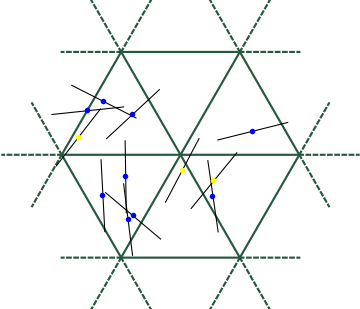
\includegraphics[width=1\linewidth]{6}
		\vspace*{-15pt}
	\end{figure}
	$7$. Bài toán sợi mì của Buffon. Trên một tờ giấy với các đường kẻ ngang song song cách nhau khoảng $d$, ném ngẫu nhiên một sợi mì ướt có độ dài $l$. Chứng minh rằng giá trị kì vọng của số giao điểm của sợi mì với các đường kẻ ngang là $E=\dfrac{2l}{\pi d}$. Giả sử rằng khi ném sợi mì, chiều dài của nó không đổi nhưng nó có thể uốn thành một đường cong bất kỳ.
	\vskip 0.1cm
	\textbf{\color{toanhocdoisong}$\pmb{2.}$ Đo độ dài bằng phương pháp ngẫu nhiên}
	\vskip 0.1cm
	Với một số thay đổi, thí nghiệm của Buffon có thể được sử dụng để giải quyết một vấn đề thực tế trong khoa học: đo độ dài của rễ cây (Newman, $1966$). Xét một bản thủy tinh mà trên đó một mẫu vật (ví dụ rễ cây) được trải phẳng. Khi quan sát mẫu vật qua kính hiển vi, người ta sử dụng một thị kính với một đường sợi tóc để soi các vùng khác nhau của bản thủy tinh.
	\vskip 0.1cm
	Với mỗi lần quan sát, thị kính được quay một góc bất kì và đường sợi tóc cũng được quay theo. Sau đó, số giao điểm của đường sợi tóc với rễ cây sẽ được ghi lại. Cách thức này được lặp lại nhiều lần với các vị trí quan sát ngẫu nhiên khác nhau trên bản thủy tinh. Để tiện lợi hơn, ta có thể đặt bản thủy tinh trên một tấm giấy với các điểm ngẫu nhiên đã được đánh dấu trước. Các điểm quan sát cũng có thể là một lưới ô vuông các điểm cách đều.
	\begin{figure}[H]
%		\vspace*{5pt}
		\centering
		\captionsetup{labelformat= empty, justification=centering}
		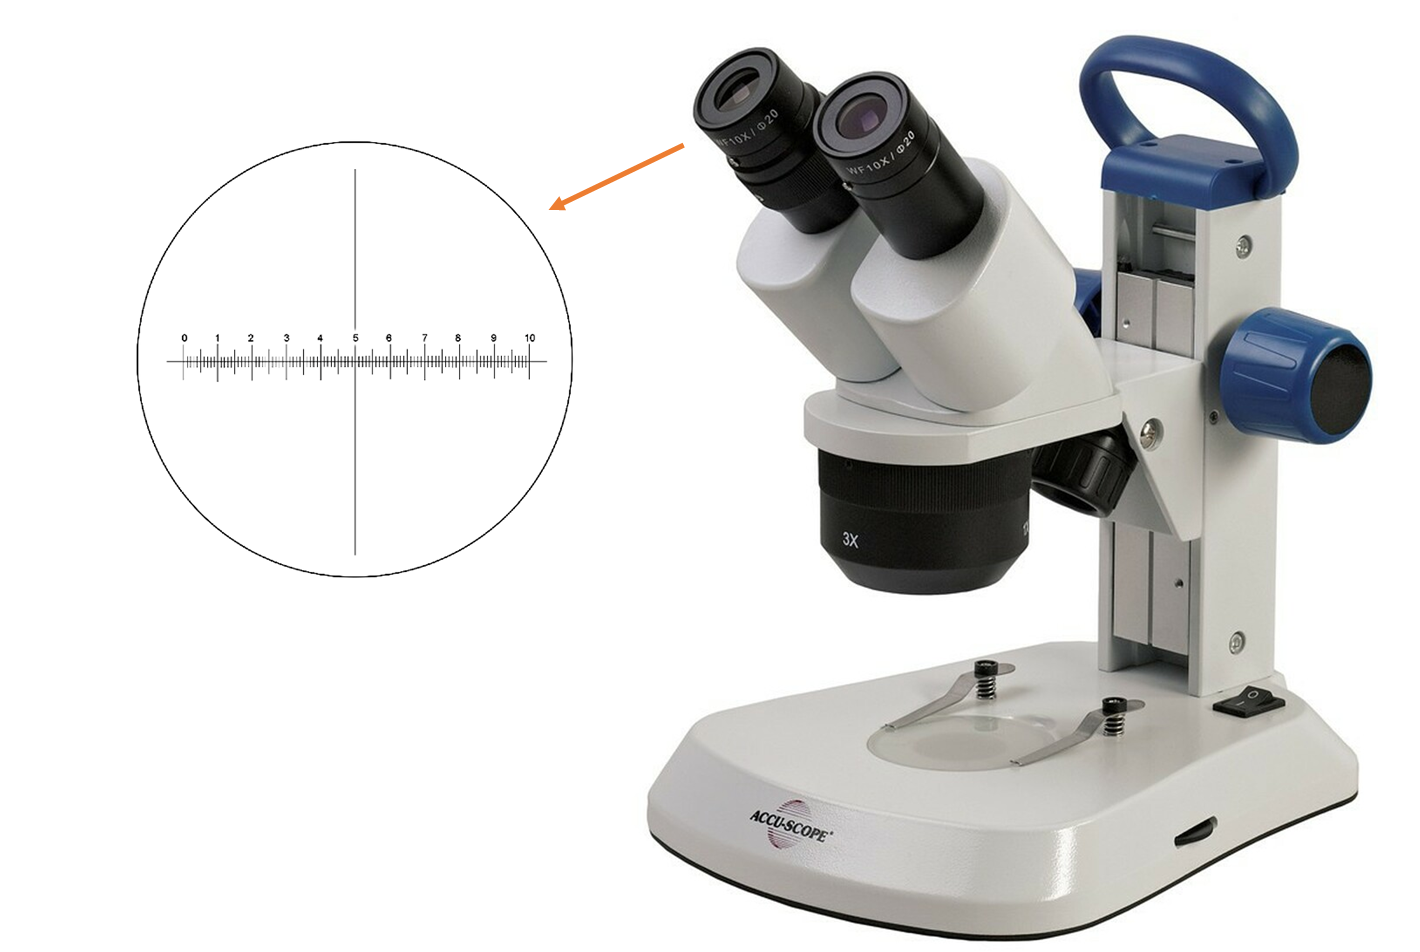
\includegraphics[width=1\linewidth]{7}
		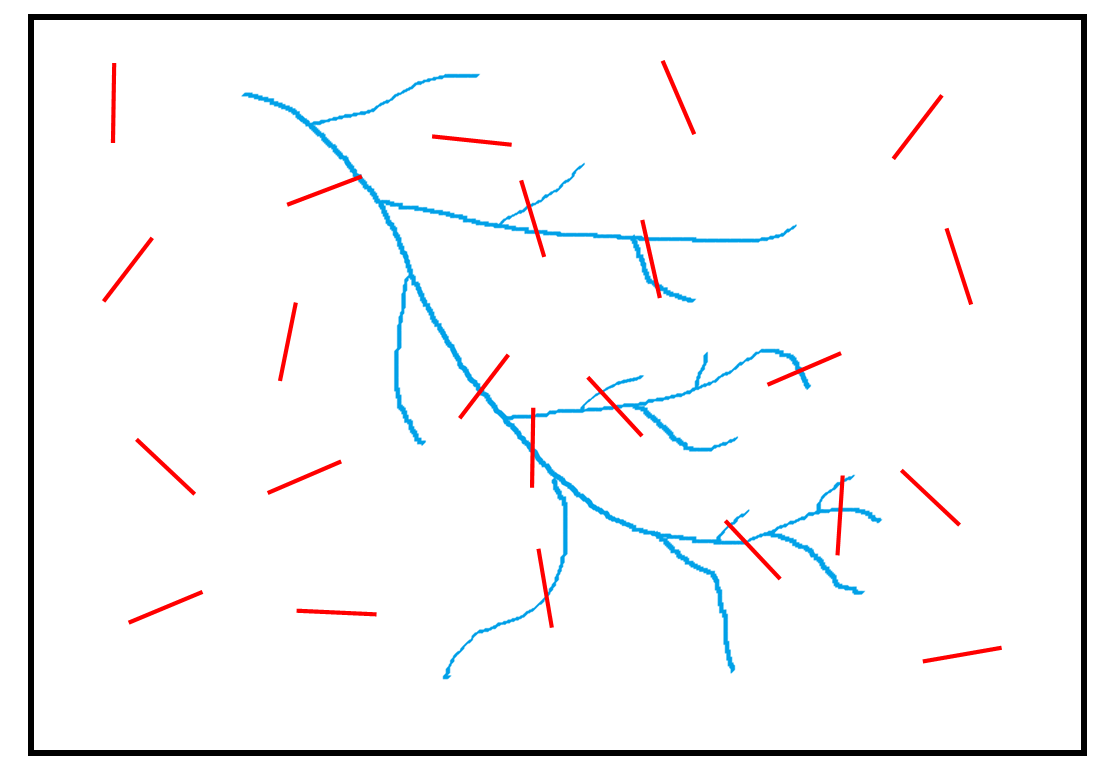
\includegraphics[width=1\linewidth]{8}
		\caption{\small\textit{\color{toanhocdoisong}Hình $5$. Trên: Thị kính của kính hiển vi có đường sợi tóc (đường thẳng đứng). Dưới: minh họa phép đo độ dài rễ cây (màu xanh) với các vị trí và góc quay khác nhau của đường sợi tóc (màu đỏ). Số lượng đường sợi tóc trong hình chỉ mang tính minh họa, trong thực tế, cấu trúc rễ cây càng phức tạp thì số lượng đường sợi tóc cần sử dụng lại càng nhiều. Mỗi lần quan sát qua kính, ta chỉ thấy được một vùng hình tròn có đường kính là đường sợi tóc.}}
		\vspace*{-10pt}
	\end{figure}
	Về mặt bản chất, thay vì đếm số giao điểm của cây kim được thả ngẫu nhiên với các đường kẻ ngang, ta đếm số giao điểm của các đường sợi tóc được phân bố ngẫu nhiên với mẫu vật rễ cây (gồm nhiều đường cong) trên bản thủy tinh.
	\vskip 0.1cm
	Độ dài của rễ cây có thể được tính theo công thức:
	\begin{align*}
		R= \frac{\pi N A}{2H},	\tag{$4$}
	\end{align*}
	với $N$ là số giao điểm đã được đếm, $A$ là diện tích bản thủy tinh và $H$ là tổng độ dài của tất cả các đường sợi tóc.
	\vskip 0.1cm
	Thật vậy, xét một đoạn rễ cây $PQ$ có chiều dài $\Delta R$ và một đường sợi tóc $MN$ chiều dài $h$. Nếu khoảng cách từ trung điểm $D$ của $PQ$ đến $MN$ lớn hơn $\dfrac{1}{2}\Delta R$ thì $PQ$ và $MN$ chắc chắn không cắt nhau. Miền giới hạn này được biểu diễn bằng đường nét đứt trong hình. Giả sử $\dfrac{\Delta R}{h}$ là nhỏ, diện tích miền này có thể được xấp xỉ bằng $\Delta R \cdot h$. Do $MN$ được phân bố ngẫu nhiên trên bản thủy tinh, xác suất để $D$ nằm trong miền này là $\dfrac{\Delta R \cdot h}{A}$.
	\vskip 0.1cm
	Khi $D$ nằm trong miền cách $MN$ một khoảng không quá $\dfrac{1}{2}\Delta R$, khoảng cách từ $D$ đến $MN$ cần phải không lớn hơn $\dfrac{1}{2}\Delta R |\sin \theta |$, với $\theta$ là góc tạo bởi hai đường thẳng $PQ$ và $MN$, để $PQ$ và $MN$ cắt nhau. Xác suất để $PQ$ và $MN$ cắt nhau khi $D$ đã nằm trong miền trên là:
	\begin{align*}
		\frac{\frac{1}{2}\Delta R|\sin\theta|}{\frac{1}{2}\Delta R} = |\sin\theta|.
	\end{align*}
	Do đó, theo công thức nhân xác suất, xác suất để $PQ$ và $MN$ cắt nhau là:
	\begin{align*}
		p = \frac{\Delta R\cdot h}{A} |\sin\theta|.
	\end{align*}
	\begin{figure}[H]
		\vspace*{-5pt}
		\centering
		\captionsetup{labelformat= empty, justification=centering}
		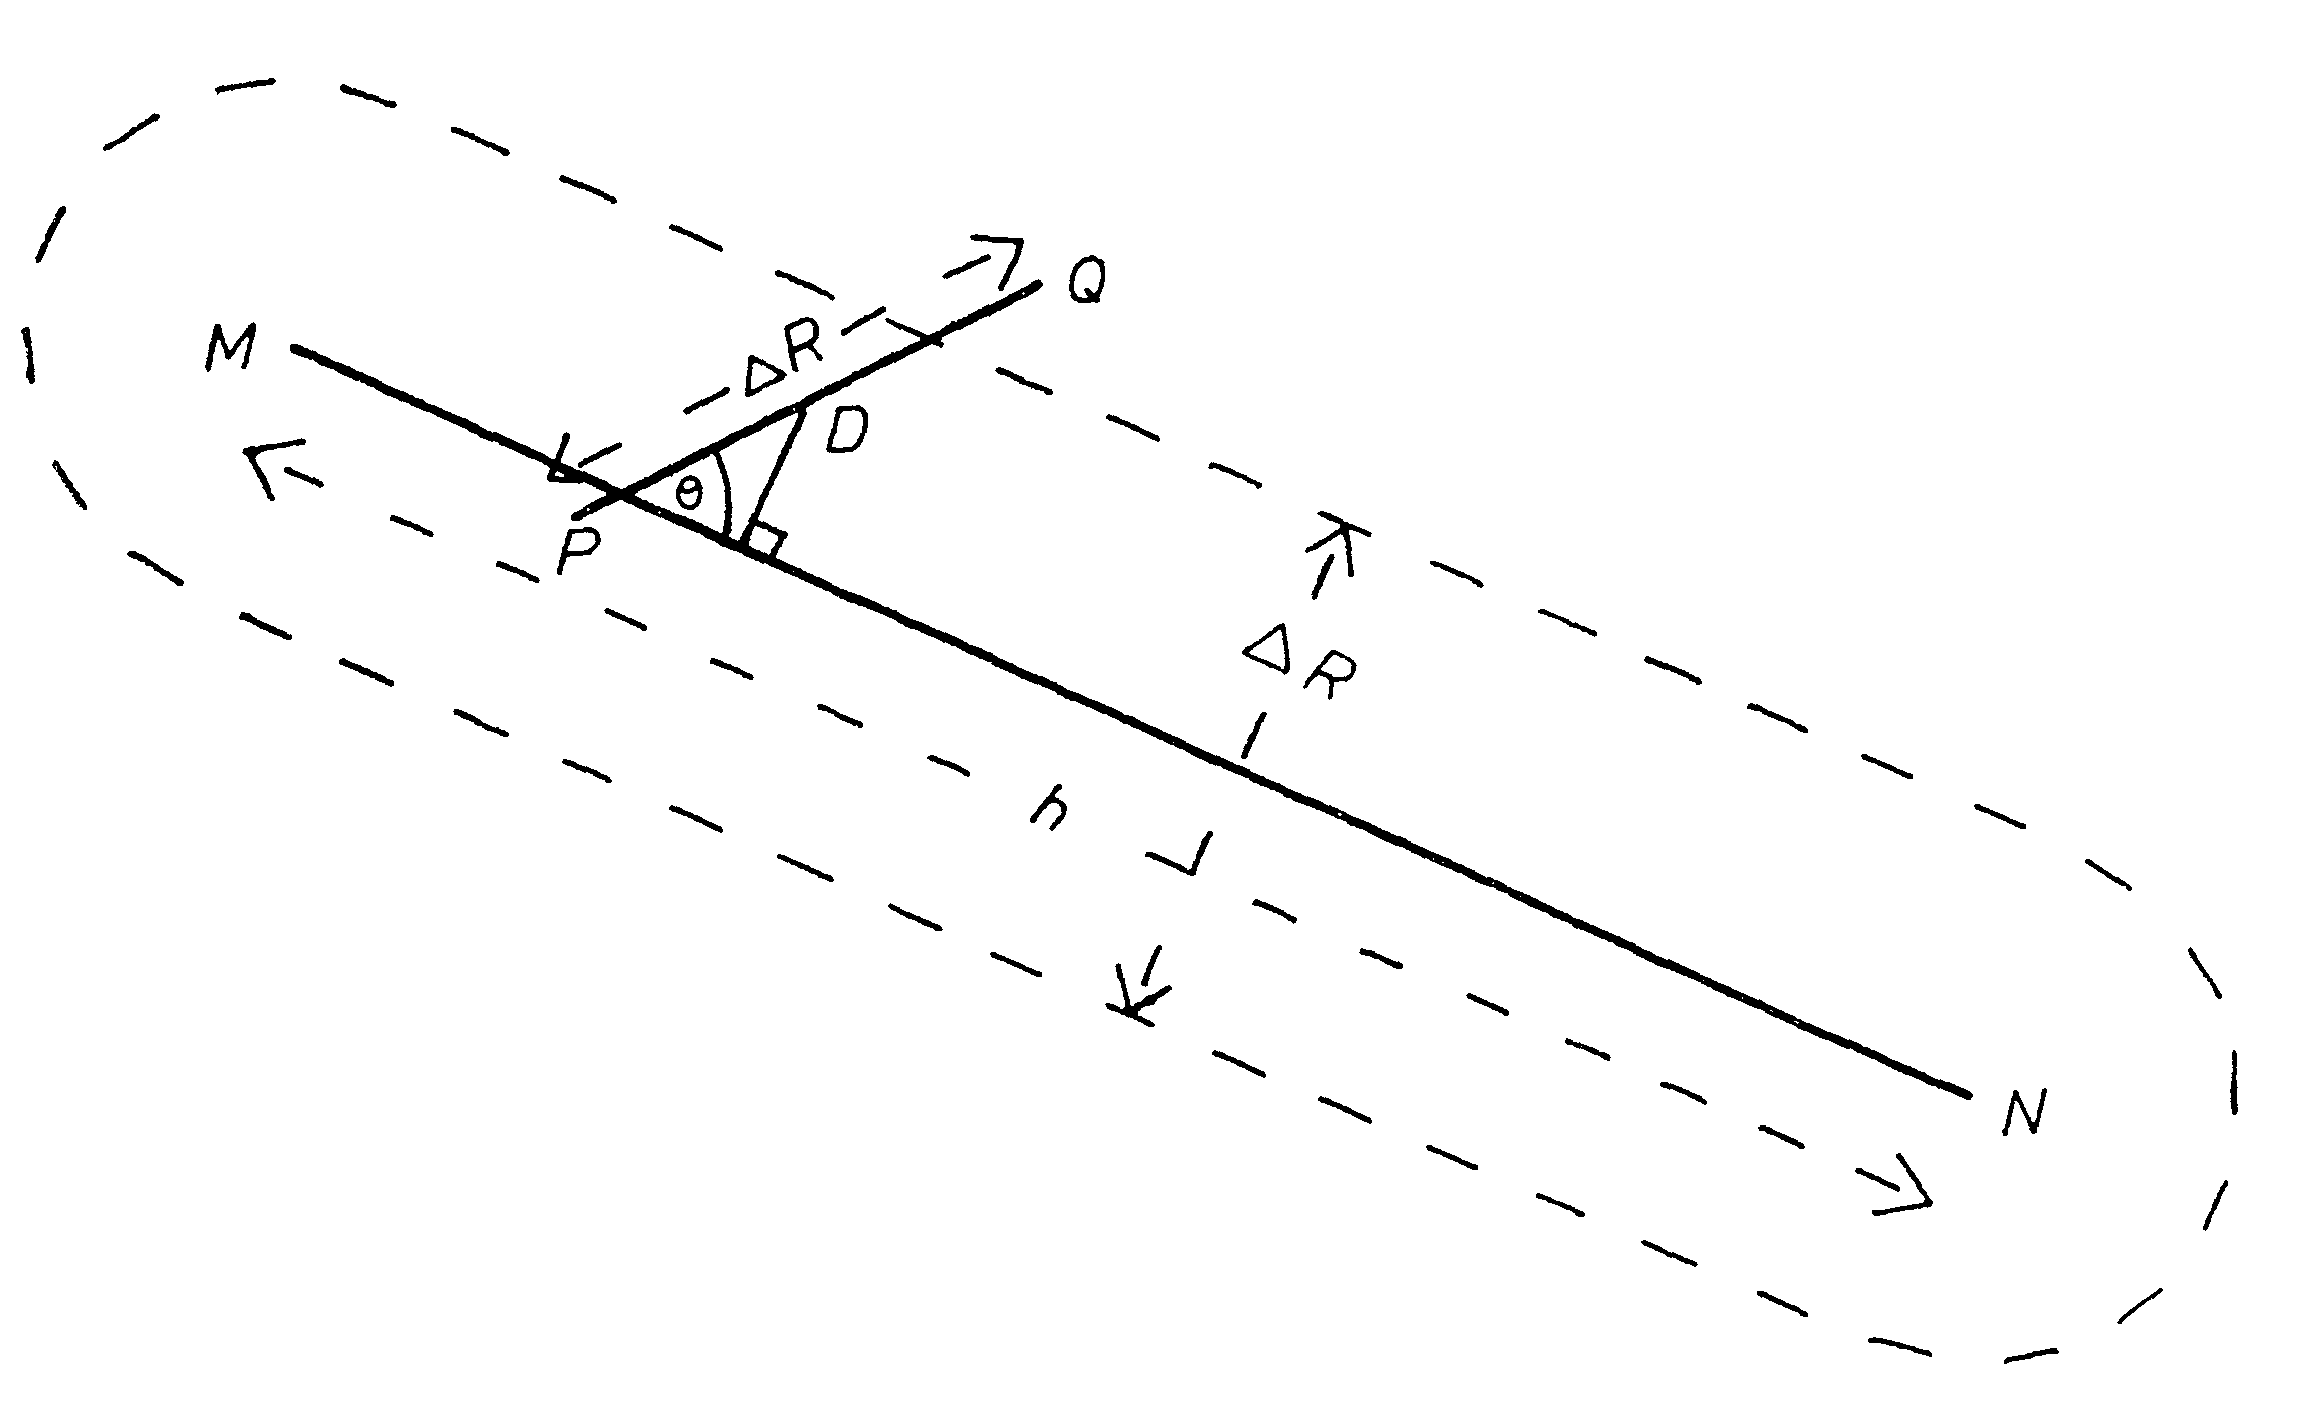
\includegraphics[width=1\linewidth]{9}
		\caption{\small\textit{\color{toanhocdoisong}Hình $6$. Đoạn rễ cây $PQ$ và đường sợi tóc $MN$.}}
		\vspace*{-10pt}
	\end{figure}
	Tổng độ dài của các đoạn sợi tóc được phân bố ngẫu nhiên trên miền diện tích $A$ là $H$. Các góc $\theta$ cũng nhận giá trị ngẫu nhiên trong khoảng $[0,2\pi]$ nên giá trị kì vọng của số giao điểm của $PQ$ với các đường sợi tóc là:
	\begin{align*}
		\frac{1}{2\pi}\int_0^{2\pi}{\frac{{\Delta R \cdot H}}{A}}|\sin\theta|d\theta= \frac{2\left(\Delta R \cdot H\right)}{\pi A}.
	\end{align*}
	Coi rễ cây là một hình với nhiều đoạn có độ dài $\Delta R$, ta được giá trị kì vọng của số giao điểm của rễ cây với tất cả các đường sợi tóc là:
	\begin{align*}
		N = \frac{2RH}{\pi A}.
	\end{align*}
	Do $N$ là giá trị kỳ vọng nên khi đo đạc người ta cần phải tiến hành nhiều lần quan sát với các vị trí ngẫu nhiên của đường sợi tóc để kết quả thí nghiệm gần với giá trị của $N$ trong công thức.
	\vskip 0.1cm
	Ví dụ, với bản thủy tinh $10\times 20$ cm; tiến hành quan sát $40$ lần, độ dài đường sợi tóc (đường kính của thị trường vùng quan sát được) là $1{,}88$ cm; số giao điểm quan sát được là $344$ thì tổng độ dài của rễ cây là:
	\begin{align*}
		R - \frac{\pi \cdot 344\cdot 10 \cdot 20}{2\cdot40 \cdot1{,}88} = 1436 \text{ cm}.
	\end{align*}
	Cách đo độ dài này đã được các nhà thực vật học sử dụng trong nhiều thập kỉ mãi cho đến gần đây mới được thay thế bởi các phần mềm xử lí ảnh từ các camera có độ phân giải cao.
	\vskip 0.1cm
	\textbf{\color{toanhocdoisong}$\pmb{3.}$ Kiến biết đo diện tích bằng xác suất?}
	\vskip 0.1cm
	Phương pháp đo độ dài ở phần trước cũng có thể được biến đổi để tiến hành đo diện tích.
	\vskip 0.1cm
	Một nghiên cứu khá thú vị trên loài kiến \textit{Leptothorax albipennis} đưa ra giả thuyết rằng loài kiến này đã sử dụng xác suất để tính diện tích khi chọn tổ (kiến thường cố gắng chọn tổ có diện tích lớn nhất trong các vị trí khảo sát) (Mallon \& Franks, $2000$).
	\vskip 0.1cm
	Khi sử dụng camera để theo dõi kiến trinh sát trong phòng thí nghiệm, người ta thấy trong lần thứ nhất đến một vị trí để khảo sát, con kiến sẽ đi một cách ngẫu nhiên trong hộp theo một đường cong bao phủ phần lớn các vị trí trong hộp (gọi là đường cong $L$). Trong những lần tiếp theo (thường nó sẽ quay lại lần thứ hai hoặc có thể là lần thứ $3$), nó sẽ đi một đường cong đơn giản hơn (gọi là đường cong $S$). Đồng thời, khi đến các vị trí đã đi qua (kiến khi di chuyển có thể tiết ra pheromone để đánh dấu đường đi của mình), tức là các giao điểm của $L$ và $S$, kiến dành thời gian lâu hơn nhiều.
	\begin{figure}[H]
		\vspace*{-5pt}
		\centering
		\captionsetup{labelformat= empty, justification=centering}
		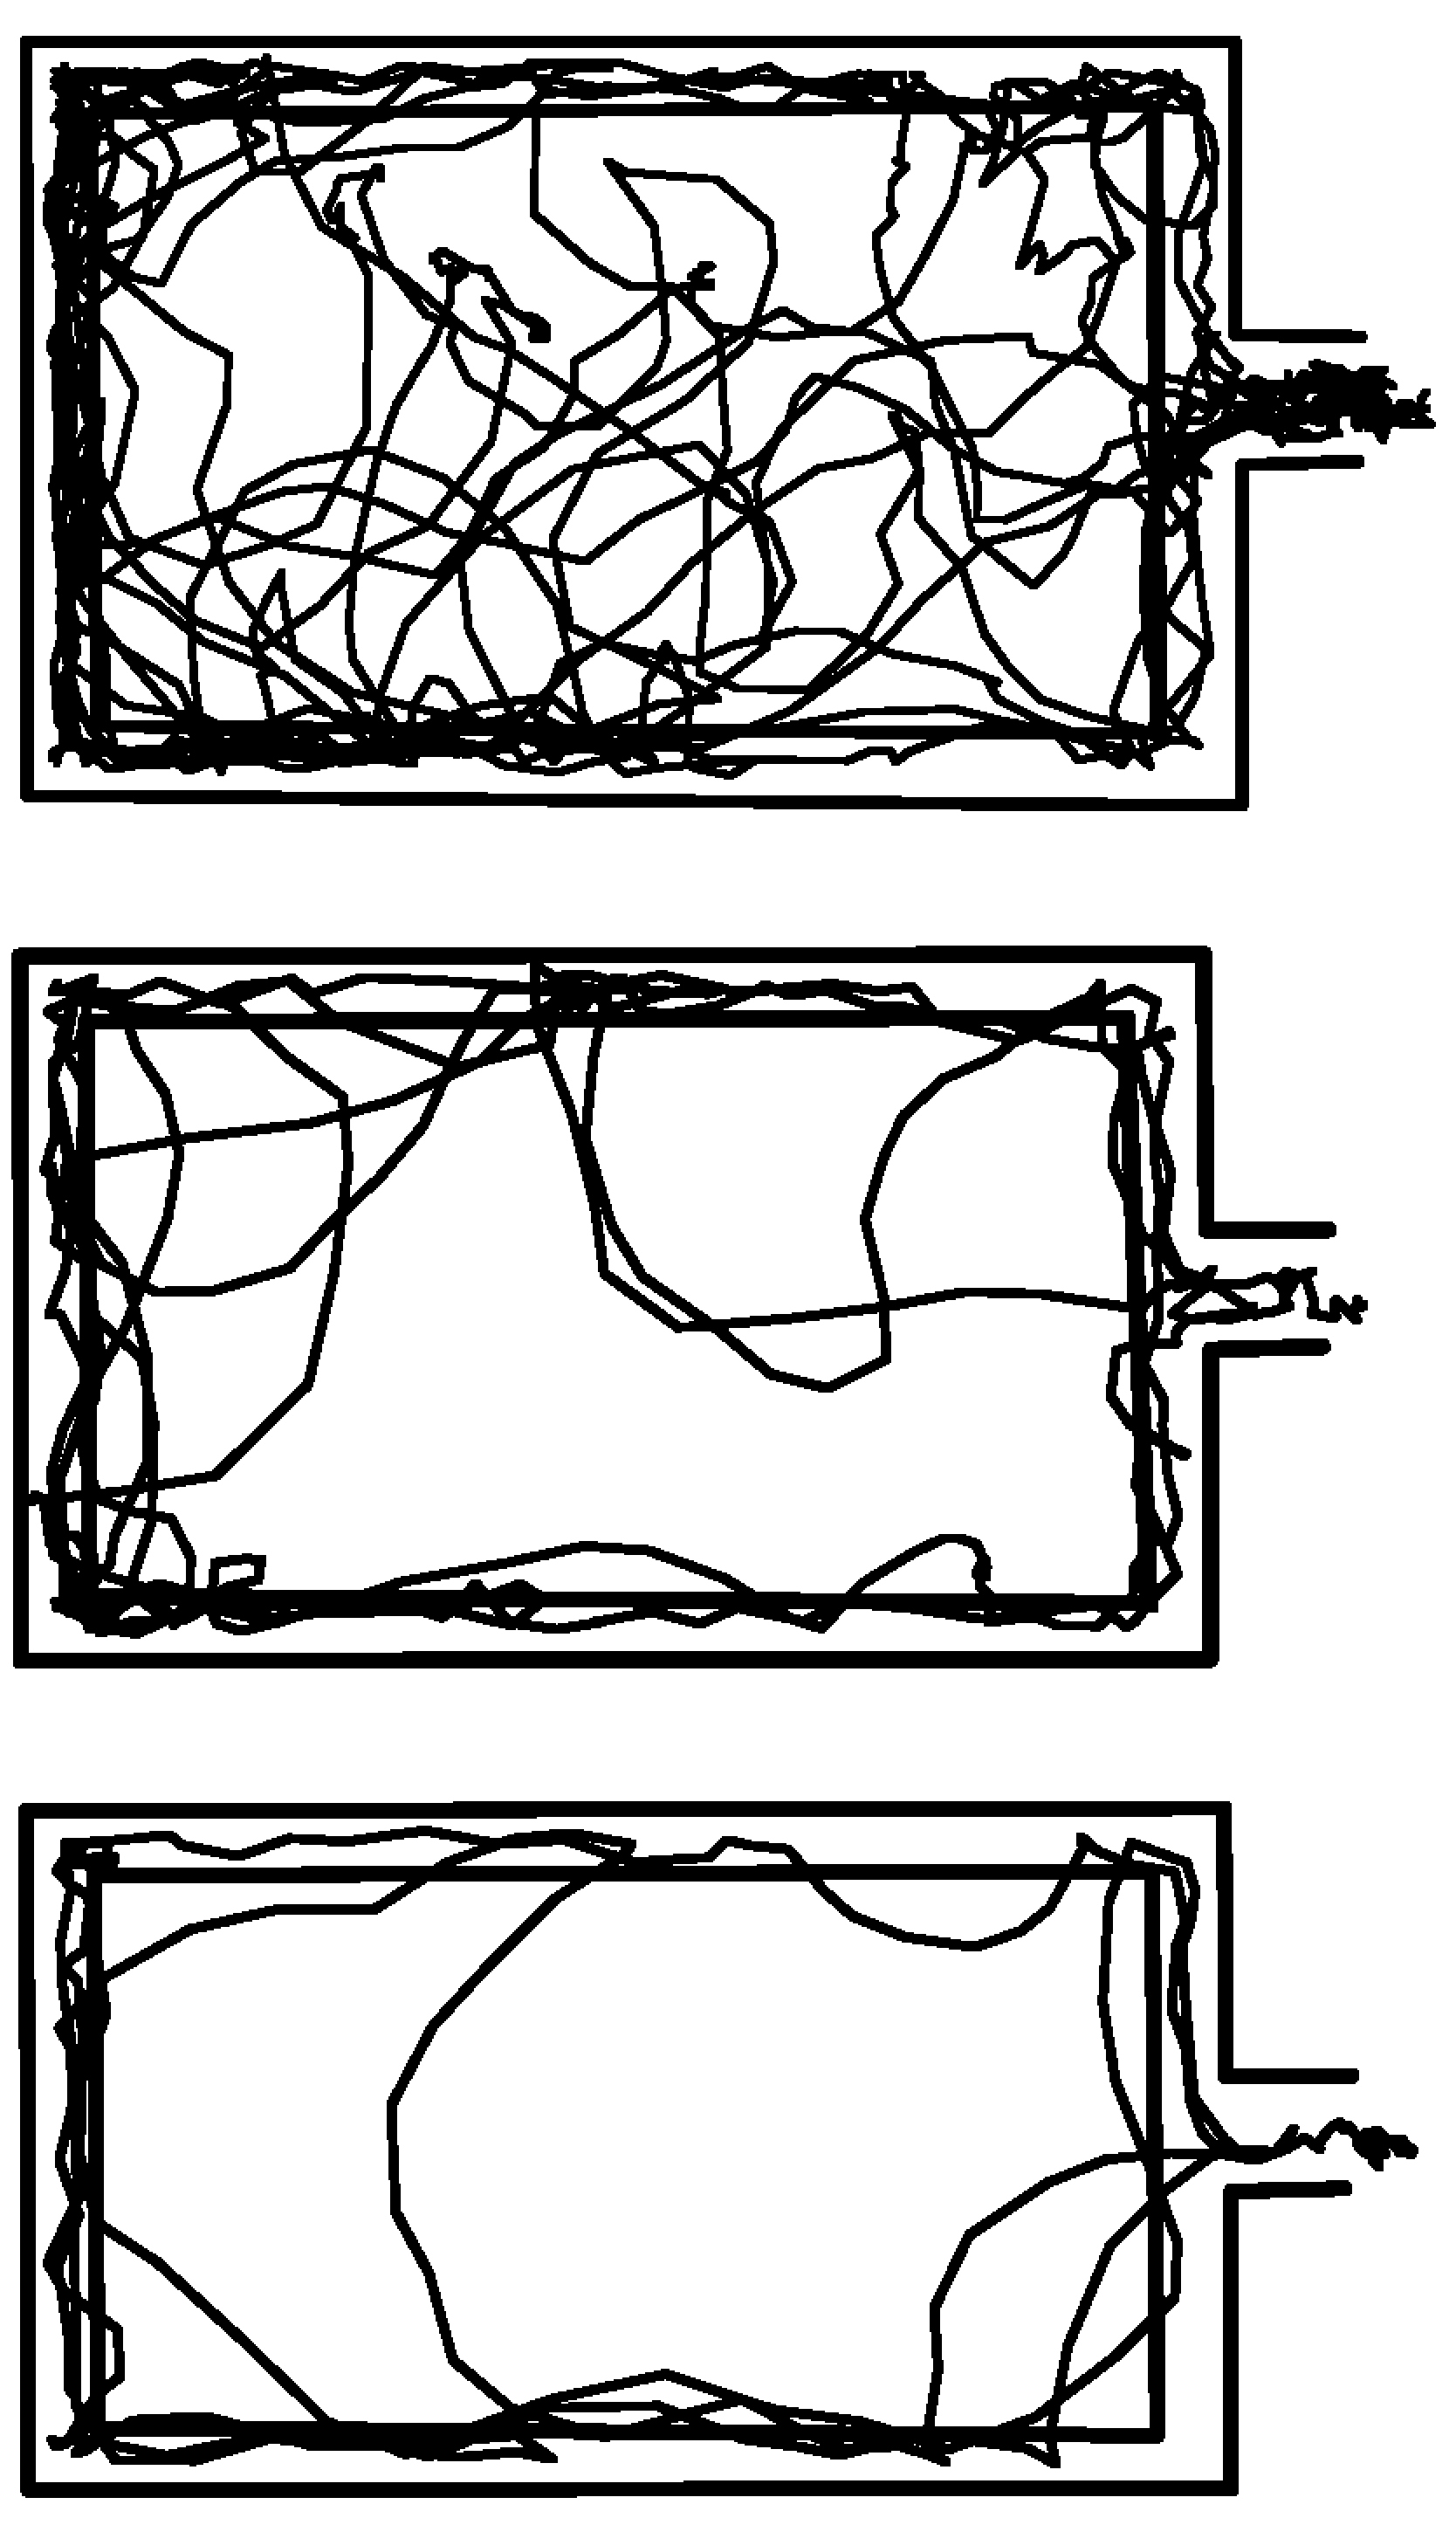
\includegraphics[width=0.65\linewidth]{10}
		\caption{\small\textit{\color{toanhocdoisong}Hình $7$. Từ trên xuống: Đường đi của kiến trinh sát khi khảo sát tổ được camera ghi lại trong lần khảo sát thứ nhất, thứ hai và thứ ba.}}
		\vspace*{-10pt}
	\end{figure}
	Theo các tác giả, số giao điểm của $L$ và $S$ được kiến trinh sát sử dụng để đánh giá diện tích của một vị trí làm tổ. Trong công thức ($4$), nếu ta thay các đường sợi tóc bằng một đường cong $L$ và rễ cây $R$ bằng đường cong $S$, công thức này vẫn đúng và diện tích có thể được xấp xỉ theo 
	\begin{align*}
		A = \frac{2SL}{\pi N}, \tag{$5$}
	\end{align*}
	với $N$ là số giao điểm của $S$ và $L$.
	\vskip 0.1cm
	Để kiểm chứng việc này, thí nghiệm được tiến hành với nhiều con kiến trinh sát khác nhau trên các loại hộp để làm tổ như trong hình vẽ.
	\vskip 0.1cm
	Trong thí nghiệm để chọn giữa hai tổ cùng chu vi (hình $8a$ và hình $8c$), kiến luôn chọn tổ có diện tích lớn hơn sau khi khảo sát cả hai. Do đó, diện tích chứ không phải chu vi mới là tiêu chí chọn tổ. Vì các tổ có một tấm chắn ở giữa (hình $8d$) cũng được chọn với khả năng tương tự như tổ bình thường, cho thấy số lần va chạm với chướng ngại vật trong tổ cũng không phải nhân tố quyết định.
	\begin{figure}[H]
		\vspace*{-5pt}
		\centering
		\captionsetup{labelformat= empty, justification=centering}
		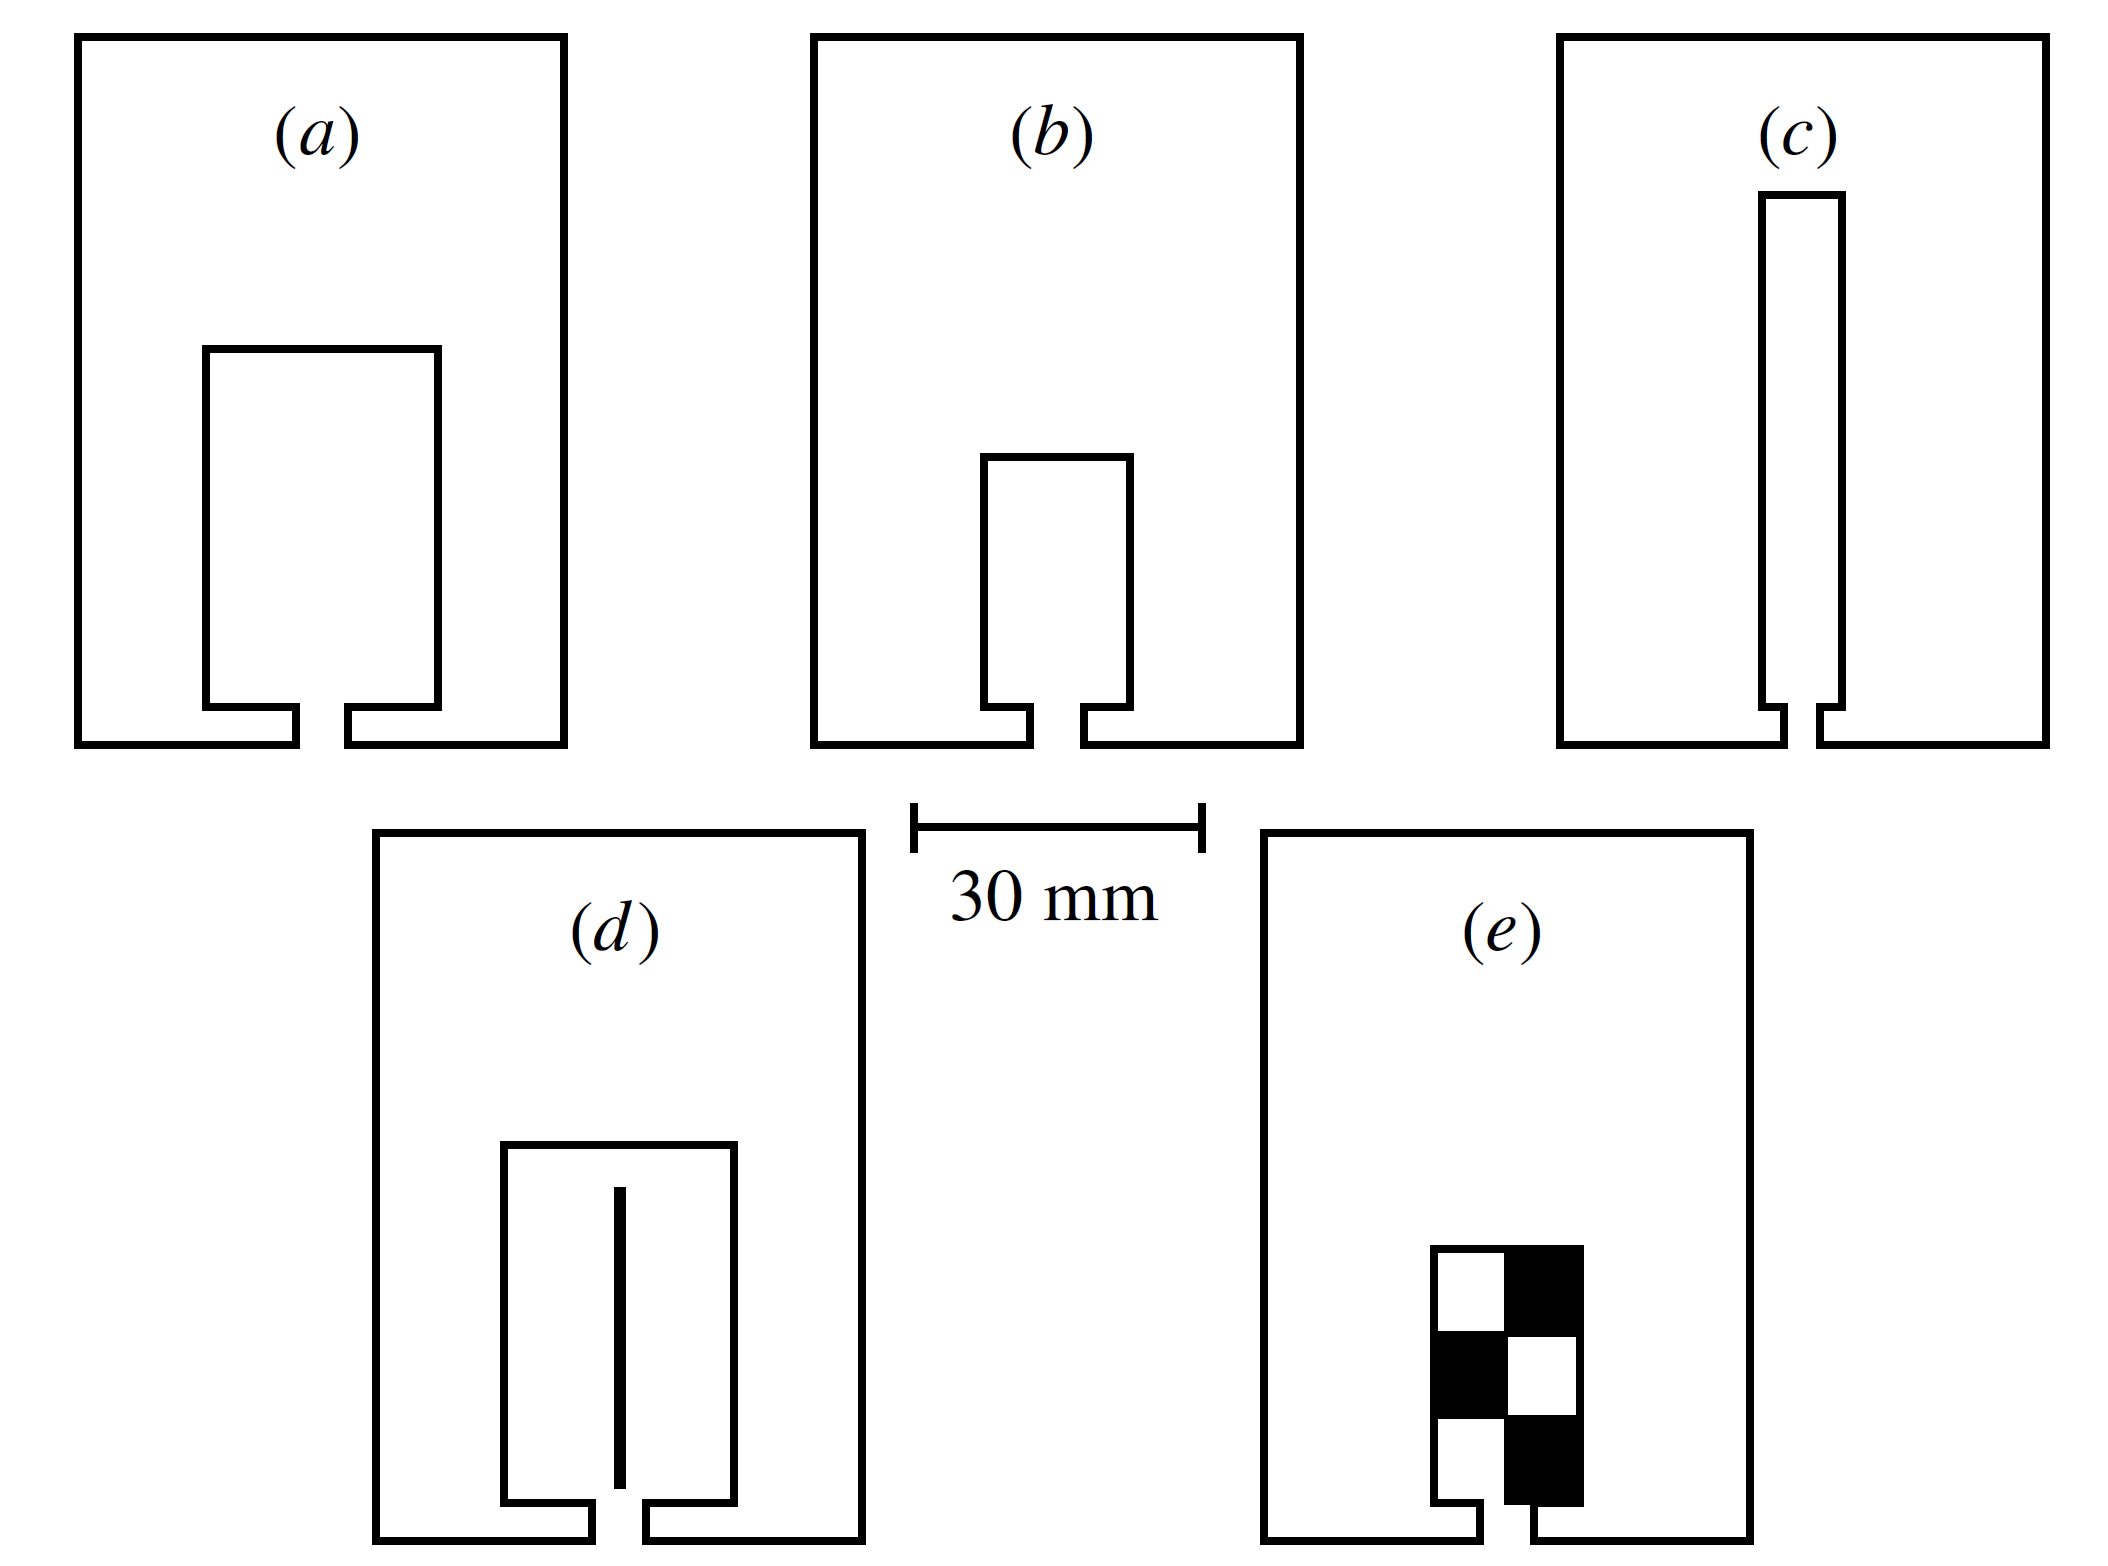
\includegraphics[width=1\linewidth]{11}
		\caption{\small\textit{\color{toanhocdoisong}Hình $8$. Các loại tổ được sử dụng trong thí nghiệm về việc chọn tổ của kiến trinh sát. $a)$ tổ tiêu chuẩn; $b)$ tổ đồng dạng và có diện tích bằng một nửa tổ tiêu chuẩn; $c)$ tổ có diện tích bằng một nửa tổ tiêu chuẩn nhưng có cùng chu vi; $d)$ tổ tiêu chuẩn có tấm chắn ở giữa; $e)$ tổ dạng $b$ với một nửa được phủ các tấm đệm có thể nhấc ra.}}
		\vspace*{-10pt}
	\end{figure}
	Thí nghiệm cũng cho thấy khi kiến trở lại lần thứ hai, nếu tổ đã được thay bằng một tổ mới hoặc một tổ đã được một con kiến khác đi qua, nó sẽ tiến hành khảo sát lại như là đang đi qua lần thứ nhất. Điều này cho thấy trong lần khảo sát thứ nhất, kiến sẽ lưu lại pheromone đánh dấu đường đi và pheromone này đặc trưng cho từng cá thể. Việc này cũng cho phép các con kiến không làm ảnh hưởng đến quá trình khảo sát của nhau khi một vị trí có thể được nhiều hơn một con kiến đến thăm dò.
	\vskip 0.1cm
	Nếu kiến trở lại lần thứ ba hoặc sau đó, thời gian nó tiến hành khảo sát cũng không khác nhiều lắm so với lần thứ hai, do đó có thể thấy pheromone chỉ được rải ở lần thăm dò thứ nhất còn các lần lặp lại sau để tăng độ chính xác của việc ước lượng.
	\vskip 0.1cm
	Loại tổ trong hình $8e$ được thiết kế đồng dạng với tổ trong hình $8a$ nhưng có diện tích bằng một nửa. Đồng thời, ở nền của loại tổ này, một nửa diện tích là các tấm đệm có thể lấy ra. Sau khi kiến khảo sát tổ dạng này lần thứ nhất, người ta sẽ lấy các tấm đệm ra trước khi kiến quay lại lần thứ hai. Khi kiến trở lại, do các vị trí có đệm bị lấy ra không còn pheromone nên số giao điểm của đường đi của nó trong lần thứ hai với đường đi trong lần thứ nhất sẽ giảm một nửa. Trong thí nghiệm chọn giữa tổ dạng $8a$ và dạng $8e$, một nửa số kiến chọn $8e$ dù diện tích chỉ có một nửa. Thí nghiệm với kích thước tổ lớn gấp đôi cho thấy khoảng cách $L$ của mỗi con kiến là không đổi giữa các tổ với diện tích khác nhau. Kết hợp với với ($5$), có thể thấy thấy kiến đánh giá diện tích theo tỉ lệ nghịch với tần số gặp giao điểm $\dfrac{N}{S}$.
	\vskip 0.1cm
	Việc nghiên cứu những thuật toán liên quan đến hành vi của kiến không chỉ có ý nghĩa về mặt sinh học mà còn có nhiều ứng dụng khác, ví dụ như trong việc lập trình điều khiển hành vi của robot.
	\vskip 0.1cm
	$\pmb{4.}$ \textbf{\color{toanhocdoisong}Lời kết}
	\vskip 0.1cm
	Lĩnh vực xác suất hình học còn có nhiều bài toán khác có giá trị về cả mặt lý thuyết lẫn thực tiễn. Pi cũng sẽ tiếp tục giới thiệu các bài toán này đến với độc giả trong tương lai không xa.
	\vskip 0.1cm
	\textbf{\color{toanhocdoisong}Tài liệu tham khảo}
	\vskip 0.1cm
	[$1$] Aigner, M., \& Ziegler, G. ($2004$). \textit{Proof from} THE BOOK. Springer--Verlag.
	\vskip 0.1cm
	[$2$] Mallon, E. B., \& Franks, N. R. ($2000$). Ants estimate area using Buffon's needle. \textit{Proc. R. Soc. Lond.} B($267$), $765-770$.
	\vskip 0.1cm
	[$3$] Mugford, S. T., Mallon, E. B., \& Franks, N. R. ($2001$). The accuracy of Buffon's needle: a rule of thumb used by ants to estimate area. \textit{Behavioral Ecology}, $12(6)$, $655-658$.
	\vskip 0.1cm
	[$4$] Newman, E. I. ($1966$). A Method of Estimating the Total Length of Root in a Sample. \textit{Journal of Applied Ecology}, $139-145$.
	\vskip 0.1cm
	[$5$] Ramaley, J. F. ($1969$). Buffon's Noodle Problem. \textit{The American Mathematical Monthly}, $78(8)$, $916-918$.
\end{multicols}
%	\newpage
%
%	\setcounter{figure}{0}
%	\thispagestyle{quantoannone}
\pagestyle{quantoan}
\everymath{\color{quantoan}}
\graphicspath{{../quantoan/pic/}}
\blfootnote{\color{quantoan}\color{quantoan}$^*$Nguồn Math. Intellegencer, Số $41$.}
\begingroup
\AddToShipoutPicture*{\put(0,616){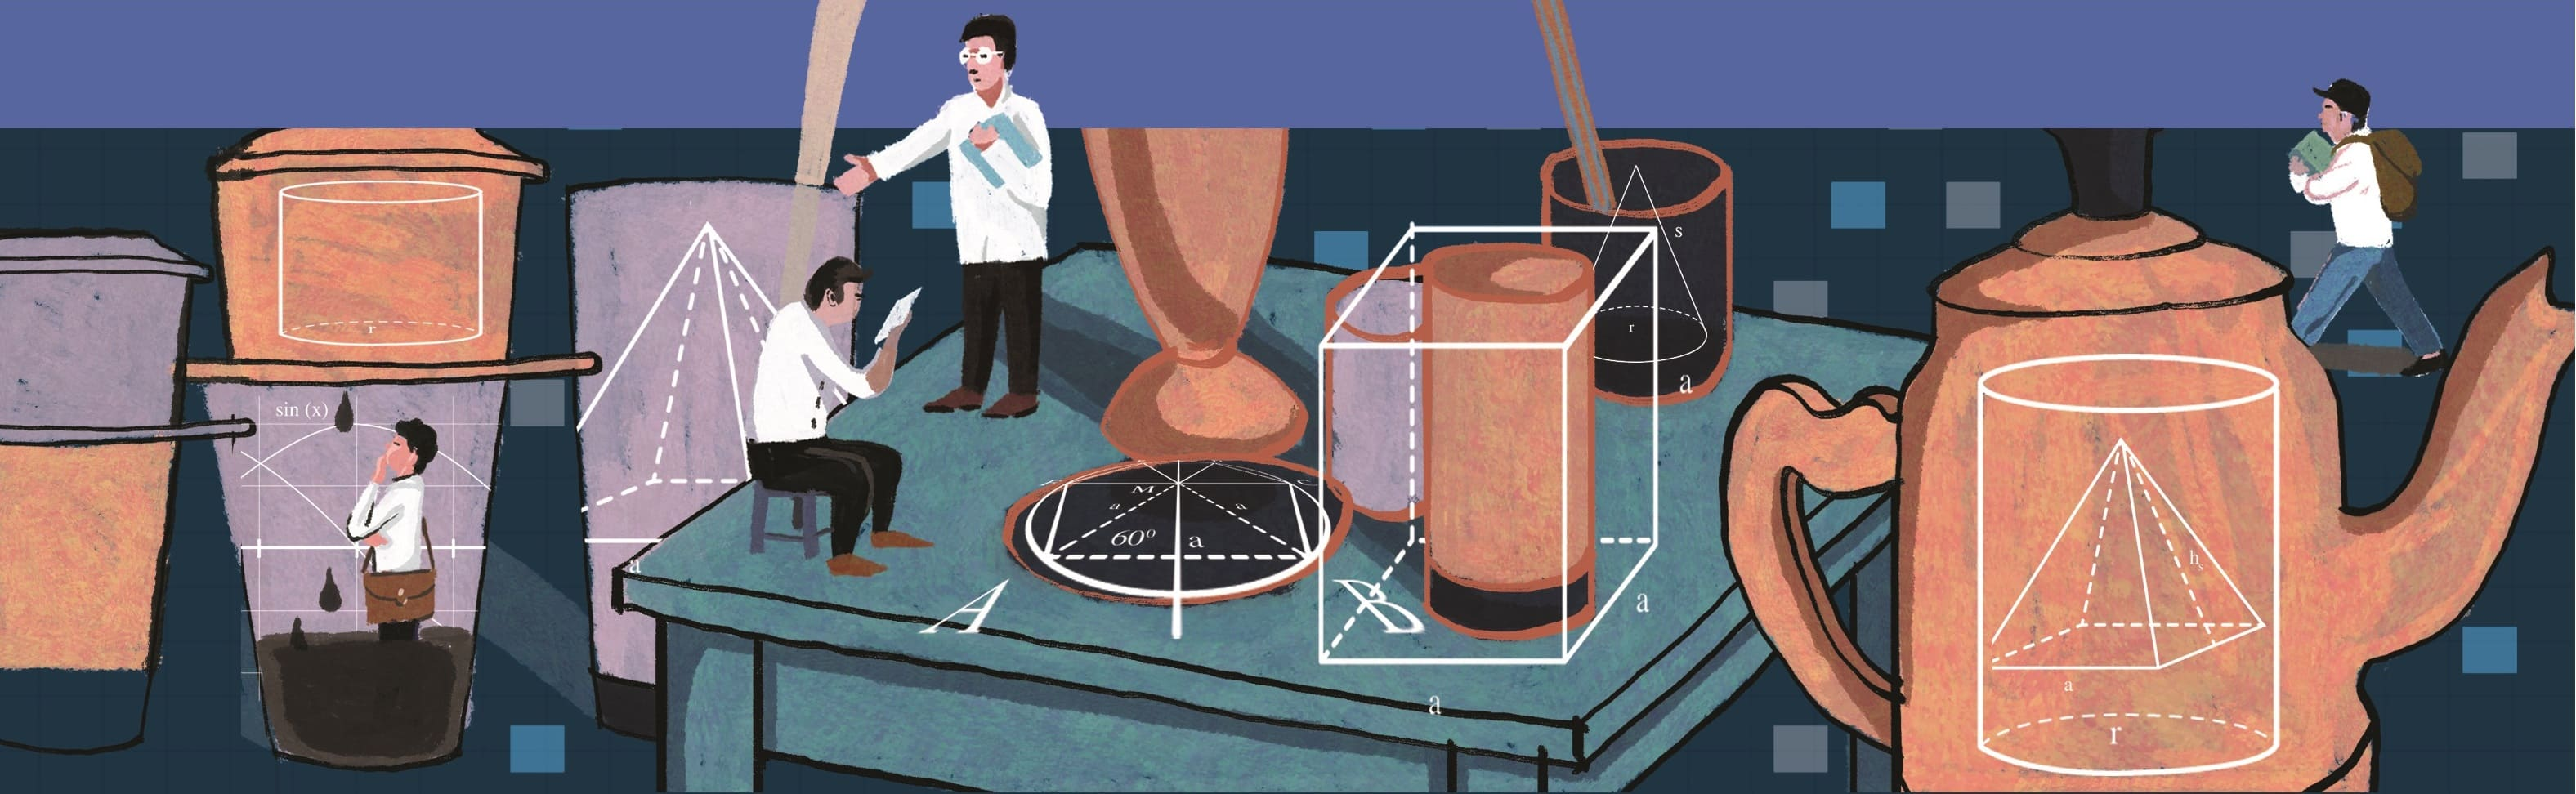
\includegraphics[width=19.3cm]{../bannerquantoan}}}
\AddToShipoutPicture*{\put(58,505){
\includegraphics[scale=1]{../tieude.pdf}}}
\centering
\endgroup

\vspace*{198pt}

\begin{multicols}{2}
	Ai cũng biết rằng Charles Lutwidge Dodgson (bút danh Lewis Carroll, $1832-1898$; Hình $1$), tác giả của \textit{Alice ở xứ xở diệu kỳ}, là một nhà toán học. Dodgson là một giảng viên toán tại trường Christ Church thuộc Đại học Oxford và đã có nhiều công trình toán học về hình học, đại số, logic và lý thuyết bỏ phiếu. Hầu hết mọi đánh giá về toán học của Dodgson đều nhắc đến một câu chuyện thú vị (sau đây gọi là \textit{câu chuyện}) liên quan đến nữ hoàng Victoria. Nữ hoàng được cho là rất thích truyện \textit{Alice}, xuất bản năm $1865$, và đã yêu cầu tác phẩm tiếp theo của tác giả. Với sự ngạc nhiên và thất vọng, bà đã nhận được cuốn \textit{Chuyên luận về định thức} của Dodgson, xuất bản năm $1867$. Câu chuyện này là một giai thoại kinh điển mà người ta thường bắt gặp trong các tác phẩm về toán học.
	\vskip 0.02cm
	Những bài viết về \textit{câu chuyện} cũng đôi khi nhắc nhở chúng ta rằng chính Dodgson đã phủ nhận nó vào năm $1896$, nhưng sự lan rộng của tin đồn dường như không thể ngăn được. Có thể dễ dàng hiểu được sức hấp dẫn của nó, vì nó thể hiện một cách hoàn hảo quan niệm rộng rãi về Dodgson nói riêng và toán học nói chung. Đầu tiên, câu chuyện truyền tải một cái nhìn rộng rãi về Dodgson như một nhân vật kép: một mặt là nhà toán học buồn tẻ và mặt khác là một tiểu thuyết gia giàu trí tưởng tượng. Thứ hai, phản ứng được cho là của nữ hoàng tiêu biểu cho niềm tin rằng toán học và văn học bắt nguồn từ những bộ óc và nền văn hóa khác nhau. Điều thú vị là nhiều lời kể về \textit{câu chuyện} nói rằng nữ hoàng không hài lòng khi nhận được cuốn sách. Người ta cũng nói rằng Dodgson, người rất tôn kính hoàng gia, không thể nào thực hiện một ``hành động hoàn toàn ngược với tính cách" như vậy (Beale $1973$). Nhưng  tặng một cuốn sách toán cho nữ hoàng thì có gì sai?  
	\begin{figure}[H]
		\vspace*{-5pt}
		\centering
		\captionsetup{labelformat= empty, justification=centering}
		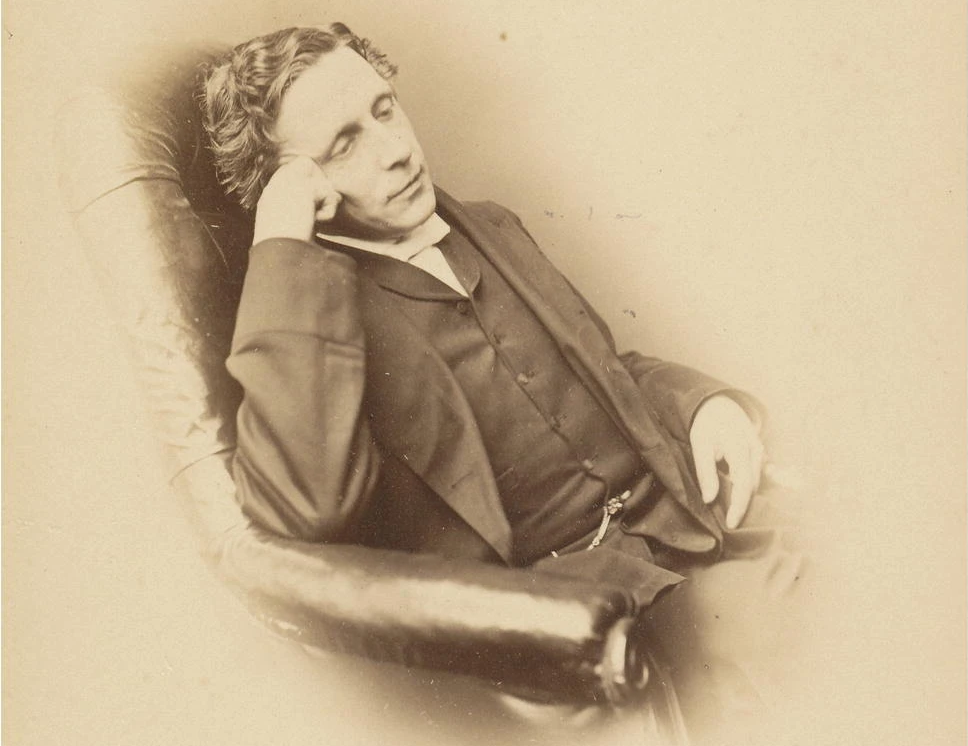
\includegraphics[width= 1\linewidth]{1}
		\caption{\small\textit{\color{quantoan}Hình $1$. Charles L. Dodgson (from the Wakeling
				Collection).}}
		\vspace*{-5pt}
	\end{figure}
	\textbf{\color{quantoan}Câu chuyện lan truyền chóng mặt}
	\vskip 0.1cm
	Khi \textit{Alice ở xứ xở diệu kỳ} ra mắt (Dodgson $1865$, Hình $2$), Dodgson là một tác giả vô danh. Ông mới chỉ xuất bản một số tập sách nhỏ về toán học và các tác phẩm nhỏ. Đặc biệt, vào năm $1856$, ông đã đóng góp một số bài thơ cho tạp chí \textit{Chuyến tàu}, ở đó ông sử dụng bút danh Lewis Carroll, lấy từ tên của mình (Lewis từ Lutwidge và Carroll từ Charles). Những năm sau đó, ông chủ yếu sử dụng tên thật cho các công trình toán học và bút danh cho các tác phẩm văn học để giữ kín danh tính của mình. Thành công tức thì của cuốn sách \textit{Alice} đã làm cho bút danh văn học của ông được đông đảo công chúng biết đến, nhưng họ không biết được ông có thể là ai.
	\begin{figure}[H]
		\vspace*{-5pt}
		\centering
		\captionsetup{labelformat= empty, justification=centering}
		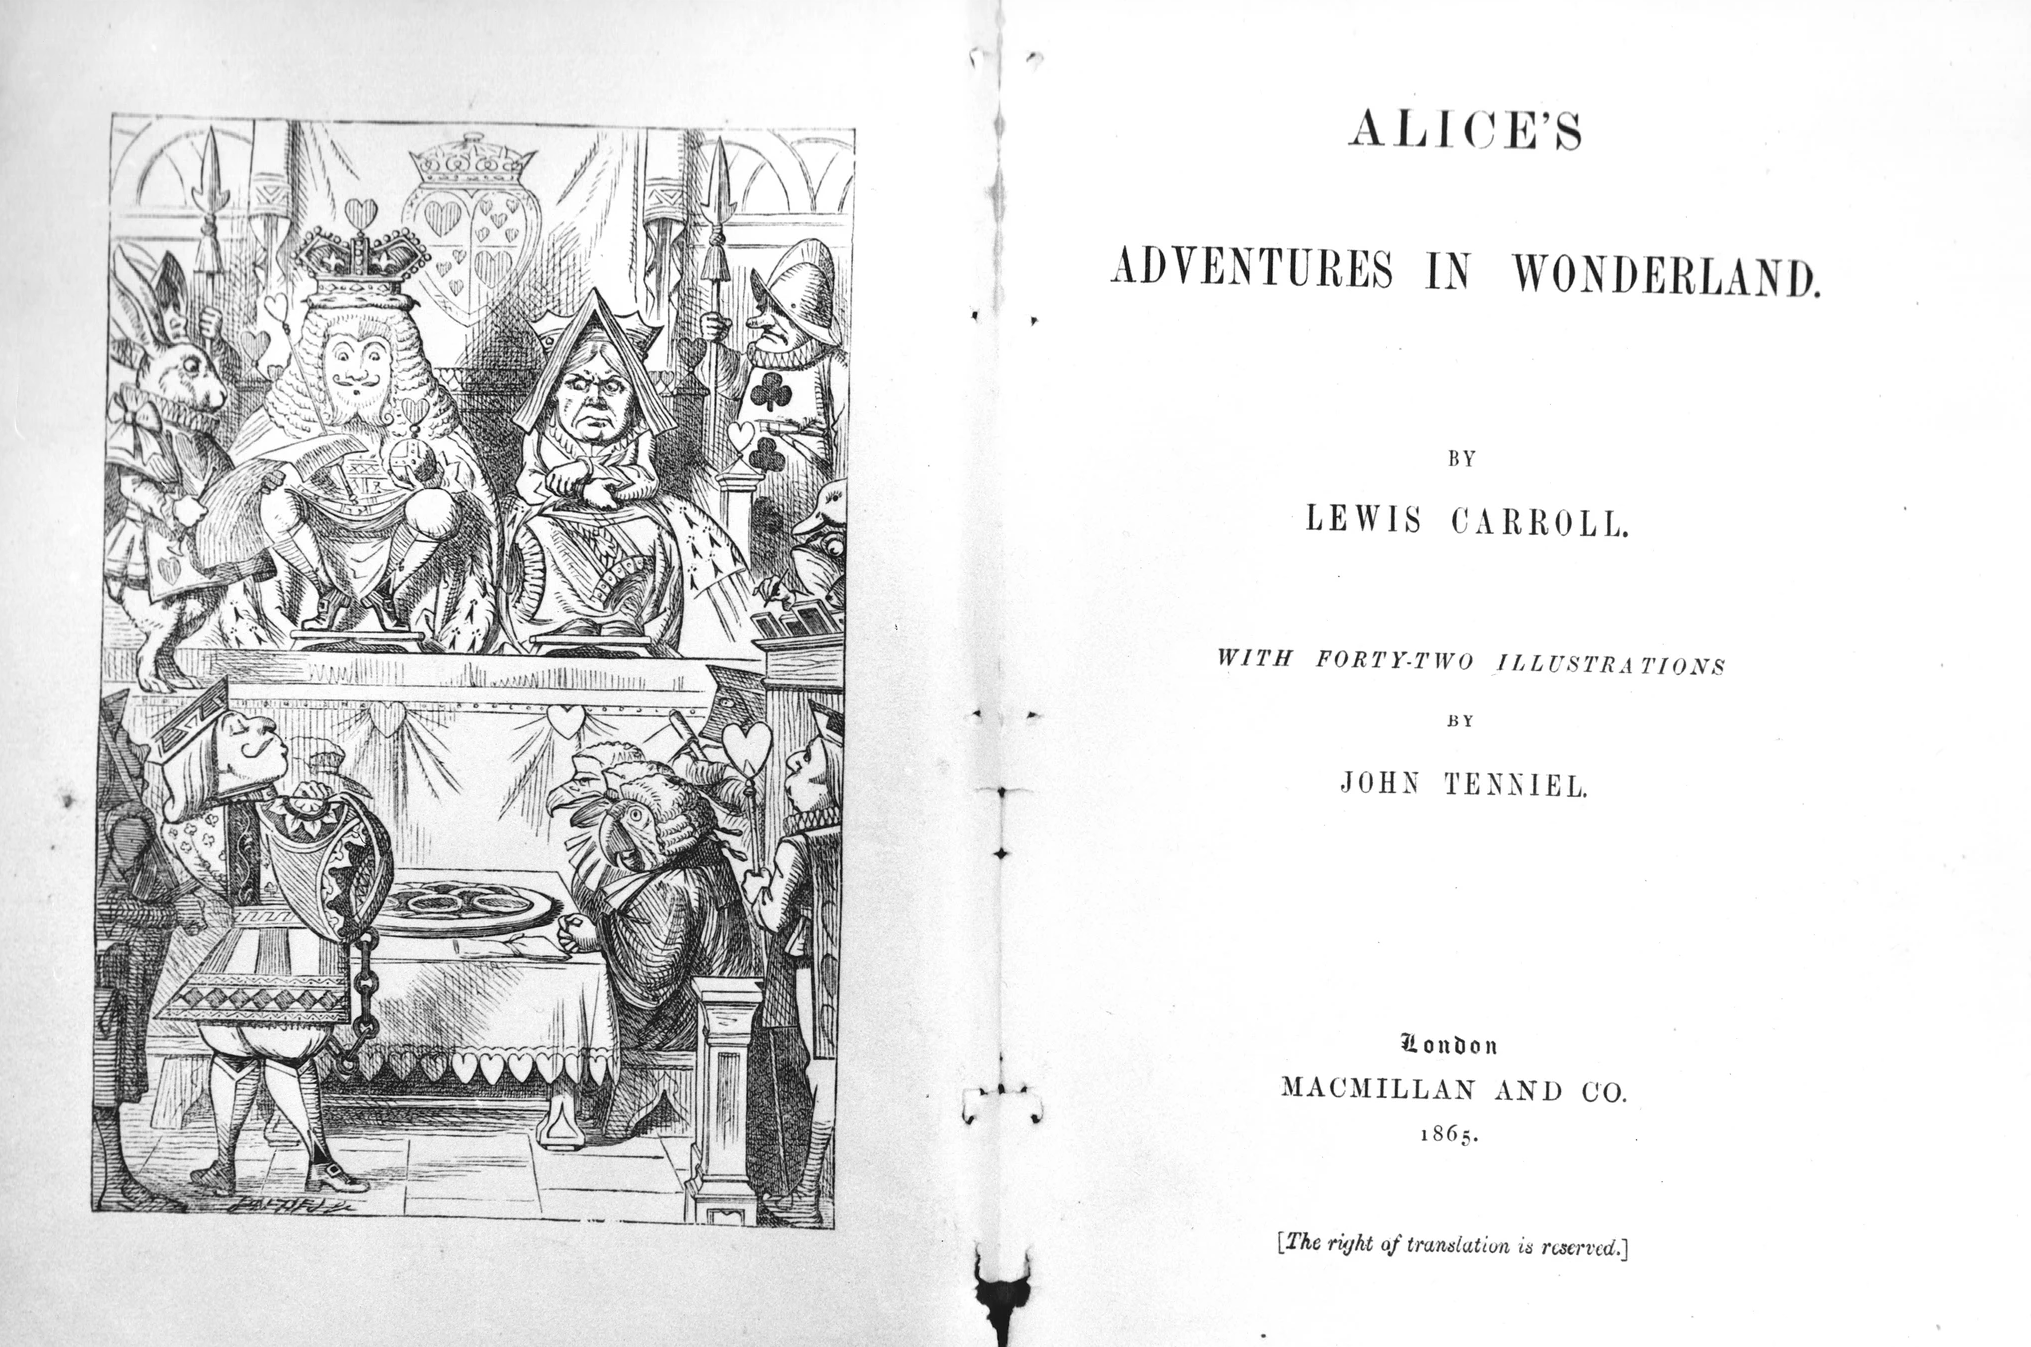
\includegraphics[width= 1\linewidth]{2}
		\caption{\small\textit{\color{quantoan}Hình $2$. The title page of Dodgson’s Alice’s Adventures in Wonderland, $1865$ (Photo by George Bayntun, Collection of Charlie Lovett).}}
		\vspace*{-10pt}
	\end{figure}
	Cuốn sách cũng được hưởng một nỗ lực quảng bá lớn của cả nhà xuất bản và tác giả. Vô số các bản sao đã được gửi đến các tạp chí để đánh giá, hoặc tặng bạn bè làm quà. Cháu trai, đồng thời là người viết tiểu sử đầu tiên của Dodgson, Stuart D. Collingwood, đã thuật lại rằng bản sao đầu tiên của cuốn sách được gửi đến Alice ngoài đời thực, người đã truyền cảm hứng cho câu chuyện, còn bản thứ hai được gửi đến công chúa Beatrice, con gái út của nữ hoàng Victoria (Collingwood $1898$, tr.$104$) . Đáp lại, Dodgson nhận được một lá thư cho biết ``cuốn sách nhỏ mà Bệ hạ rất hài lòng khi cho phép đọc nó cho công chúa Beatrice" (Wakeling $1999$, tr. $122$).
	\vskip 0.1cm
	Với sự khen ngợi của giới phê bình và số lượng lớn sách bán được, ý tưởng về phần tiếp theo hẳn đã nhanh chóng nảy ra với Dodgson và nhà xuất bản của ông. Ngay từ năm $1866$, Dodgson đã đề cập đến việc ``đang cân nhắc ý tưởng về việc viết một thứ kiểu như phần tiếp theo". Công chúng rõ ràng đã mơ màng về những cuộc phiêu lưu khác, và có tin đồn rằng ``Lewis Carroll đang viết tiếp" (Collingwood $1898$, tr.$129$).
	\vskip 0.1cm
	Quả thực là Dodgson đang viết. Bên cạnh những thứ khác, ông đang nghiên cứu về thứ có thể là đóng góp quan trọng nhất của ông cho nghiên cứu toán học. Thật vậy, ông đã đưa ra một phương pháp mới để tính toán các định thức, trình bày nó trước Hiệp hội Hoàng gia Luân Đôn vào tháng $5$ năm $1866$, và sau đó công trình này xuất hiện trong Kỷ yếu của Hiệp hội Hoàng gia Luân Đôn. Trong vòng một năm sau đó, Dodgson đã phát triển bài báo của mình thành một ``cuốn sách nhỏ", mà ông ghi lại trong nhật ký của mình là ``đã mang lại cho [ông] nhiều rắc rối hơn bất cứ thứ gì mà ông đã từng viết" (Wakeling $1999$, $206-207$). Việc xuất bản cuốn sách bị gián đoạn bởi một chuyến đi đến nước Nga cùng với Henry Parry Liddon từ tháng $7$ đến tháng $9$ năm $1867$. \textit{Chuyên luận về định thức} cuối cùng được xuất bản vào đầu tháng $12$ năm đó (Hình $3$). Cuốn sách này đã nhận được một số lời khen ngợi về đóng góp và tính mới, nhưng bị chỉ trích vì văn phong logic nặng nề và sự lựa chọn thuật ngữ và ký hiệu gây khó đọc.
	\vskip 0.1cm
	\textit{Chuyên luận về định thức} là cuốn sách đầu tiên của Dodgson kể từ Alice, nhưng nó không có liên hệ gì với cuốn truyện tuyệt vời đó. Trước khi hoàn thành, Dodgson đã thông báo cho nhà xuất bản của mình, Macmillan, trong một bức thư ngày $11$ tháng $2$ năm $1867$, về ý định đề tên thật của mình cho cuốn sách: ``Tôi có một cuốn sách nhỏ, sắp hoàn thành, mà tôi muốn các ông xuất bản cho tôi -- nhưng tôi e rằng nó không thể được giới thiệu như là của tác giả 'của \textit{Những cuộc phiêu lưu của Alice}'". Độc giả của chuyên luận chắc chắn không có lý do gì để nghi ngờ rằng tác giả của nó thực sự là người đã viết ra \textit{Alice}. Vào thời điểm đó, Dodgson đã giữ được bí mật danh tính của mình và chỉ tiết lộ nó cho một số bạn bè và những người quen may mắn. Những bức thư gửi cho Lewis Carroll được gửi đến nhà xuất bản Macmillan, sau đó nhà xuất bản chuyển tiếp tới ông dưới cái tên Charles L. Dodgson ở Oxford. Khi một cô bé yêu cầu ông viết một câu chuyện Alice khác vào năm $1867$, ông hồi âm dưới cái tên Dodgson, khẳng định rằng ông có một thông điệp cho cô ấy ``từ một người bạn ... ông Lewis Carroll, một sinh vật kỳ dị, khá thích nói những chuyện vô nghĩa".
	\begin{figure}[H]
		\vspace*{-5pt}
		\centering
		\captionsetup{labelformat= empty, justification=centering}
		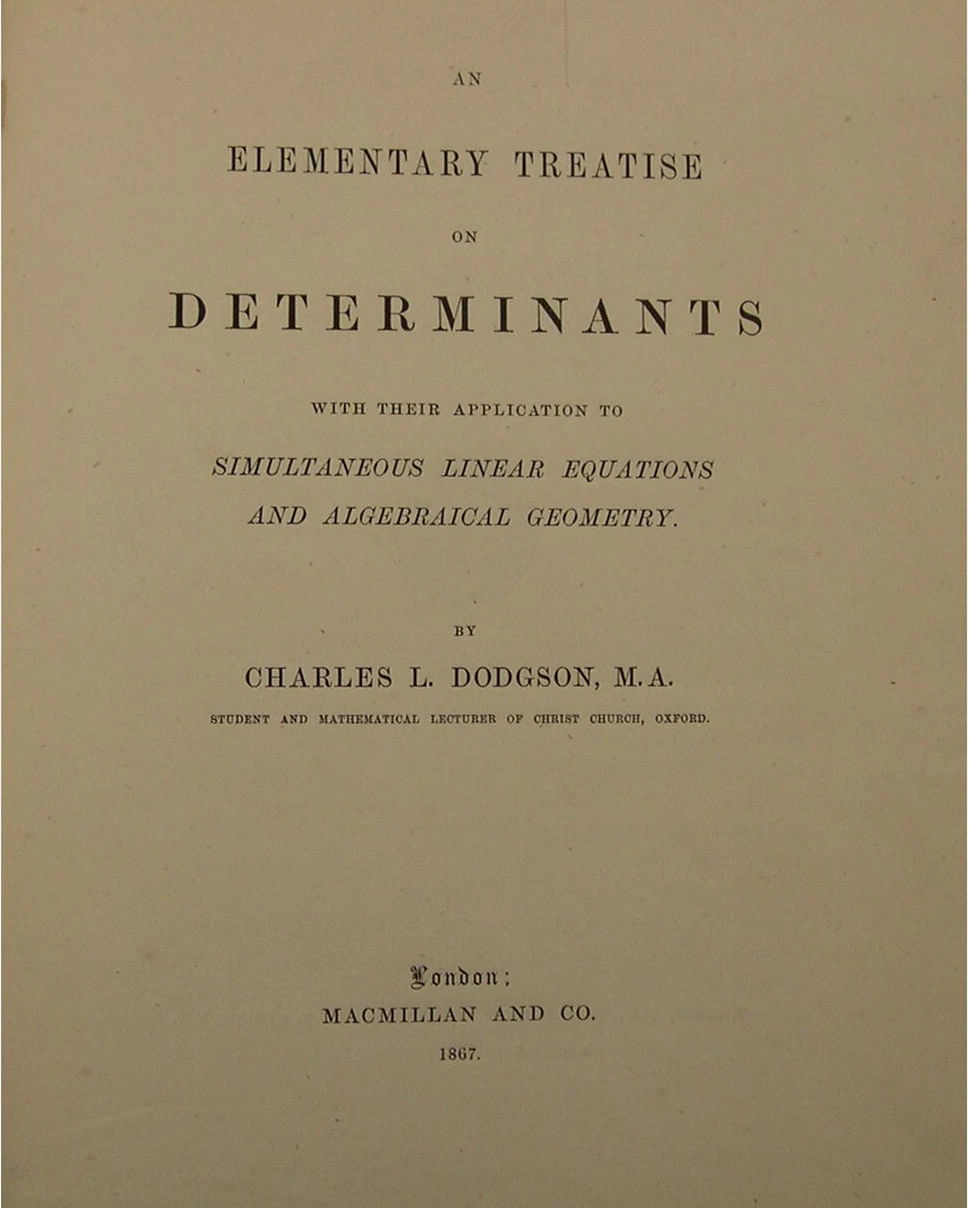
\includegraphics[width= 1\linewidth]{3}
		\caption{\small\textit{\color{quantoan}Hình $3$. The title page of Dodgson’s Elementary Treatise on Determinants, $1867$ (from the Wakeling Collection)}}
		\vspace*{-10pt}
	\end{figure}
	Khi \textit{Chuyên luận về định thức} ra mắt, có lẽ chỉ có một nhóm nhỏ độc giả có đặc quyền mới biết được bí mật nhỏ của tác giả, và ``nó là một phát hiện hoàn toàn bất ngờ với những sinh viên đại học lần đầu tiên được biết rằng ông Dodgson của trường Christ Church và Lewis Carroll chính là một" (Colingwood $1898$, tr.$110$). Một trong những người viết đánh giá về chuyên luận dường như biết điều đó, vì ông ta kết thúc bài đánh giá của mình bằng cách hy vọng ``có thêm khảo sát về thế giới thần tiên đại số tùy chọn [của tác giả]". Sự ám chỉ này đến truyện \textit{Alice} chắc hẳn đã khiến Dodgson khó chịu, một người đã rất cố gắng giữ bí mật về danh tính của mình. Dodgson phàn nàn trong một bức thư gửi cho chị dâu của mình, vào ngày $31$ tháng $7$ năm $1890$, rằng ông thấy khá kỳ lạ rằng ``mọi người sẽ không hiểu rằng, khi một tác giả sử dụng \textit{bút danh}, thì mục đích là \textit{tránh} việc công khai danh tính cá nhân, điều mà họ luôn cố gắng thúc giục anh ta". Có vẻ như việc Dodgson nhất quyết giữ bí mật danh tính của mình chỉ khiến những ``kẻ săn đuổi" ông trở nên đông đảo và quyết tâm hơn. Quả là tình huống đó hẳn đã gợi nên sự tò mò và hấp dẫn, và dễ dàng hình dung được sự ngạc nhiên của một độc giả nhiệt tình của \textit{Alice}, không biết rằng tác giả của nó là một giảng viên toán tại Oxford, khi đối diện với cuốn sách tiếp theo của tác giả, về chủ đề định thức, và được cho biết tác giả thực sự là ai. Những gì đã có thể là một giai thoại thú vị đã trở thành một câu chuyện lan truyền chóng mặt khi độc giả bối rối tình cờ lại chính là nữ hoàng.
	\vskip 0.1cm
	Câu chuyện này quá hay và không khó để có thể là sự thật. Thực sự là nữ hoàng biết, và có thể rất thích truyện \textit{Alice}. Bà  chỉ cần hỏi, và có thể bà ấy đã hỏi, về cuốn sách tiếp theo của tác giả, để khiến cho \textit{câu chuyện} xảy ra. Đó là một \textit{câu chuyện} tuyệt vời, và sẽ còn tuyệt vời hơn nếu Dodgson không hoàn toàn phủ nhận nó, gần ba mươi năm sau thời điểm mà nó được cho là đã xảy ra.
	\vskip 0.1cm
	\textbf{\color{quantoan}Phủ nhận} 
	\vskip 0.1cm
	Đến năm $1896$, Dodgson là một tác giả nổi tiếng từ chối tận hưởng danh tiếng của mình. Phần tiếp theo của câu chuyện, \textit{Đi qua tấm gương}, cũng  thành công như truyện \textit{Alice ở xứ sở diệu kỳ}.
	\vskip 0.1cm
	Sau đó, ông xuất bản nhiều tác phẩm hư cấu khác, nhưng không có tác phẩm nào thực sự sánh được với hai truyện \textit{Alice}. Là một nhà toán học, ông cũng đã xuất bản nhiều về nhiều chủ đề khác nhau, đặc biệt là bảo vệ một cách đẹp đẽ hình học Euclid trước những sách giáo khoa mới muốn thay thế nó trong các trường trung học và đại học. Trong những năm cuối đời, ông viết một chuyên luận về logic nhằm giúp chủ đề này có thể tiếp cận tới một công chúng rộng rãi. Không giống như các đồng nghiệp của mình tại Đại học Oxford, Dodgson đã chấp nhận lý thuyết logic hình thức mới được phát triển ở Anh bởi George Boole và những người theo trường phái của ông. Phần đầu tiên của chuyên luận của Dodgson, \textit{Logic hình thức}, xuất bản vào tháng $2$ năm $1896$. Lần tái bản thứ nhất, ra mắt vào đầu tháng $6$ cùng năm, có lời tựa được đề ngày $11$ tháng $5$ năm $1896$ (Hình $4$). Ngoài một vài thay đổi và sửa chữa nhỏ, nó có một phần tái bút sau trang tiêu đề, với ghi chú sau:
	\vskip 0.1cm
	\textit{Tôi xin nhân cơ hội này để phủ nhận một cách công khai nhất  có thể  một câu chuyện ngớ ngẩn, được lan truyền trên báo chí, về việc tôi đã tặng một số cuốn sách nào đó cho Nữ hoàng. Nó được lặp đi lặp lại liên tục, và là thêu dệt hoàn toàn, đến nỗi tôi nghĩ rằng đáng để tuyên bố, một lần dứt điểm, rằng nó tuyệt đối sai trong mọi chi tiết: không có bất kỳ điều gì thậm chí hơi giống như thế đã từng xảy ra cả.}
	\vskip 0.1cm
	Dodgson đã giữ ghi chú này trong lần tái bản thứ hai của cuốn sách, có lời tựa đề ngày $20$ tháng $7$ năm $1896$, nhưng vì lý do nào đó đã bỏ nó khỏi lần tái bản thứ ba, xuất bản vào đầu năm $1897$ nhưng có lời tựa vào Giáng sinh năm $1896$.
	\vskip 0.1cm
	Trong ghi chú này, Dodgson đã mạnh mẽ phủ nhận một ``câu chuyện ngớ ngẩn" về việc ông đã tặng một số cuốn sách cho nữ hoàng. Có thể lưu ý rằng giải thích của Dodgson là rất ít ỏi và có thể đề cập đến một sự việc khác, nhưng có vẻ như chỉ đơn giản là ông không muốn kể chi tiết về giai thoại để không quảng bá thêm về nó. Dodgson rõ ràng không thấy thích thú gì với \textit{câu chuyện}. Vì tin đồn đề cập đến các sự kiện được cho là diễn ra vào năm $1867$, một số tác giả tự hỏi tại sao Dodgson phải mất gần ba mươi năm để phủ nhận nó (Wakeling $2015$, tr. $315$). Derek Hudson cho rằng Dodgson có thể đã dùng thời gian này để tranh luận ``với chính bản thân mình liệu có đúng khi phản bác câu chuyện hay không (Hudson $1976$,  tr.$133$). Một lời giải thích hợp lý hơn có thể là Dodgson chỉ đơn giản là phủ nhận câu chuyện khi nó được lan truyền rộng ra, vì không có lý do gì để cho rằng tin đồn được bắt đầu trong cùng thời kỳ mà những sự việc được kể lại trong \textit{câu chuyện} được cho là đã xảy ra.
	\begin{figure}[H]
		\vspace*{-5pt}
		\centering
		\captionsetup{labelformat= empty, justification=centering}
		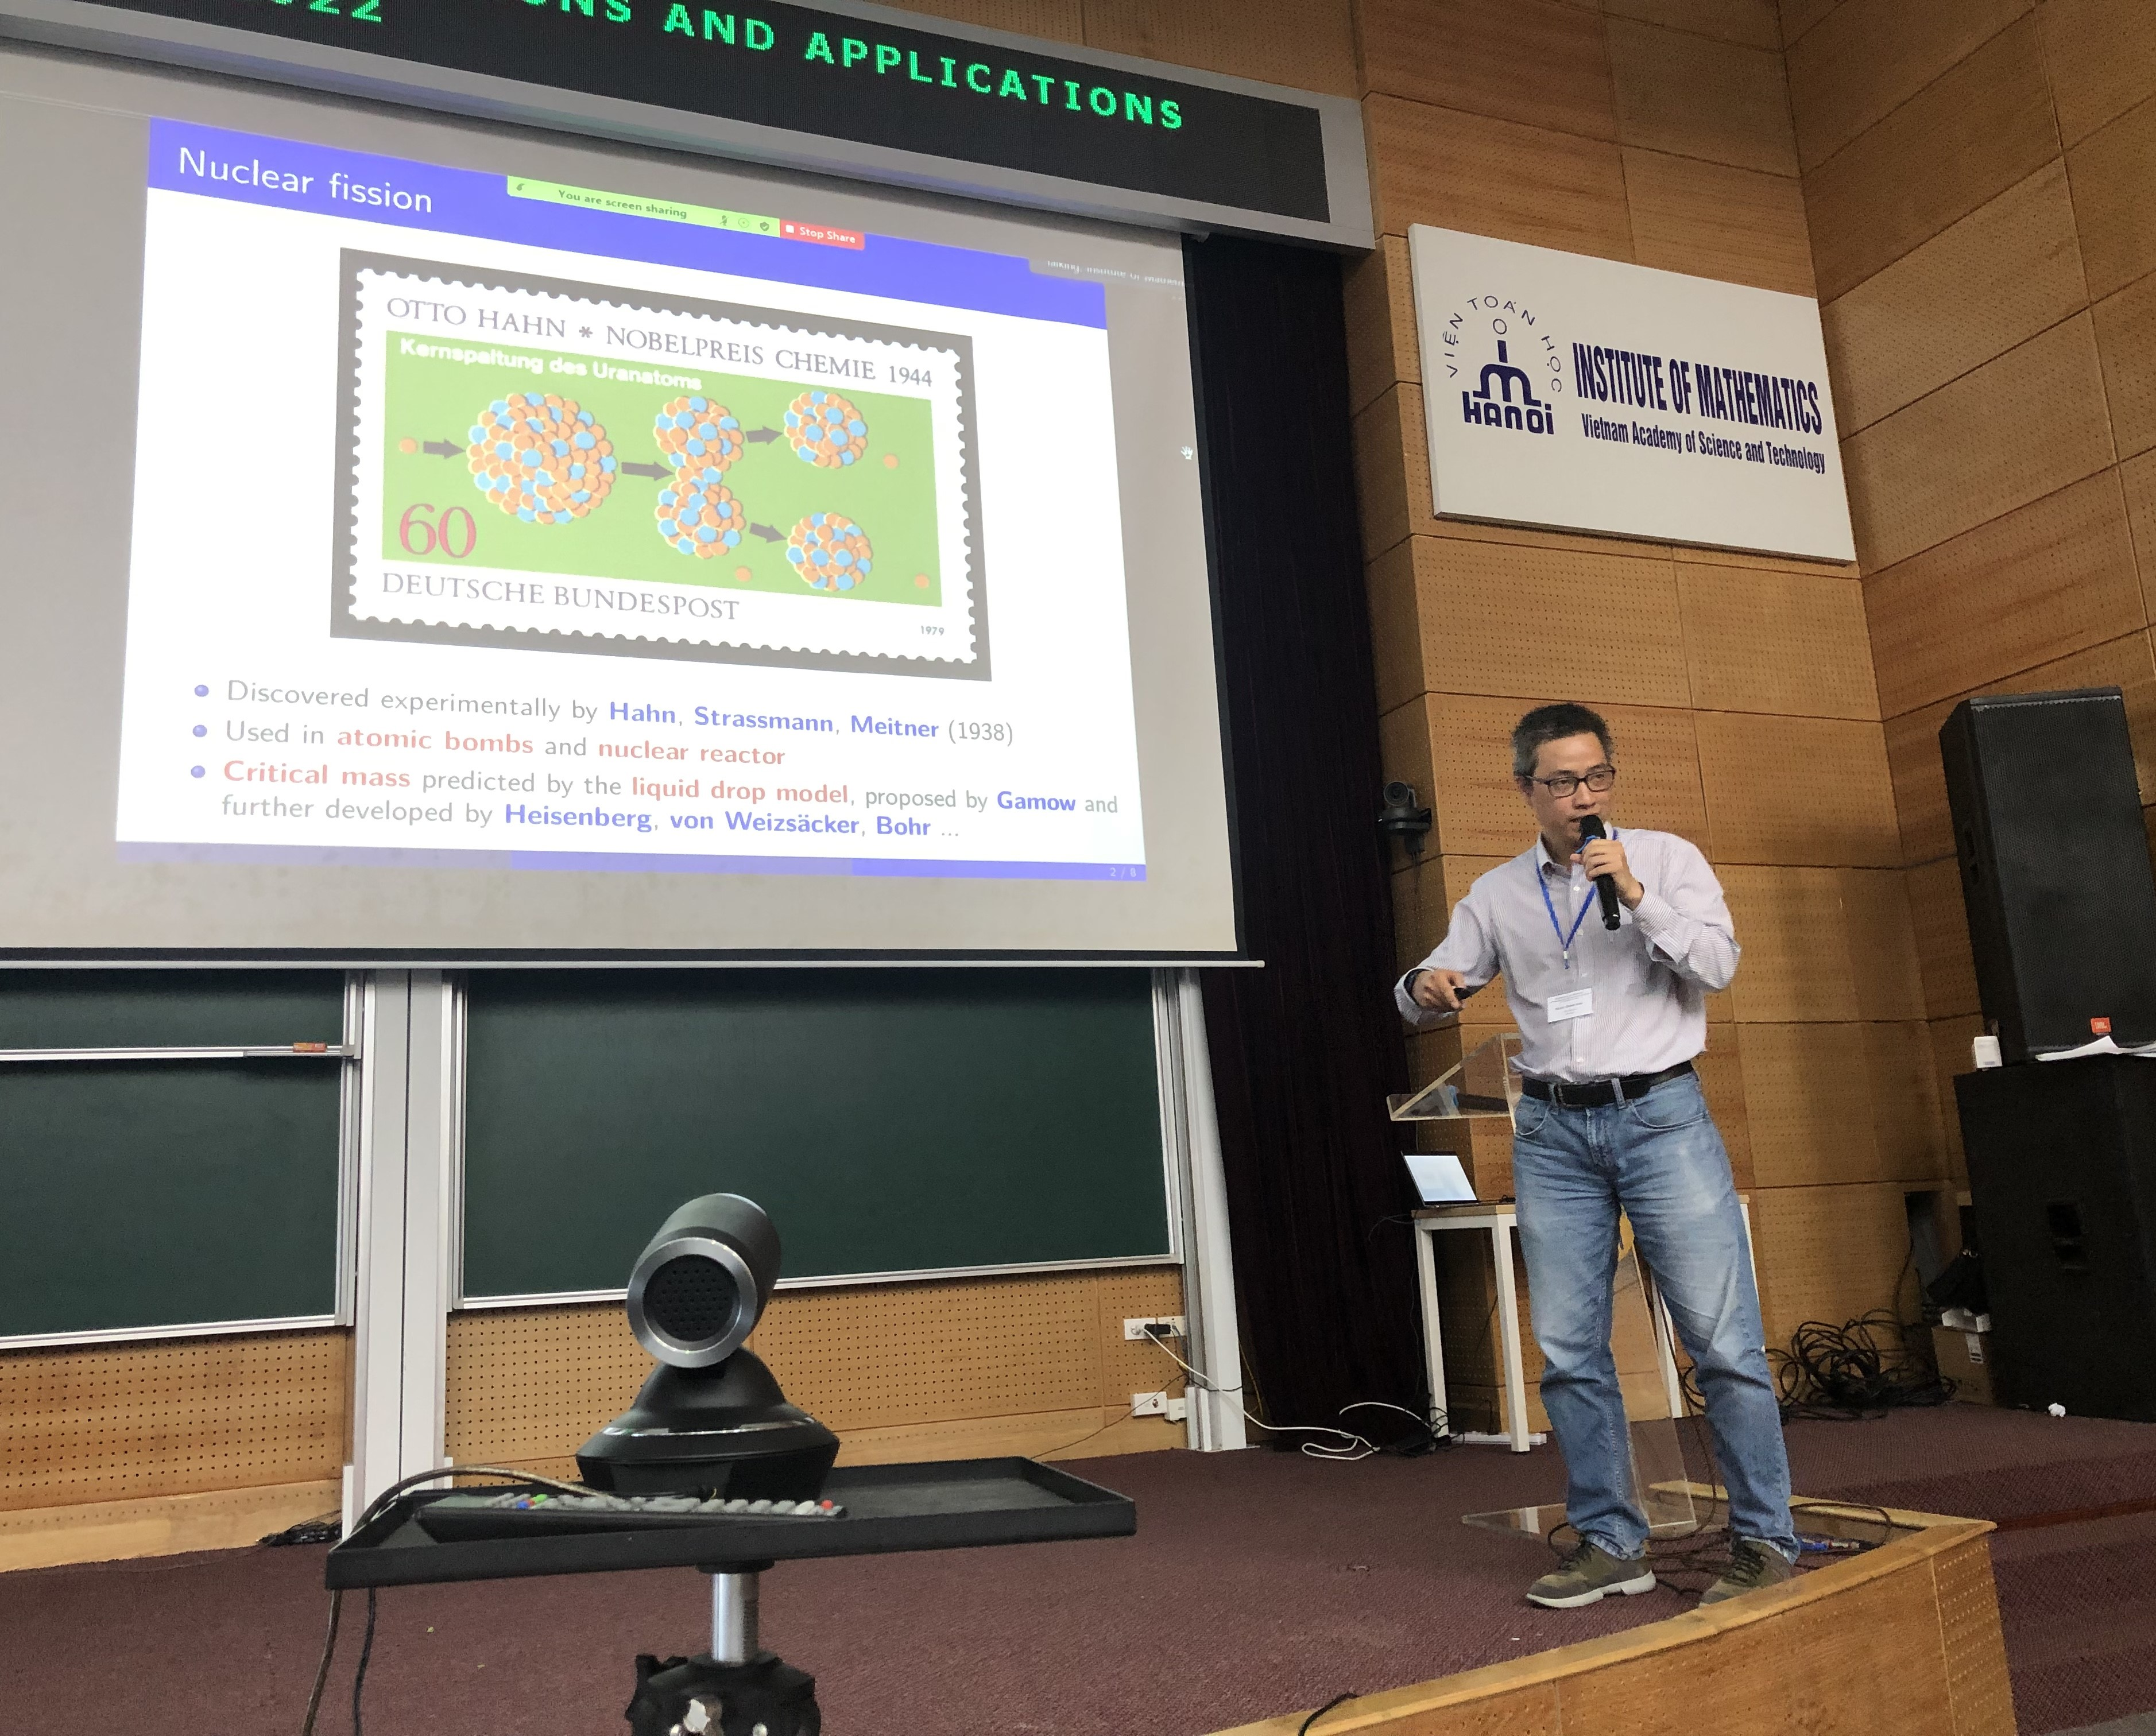
\includegraphics[width= 1\linewidth]{4}
		\caption{\small\textit{\color{quantoan}Hình $4$. The title page of Dodgson’s Symbolic Logic, second edition, $1896$, and the Advertisement page, which includes a denial of the story (from the Wakeling Collection).}}
		\vspace*{-10pt}
	\end{figure}
	Trên thực tế, có vẻ như không biết tin đồn đã bắt đầu từ khi nào. Trong một thời gian dài, người ta thậm chí đã nghĩ rằng không có bằng chứng văn bản nào về sự tồn tại của tin đồn trước sự phủ nhận của chính Dodgson vào năm $1896$. Tuy nhiên, trong những năm gần đây, một số bài báo trước đó về nó đã được tìm thấy, và giờ đây mọi thứ trở nên rõ ràng rằng tin đồn đã lan truyền khá rộng vào quãng thời gian mà Dodgson phủ nhận nó. Tin đồn chắc chắn tồn tại ít nhất từ năm $1892$, vì nó được tìm thấy trên một số tờ báo thời đó, chẳng hạn như \textit{Sporting Times}. Nó dường như đã được lan truyền rộng rãi hơn sau năm $1895$, đặc biệt là sau khi nó được Ethel Mackenzie McKenna kể lại trong số tháng $8$ năm $1895$ của \textit{Tạp chí Ladies’ Home}:
	\vskip 0.1cm
	``Trong thời kỳ  mới mẻ của sự thành công rực rỡ, ``Alice" nằm  trên tay của mọi người và những chuyến phiêu lưu vào thế giới thần tiên của cô là niềm vui thích của  người lớn cũng như trẻ em. Nữ hoàng Victoria đã gửi một thông điệp đến tác giả, xin ông gửi cho bà cuốn sách tiếp theo của mình. Giống như tất cả các thần dân của mình, bà nóng lòng muốn nghe nhiều hơn về đứa trẻ thú vị, mà nguyên mẫu là con gái của hiệu trưởng của trường Christ Church. Bà đã rất kinh ngạc khi không lâu sau đó nhận được một cuốn ``\textit{Chuyên luận về định thức}" của C. L. Dodgson, vì khi đó, ông vẫn giữ bí mật về danh tính của mình, và Nữ hoàng, cũng như cả thế giới, đã tin rằng ông chỉ đơn thuần là một người hài hước."
	\vskip 0.1cm
	Tạp chí của Mỹ này có lượng độc giả rộng lớn và ngày càng tăng vào thời Dodgson, và vào năm $1904$, nó trở thành tạp chí đầu tiên đạt được số lượng một triệu người đặt báo. Lời kể của McKenna về \textit{câu chuyện} được đăng lại trên các tạp chí khác của Mỹ, nhất là trong các mục tin đồn, tin vắn và tin tức văn học. \textit{Câu chuyện} hẳn cũng đã lan tới một số tờ báo của Anh, vì nó được đăng trên tờ \textit{Newcastle Weekly Courant}. Đúng là \textit{câu chuyện} không được tìm thấy trên các tờ báo lớn của Anh, một sự thật có thể được giải thích là do họ không muốn xuất bản những bài viết tiết lộ danh tính của Dodgson. Được biết, Dodgson không hài lòng với những bài viết như vậy và đã liên tục viết thư phàn nàn đến những tạp chí và nhà xuất bản của Anh đã tiết lộ hoặc muốn tiết lộ tên thật đằng sau bút danh của ông. Các tạp chí nước ngoài hiển nhiên nằm ngoài tầm ảnh hưởng của Dodgson, như ông thừa nhận trong một bức thư gửi cho Falconer Madan vào ngày $8$ tháng $12$ năm $1880$: ``Tôi e rằng các ấn phẩm của Mỹ nằm ngoài tầm khiếu nại của các nhà văn Anh: chỉ ở Anh, người ta mới có thể hy vọng ngăn tên mình được công bố."
	\vskip 0.1cm
	Vào năm $1895$, \textit{câu chuyện} rõ ràng là đã ``lan truyền trên báo chí" và được ``lặp đi lặp lại liên tục", như Dodgson đã viết trong lời phủ nhận của mình. Người ta lập luận rằng ``không chắc Dodgson đã xem tạp chí [\textit{Tạp chí Ladies’ Home}] này" (Wakeling $2005$, tr. $257$); tuy nhiên, ông có thể đã thấy một trích dẫn về nó được đăng lại trên các tờ báo của Anh. Chúng ta cũng biết rằng Edward Bok, chủ bút của \textit{Tạp chí Ladies’ Home}, đã đến thăm Dodgson ở Oxford để thuyết phục ông đóng góp bài cho tạp chí. Chuyến thăm này được ghi lại trong tự truyện của Bok, nhưng ngày tháng không được nêu rõ ràng. Tuy nhiên, lời kể đó gợi ý rằng nó trùng hợp với lần Bok đến thăm Rudyard Kipling, người đã được thuyết phục đóng góp câu chuyện ``William the Conqueror" của mình cho tạp chí. Do câu chuyện của Kipling xuất bản vào cuối năm $1895$, sẽ khá hợp lý khi cho rằng chuyến thăm diễn ra trước đó. Điều thú vị là Bok kể về việc ông đã hỏi Dodgson về câu chuyện gửi tặng cuốn sách \textit{Chuyên luận về định thức} cho nữ hoàng, một câu hỏi mà Dodgson  không bình luận, nhưng ``khuôn mặt của ông ấy hoàn toàn không có biểu hiện gì ngoài vẻ trắc ẩn nhằm nói với người chủ bút rằng ông ta đang mắc một sai lầm khủng khiếp" (Bok $1920$, tr. $222-223$). Trước sự thất vọng lớn của Bok, Dodgson chỉ đơn giản  phủ nhận việc mình là tác giả của hai cuốn sách \textit{Alice}. Nếu lời kể của Bok là sự thật, ông ta đã sớm được chứng kiến Dodgson bác bỏ câu chuyện, trước khi ông phủ nhận bằng văn bản, trong cuốn sách. Nhưng chúng ta có nên tin Dodgson không?
	\vskip 0.1cm
	\textbf{\color{quantoan}Liệu rằng nó đã xảy ra?}
	\vskip 0.1cm
	Việc tìm hiểu sự thật về \textit{câu chuyện} có vẻ là việc làm kỳ quái và thiếu tôn trọng bởi vì Dodgson đã phủ nhận nó một cách rõ ràng. Tuy nhiên, chúng ta không được quên rằng Dodgson thường xuyên phủ nhận (một cách không đúng) rằng ông là tác giả của  \textit{Alice}, vì vậy chúng ta không có thêm lý do gì để tin vào sự thật của lời phủ nhận này so với tất cả những lời phủ nhận khác mà chúng ta biết là không đúng. Câu chuyện của chúng ta kết nối tác giả của \textit{Alice} với tác giả của \textit{Chuyên luận về định thức}. Dodgson không có lựa chọn nào khác ngoài việc phủ nhận nó, bất kể sự thật là gì, nếu ông ấy muốn -- và chúng ta biết rằng ông thực sự muốn -- giữ bí mật về danh tính của mình.
	\vskip 0.1cm
	Chúng ta hầu như không thể nhấn mạnh đủ mức độ quan trọng của việc giữ kín danh tính đối với Dodgson. Các tiểu sử về ông chứa nhiều mẩu chuyện về việc ông từ chối là tác giả của truyện \textit{Alice} khi được hỏi về nó. Dodgson cũng từ chối lời mời tham dự các buổi chiêu đãi do nhà xuất bản của ông tổ chức, nơi ``hầu như không thể giữ được sự ẩn danh". Khi những lá thư được gửi đến trường Christ Church cho ông dưới cái tên Lewis Carroll , ông  đã gửi trả lại chúng mà không mở. Năm $1890$, ông thậm chí còn ban hành một thông cáo để gửi cho những người đã gửi thư đến như sau:
	\vskip 0.1cm
	``Ông Dodgson thường xuyên bị những người lạ gửi thư đến với giả định khá trái phép rằng ông tuyên bố, hoặc trong một chừng mực nào đó thừa nhận quyền tác giả của những cuốn sách không được xuất bản dưới tên ông, đến mức ông thấy cần phải tuyên bố điều này, một lần dứt điểm, như một câu trả lời cho tất cả các bức thư như vậy. Ông ta không tuyên bố hay thừa nhận bất kỳ mối liên hệ nào với bất kỳ bút danh nào, hoặc với bất kỳ cuốn sách nào không được xuất bản dưới tên của chính ông ta. Do đó, không có quyền giữ lại, hoặc thậm chí đọc thư bên trong, ông ta gửi trả lại nó cho người viết thư đã viết sai địa chỉ."
	\vskip 0.1cm
	Lưu ý rằng Dodgson không chính thức phủ nhận là tác giả của các truyệnAlice trong thông cáo này; ông chỉ đơn thuần từ chối việc đòi hoặc thừa nhận quyền tác giả đó. Nhưng Lloyd Humberstone khuyến cáo một cách đúng đắn rằng
	``Chúng ta không nên coi trọng những lời phủ nhận [của Dodgson] hơn những lời phủ nhận của một nghi phạm bị bắt trong cuộc truy tìm Jack the Ripper của cảnh sát, người khẳng định rằng anh ta không muốn được biết đến với cái tên đó, rằng anh ta không tuyên bố -- hay thừa nhận -- đã thực hiện bất kỳ vụ giết người nào, v.v." (Humberstone $1995$, tr. $498$).
	\vskip 0.1cm
	Đúng là bí mật về danh tính của Dodgson dần dần được hé lộ và có lẽ nó đã trở thành một bí mật công khai vào những năm cuối đời của ông. Các tờ báo thỉnh thoảng có đề cập đến danh tính của ông, và từ điển các bút danh thường liệt kê ông. Khá hợp lý khi cho rằng bí mật có lẽ được lan truyền qua số đông bạn bè và người quen của ông. Tuy nhiên, Dodgson vẫn từ chối thừa nhận là tác giả của những truyện \textit{Alice} khi những người lạ tiếp cận ông hoặc viết thư cho ông về nó. Những nỗ lực nhiệt thành của Dodgson để bảo vệ bí mật của mình,  thậm chí ngay cả sau này khi danh tính của ông đã được biết đến rộng rãi, hẳn đã khiến những người cùng thời của ông phải tò mò. Các cuốn tiểu sử về ông thuật lại cái cách mà trong suốt cuộc đời của mình, ông ấy là ``\textit{mục tiêu thường xuyên của những lời đồn đại}".
	\vskip 0.1cm
	Việc phủ nhận \textit{câu chuyện} của Dodgson cần phải được hiểu trong bối cảnh này: \textit{câu chuyện} chỉ là một trong số rất nhiều tin đồn về tác giả của \textit{Alice} và sự phủ nhận chỉ là một trong số rất nhiều tình huống mà Dodgson cố gắng giữ bí mật danh tính của mình. Tuy nhiên, có một nét nổi bật về việc Dodgson phủ nhận \textit{câu chuyện} trong cuốn \textit{Logic Hình thức} của ông. Dodgson tin tưởng vào lợi ích xã hội của logic hình thức và muốn cuốn sách của mình dễ tiếp cận đối với rộng rãi độc giả. Để quảng bá rộng rãi hơn cho cuốn sách chuyên luận  của mình, ông đã dùng bút danh văn học của mình thay vì tên thật, vốn thường được sử dụng cho các công trình toán học. Vì vậy, lời phủ nhận mà ông  đưa vào chuyên luận có thể là dịp duy nhất mà Dodgson, dưới cái tên Lewis Carroll, phủ nhận mối liên hệ của ông với Charles L. Dodgson.
	\vskip 0.1cm
	Chúng tôi đã nói ở trên rằng \textit{câu chuyện} thực sự không khó để có thể là  thật. Thật vậy, có những lý do chính đáng để tin rằng \textit{câu chuyện} đã thực sự xảy ra, và người ta sẽ không ngạc nhiên nếu nó đã xảy ra. Tuy nhiên, Thomas B. Strong, một người bạn của Dodgson, trong hồi ký viết năm $1932$, đưa ra hai lý do để không tin vào điều đó:
	\vskip 0.1cm
	``Thật trái ngược với toàn bộ thái độ của Dodgson đối với Hoàng gia và với cung cách đúng mực của ông ấy nếu  ông ấy giễu cợt Nữ hoàng như vậy. Và nó hoàn toàn trái ngược với thái độ của ông ấy đối với những cuốn sách của mình. Ông ấy luôn từ chối thừa nhận với bất kỳ người nào, ngoại trừ một số những người có đặc quyền đặc biệt, rằng ông ấy là Lewis Carroll."
	\vskip 0.1cm
	Có vẻ như Strong không nhận thấy rằng hai lý do ông ấy đưa ra có phần trái ngược nhau. Thật vậy, Dodgson hoặc phải gửi cuốn sách tiếp theo của mình, và do đó tiết lộ danh tính của ông, hoặc từ chối gửi nó, và do đó từ chối yêu cầu của nữ hoàng, mặc dù ông có thể đã  lập luận rằng cuốn sách tiếp theo của Lewis Carroll hoàn toàn không phải là cuốn sách tiếp theo của Charles Dodgson.
	\vskip 0.1cm
	Lưu ý rằng lý do đầu tiên mà Strong đưa ra cho thấy rằng việc Dodgson gửi tặng một cuốn sách toán cho nữ hoàng là điều đáng hổ thẹn và thô lỗ. Nhưng lý do thứ hai có vẻ như không đúng, vì chúng ta có thể tưởng tượng Dodgson hẳn sẽ vui vẻ coi nữ hoàng là một trong số ``những người có đặc quyền" được ông đã tiết lộ danh tính của mình, và chắc chắn ông đã tiết lộ điều đó để được giao thiệp với một số nhân vật nổi tiếng cùng thời.
	\vskip 0.1cm
	Dodgson không đáng tin cậy lắm khi ông phủ nhận những \textit{câu chuyện} tiết lộ danh tính của mình; thậm chí chỉ cần nhìn qua danh sách những phủ nhận của ông là đủ để ủng hộ việc không tin vào ông. Nhưng có thể có một lý do chính đáng để tin Dodgson một lần. Thật vậy, việc Dodgson phủ nhận \textit{câu chuyện} sẽ không ảnh hưởng đến niềm tin của chúng ta về nó nếu nhân vật liên quan không phải là nữ hoàng. Tôi không tin rằng việc tặng một cuốn sách toán học cho nữ hoàng sẽ đi ngược lại cách hành xử đúng mực của Dodgson. Tuy nhiên, việc công khai phủ nhận một câu chuyện liên quan đến nữ hoàng, câu chuyện có thể sẽ được nữ hoàng công nhận là thật, có thể sẽ bị coi là đáng hổ thẹn đối với một thần dân thời Victoria, một người ``yêu nước nồng nàn và là một tín đồ trung thành của những hoạt động của hoàng gia" (Hudson $1976$, $133$).
	\vskip 0.1cm
	Được biết, Dodgson rất kính trọng nữ hoàng và hoàng gia. Trong suốt cuộc đời mình, ông đã có một số dịp gặp gỡ các thành viên của hoàng gia, và ông chắc chắn đã quen với một số người trong họ. Ông đã tường thuật chi tiếttrong nhật ký của mình chuyến thăm trường Christ Church của nữ hoàng, vào tháng $12$ năm $1860$. Trong các chuyến thăm Oxford của các thành viên hoàng gia, ông tìm cách được giới thiệt để chụp ảnh họ. Dodgson là một nhiếp ảnh gia có tiếng, được nhiều nhân vật nổi tiếng cùng thời làm mẫu. Đáng chú ý, ông đã chụp được ảnh Hoàng tử Frederick của Đan Mạch vào năm 1863 và Hoàng tử Leopold (con trai út của nữ hoàng) vào năm 1875. Theo Collingwood, một số bức ảnh của  Dodgson ``đã được nữ hoàng xem, và bà nói rằng rất thích chúng"  (Collingwood $1898$, tr. $102-104$).
	\vskip 0.1cm
	Đúng là trong thư từ cá nhân của mình, Dodgson đã bịa ra một số câu chuyện liên quan đến nữ hoàng để mua vui cho các bạn thư của ông. Một lần, ông đã ``soạn một bức thư giả của nữ hoàng Victoria mời mình đến một bữa tiệc trong vườn". Một lần khác, ông giả vờ rằng nữ hoàng đã hỏi xin ông một bức ảnh, nhưng ông từ chối vì ``nguyên tắc của ông là không bao giờ cho ảnh của mình, ngoại trừ cho những cô gái \textit{trẻ}" (Cohen và Green $1979$, tr. $135-136$ và $116$). Edward Wakeling đã nhận xét tinh tế rằng ``đó dĩ nhiên chính là cách mà những câu chuyện và tin đồn bắt đầu" (Wakeling $2015$, tr. $316$). Vì vậy, có thể \textit{câu chuyện} của chúng ta cũng được bắt đầu bởi chính Dodgson, để đùa vui một số người bạn gần gũi, trước khi trò đùa trở thành một tin đồn không thể ngăn chặn.
	\vskip 0.1cm
	\textbf{\color{quantoan}Tác giả của \textit{Alice}}
	\vskip 0.1cm
	Đương nhiên, sự phủ nhận của Dodgson về \textit{câu chuyện} vào năm $1896$ không làm nó ngừng lan truyền. Ví dụ, nó được tìm thấy vào năm sau đó trong mục về Dodgson trong cuốn sách đầy tham vọng \textit{Thư viện về Văn học hay nhất thế giới}, trong đó chủ biên nhận xét rằng 
	\vskip 0.1cm
	``hiếm khi một bộ óc kép như vậy -- khi thì viết những điều hoàn toàn ngớ ngẩn và rất dí dỏm, khi thì lại khám phá những điều phức tạp của toán học cao cấp -- lại có một thể hiện kỳ lạ hơn (Warner $1897$, tr. $309$).
	\vskip 0.1cm
	\textit{Câu chuyện} cũng được tìm thấy vào năm $1897$ trong chuyên mục tin ngắn của tờ \textit{Northern Echo}, kèm theo một số câu thơ lấy cảm hứng từ đó.
	\vskip 0.1cm
	Kể từ đó, \textit{câu chuyện} được kể thường xuyên đến mức có đến mấy bản khác nhau của nó. Một số phiên bản cho rằng Dodgson đã gửi cho nữ hoàng cả một bộ sách chứ không chỉ là cuốn \textit{Chuyên luận về định thức}. Một số phiên bản khác cho rằng thực ra người bán sách của nữ hoàng mới là người được yêu cầu giao sách của Dodgson cho nữ hoàng. Bất chấp sự khác biệt của chúng, tất cả các lời kể đều thống nhất ở một điểm trọng tâm: nữ hoàng đã yêu cầu một tác phẩm khác của tác giả của một câu chuyện thiếu nhi và thật ngạc nhiên, bà đã nhận được một cuốn sách toán.
	\vskip 0.1cm
	Không khó để hiểu được sự thành công của ``giai thoại hấp dẫn không chịu phai nhạt, mặc dù nó khá sai sự thật" này (Hudson $1976$, tr. $132$). ``Riêng việc nó trùng khớp quá mức với hình ảnh phổ biến" về tính cách kép đã đủ giải thích cho sự dai dẳng của nó (Heath $1974$, tr.$3$). Từ lâu, công việc chính của các nhà viết tiểu sử của Dodgson là giải quyết điều mà họ coi là một nghịch lý: ``Bằng cách nào mà Lewis Carroll, một nhà toán học  khó tính, dè dặt và sùng đạo sâu sắc thời Victoria, lại có thể tạo ra những câu chuyện đã trở thành những tác phẩm thiếu nhi kinh điển được yêu thích nhất trong văn học Anh?" (Cohen $1995$, tr. $19$).
	\vskip 0.1cm
	Nhiều nhà nghiên cứu đã cố gắng giải quyết bí ẩn này và chứng minh sự thống nhất (hoặc ít nhất là sự tương đồng) giữa hai mặt của  thiên tài của Dodgson. Một số người đã diễn giải quá mức các câu chuyện Alice nhằm tìm kiếm những chân lý toán học ẩn náu mà chỉ một nhà toán học mới có thể lồng vào đó. Một số người khác đã phóng đại phần toán học giải trí của Dodgson mà chỉ một nhà văn hài hước mới có thể tạo ra. Nhưng từ lâu, chiến lược chính của các người theo chủ nghĩa Carroll là làm cho cái tên Dodgson trở nên mờ nhạt, chìm về phía sau vì cho rằng ``những công trình của Charles Dodgson kém thú vị hơn những tác phẩm của Lewis Carroll".
	\vskip 0.1cm
	Việc hạ thấp Dodgson để ủng hộ Carroll đã bắt đầu từ khi Dodgson còn sống. Ví dụ, một người viết nhận xét về cuốn sách \textit{Pillow--Problems} của Dodgson, một tập hợp các bài toán mà ông ký bằng tên thật của mình, đã bày tỏ một cách rõ ràng thị hiếu của mình: 
	\vskip 0.1cm
	``Và, sau cùng, thế giới cần Lewis Carroll, người một mình hiểu được ``trí thông minh siêu hình" của trẻ nhỏ, và tức thì đưa người lớn tuổi nhất trong chúng ta đi dạo qua vùng đất mơ ước của chúng, hơn là ông Dodgson, người không có vẻ gì là một người du hành trong biển sâu của tư tưởng (Newton, Kelvin là vậy) mà chỉ là một nhà toán học tao nhã."
	\vskip 0.1cm
	Ngoài sự bực bội khi thấy danh tính của mình bị tiết lộ, người ta có thể tưởng tượng được Dodgson có thể đã cảm thấy khó chịu như thế nào khi danh tiếng văn học can thiệp vào việc đánh giá các công trình toán học của ông. Tuy nhiên, sự cám dỗ của việc liên kết hai cái tên là rất mạnh, và nhiều đồng nghiệp làm toán của Dodgson chắc chắn đã không cưỡng lại được. Ví dụ, Hugh MacColl, người đã đã viết nhận xét về một số cuốn sách toán của Dodgson trong tạp chí \textit{Athenaeum} đã đề cử cuốn sách \textit{Lý thuyết mới của sự song song} của Dodgson, mà ông thấy ``cũng thú vị như những điều kỳ lạ cô bé Alice đã gặp ở xứ sở diệu kỳ". Một ví dụ khác xảy ra vào năm $1894$, khi một bài toán  logic do Dodgson nghĩ ra được lưu truyền giữa các nhà logic học người Anh. John Venn muốn thảo luận về nó trên báo in và xin phép Dodgson. Ông đồng ý nhưng yêu cầu Venn ``không được đề cập với bất kỳ ai  \textit{tên thật} [của ông], một cách có liên quan đến bút danh [của ông]". Venn hẳn đã rất bối rối, vì ông đã không đề cập đến cả hai cái tên trong cuốn sách của mình, mà chỉ gọi bài toán logic đang được thảo luận là Bài toán Alice, ``người đề xuất nó, đối với độc giả nói chung, được biết đến nhiều hơn trong một nhánh văn học rất khác."
	\vskip 0.1cm
	Tình hình sau đó không có nhiều thay đổi. Trong cuốn \textit{Cơ sở về Lịch sử toán} học, Nicolas Bourbaki gọi \textit{Chuyên luận về định thức} của Dodgson  là  ``một cuốn sách khó hiểu, với sự cẩn thận và tỉ mỉ đặc trưng của ông,  tác giả nổi tiếng của \textit{Alice ở xứ sở diệu kỳ}"  mà không nêu tên tác giả của nó; chỉ cần biết rằng chuyên luận được viết bởi tác giả của \textit{Alice}. Sự nổi tiếng ngày nay của Dodgson trong giới toán học chắc chắn đã được hưởng lợi từ vị thế văn học của ông. Ngày nay, có một nhánh nghiên cứu đáng nể chuyên về Dodgson trong cộng đồng các nhà sử học toán học, không như nhiều đồng nghiệp đã bị lãng quên của ông. Dodgson có lẽ sẽ không bao giờ thiếu độc giả, nhưng ông luôn đối mặt với nguy cơ không được đọc một cách nghiêm túc. Độc giả hiện đại của Dodgson biết rằng họ đang đọc ``tác giả của Alice." Thật vậy, có lẽ  phần lớn độc giả của Dodgson đọc sách của ông chính là vì họ biết ông là tác giả của \textit{Alice}. Như vậy, họ thường mong gặp những điều huyền ảo ở những nơi không có nhiều, và khi không có nhiều, đôi khi họ thêm thắt một chút.
	\vskip 0.1cm
	Thật là xấu hổ cho nữ hoàng nếu bài viết này kết thúc mà không có một vài lời về cách bà được miêu tả trong \textit{câu chuyện}. Mọi người dễ dàng hiểu được sự ngạc nhiên của bà khi nhận được chuyên luận về định thức của Dodgson, nếu bà quả thựcnhận được cuốn sách, với lý do rằng ``nữ hoàng, giống như phần còn lại của thế giới,  tin rằng ông ấy chỉ đơn thuần là một người hài hước" (McKenna $1895$, tr. $8$). Bà có lẽ cũng sẽ phản ứng tương tự nếu nhận được một chuyên luận về thực vật nhiệt đới hoặc một nghiên cứu về nghệ thuật thời trung cổ, khi tất cả những gì bà mong đợi là một câu chuyện cho trẻ em. Tuy nhiên, sự đặc biệt của \textit{câu chuyện} rõ ràng nảy ra từ định kiến sáo mòn rằng toán học và văn học thuộc về các lĩnh vực tách biệt và không thể dung hòa. Nữ hoàng đã rất ngạc nhiên vì bà mong đợi tác giả là ``một người hài hước", nhưng điều khiến cho sự ngạc nhiên của bà vô cùng thú vị là nếu như bà đã kỳ vọng tác giả là bất kỳ ai khác khác ngoài ``một người hài hước", có lẽ bà sẽ không thể ngờ ông ta là một nhà toán học.
	\vskip 0.1cm
	Ngoài sự ngạc nhiên, nhiều phiên bản của \textit{câu chuyện} cho rằng nữ hoàng không hề cảm thấy thích thú. Chúng ta đã thấy một số nhà bình luận phủ nhận câu chuyện với lý do rằng việc tặng một cuốn sách như vậy là vô lễ. Nếu \textit{câu chuyện} quả thực đã xảy ra, những nhà bình luận như vậy cho rằng nữ hoàng sẽ cảm thấy bị xúc phạm. Chúng tôi không biết năng lực toán học của nữ hoàng, nhưng giả sử rằng bà không phải là một người yêu thích toán học, chúng ta vẫn thấy không có lý do gì để bà cảm thấy không hài lòng hoặc không được tôn trọng (mặc dù có thể đã thất vọng). Đầu tiên, chúng ta có thể tưởng tượng rằng nữ hoàng cảm thấy thích thú với sự cố nhỏ này, cũng như cách nó đã khiến nhiều thế hệ độc giả sau này thích thú. Và thứ hai, lời buộc tội  thiếu tôn trọng dường như tận dụng niềm tin rộng rãi rằng toán học là một thứ buồn tẻ, không phù hợp với những nghi thức xã giao, và do đó không thích hợp để làm  một món quà chân thành.
	\vskip 0.1cm
	Câu chuyện Dodgson tặng một cuốn sách toán cho nữ hoàng Victoria là một giai thoại kinh điển trong thế giới toán học. Nó bảo chúng ta rằng một tiểu thuyết gia thành công khó có thể là một nhà toán học chuyên nghiệp và các nữ hoàng có lẽ không hứng thú với những cuốn sách toán. Không cần phải xem xét nó một cách quá nghiêm túc. Nhưng  thành công của nó chắc chắn phản ánh những điều cũ rích nhưng còn mãi về toán học là gì, nhà toán học là ai, và sự sáng tạo toán học bắt nguồn từ đâu.
	\vskip 0.1cm
	\textbf{\color{quantoan}Tài liệu tham khảo} 
	\vskip 0.1cm
	[$1$]	Beale, Tony ($1973$). C. L. Dodgson: mathematician. In Denis Crutch, ed. \textit{Mr. Dodgson}, pp. $26-33$. London: The Lewis Carroll Society.
	\vskip 0.1cm
	[$2$]	Bok, Edward ($1920$). \textit{The Americanization of Edward Bok: The Autobiography of a Dutch Boy Fifty Years Later}. New York: Charles Scribner’s sons.
	\vskip 0.1cm
	[$3$]	Cohen, Morton N. ($1995$). \textit{Lewis Carroll: A Biography}. New York: Alfred A. Knopf.
	\vskip 0.1cm
	[$4$]	Cohen, Morton N., and Roger Lancelyn Green, eds. ($1979$). \textit{The Letters of Lewis Carroll}. New York: Oxford University Press.
	\vskip 0.1cm
	[$5$]	Collingwood, Stuart Dodgson ($1898$). \textit{The Life and Letters of Lewis Carroll (Rev. C. L. Dodgson)}. London: T. Fisher Unwin.
	\vskip 0.1cm
	[$6$]	Heath, Peter, ed. ($1974$). The Philosopher’s Alice. London: Academy Editions.
	\vskip 0.1cm
	[$7$]	Hudson, Derek ($1976$). \textit{Lewis Carroll: An Illustrated Biography}. London: Constable.
	\vskip 0.1cm
	[$8$]	Humberstone, Lloyd ($1995$). Names and pseudonyms. \textit{Philosophy} $70$ ($274$), $487-512$.
	\vskip 0.1cm
	[$9$]	McKenna, Ethel Mackenzie (August $1895$). The author of ``Alice in Wonderland." \textit{Ladies’ Home Journal} $8$.
	\vskip 0.1cm
	[$10$]	Wakeling, Edward, ed. ($1999$). \textit{Lewis Carroll’s Diaries: The Private Journals of Charles Lutwidge Dodgson (Lewis Carroll)}, vol. $5$. The Lewis Carroll Society, Bedfordshire: Luton Press.
	\vskip 0.1cm
	[$11$]	Wakeling, Edward, ed. ($2005$). \textit{Lewis Carroll’s Diaries: The Private Journals of Charles Lutwidge Dodgson (Lewis Carroll)}. Vol. $9$, The Lewis Carroll Society, Herefordshire: Clifford Press.
	\vskip 0.1cm
	[$12$]	Wakeling, Edward ($2015$). \textit{Lewis Carroll: The Man and His Circle}. London: I. B. Tauris.
	\vskip 0.1cm
	[$13$]	Warner Charles Dudley, ed. ($1897$). \textit{A Library of the Wold’s Best Literature: Ancient and Modern}. Vol. $8$. New York: The international Society.
\end{multicols}
%	\newpage
%	
%	\thispagestyle{empty}
%	\begingroup 
%	\AddToShipoutPicture*{\put(0,0){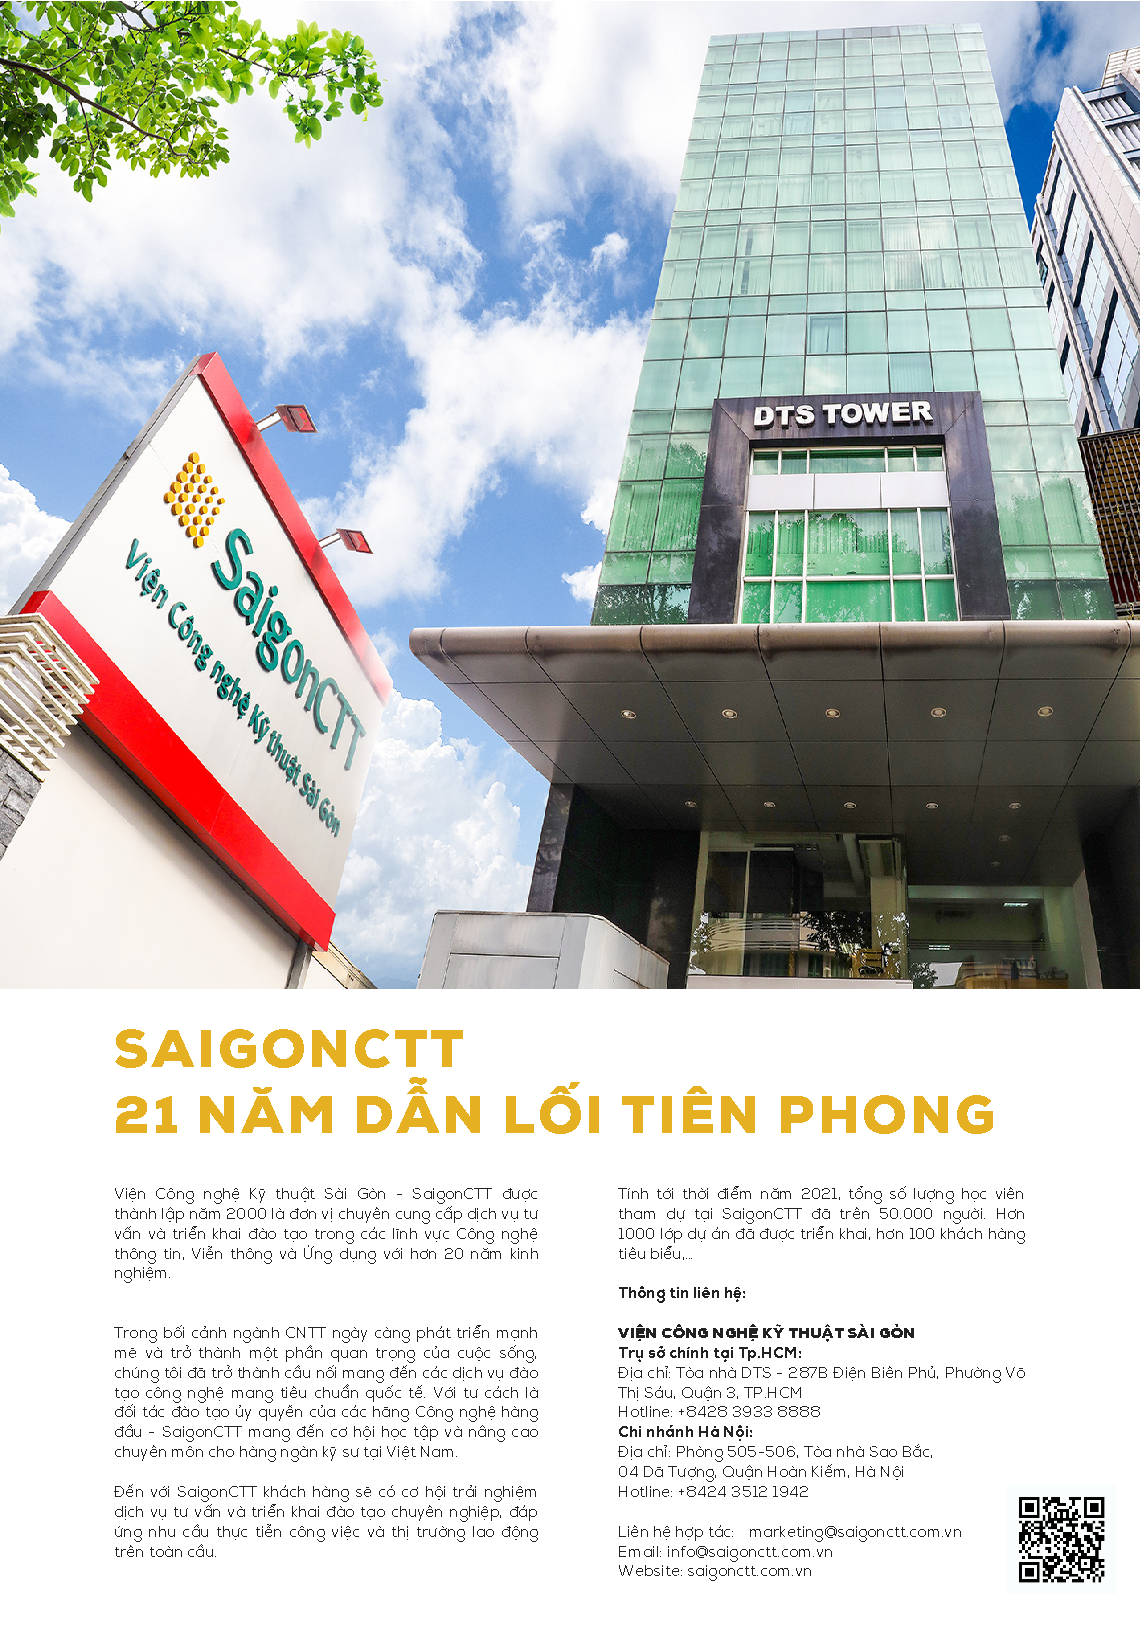
\includegraphics[scale=1]{DTS.pdf}}}
%	\centering
%	\vspace*{0cm}
%	\endgroup
%	\newpage	
%	\pagestyle{empty}
%	
	\setcounter{figure}{0}
	\thispagestyle{toancuabinone}
\pagestyle{toancuabi}
\everymath{\color{toancuabi}}
%\blfootnote{$^1$\color{toancuabi}Đại học Thăng Long.}
\graphicspath{{../toancuabi/pic/}}
\begingroup
\AddToShipoutPicture*{\put(0,616){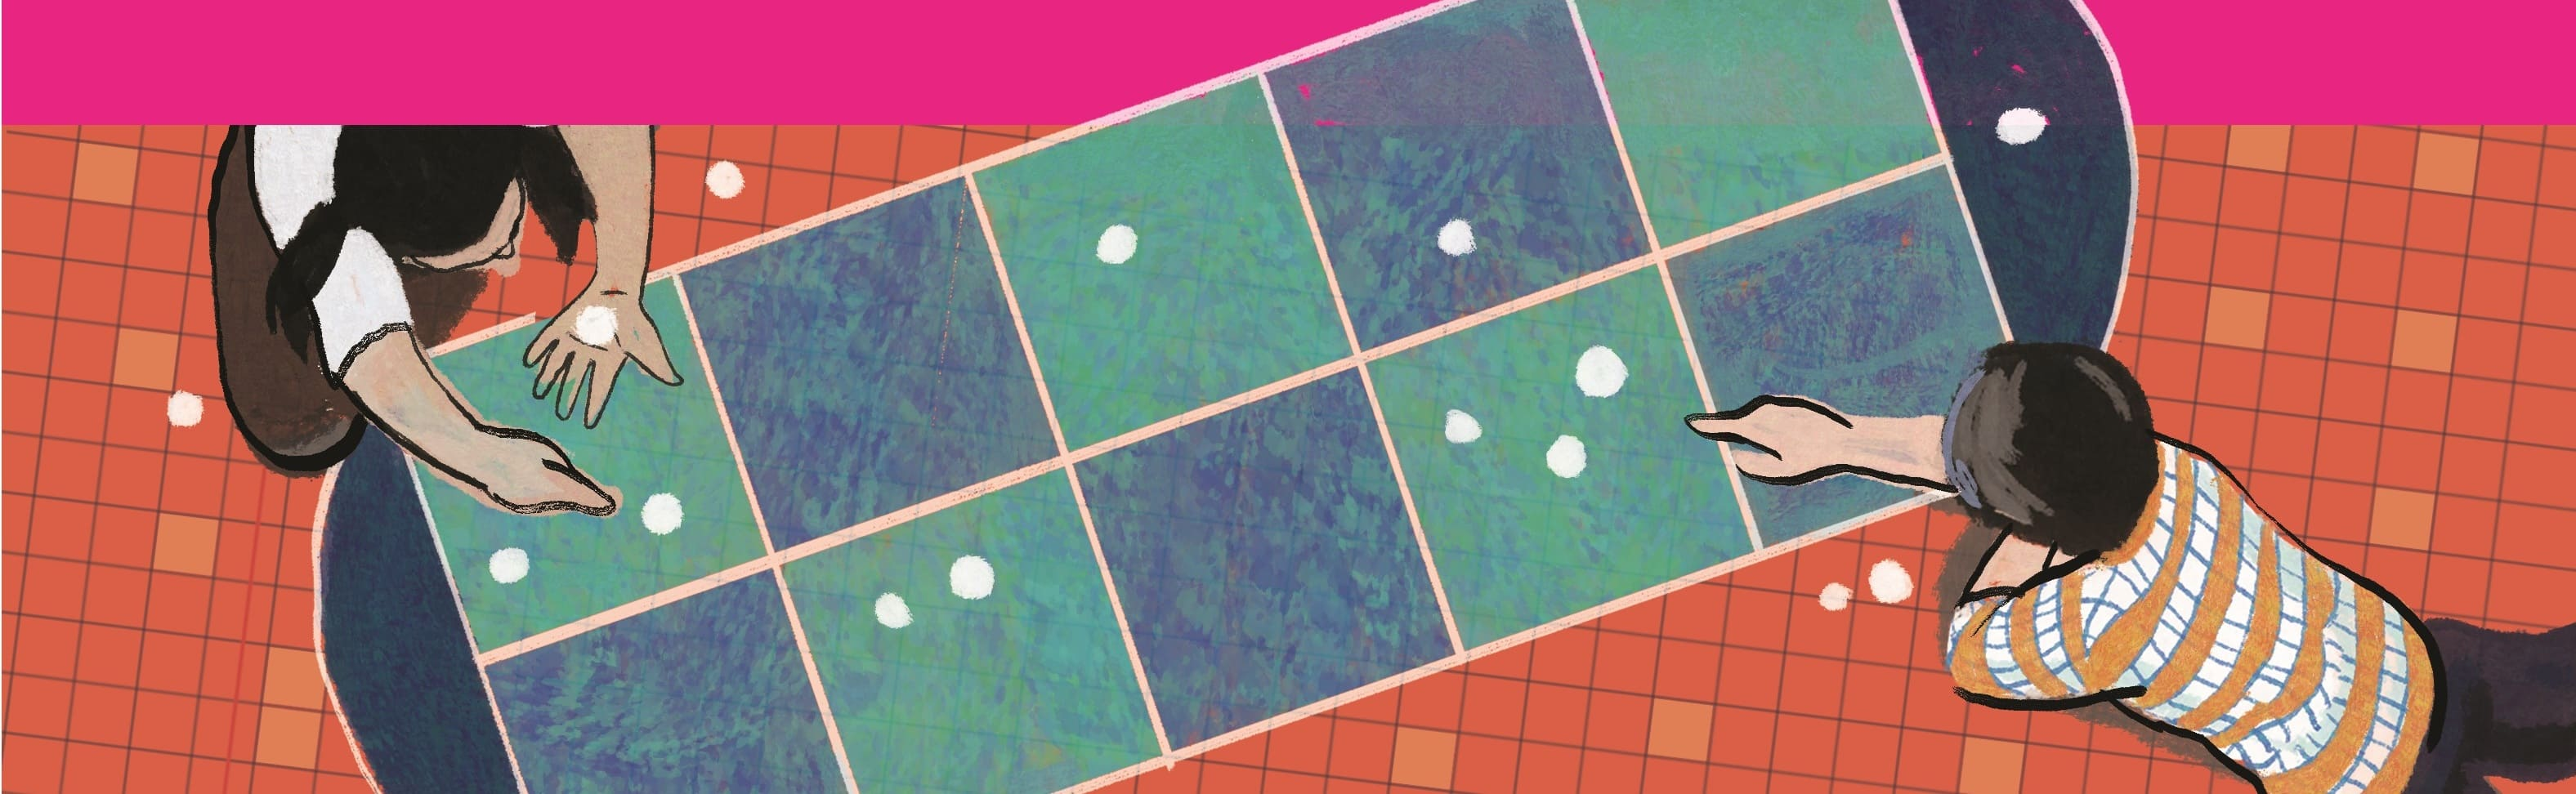
\includegraphics[width=19.3cm]{../bannertoancuabi}}}  
\AddToShipoutPicture*{\put(99,520){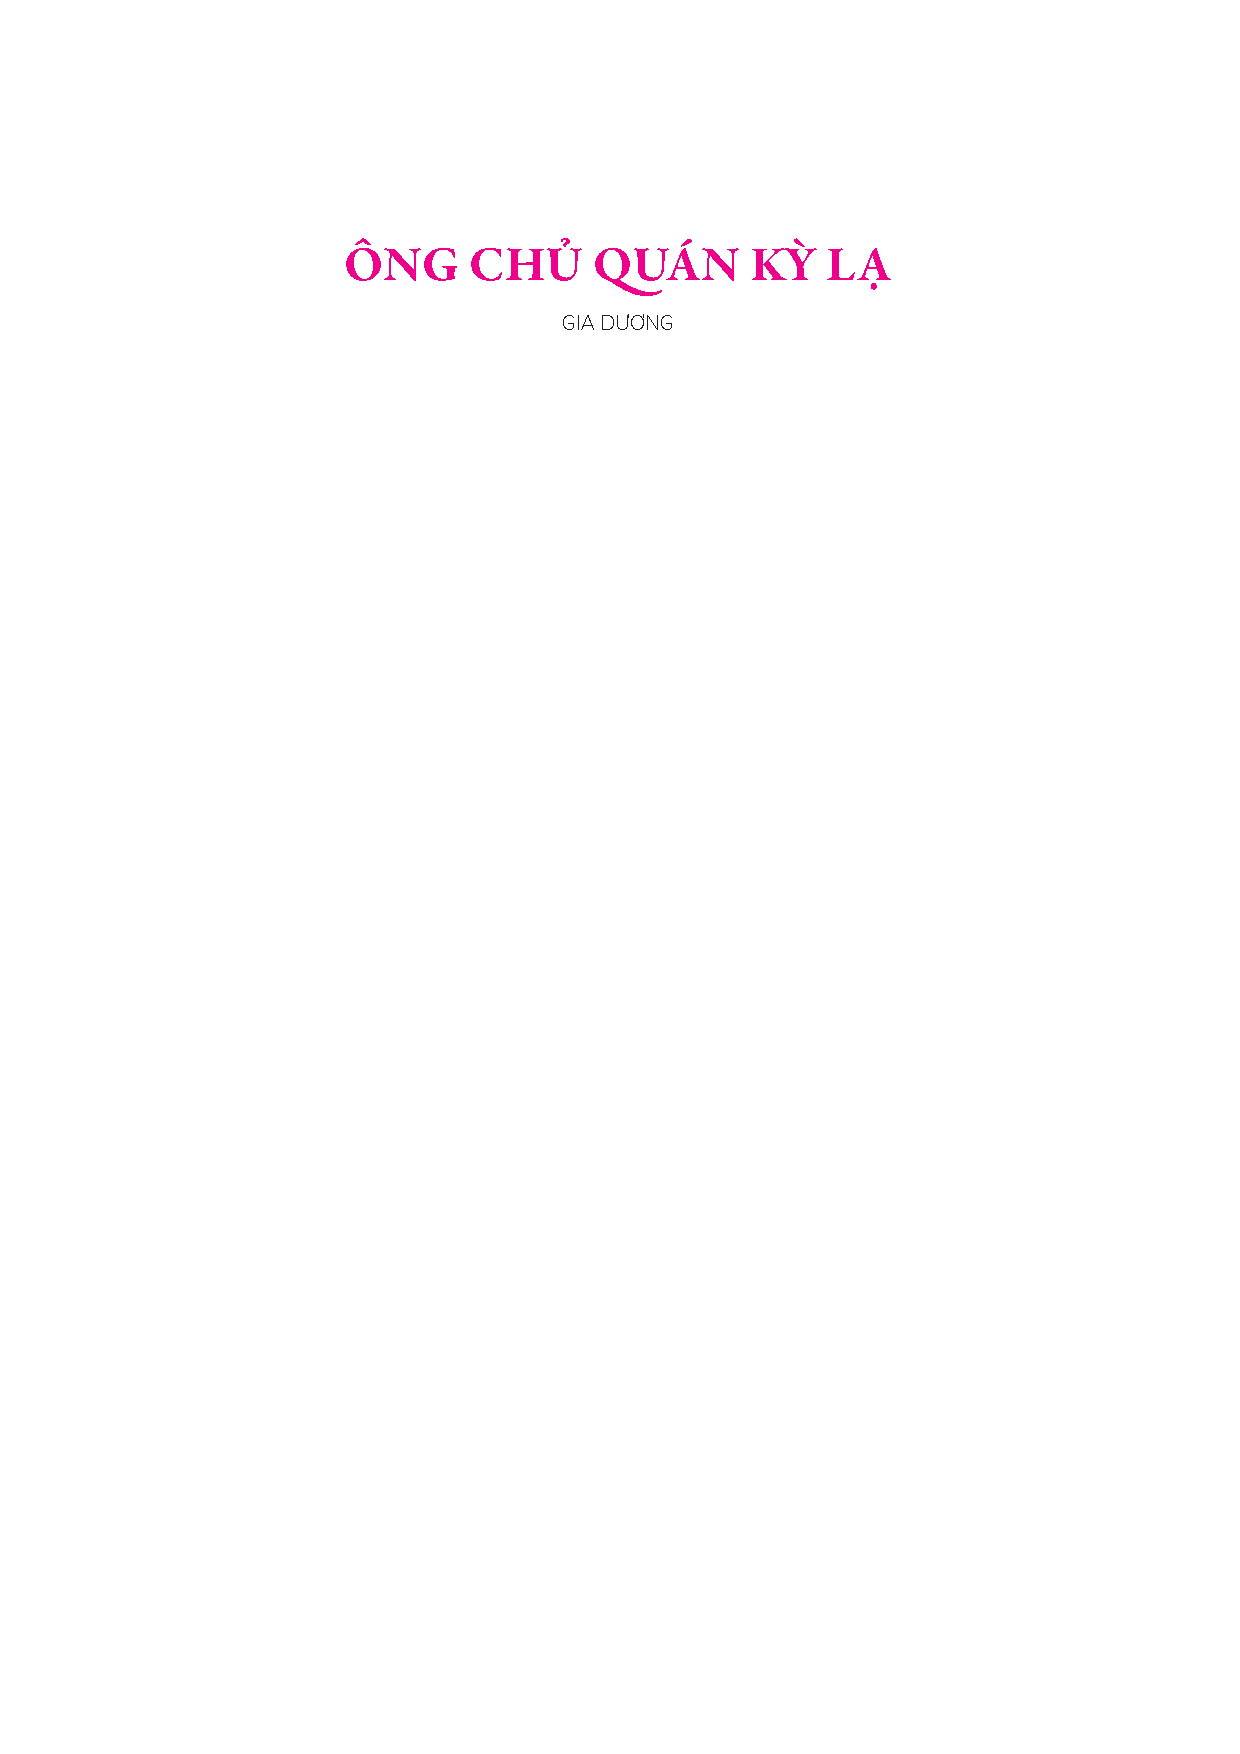
\includegraphics[scale=1]{../tieude.pdf}}} 
\centering
\endgroup
\vspace*{182pt}

%\begin{multicols}{2}
%	Tính diện tích của một hình là một chủ đề hay và có nhiều điều thú vị của các bạn nhỏ cuối cấp $1$. Chủ đề này cũng được các thầy cô trong Câu lạc bộ Unicorn Math Circle (UMC) giảng dạy trong nhiều buổi với sự tham gia hào hứng của các bạn học và có nhiều cách giải độc đáo đã được đưa ra. Chúng ta cùng bắt đầu với một dạng tính diện tích trong những bài giảng của các thầy cô -- Tính diện tích hình trên lưới ô vuông. Với cách tính được trình bày trong bài viết này, các bạn nhỏ chưa cần học đến những công thức tính diện tích vẫn có thể làm được nhé, vì chúng ta chỉ dựa vào các ô vuông trên lưới thôi.
%	\vskip 0.1cm
%	Như nhiều bạn đã biết, lưới ô vuông gồm các đường thẳng song song cách đều nhau theo cả chiều ngang cũng như chiều dọc và tạo thành những hình vuông mà ta quy ước là chiếm $1$ đơn vị diện tích. Dựa vào diện tích của hình vuông đơn vị này chúng ta có thể tính được diện tích của nhiều kiểu hình tạo trên lưới ô vuông.
%	\begin{figure}[H]
%		\centering
%		\vspace*{-5pt}
%		\captionsetup{labelformat= empty, justification=centering}
%		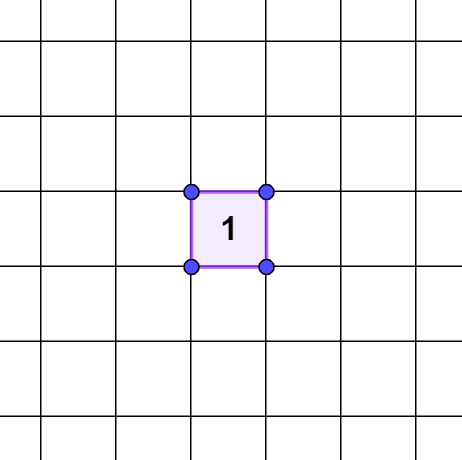
\includegraphics[width=0.48\linewidth]{1}
%%		\caption{\small\textit{\color{}.}}
%		\vspace*{-2pt}
%	\end{figure}
%	Trước hết ta bắt đầu với việc tìm diện tích của những hình rất đơn giản nhưng đóng vai trò quan trọng trong việc tính toán diện tích các hình ở các ví dụ sau.
%	\vskip 0.1cm
%	Hình cơ bản đầu tiên cần tính diện tích là hình chữ nhật có các cạnh nằm trên các đường thẳng của lưới.
%	\vskip 0.1cm
%	\textbf{\color{toancuabi}Ví dụ} $\pmb{1.}$ Tính diện tích hình chữ nhật được tô đậm trong lưới ô vuông dưới đây.  
%	\begin{figure}[H]
%		\centering
%		\vspace*{-5pt}
%		\captionsetup{labelformat= empty, justification=centering}
%		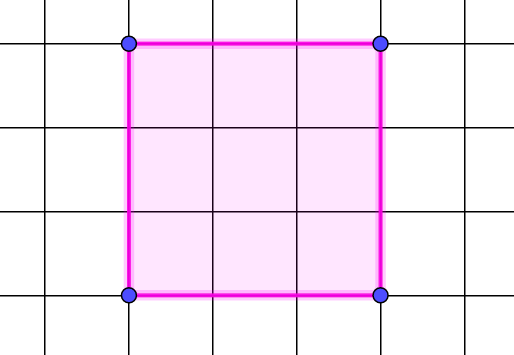
\includegraphics[width=0.55\linewidth]{2}
%		%		\caption{\small\textit{\color{}.}}
%		\vspace*{-10pt}
%	\end{figure}
%	\textit{Lời giải.} Bằng cách đếm trực tiếp, ta thấy rằng có tổng cộng $12$ ô vuông được tô đậm, cho nên diện tích phần hình bằng $12$ đơn vị diện tích.
%	\vskip 0.1cm
%	Các bạn mà học công thức tính diện tích hình chữ nhật rồi sẽ thấy ngay, chiều dài và chiều rộng của hình chữ nhật tương ứng là $4$ và $3$ đơn vị độ dài, từ đó hình chữ nhật có diện tích là: $4 \times 3 = 12$ (đơn vị diện tích).
%	\vskip 0.1cm
%	Chúng ta tiếp tục với hình cơ bản thứ hai là tam giác có hai cạnh trùng với hai đường dọc và ngang của lưới ô vuông.
%	\vskip 0.1cm
%	\textbf{\color{toancuabi}Ví dụ} $\pmb{2.}$ Tính diện tích tam giác được tô đậm trong hình dưới đây.
%	\begin{figure}[H]
%		\centering
%		\vspace*{-5pt}
%		\captionsetup{labelformat= empty, justification=centering}
%		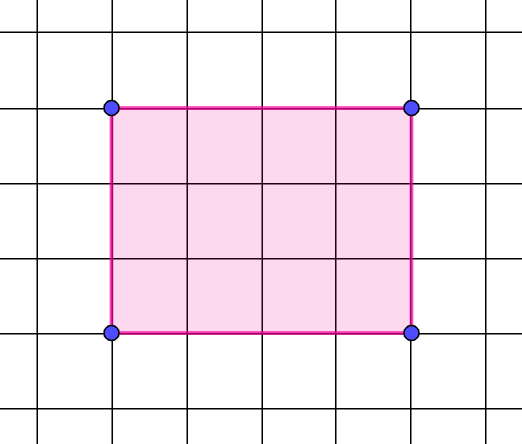
\includegraphics[width=0.55\linewidth]{3}
%		%		\caption{\small\textit{\color{}.}}
%		\vspace*{-10pt}
%	\end{figure}
%	\textit{Lời giải.} Ở ví dụ này, các bạn nhỏ quan sát một chút thì sẽ thấy ngay diện tích của tam giác đã cho bằng một nửa hình chữ nhật màu cỡ $6\times4$ được tô màu xanh dương dưới đây.
%	\begin{figure}[H]
%		\centering
%		\vspace*{-5pt}
%		\captionsetup{labelformat= empty, justification=centering}
%		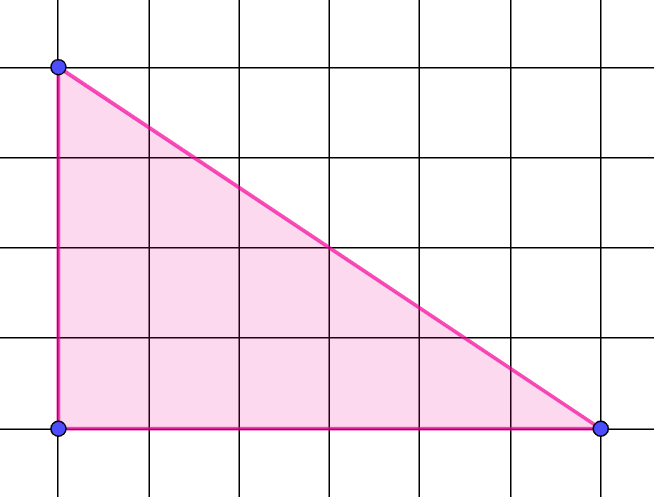
\includegraphics[width=0.55\linewidth]{4}
%		%		\caption{\small\textit{\color{}.}}
%		\vspace*{-10pt}
%	\end{figure}
%	Do diện tích hình chữ nhật được tạo bởi $24$ ô vuông nên diện tích hình tam giác bằng $\dfrac{24}{2} =12$ (đơn vị diện tích).
%	\vskip 0.1cm
%	Ngoài ra, nếu bạn nhỏ nào đã biết công thức tính diện tích tam giác thì tam giác trong Ví dụ $2$ là tam giác vuông với $2$ cạnh góc vuông là $6$ và $4$ đơn vị. Do đó diện tích của tam giác là $d\frac{1}{2}\times 6\times 4 = 12$ đơn vị.
%	\vskip 0.1cm
%	Hai ví dụ trên cho ta một cái nhìn trực quan về bài toán tính diện tích trên lưới ô vuông, ta chỉ dùng cách đếm đơn thuần số ô vuông trên lưới. Trong các bài toán sau, có thể có nhiều cách giải khác nhau nhưng bài viết đưa ra cách giải mà chỉ dựa vào hai hình cơ bản đã biết cách tính diện tích trong Ví dụ $1$ và Ví dụ $2$.
%	\vskip 0.1cm
%	Chúng ta lại tiếp tục với tính diện tích của tam giác nhé. Lần này là tam giác chỉ có một cạnh trùng với đường dọc--ngang của lưới và trong trường hợp này, ta không thể áp dụng luôn cách tính như trong Ví dụ $2$. Tuy nhiên bằng cách chia tam giác này thành các tam giác nhỏ có hai cạnh trùng với những đường thẳng của lưới, ta hoàn toàn có thể áp dụng cách tính diện tích tam giác như trong tình huống trên.
%	\vskip 0.1cm
%	\textbf{\color{toancuabi}Ví dụ} $\pmb{3.}$ Tính diện tích tam giác được tô đậm trong hình cho ở dưới đây.
%	\begin{figure}[H]
%		\centering
%		\vspace*{-5pt}
%		\captionsetup{labelformat= empty, justification=centering}
%		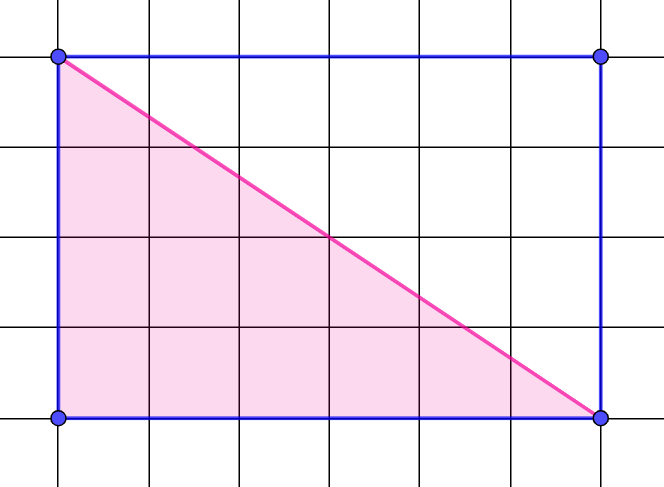
\includegraphics[width=0.55\linewidth]{5}
%		%		\caption{\small\textit{\color{}.}}
%		\vspace*{-10pt}
%	\end{figure}
%	\textit{Lời giải.} Ta chia hình tam giác lớn thành hai hình tam giác $(1)$ và $(2)$.
%	\begin{figure}[H]
%		\centering
%		\vspace*{-5pt}
%		\captionsetup{labelformat= empty, justification=centering}
%		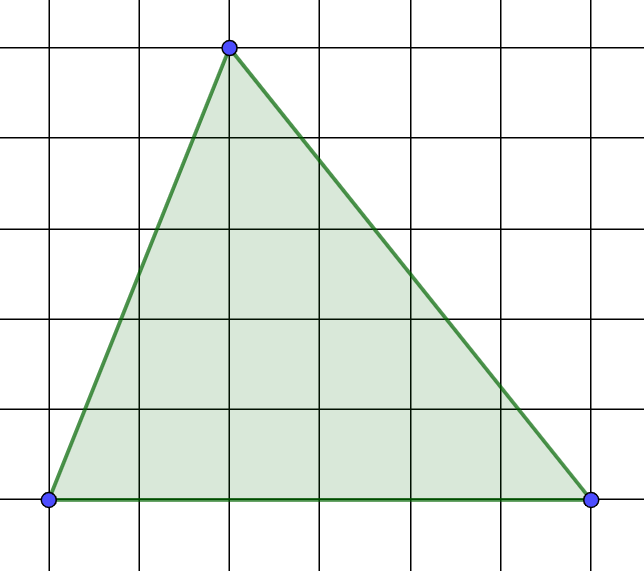
\includegraphics[width=0.55\linewidth]{6}
%		%		\caption{\small\textit{\color{}.}}
%		\vspace*{-10pt}
%	\end{figure}
%	Sau đó tính diện tích từng tam giác, tương tự như trong Ví dụ $2$.
%	\begin{figure}[H]
%		\centering
%		\vspace*{-5pt}
%		\captionsetup{labelformat= empty, justification=centering}
%		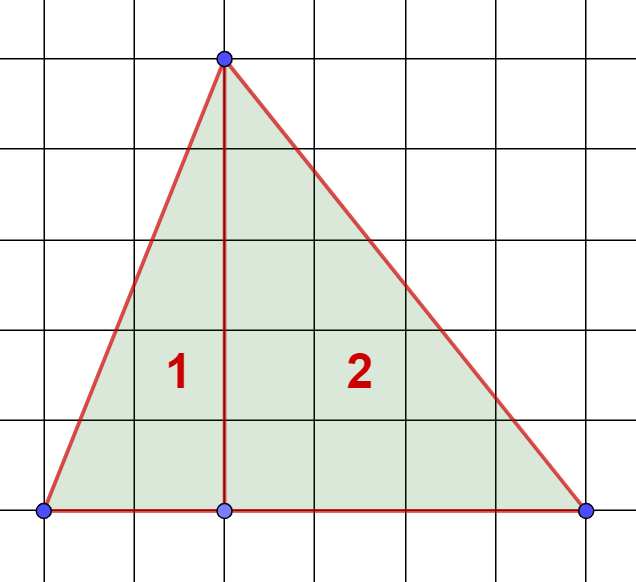
\includegraphics[width=0.55\linewidth]{7}
%		%		\caption{\small\textit{\color{}.}}
%		\vspace*{-10pt}
%	\end{figure}
%	Hình tam giác $(1)$ có diện tích bằng một nửa hình chữ nhật bên trái nên có diện tích là: $\dfrac{10}{2}=5$ (đơn vị diện tích).
%	\vskip 0.1cm
%	Hình tam giác $(2)$ có diện tích bằng một nửa hình chữ nhật bên phải và do đó có diện tích là: $\dfrac{20}{2}=10$ (đơn vị diện tích).
%	\vskip 0.1cm
%	Suy ra hình cần tính có diện tích bằng $5+10=15$ (đơn vị diện tích). 
%	\vskip 0.1cm
%	Tính diện tích bằng cách chia hình thành những hình nhỏ hơn không chỉ dừng lại ở việc tính toán những dạng hình học quen thuộc như hình tam giác, hình chữ nhật, ... mà còn có thể áp dụng cho một hình đặc biệt nào đó. Chẳng hạn như hình ``chú mèo" ngộ nghĩnh dưới đây. 
%	\vskip 0.1cm 
%	\textbf{\color{toancuabi}Ví dụ} $\pmb{4.}$ Tính diện tích ``chú mèo" được cho bởi phần tô đậm trong hình sau.
%	\begin{figure}[H]
%		\centering
%		\vspace*{-5pt}
%		\captionsetup{labelformat= empty, justification=centering}
%		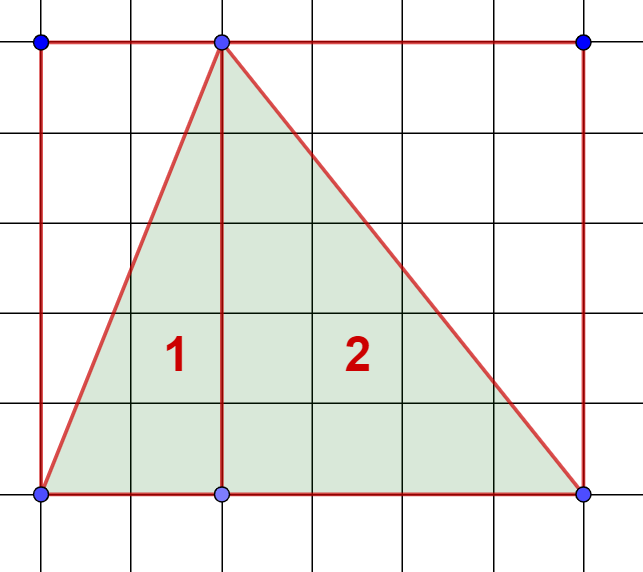
\includegraphics[width=0.5\linewidth]{8}
%		%		\caption{\small\textit{\color{}.}}
%		\vspace*{-10pt}
%	\end{figure}
%	\textit{Lời giải.} Ở hình trên có những tam giác nửa, tức là tam giác có diện tích bằng một nửa hình vuông đơn vị và có diện tích là $\dfrac{1}{2}$ đơn vị diện tích. Ta đếm có tổng cộng $8$ hình vuông và $6$ hình tam giác nửa ($2$ tai, $2$ chân và cái đuôi). Vì thế ``chú mèo" có diện tích bằng $8+\dfrac{1}{2}\times6=11$ đơn vị diện tích.
%	\vskip 0.1cm
%	\textbf{\color{toancuabi}Bài tập} $\pmb{1.}$ Các bạn nhỏ hãy tính diện tích ``chú ngựa" trong hình sau.
%	\begin{figure}[H]
%		\centering
%		\vspace*{-5pt}
%		\captionsetup{labelformat= empty, justification=centering}
%		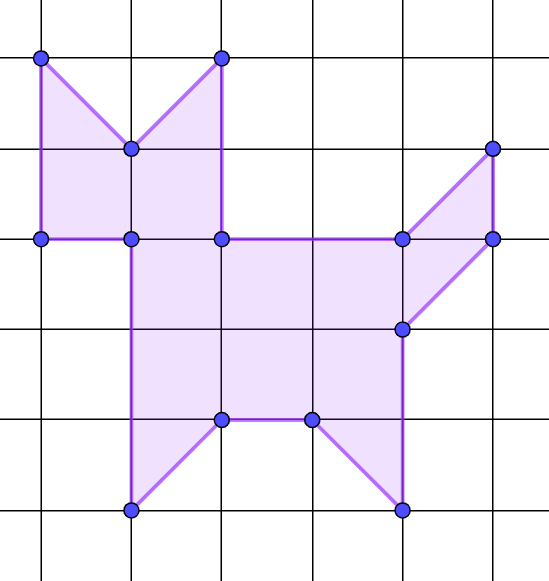
\includegraphics[width=0.58\linewidth]{9}
%		%		\caption{\small\textit{\color{}.}}
%		\vspace*{-10pt}
%	\end{figure}
%	Nếu gặp những tình huống hình mà cần tìm diện tích không thể tính trực tiếp bằng việc đếm số ô vuông, hay không thể chia thành những hình cơ bản đã biết cách tính diện tích; chúng ta có thể xem xét cách tìm thông qua phần bù của nó đối với một hình bao quanh. Để đơn giản, phần bù của hình đã cho thường được lấy trong một hình cơ bản đã biết diện tích như hình chữ nhật có các cạnh trùng với những đường thẳng của lưới. Dưới đây là một số ví dụ về những hình chữ nhật thế này.
%	\begin{figure}[H]
%		\centering
%		\vspace*{5pt}
%		\captionsetup{labelformat= empty, justification=centering}
%		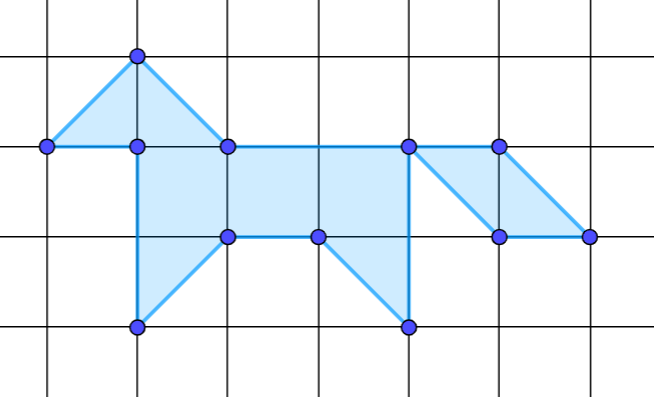
\includegraphics[width=1\linewidth]{10}
%		%		\caption{\small\textit{\color{}.}}
%		\vspace*{-15pt}
%	\end{figure}
%	Diện tích cần tính dưới đây tiếp tục là một tam giác, nhưng lần này là một tam giác tùy ý, không có cạnh nào trùng với những đường thẳng của lưới. 
%	\vskip 0.1cm
%	\textbf{\color{toancuabi}Ví dụ} $\pmb{5.}$ Tính diện tích của hình được tô đậm sau đây.
%	\begin{figure}[H]
%		\centering
%		\vspace*{-5pt}
%		\captionsetup{labelformat= empty, justification=centering}
%		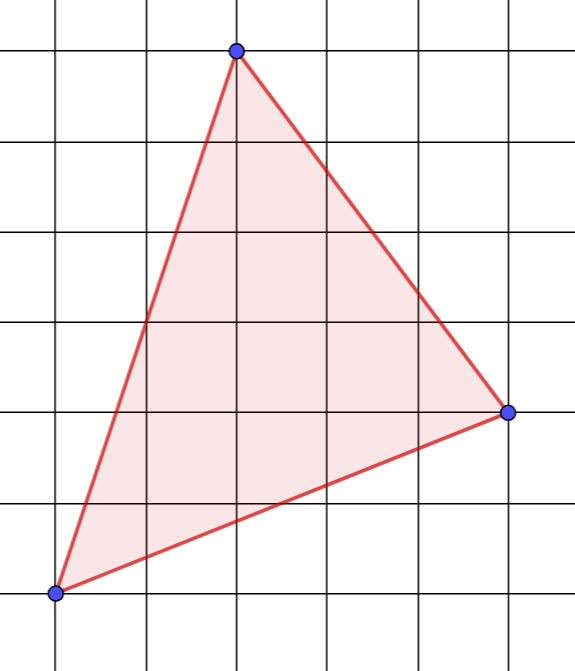
\includegraphics[width=0.5\linewidth]{11}
%		%		\caption{\small\textit{\color{}.}}
%		\vspace*{-10pt}
%	\end{figure}
%	\textit{Lời giải.} Rõ ràng với tam giác này, việc tính trực tiếp phần bên trong là khó khăn. Tuy nhiên phần bù của tam giác trong hình chữ nhật bao quanh nó lại là những tam giác như trong Ví dụ $2$ nên ta hoàn toàn có thể tính được ngay.
%	\begin{figure}[H]
%		\centering
%		\vspace*{-5pt}
%		\captionsetup{labelformat= empty, justification=centering}
%		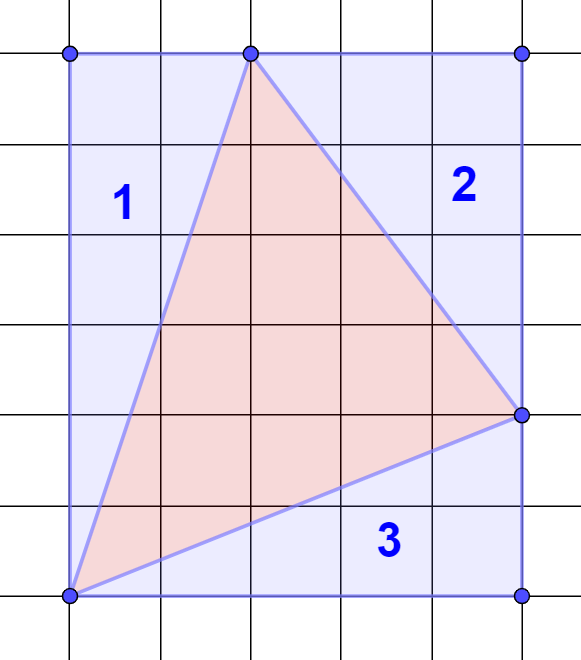
\includegraphics[width=0.5\linewidth]{12}
%		%		\caption{\small\textit{\color{}.}}
%		\vspace*{-10pt}
%	\end{figure}
%	Lần lượt gọi ba tam giác phần bù được tô xanh là $(1)$,$(2)$ và $(3)$. Ta thấy
%	Hình $(1)$ có diện tích bằng nửa hình chữ nhật cỡ $6\times2$, nên có diện tích bằng $6$.
%	\vskip 0.1cm
%	Hình $(2)$ có diện tích bằng nửa hình chữ nhật cỡ $4\times3$, nên có diện tích bằng $6$.
%	\vskip 0.1cm
%	Hình $(3)$ có diện tích bằng nửa hình chữ nhật cỡ $5\times2$, nên có diện tích bằng $5$.
%	\vskip 0.1cm
%	Vì phần bù được tạo thành bởi ba tam giác vuông $(1)$, $(2)$ và $(3)$ nên diện tích của chúng bằng $6+6+5=17$. Suy ra diện tích tam giác được tô đậm bằng $30-17=13$ đơn vị diện tích.
%	\vskip 0.1cm
%	Để rèn luyện thêm cách tính diện tích dựa trên phần bù, chúng ta cùng luyện tập tiếp những ví dụ sau nhé. 
%	\vskip 0.1cm 
%	\textbf{\color{toancuabi}Ví dụ} $\pmb{6.}$ Tính diện tích phần hình được tô đậm dưới đây.
%	\begin{figure}[H]
%		\centering
%		\vspace*{-5pt}
%		\captionsetup{labelformat= empty, justification=centering}
%		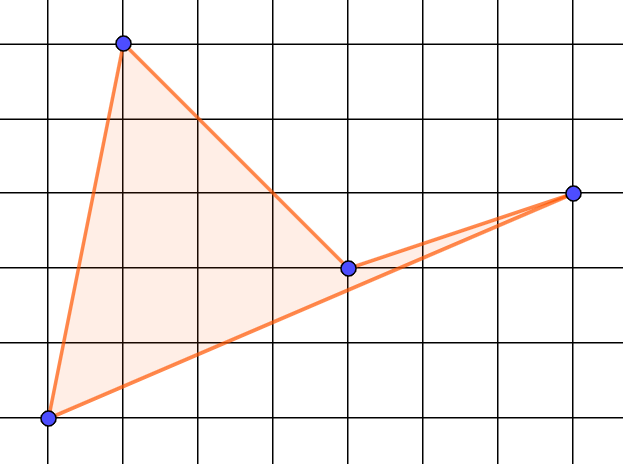
\includegraphics[width=0.6\linewidth]{13}
%		%		\caption{\small\textit{\color{}.}}
%		\vspace*{-10pt}
%	\end{figure}
%	\textit{Lời giải.} Trong ví dụ này, ta tiếp tục tính diện tích theo phần bù và chia phần bù của hình đã cho thành các hình quen thuộc đã biết cách tính diện tích. Mỗi bạn nhỏ có thể chọn những cách chia khác nhau, chẳng hạn ta có thể chia đơn giản như sau: 
%	\begin{figure}[H]
%		\centering
%		\vspace*{-5pt}
%		\captionsetup{labelformat= empty, justification=centering}
%		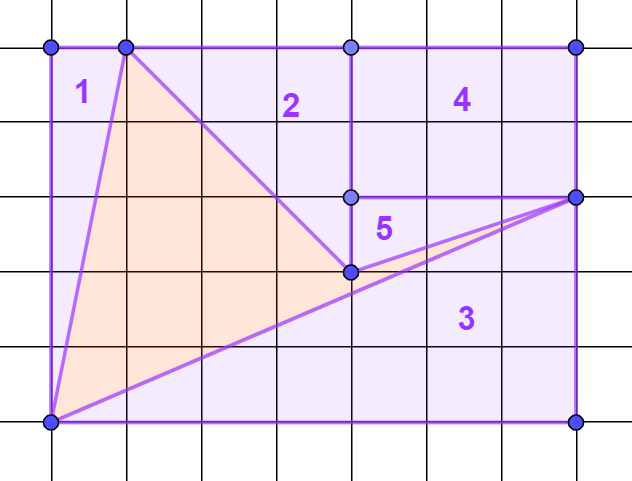
\includegraphics[width=0.6\linewidth]{14}
%		%		\caption{\small\textit{\color{}.}}
%		\vspace*{-10pt}
%	\end{figure}
%	Phần bù của hình đã cho được chia thành năm hình $(1)$, $(2)$, $(3)$, $(4)$ và $(5)$. Khi đó
%	\vskip 0.1cm
%	Hình tam giác $(1)$ có diện tích bằng $\dfrac{1}{2} \times 5=2{,}5$ (đơn vị diện tích)
%	\vskip 0.1cm
%	Hình tam giác $(2)$ có diện tích bằng $\dfrac{1}{2} \times9 =4{,}5$ (đơn vị diện tích)
%	\vskip 0.1cm
%	Hình tam giác $(3)$ có diện tích bằng $\dfrac{1}{2} \times 21=10{,}5$ (đơn vị diện tích)
%	\vskip 0.1cm
%	Hình chữ nhật $(4)$ có diện tích bằng $6$ (đơn vị diện tích)
%	\vskip 0.1cm
%	Hình tam giác $(5)$ có diện tích bằng $\dfrac{1}{2} \times3=1{,}5$ (đơn vị diện tích)
%	\vskip 0.1cm
%	Vậy tổng diện tích của chúng bằng $2{,}5+4{,}5+10{,}5+6+1{,}5 =25$. Suy ra diện tích hình tam giác tô đậm bằng $7\times 7-25=24$ đơn vị diện tích. 
%	\vskip 0.1cm
%	Qua những ví dụ trên, các bạn nhỏ chắc là đã biết các tính qua phần bù rồi đúng không? Bài tập sau để chúng ta luyện tập thêm nhé. 
%	\vskip 0.1cm
%	\textbf{\color{toancuabi}Bài tập} $\pmb{2.}$ Tính diện tích phần hình được tô đậm trong các hình dưới đây.
%	\begin{figure}[H]
%		\centering
%		\vspace*{-5pt}
%		\captionsetup{labelformat= empty, justification=centering}
%		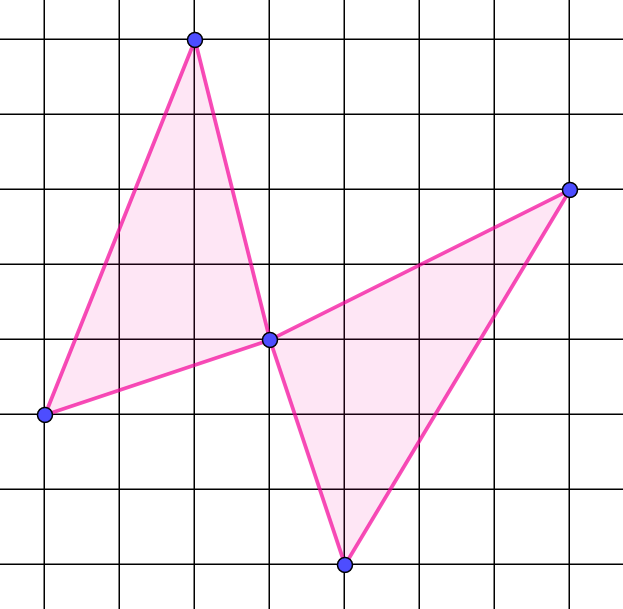
\includegraphics[width=0.55\linewidth]{15}
%		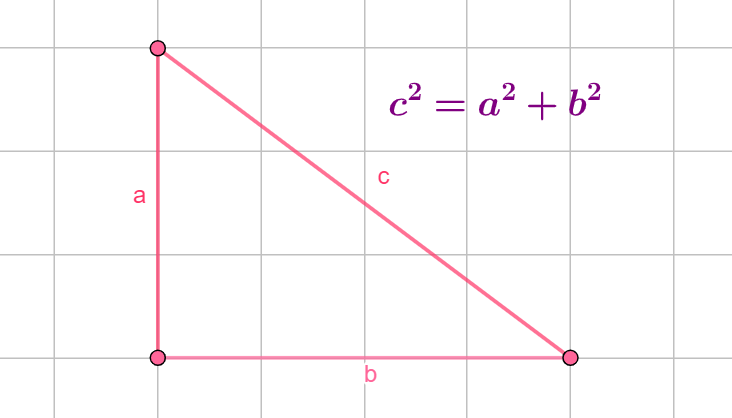
\includegraphics[width=0.48\linewidth]{16}
%		%		\caption{\small\textit{\color{}.}}
%		\vspace*{-10pt}
%	\end{figure}
%	Việc tính theo phần bù chỉ hiệu quả khi phần bù được cấu tạo bởi những hình cơ bản như hình chữ nhật, hình tam giác như trong hai ví dụ đầu tiên. Vì thế các bạn nhỏ cần chia thật khéo, sao cho mọi hình đều có dạng quen thuộc nhé!  
%	\vskip 0.1cm
%	Đôi khi trong quá trình làm bài, có thể các bạn nhỏ sẽ gặp phải tình huống thế này: sau khi đọc xong đề, ta biết chắc rằng bài đó không thể làm theo cách trực tiếp và do đó ta nghĩ tới cách tính theo phần bù. Nhưng mà nếu tính theo phần bù, thậm chí đã có thao tác chia hình, thì cũng chưa chắc tìm ra đáp án ngay được. Lúc này các bạn nhỏ có thể nghĩ tới việc tính những phần bù này bằng cách lấy bù trong một hình khác. Ví dụ sau minh họa diện tích được tính theo cách này.  
%	\vskip 0.1cm
%	\textbf{\color{toancuabi}Ví dụ} $\pmb{7.}$ Tính diện tích phần hình được tô đậm (AFHI) trong hình dưới đây
%	\begin{figure}[H]
%		\centering
%%		\vspace*{-5pt}
%		\captionsetup{labelformat= empty, justification=centering}
%		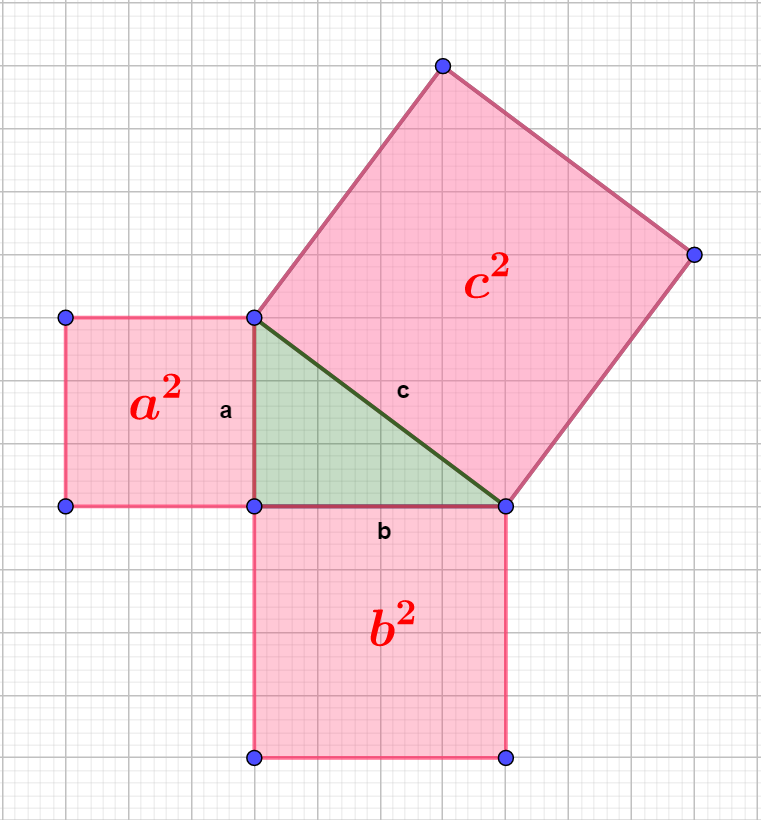
\includegraphics[width=1\linewidth]{17}
%		%		\caption{\small\textit{\color{}.}}
%		\vspace*{-15pt}
%	\end{figure}
%	\textit{Lời giải.} Việc tính toán trực tiếp là không dễ dàng trong trường hợp này, do đó ta thử tính theo cách lấy phần bù nhé. Ta bao hình đã cho bởi đa giác $AJIHFDCB$, là ghép của ba hình vuông $ABCE$, $EDFG$ và $GHIJ$. Khi đó phần bù của đa giác $AFHI$ là tam giác $AIJ$ và đa giác $ABCDF$.
%	\vskip 0.1cm
%	Các bạn nhỏ dễ dàng tính được diện tích tam giác $AIJ$, nhưng với đa giác $ABCDF$ thì tính như thế nào nhỉ? 
%	\vskip 0.1cm
%	Trước hết, ta có ngay diện tích tam giác $AIJ$ bằng một nửa hình chữ nhật cỡ $12\times3$, nên có diện tích là: $\dfrac{1}{2}\times 36=18$ (đơn vị diện tích). 
%	\begin{figure}[H]
%		\centering
%%		\vspace*{-5pt}
%		\captionsetup{labelformat= empty, justification=centering}
%		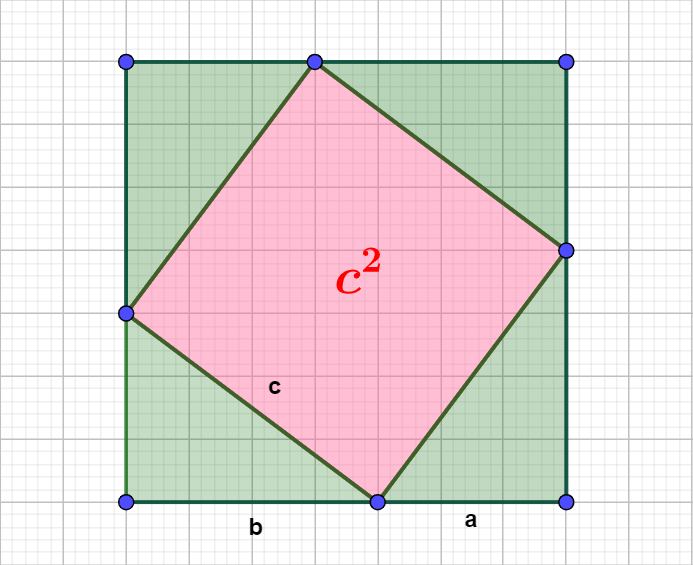
\includegraphics[width=1\linewidth]{18}
%		%		\caption{\small\textit{\color{}.}}
%		\vspace*{-15pt}
%	\end{figure}
%	Tiếp theo là xét tới đa giác $ABCDF$. Mặc dù có thể tính trực tiếp bằng cách chia đa giác thành $3$ tam giác $ABC$, $CDF$ và $ACF$, tuy nhiên việc tìm diện tích tam $ACF$ tương đối dài! Để ý kỹ một chút các bạn nhỏ sẽ thấy rằng nếu lấy đa giác $ABCDF$ ghép với hình chữ nhật $BKDC$ ở góc trên cùng bên trái, thì sẽ thu được tam giác vuông $AKF$ có diện tích bằng một nửa hình chữ nhật cỡ $9\times5$; hay nói cách khác, ta đang đi tính diện tích phần bù theo một phần bù khác. 
%	\vskip 0.1cm
%	Từ hình vẽ ta có nhận xét rằng, 
%	\begin{align*}
%		S_{AKF}=S_{ABCDF}+S_{BKDC},
%	\end{align*} 
%	Suy ra diện tích đa giác $ABCDF$ bằng  $\dfrac{1}{2} \times45-4=18{,}5$ (đơn vị diện tích). 
%	\vskip 0.1cm
%	Như vậy $S_{AFHI}=50-S_{ABCDF}-S_{AIJ}=50-18{,}5-18=13{,}5$ (đơn vị diện tích). 
%	\vskip 0.1cm
%	Ngoài cách làm ở trên ra thì các bạn nhỏ có thể nhìn nhận bài toán theo hướng khác như sau:  đa giác $AFHI$ thực chất nằm trong hình chữ nhật $AKLJ$, khi đó phần bù gồm tam giác $AKF$, hình chữ nhật $FLIH$ và tam giác $AIJ$. 
%	\begin{figure}[H]
%		\centering
%%		\vspace*{-5pt}
%		\captionsetup{labelformat= empty, justification=centering}
%		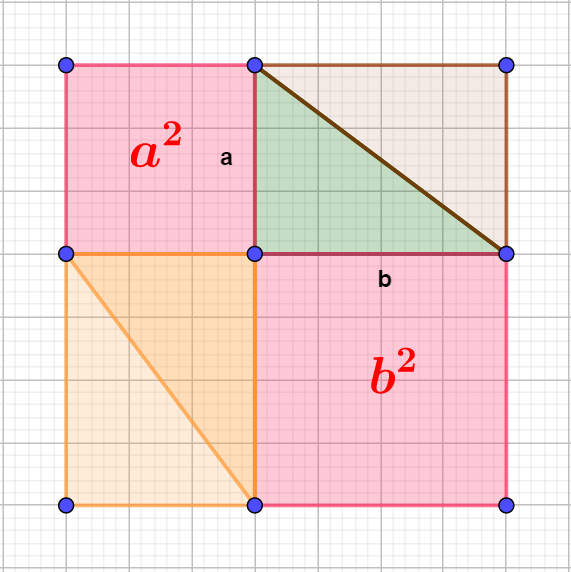
\includegraphics[width=1\linewidth]{19}
%		%		\caption{\small\textit{\color{}.}}
%		\vspace*{-15pt}
%	\end{figure}
%	Vậy diện tích đa giác $AFHI$ bằng 
%	\begin{align*}
%		S_{AFHI}&=S_{AKLJ}-S_{FLIH}-S_{AKF}-S_{AIJ}\\ 
%		&=12\times5-6-22{,}5-18\\
%		&=13{,}5 \text{ (đơn vị diện tích)}.
%	\end{align*}
%	Từ Ví dụ $7$ ta thấy rằng việc tính diện tích bằng phần bù có rất nhiều cách làm khác nhau, chủ yếu phụ thuộc vào cách nhìn hình học của từng bạn.   
%	\vskip 0.1cm
%	Bài tập sau để các em luyện tập thêm nhé.
%	\vskip 0.1cm
%	\textbf{\color{toancuabi}Bài tập} $\pmb{3.}$ Tính diện tích các phần hình được tô đậm dưới đây.
%		\begin{figure}[H]
%		\centering
%		\vspace*{-5pt}
%		\captionsetup{labelformat= empty, justification=centering}
%		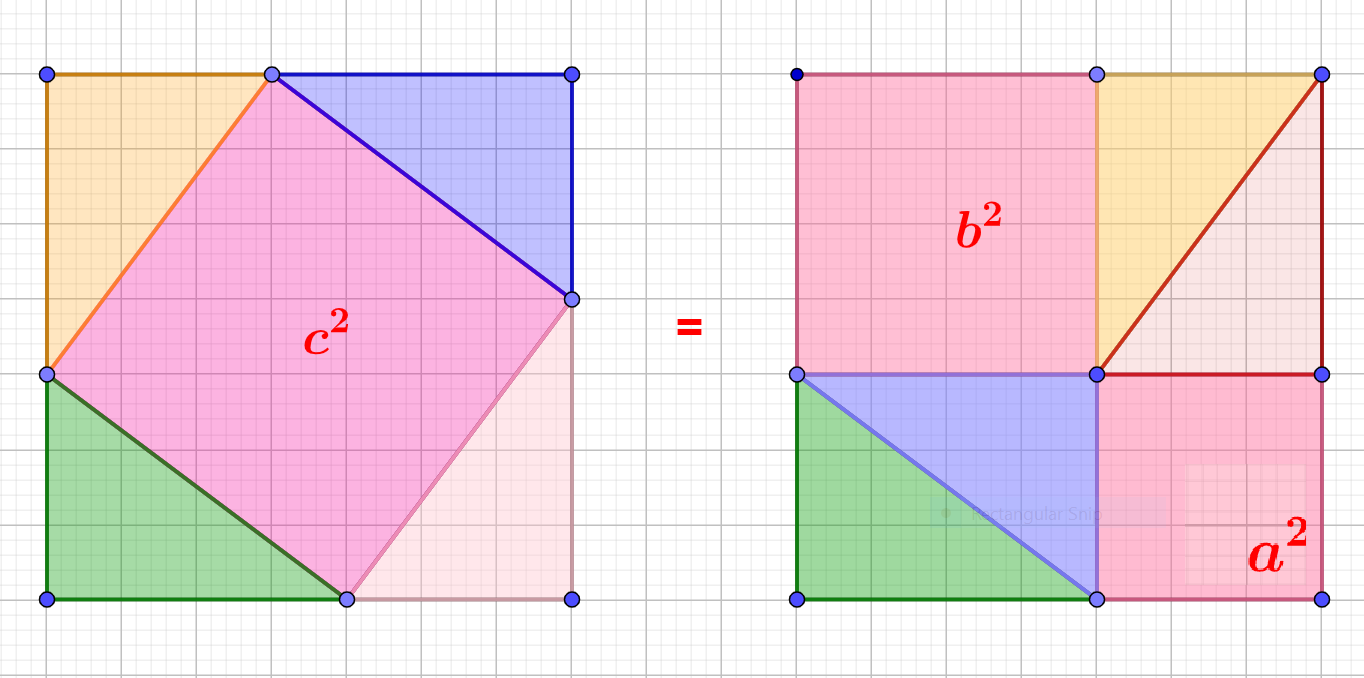
\includegraphics[width=1\linewidth]{20}
%		%		\caption{\small\textit{\color{}.}}
%		\vspace*{-15pt}
%	\end{figure}
%\begin{figure}[H]
%	\centering
%	\vspace*{5pt}
%	\captionsetup{labelformat= empty, justification=centering}
%	\includegraphics[width=0.58\linewidth]{21}
%	%		\caption{\small\textit{\color{}.}}
%	\vspace*{-10pt}
%\end{figure}
%	Vậy là chúng ta đã cùng nhau tìm hiểu về một số phương pháp thường sử dụng khi làm bài toán tính diện tích trên lưới kẻ ô vuông. Tuy rằng tư tưởng của mỗi phương pháp không quá khó hiểu, nhưng các bạn nhỏ vẫn cần luyện tập thường xuyên để có được phản xạ nhanh nhất khi làm bài nhé. Trên thực tế rất nhiều phương pháp độc đáo khác nữa mà bài viết chưa đề cập tới, bạn nhỏ nào hứng thú với dạng bài này có thể tự tìm hiểu thêm, chắc chắn sẽ rất thú vị đấy! Hẹn gặp lại các em trong những chủ đề tiếp theo của câu lạc bộ Unicorn Math Circle.
%\end{multicols}
%\vspace*{-10pt}
%\rule{1\linewidth}{0.1pt}
%\begingroup
%\AddToShipoutPicture*{\put(130,485){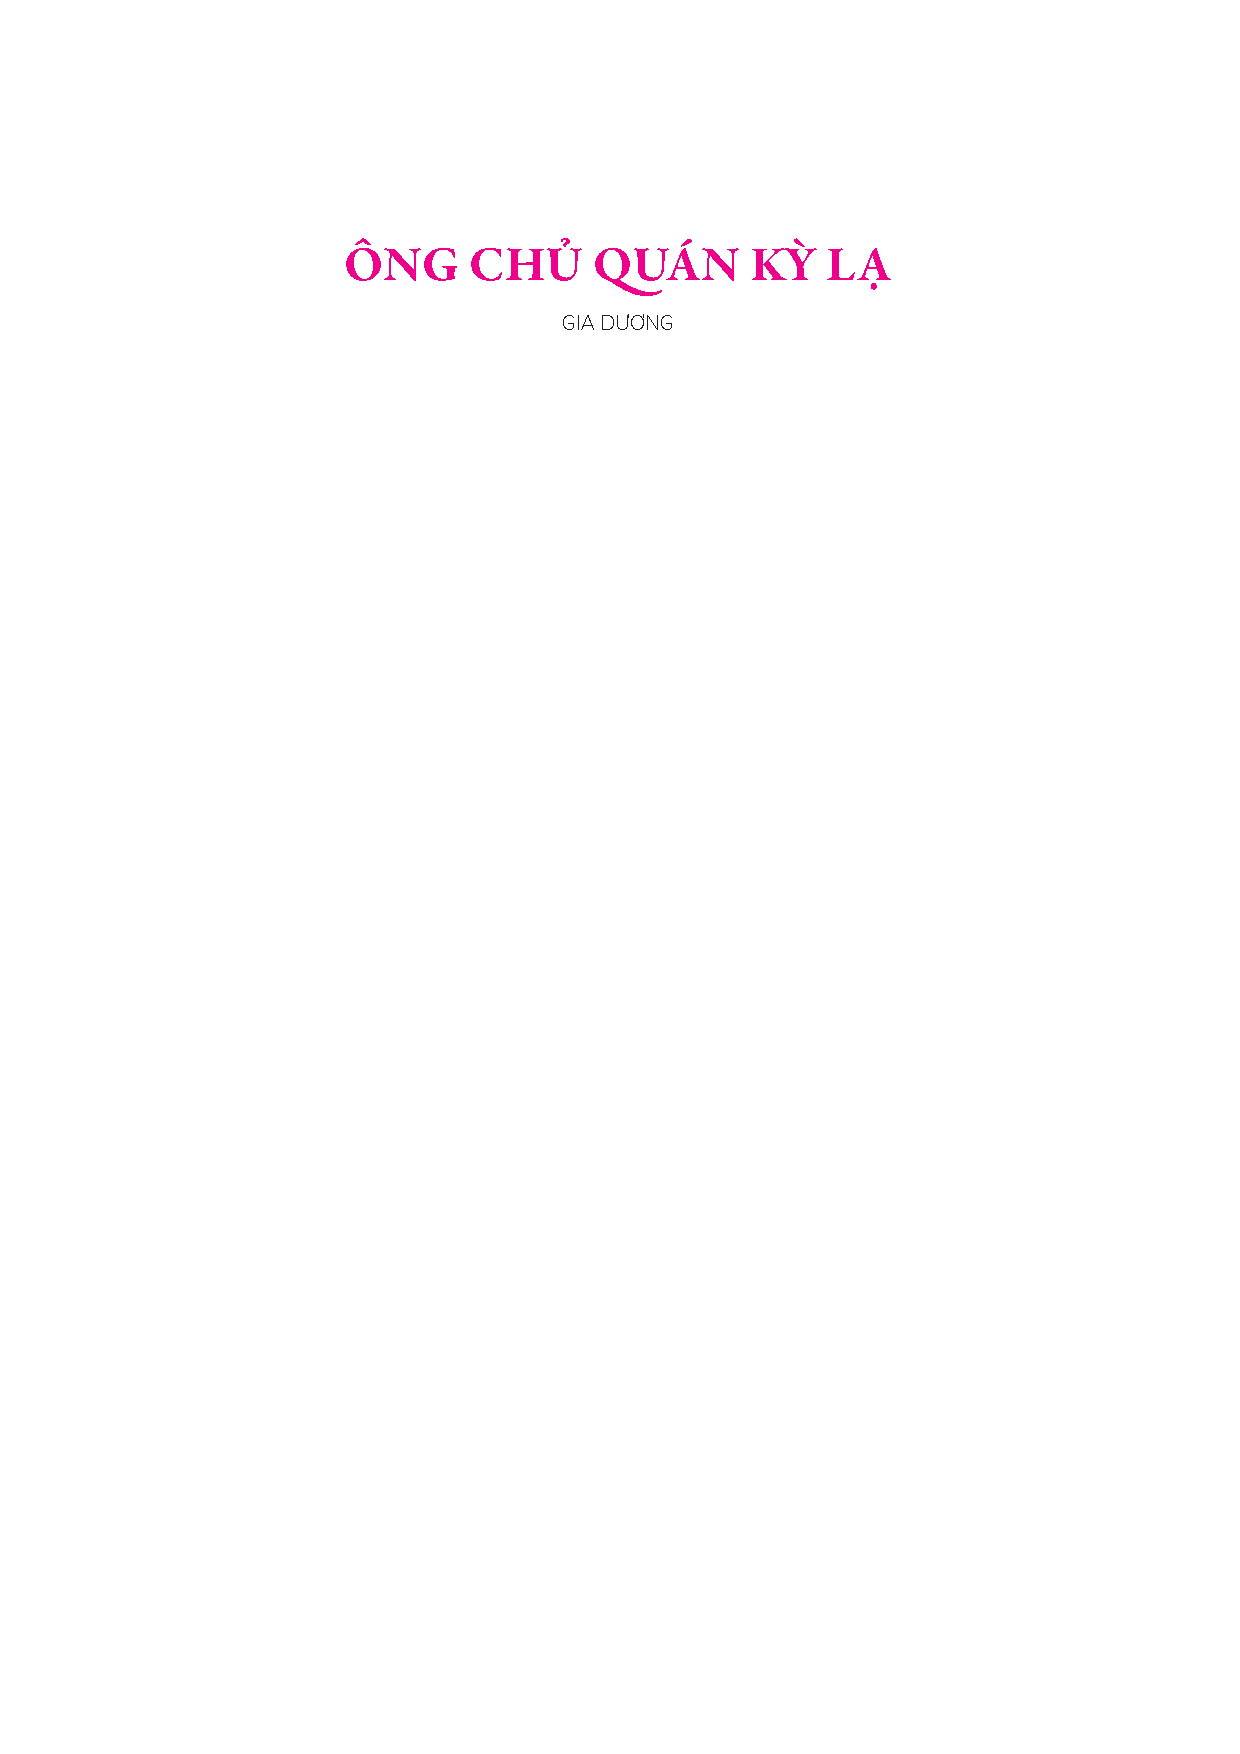
\includegraphics[scale=1]{../tieude.pdf}}} 
%\centering
%\endgroup
%\vspace*{48pt}
\begin{multicols}{2}
	Thám tử Xuân Phong cùng vợ là bà Xuân Bích tham gia một buổi dã ngoại cùng với hai cặp vợ chồng khác. Cả hai ông chồng là các nhà báo nổi tiếng, còn các bà vợ của họ cũng đều là các quý bà danh giá trong thành phố. Kết thúc buổi dã ngoại, cả ba cặp vợ chồng cùng quay trở về nhà và ra tới một con sông và họ phải chèo trên một chiếc thuyền nhỏ để vượt qua sông. Thuyền chỉ có thể chở được một lúc đồng thời hai người, và hơn nữa không có một phụ nữ nào trong họ lại biết chèo thuyền.
	\begin{figure}[H]
		\centering
		\vspace*{-5pt}
		\captionsetup{labelformat= empty, justification=centering}
		\includegraphics[width=1\linewidth]{xuanphong}
		\vspace*{-15pt}
	\end{figure}
	Bỗng dưng, đang lúc hào hứng ôn kể lại các câu chuyện điều tra phá án của mình, thám tử Xuân Phong đâm ra xích mích, giận mặt đỏ tía tai với hai nhà báo kia về phương pháp điều tra đặc biệt thông minh của mình. Thấy tình hình trở nên căng thẳng như vậy, bà Xuân Bích cũng quyết định đứng về phía chồng mình và không thèm nói chuyện với hai quý bà kia cho bõ tức. còn hai quý bà thì ra sức can ngăn hai ông chồng nóng tính của mình và vẫn giữ hoà khí với thám tử Xuân Phong đáng kính.
	\vskip 0.1cm
	Vậy em có thể giúp Xuân Phong và mọi người tìm ra cách để tất cả các thành viên tham gia buổi dã ngoại đều có thể vượt qua sông, sao cho hai người đang giận dỗi nhau thì không ngồi trên thuyền cùng một lúc, và cũng không đứng đồng thời trên cùng một bờ sông. Và một yêu cầu đặc biệt đặt ra nữa là không một nhà báo nào có thể ở lại một mình trên bất kỳ bờ sông nào cùng với hai quý bà mà không có chồng của bà kia. 
	\vskip 0.1cm
	Bài đố này không khó nhưng rất ít, chỉ khoảng $1$ người trong số $1000$ người tham gia giải, mới có thể giải được ra đáp số mà lại không phải dùng đến giấy và bút đấy các em~ạ!
	
\end{multicols}
\newpage
\begingroup
\AddToShipoutPicture*{\put(112,672){
\includegraphics[scale=1]{../tieude11.pdf}}} 
\centering
\endgroup
\vspace*{35pt}

\begin{multicols}{2}
	$\pmb{1.}$ Một chiếc tàu cao tốc dài $18$ m đi ngang qua một cột cây số trong vòng $9$ giây. Hỏi chiếc tàu đó cần bao nhiêu thời gian để đi qua hết một cây cầu dài $36$ m. 
	\begin{figure}[H]
		\centering
		\vspace*{-10pt}
		\captionsetup{labelformat= empty, justification=centering}
		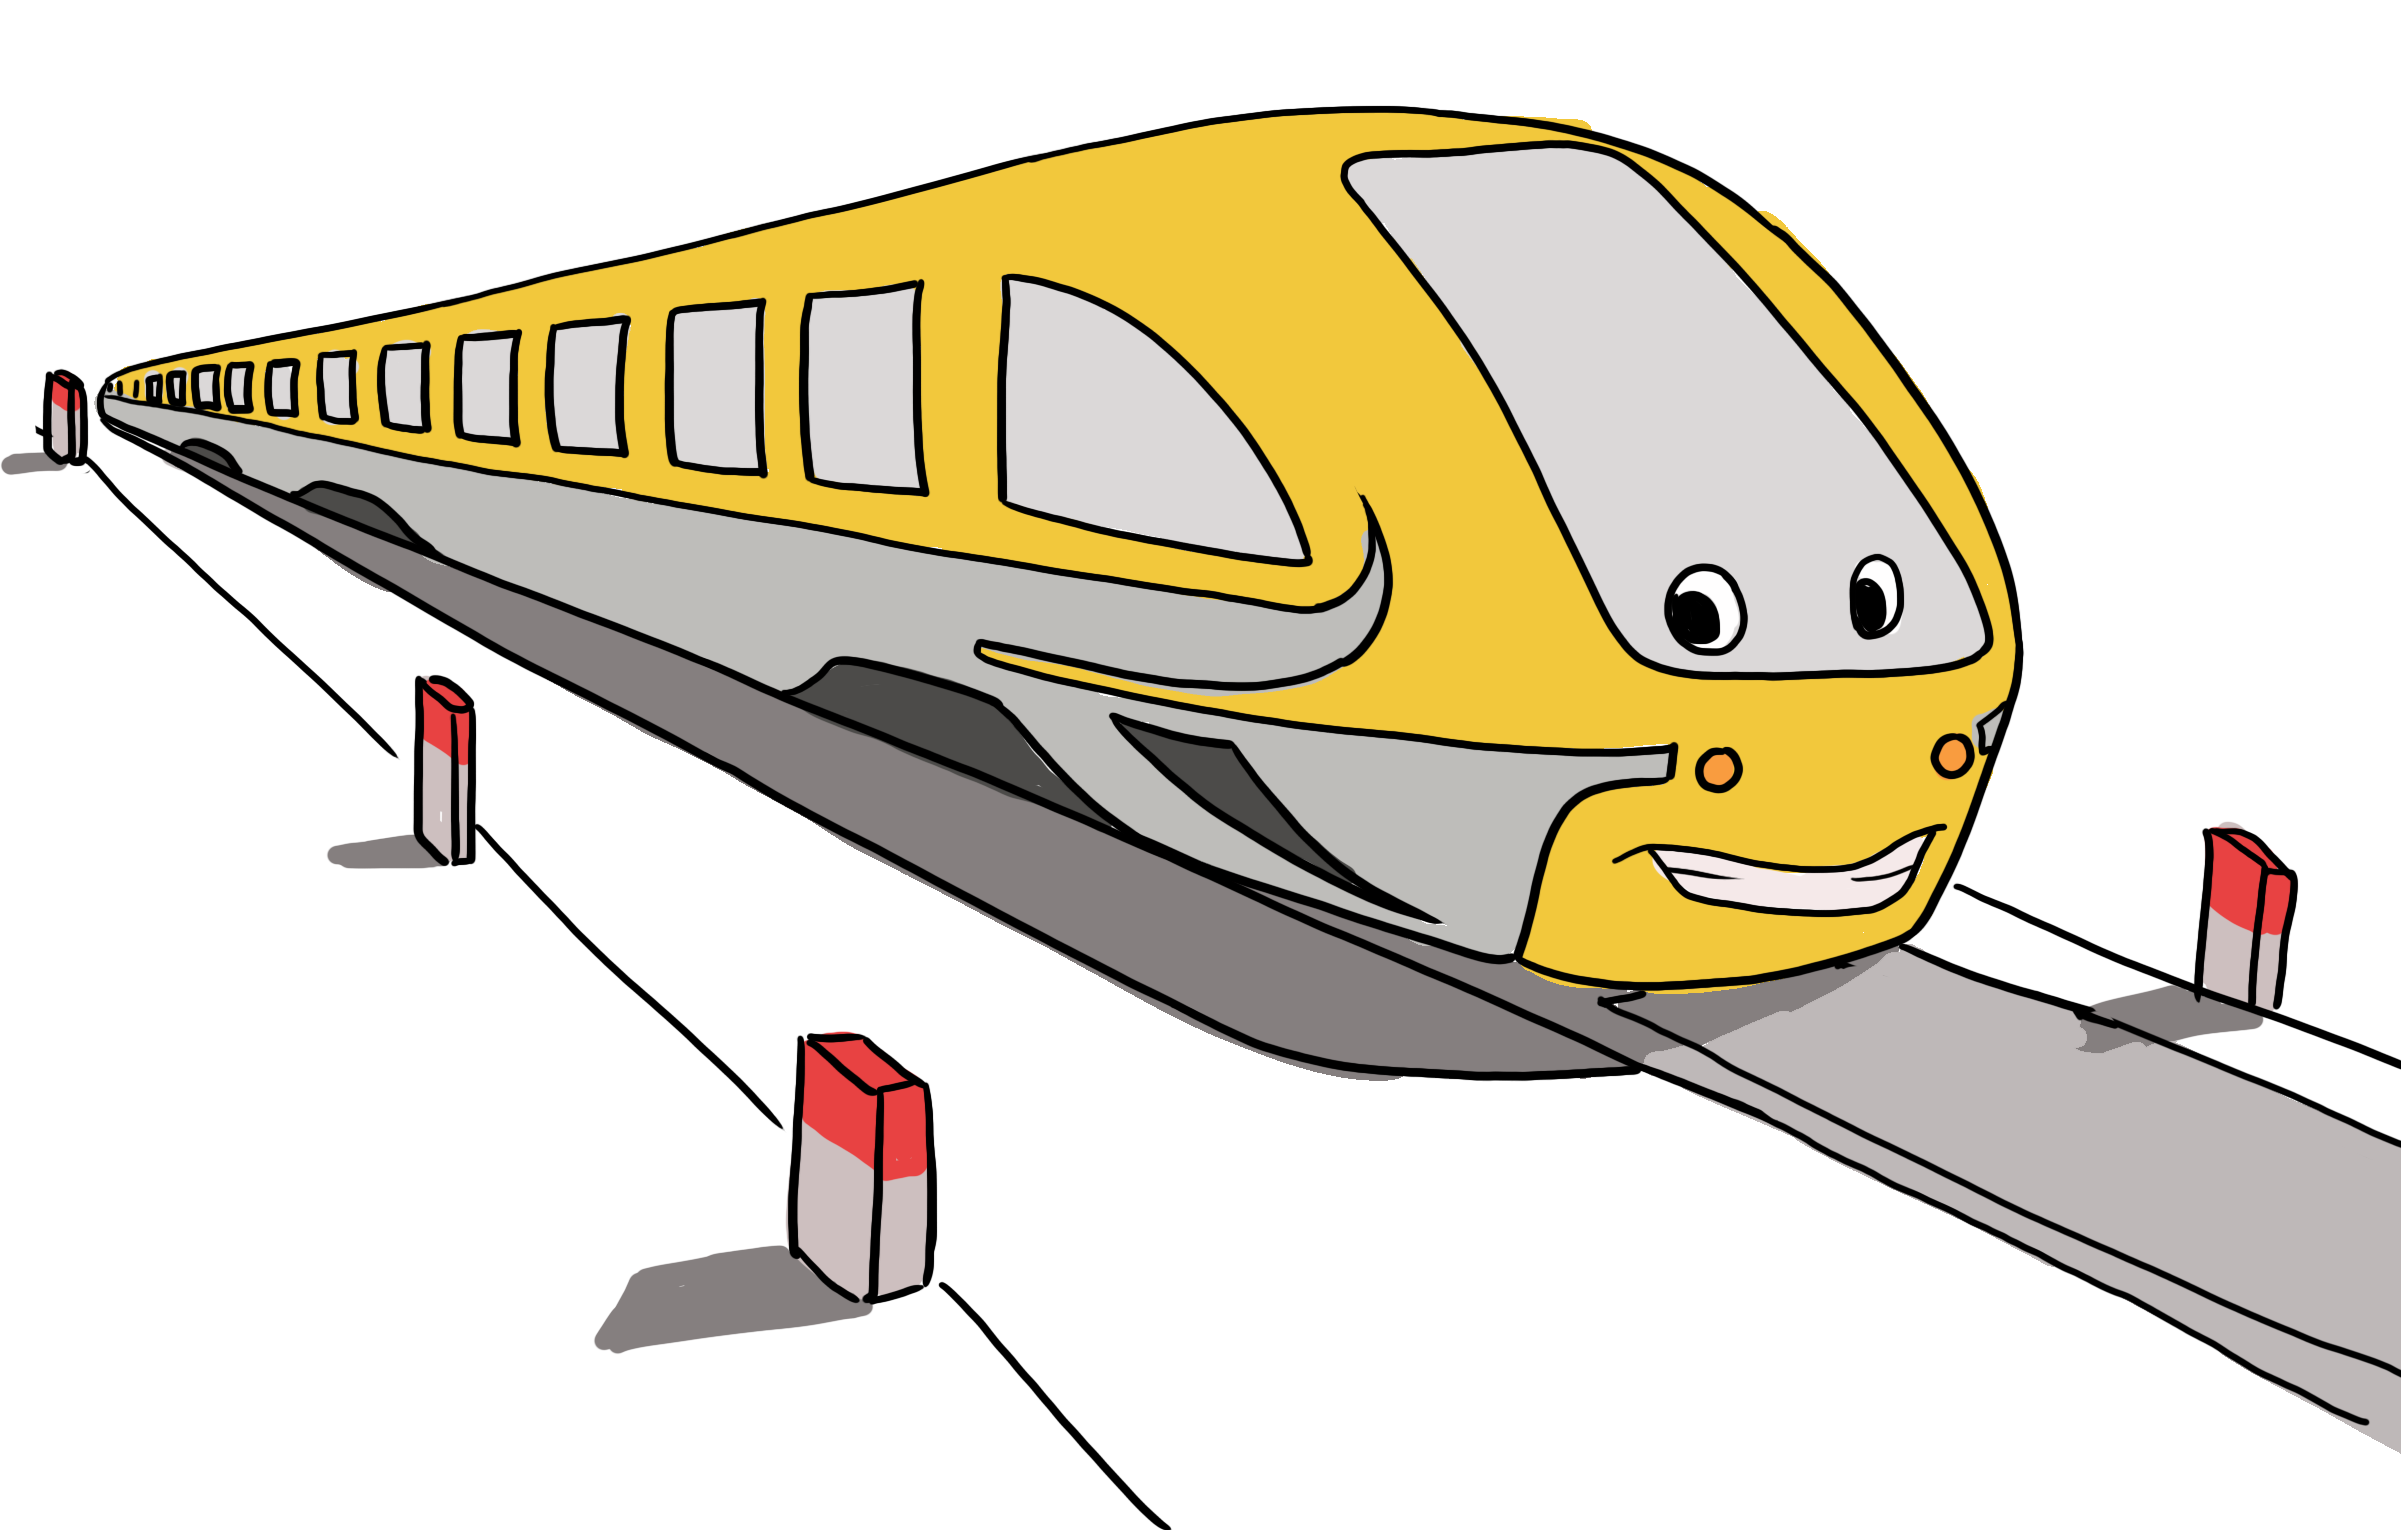
\includegraphics[width=1\linewidth]{Pi10_ToanBi_Bai1}
		\vspace*{-15pt}
	\end{figure}
	\vskip 0.1cm
	$\pmb{2.}$ Hai cậu bé đi bán cam để gây quỹ xây dựng thư viện. Mỗi cậu có $30$ quả cam. Cậu thứ nhất bán  $10{.}000$ đồng hai quả cam, cậu thứ hai bán $10{.}000$ đồng ba quả cam. Trong lúc đang chuẩn bị bày cam ra bán thì một cậu bị gọi về nhà nên cậu ta nhờ cậu thứ hai bán hộ số cam của mình. Tất cả số cam còn lại được cậu bé thứ hai bán với giá $20{.}000$ đồng năm quả. Nếu như số cam bán riêng như dự định lúc đầu thì đã thu được là $150{.}000$ đồng và $100{.}000$ đồng, tức là tổng cộng có $250{.}000$ đồng, nhưng vì bán gộp $20{.}000$ đồng cho $5$ quả nên  hai cậu chỉ thu được $240{.}000$ đồng. Hỏi số tiền bị hụt $10{.}000$ đồng đã mất ở chỗ nào?
	\begin{figure}[H]
		\centering
		\vspace*{-10pt}
		\captionsetup{labelformat= empty, justification=centering}
		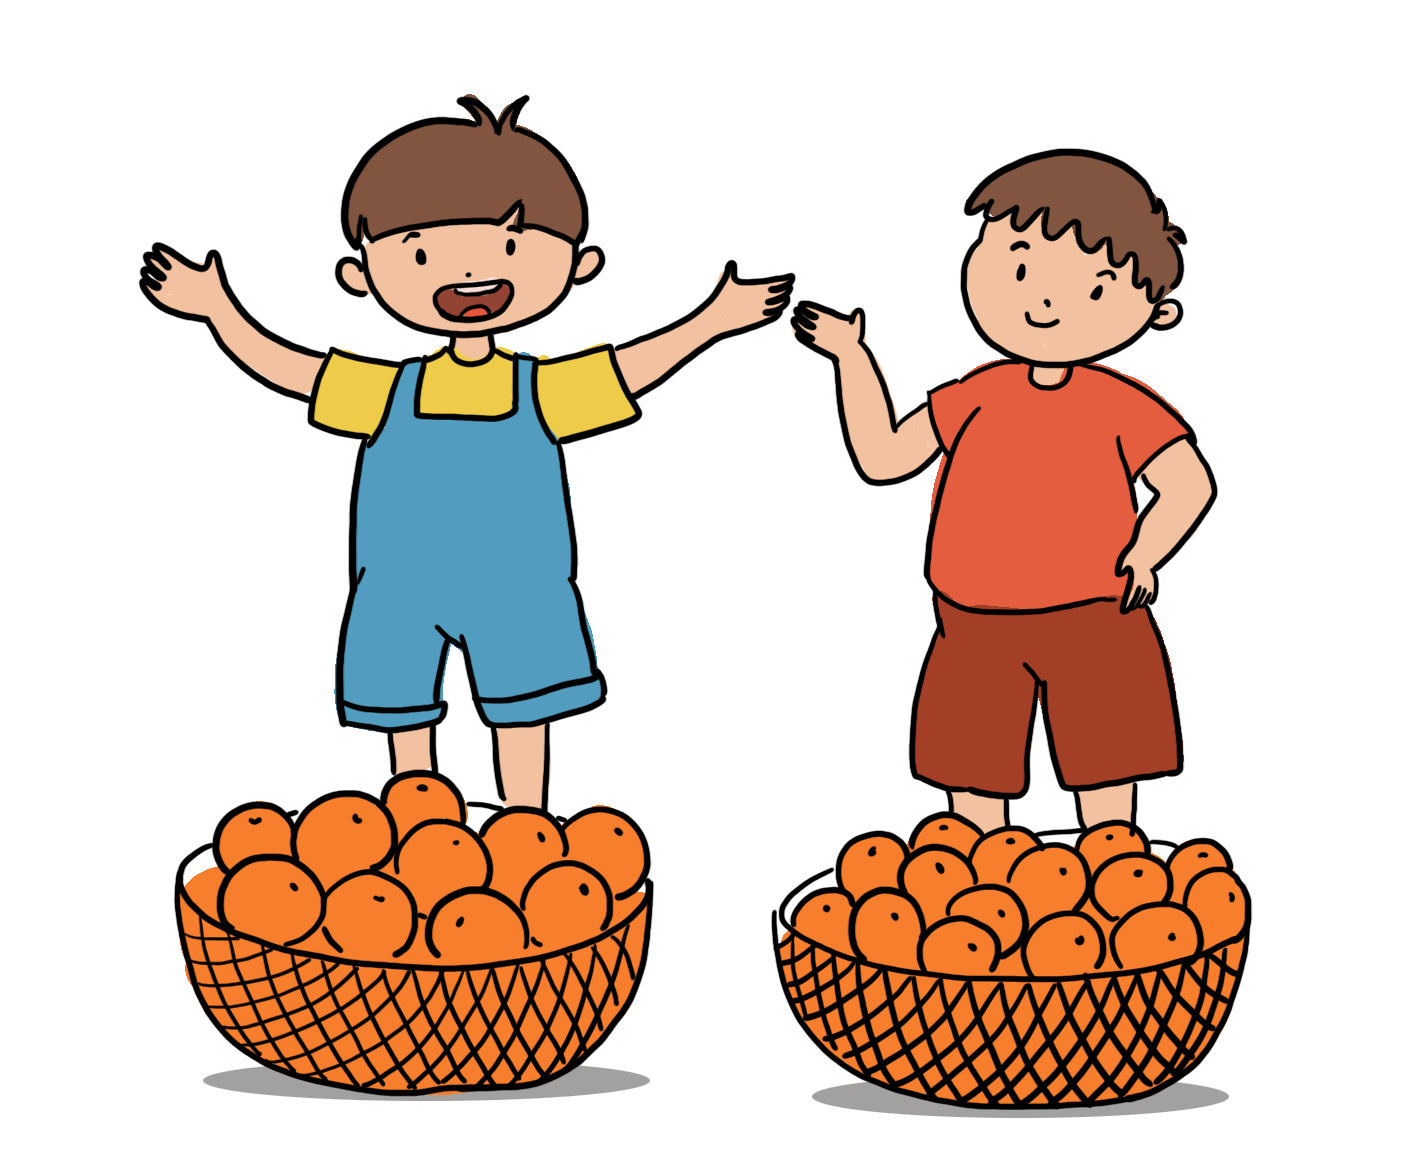
\includegraphics[width=0.8\linewidth]{Pi10_ToanBi_Bai2}
		\vspace*{-10pt}
	\end{figure}
	\vskip 0.1cm
	$\pmb{3.}$ Có ba người bạn tập trung lại để đi cắm trại và họ chỉ có duy nhất một chiếc xe máy có $2$ chỗ ngồi. Liệu họ có thể vượt được quãng đường dài $60$ km tới nơi cắm trại sau khoảng thời gian $3$ giờ đồng hồ được hay không, biết rằng vận tốc của mỗi người đi bộ là $5$ km/giờ và vận tốc của xe máy (có tải hay không có tải) luôn là $50$ km/giờ?
	\begin{figure}[H]
		\centering
		\vspace*{-5pt}
		\captionsetup{labelformat= empty, justification=centering}
		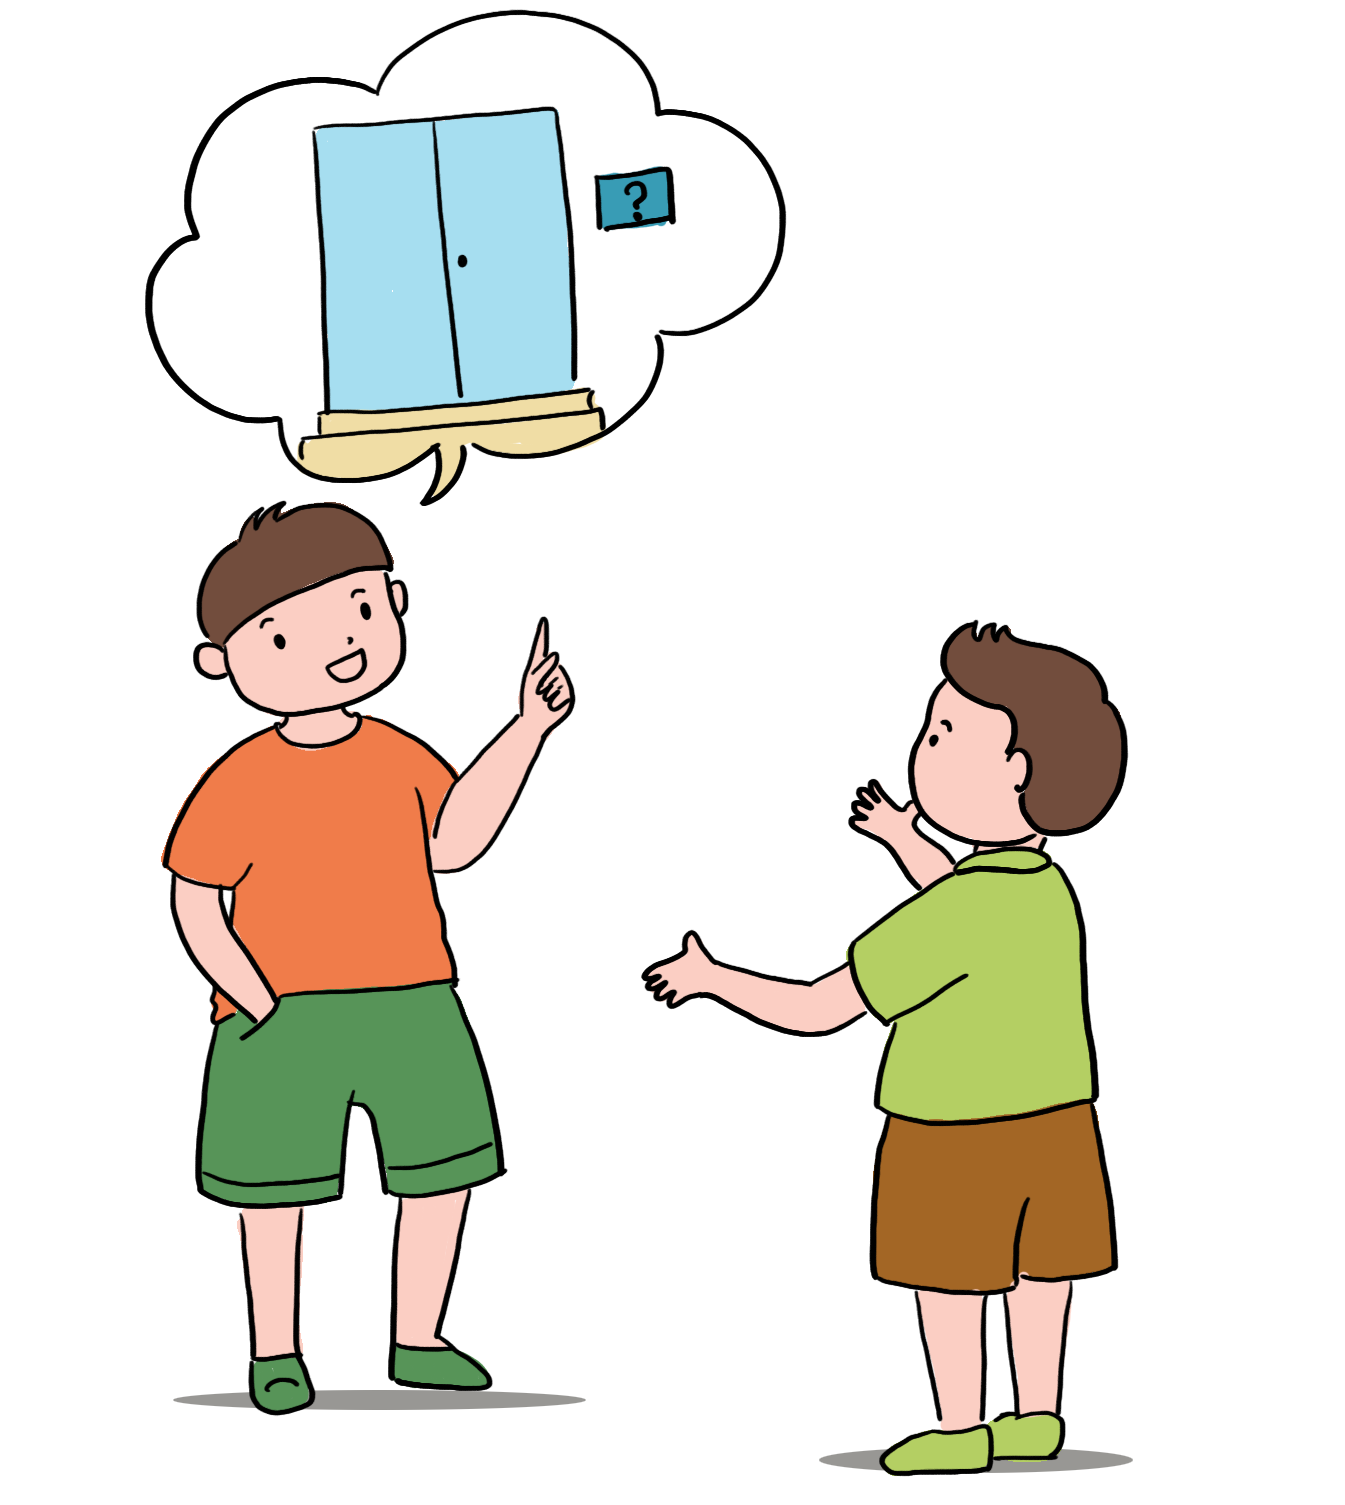
\includegraphics[width=1\linewidth]{Pi10_ToanBi_Bai3}
		\vspace*{-15pt}
	\end{figure}
	$\pmb{4.}$ Có $100$ chiếc thẻ bài bằng nhựa đánh số từ $1$ tới $100$ lần lượt được xếp thành hàng ngang. Cứ hai chiếc thẻ xếp cách nhau một chiếc thẻ khác đều có thể đổi chỗ được cho nhau. Liệu em có thể đổi chỗ các chiếc thẻ này bằng cách như trên để xếp lại được $100$ chiếc thẻ trên theo thứ tự ngược lại được hay không?
	\begin{figure}[H]
		\centering
		\vspace*{-5pt}
		\captionsetup{labelformat= empty, justification=centering}
		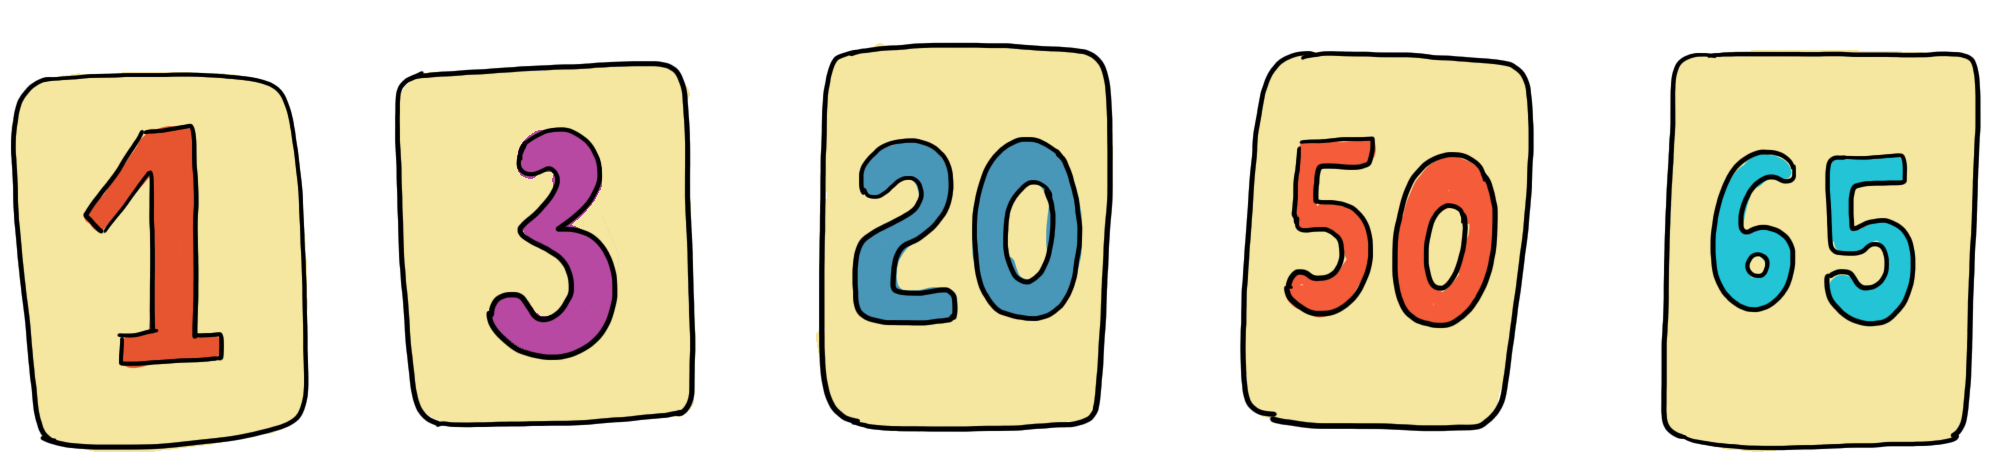
\includegraphics[width=1\linewidth]{Pi10_ToanBi_Bai4}
		\vspace*{-15pt}
	\end{figure}
	$\pmb{5.}$ Trong ngày khai giảng các bạn học sinh gặp lại nhau sau một mùa hè nên vô cùng mừng rỡ. Gặp lại bạn bè cũ và ai cũng tranh thủ bắt tay bạn mình. Kết thúc màn chào hỏi vui tươi sôi nổi, anh phụ trách thống kê lại trong cuốn sổ tổng số bạn học sinh đã có số lẻ lần bắt tay: tổng cộng là $67$ bạn. Bạn Lâm đứng cạnh anh phụ trách nói nhỏ ``Anh ơi, anh đếm nhầm rồi, chắc chắn không phải là $67$ bạn ạ". Anh phụ trách vô cùng ngạc nhiên, vì sao Lâm lại biết vậy. Em có thể giải thích vì sao Lâm lại cho rằng anh phụ trách đếm nhầm được không?
	\begin{figure}[H]
		\centering
%		\vspace*{-5pt}
		\captionsetup{labelformat= empty, justification=centering}
		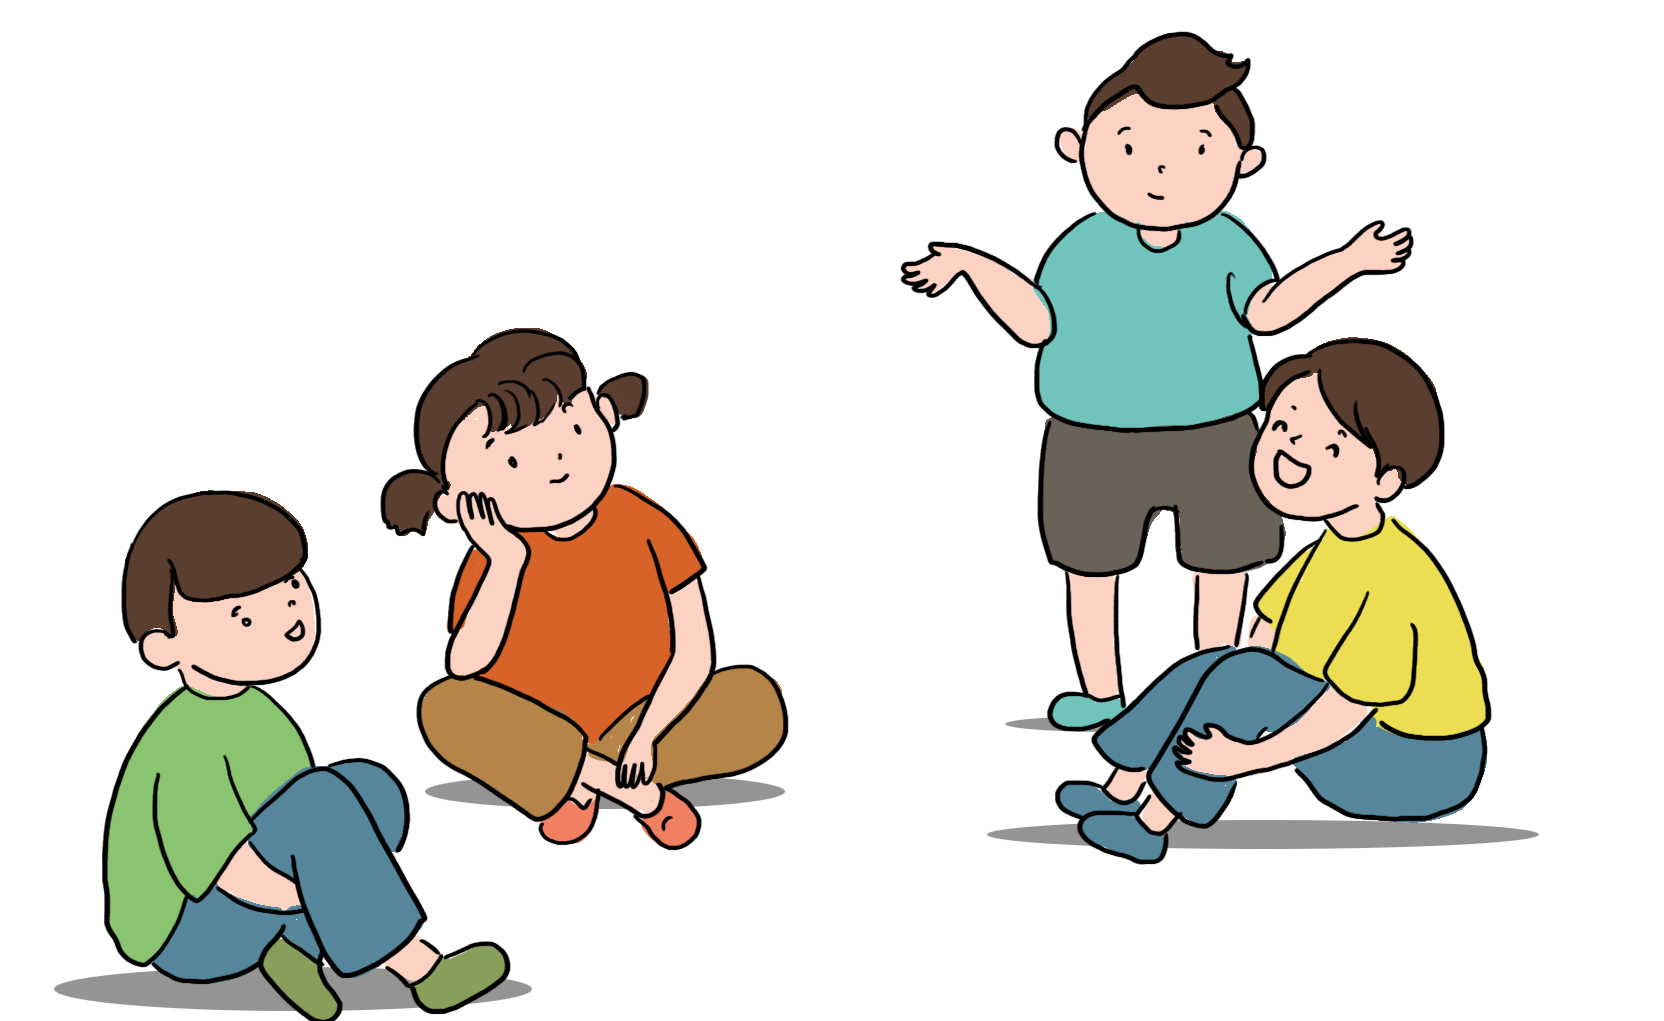
\includegraphics[width=1\linewidth]{Pi10_ToanBi_Bai5}
		\vspace*{-15pt}
	\end{figure}
	$\pmb{6.}$ $a)$  Có $50$ vị khách ngồi xung quanh một chiếc bàn tròn được xếp đều, trong số họ có $25$ phụ nữ. Em hãy chứng tỏ rằng có một vị khách ngồi cạnh hai phụ nữ.
	\vskip 0.1cm
	$b)$ Giả sử bây giờ số phụ nữ là $26$ người. Trong buổi tiệc bỗng dưng có hai vị khách làm vỡ mất hai chiếc cốc đặt trước mặt họ. Em hãy chứng tỏ rằng có thể xoay lại chiếc bàn tròn theo một cách nào đó để sao cho hai chiếc cốc vỡ lại đặt trước mặt của hai vị khách~nữ.
	\begin{figure}[H]
		\centering
		\vspace*{-10pt}
		\captionsetup{labelformat= empty, justification=centering}
		\includegraphics[width=1\linewidth]{Pi10_ToanBi_Bai6}
%		\vspace*{-5pt}
	\end{figure}
\end{multicols}
\vspace*{-10pt}
\rule{1\linewidth}{0.1pt}
\begingroup
\AddToShipoutPicture*{\put(112,374){\includegraphics[scale=1]{../tieude2.pdf}}} 
\centering
\endgroup
\graphicspath{{../toancuabi/pic/}}
\vspace*{75pt}

\begin{multicols}{2}
	$\pmb{1.}$ Hai bạn nhỏ tham gia trò chơi Nhà đầu tư nhỏ tuổi. Bạn Vinh nói với bạn Bình: ``Nếu $3/5$ số vốn của tớ mà được thêm $7000$ đồng, thì sẽ bằng số vốn của cậu". Nghe thế, Bình liền  nhận xét: ``Vậy là vốn của cậu chỉ hơn của tớ có $3000$ đồng." Các em hãy xác định số vốn của các bạn nhỏ này nhé.
	\begin{figure}[H]
		\vspace*{-10pt}
		\centering
		\captionsetup{labelformat= empty, justification=centering}
		\includegraphics[width= 1\linewidth]{bai1}
%		\vspace*{-5pt}
	\end{figure}
	\textit{Lời giải.} Số vốn tổng cộng của Vinh gồm $3/5$ phần vốn cộng với $2/5$ phần vốn. Nếu như Vinh thêm cả $7000$ vào số vốn của mình, thì Vinh  sẽ hơn Bình tận  $7000+3000= 10000$ (đồng). Từ đề bài ta thấy, do $3/5$ tiền vốn của Vinh cộng với $7000$ đồng đã bằng số vốn của Bình, nên $2/5$ số vốn của Vinh đúng bằng $10000$ (đồng). Vì thế số vốn của Vinh tham gia trò chơi là: $10000: (2/5)= 25000$ (đồng), và số vốn của Bình là $25000-3000=22000$ (đồng).
	\vskip 0.1cm
	$\pmb{2.}$ Có một số điểm dừng nghỉ cho người đi đường (nhiều hơn $1$) trải dọc trên một con đường dài $60$ km. Một người đi bộ dọc theo con đường với vận tốc $5$ (km$/$h) và nghỉ chân tại mỗi điểm dừng nghỉ cùng một khoảng thời gian là một số nguyên giờ đồng hồ. Một người khác đi xe đạp trên quãng đường đó với vận tốc $12$ (km$/$h) và nghỉ tại mỗi điểm dừng nghỉ với thời gian gấp đôi so với người đi bộ. Hai người cùng khởi hành và đến đích đồng thời. Hỏi có bao nhiêu điểm dừng nghỉ dọc trên đường.
	\begin{figure}[H]
		\vspace*{-8pt}
		\centering
		\captionsetup{labelformat= empty, justification=centering}
		\includegraphics[width= 1\linewidth]{bai2}
		\vspace*{-15pt}
	\end{figure}
	\textit{Lời giải.} Thời gian người đi bộ đi trên đường không tính thời gian nghỉ chân là $12$ giờ. Còn người đi xe đạp mất $5$ giờ để đạp xe. Vì thế thời gian người đi xe đạp nghỉ tại các gốc cây nhiều hơn số thời gian người đi bộ nghỉ là $12-5 = 7$ (giờ). Đây cũng chính là số tiếng người đi bộ đã nghỉ tại các điểm dừng nghỉ. Vì có nhiều hơn một điểm dừng nghỉ và khoảng thời gian nghỉ tại mỗi gốc là một lượng nguyên của giờ đồng hồ, nên suy ra có $7$ điểm dừng nghỉ trên đường.
	\vskip 0.1cm
	$\pmb{3.}$ Mãng xà hay có thói bắt trộm gà của dân làng. Một lần nọ nó bị đau bụng vì ăn nhiều thịt gà sống quá nên phải tới khám bác sỹ. Bác sỹ bảo nếu Mãng xà còn ăn tới $6$ con gà sống trong một ngày thì $10$ năm nữa nó sẽ chết, còn nếu ăn tận $17$ con gà một ngày như bây giờ thì chỉ còn sống được $5$ năm nữa. Hỏi Mãng xà sẽ sống được thêm bao nhiêu năm, nếu nó chịu khó không bắt gà ăn thịt lung tung nữa. (Ta coi rằng độ dài mỗi năm là như nhau và mỗi một con gà sống làm giảm tuổi thọ một số thời gian như nhau).
	\begin{figure}[H]
		\vspace*{-8pt}
		\centering
		\captionsetup{labelformat= empty, justification=centering}
		\includegraphics[width= 0.9\linewidth]{bai3}
		\vspace*{-5pt}
	\end{figure}
	\vskip 0.1cm
	Ta gọi số ngày trong năm là $n$. Khi đó $6\cdot10n= 60n$ là số gà ăn vào sẽ làm giảm tuổi thọ của Mãng xà để nó chỉ sống thêm được $10$ năm nữa. Còn $17\cdot5n = 85n$ là số gà ăn vào sẽ làm giảm tuổi thọ của Mãng xà để nó chỉ sống thêm được $5$ năm. Như vậy $85n-60n = 25n$ con gà sẽ làm giảm tuổi thọ của Mãng xà mất $5$ năm. Như vậy, nếu Mãng xà thôi không bắt gà sống ăn thịt thì nó sẽ sống thêm được $10$ năm cộng với số năm mà $60n$ con gà có thể đã tước đoạt đi tuổi thọ của nó, có nghĩa là $(60:25)\cdot5 = 12$ (năm).
	\vskip 0.1cm	
	Vậy nếu không bắt gà  của dân làng nữa, Mãng xà có thể sống thêm được $10+ 12 = 22$ (năm).
	\vskip 0.1cm
	$\pmb{4.}$ Có thể đặt các số tự nhiên từ $1$ tới $15$ vào một bảng vuông hình chữ nhật $3\times 5$ sao cho tổng các số trong mỗi hàng là như nhau và tổng các số trong mỗi cột cũng như nhau được hay không?
	\vskip 0.1cm
	Có thể. ta đưa ra một ví dụ như sau
	\begin{figure}[H]
		\centering
		\vspace*{-5pt}
		\captionsetup{labelformat= empty, justification=centering}
		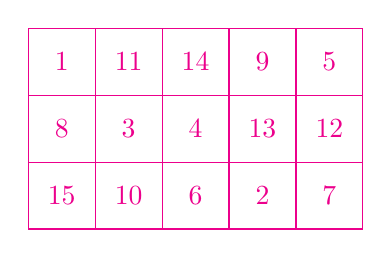
\begin{tikzpicture}[toancuabi,scale=0.85]
			\draw (0,0) grid (5,3);
			\node at (0.5,0.5) {$15$};
			\node at (1.5,0.5) {$10$};
			\node at (2.5,0.5) {$6$};
			\node at (3.5,0.5) {$2$};
			\node at (4.5,0.5) {$7$};
			\node at (0.5,1.5) {$8$};
			\node at (1.5,1.5) {$3$};
			\node at (2.5,1.5) {$4$};
			\node at (3.5,1.5) {$13$};
			\node at (4.5,1.5) {$12$};
			\node at (0.5,2.5) {$1$};
			\node at (1.5,2.5) {$11$};
			\node at (2.5,2.5) {$14$};
			\node at (3.5,2.5) {$9$};
			\node at (4.5,2.5) {$5$};
		\end{tikzpicture}
		\vspace*{-5pt}
	\end{figure}
	Sau đây là một số gợi ý:
	\vskip 0.1cm
	-- Trước tiên ta biết tổng của $15$ số bằng $(15\times16):2=120$. Do đó tổng của mỗi cột (nếu xếp được) là $24$, còn tổng mỗi hàng bằng $40$. Theo suy nghĩ thông thường ta chọn $3$ số cách đều $1$, $8$, $15$ cho cột đầu tiên.
	\vskip 0.1cm
	-- Xem xét $5$ số lớn nhất còn lại ta thấy $10$ và $11$ phải cùng một cột và cùng với số $3$. Ta xếp ba số $3$, $10$, $11$ vào cột hai (tạm thời chưa xếp vào các dòng). 
	\vskip 0.1cm
	-- Tiếp theo, trong các ô ở $3$ cột còn lại (cột thứ $3$ tới cột thứ $5$) ta sẽ xếp số lớn nhất $(14)$ cùng hàng với $1$ và số bé nhất $(2)$ cùng hàng với $15$ (cũng theo nguyên tắc xếp dãn đều). Thấy ngay $14$ và $2$ không thể ở cùng một cột, vì nếu như vậy, ô còn lại phải ghi số $8$ là số ta đã xếp ở cột $1$. Quay lại cột $2$, bằng cách xét từng trường hợp ta chỉ có thể  xếp số $3$ vào ô $G$ (Hình $1$).
	\begin{table}[H]
		\vspace*{-5pt}
		\centering
		\captionsetup{labelformat= empty, justification=centering}
		\renewcommand{\arraystretch}{1.23}
		\begin{tabular}{|c|c|c|c|c|}
			\hline
			$1$ & & $14$& & \\
			$A$&$B$&$C$&$D$& $E$\\
			\hline
			 $8$&$3$&&&\\
			 $F$&$G$&$H$&$I$&$J$\\
			 \hline
			 $15$&&&$2$&\\
			 $K$&$L$&$M$&$N$&$P$\\
			 \hline
		\end{tabular}
		\caption{\small\textit{\color{toancuabi}Hình $1$.}}
		\vspace*{-10pt}
	\end{table}
	-- Tiếp theo do tổng các ô $H$, $I$ và $J$ sẽ bằng $40-(8+3)= 29$ các ô này phải có cả hai số ``lớn" còn lại là $12$ và $13$ và ô còn lại trong $3$ ô này phải là số $4$. Xét $3$ trường hợp cho ô $I$ ta thấy chỉ có thể điền $13$ vào ô $I$.  Khi đó ta điền tiếp được các ô $H$, $J$, $D$, $M$ (Hình $2$)
	\begin{table}[H]
		\vspace*{-5pt}
		\centering
		\captionsetup{labelformat= empty, justification=centering}
		\renewcommand{\arraystretch}{1.23}
		\begin{tabular}{|c|c|c|c|c|}
			\hline
			$1$ & & $14$&$9$ & \\
			$A$&$B$&$C$&$D$& $E$\\
			\hline
			$8$&$3$&$4$&$13$&$12$\\
			$F$&$G$&$H$&$I$&$J$\\
			\hline
			$15$&&$6$&$2$&\\
			$K$&$L$&$M$&$N$&$P$\\
			\hline
		\end{tabular}
		\caption{\small\textit{\color{toancuabi}Hình $2$.}}
		\vspace*{-10pt}
	\end{table}
	-- Chỉ có thể điền $11$ vào ô $B$ và cuối cùng thu được toàn bộ bảng ở Hình $3$.
	\begin{table}[H]
		\vspace*{-5pt}
		\centering
		\captionsetup{labelformat= empty, justification=centering}
		\renewcommand{\arraystretch}{1.23}
		\begin{tabular}{|c|c|c|c|c|}
			\hline
			$1$ &$11$&$14$&$9$&$5$ \\
			$A$&$B$&$C$&$D$& $E$\\
			\hline
			$8$&$3$&$4$&$13$&$12$\\
			$F$&$G$&$H$&$I$&$J$\\
			\hline
			$15$&$10$&$6$&$2$&$7$\\
			$K$&$L$&$M$&$N$&$P$\\
			\hline
		\end{tabular}
		\caption{\small\textit{\color{toancuabi}Hình $3$.}}
		\vspace*{-10pt}
	\end{table}
	Các em cũng có thể đổi chỗ các cột, hoặc các hàng để có một cách điền khác.
	\vskip 0.1cm
	$\pmb{5.}$ Hai bạn cùng chơi một trò tô màu sau đây: các bạn lần lượt tô bằng màu đỏ các ô của một bảng ô vuông ca--rô $4\times 4$. Ở mỗi một bước, các bạn phải tô một ô trắng bằng màu đỏ, sao cho không có hình vuông $2\times 2$ nào bị tô đỏ hết. Bạn nào không đi được bước tiếp theo sẽ bị thua. Hỏi bạn nào sẽ luôn có cách chơi để thắng đối phương: bạn tô đầu tiên hay là người chơi cùng với bạn đó? 
	\begin{figure}[H]
		\vspace*{-5pt}
		\centering
		\captionsetup{labelformat= empty, justification=centering}
		\includegraphics[width= 1\linewidth]{bai5}
		\vspace*{-15pt}
	\end{figure}
	\textit{Lời giải.} Ta đánh số $16$ ô của bàn cờ caro như sau
	\begin{figure}[H]
		\centering
		\vspace*{-5pt}
		\captionsetup{labelformat= empty, justification=centering}
		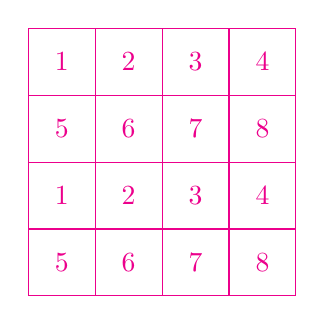
\begin{tikzpicture}[toancuabi,scale=0.85]
			\draw (0,0) grid (4,4);
			\node at (0.5,0.5) {$5$};
			\node at (1.5,0.5) {$6$};
			\node at (2.5,0.5) {$7$};
			\node at (3.5,0.5) {$8$};
			\node at (0.5,1.5) {$1$};
			\node at (1.5,1.5) {$2$};
			\node at (2.5,1.5) {$3$};
			\node at (3.5,1.5) {$4$};
			\node at (0.5,2.5) {$5$};
			\node at (1.5,2.5) {$6$};
			\node at (2.5,2.5) {$7$};
			\node at (3.5,2.5) {$8$};
			\node at (0.5,3.5) {$1$};
			\node at (1.5,3.5) {$2$};
			\node at (2.5,3.5) {$3$};
			\node at (3.5,3.5) {$4$};
		\end{tikzpicture}
		\vspace*{-5pt}
	\end{figure}
	Người chơi thứ hai (đối thủ của người đi trước) sẽ luôn có thể thắng bằng chiến thuật sau đây: hễ người thứ nhất tô màu vào ô nào trong số $16$ ô trong bảng, người chơi thứ hai sẽ tô vào ô có cùng số với ô vừa được người thứ nhất đã tô. Do không có hình vuông $2\times2$ nào trong bàn cờ có $2$ số giống nhau nên người thứ hai không bao giờ bị đẩy vào tình huống thua vì không đi được bước tiếp theo.
	\vskip 0.1cm
	$\pmb{6.}$ Có $31$ người cùng ngồi xung quanh một chiếc bàn tròn. Một số người trong họ là các Hiệp sỹ -- đó là những người luôn nói thật, còn những người còn lại là Lừa dối -- họ luôn nói sai, hơn nữa số người Lừa dối ít nhất là $1$. Người ta hỏi mỗi người trong số họ ``có bao nhiêu người Lừa dối ngồi cạnh anh?" (tức là người ngồi cạnh bên tay trái và bên tay phải). Tất cả mọi người cùng đưa ra câu trả lời như nhau. Hỏi số Hiệp sỹ lớn nhất có thể ngồi xung quanh bàn là bao nhiêu?
	\begin{figure}[H]
		\vspace*{-5pt}
		\centering
		\captionsetup{labelformat= empty, justification=centering}
		\includegraphics[width= 1\linewidth]{bai6}
		\vspace*{-10pt}
	\end{figure}
	\textit{Lời giải.} Giả sử xung quanh bàn có ít nhất $16$ Hiệp sỹ. Khi đó phải có ít  nhất $2$ Hiệp sỹ ngồi cạnh nhau. Hơn nữa vì số người Lừa dối có ít nhất là $1$, nên phải có $2$ Hiệp sỹ ngồi cạnh nhau, và một trong số họ có một người Lừa dối ngồi cạnh. Như vậy, có một Hiệp sỹ đưa ra câu trả lời là ``$1$", và tất cả cũng đã đều trả lời là ``$1$".
	\vskip 0.1cm 
	Vì thế các Hiệp sỹ phải ngồi theo từng cặp, mỗi một cặp Hiệp sỹ được bao quanh bởi các người Lừa dối. Hơn nữa, mỗi một người Lừa dối phải được bao quanh bởi $2$ Hiệp sỹ (vì nếu có một người Lừa dối có $2$ người ngồi cạnh là Hiệp sỹ và Lừa dối khác, thì hóa ra anh ta lại nói thật, điều này là không thể. Do đó chỉ có thể có cách xếp như sau
	\begin{align*}
		\ldots\text{\scriptsize{HHLHHLHHL}}\ldots
	\end{align*}
	(H -- Hiệp sỹ, L -- Lừa dối). Nhưng khi đó thì tổng số người phải là bội số của $3$. Đây là điều mâu thuẫn. Do vậy số Hiệp sỹ không quá $15$.
	\vskip 0.1cm
	Ta sẽ chỉ ra ví dụ khi có đúng $15$ Hiệp sỹ ngồi quanh bàn như sau
	\begin{align*}
		\text{\scriptsize{LHLHLHLHLHLHLHLHLHLHLHLHLHLHLLH}}
	\end{align*}
	(người đầu và người cuối trong dãy trên ngồi cạnh nhau). Khi đó mỗi người ở quanh bàn đều trả lời ``$2$".
\end{multicols}
\newpage
\begingroup
\thispagestyle{toancuabinone}
\blfootnote{$^1$\color{toancuabi}Trường THCS Archimedes, Hà Nội.}
\AddToShipoutPicture*{\put(60,733){\includegraphics[width=17.2cm]{../mathc.pdf}}}
%\AddToShipoutPicture*{\put(-2,733){\includegraphics[width=17.2cm]{../mathl.pdf}}} 
\AddToShipoutPicture*{\put(112,675){\includegraphics[scale=1]{../tieude3.pdf}}} 
\centering
\endgroup
\graphicspath{{../toancuabi/pic/}}
\vspace*{35pt}

\begin{multicols}{2}
	\PIbox{\textbf{\color{toancuabi}Problem} $\pmb{1.}$ How many ways are there to color the regions $A$, $B$, $C$, $D$ in the figure with three different colors, where each region is colored by one color?}	 
	\begin{figure}[H]
		\centering
		\vspace*{-5pt}
		\captionsetup{labelformat= empty, justification=centering}
		\includegraphics[scale=1]{m1}
		\vspace*{-5pt}
	\end{figure}
	\PIbox{\textbf{\color{toancuabi}Rule of Multiplication:} Suppose that we have to do two independent jobs $A$ and $B$, and that there are $m$ ways to do job $A$ and $n$ ways to do job $B$. We cannot do both jobs at the same time, then there are $(m \times n)$ ways to do \textbf{\color{toancuabi}both} jobs.}
	\vskip 0.1cm
	\textit{Solution}: There are $4$ regions to be colored, and there are $3$ ways to color each region. Therefore, the number of colorings is 
	\begin{align*}
		\text{Rule of multiplication: }	3 \times 3\times 3\times 3=81.
	\end{align*}
	\PIbox{\textbf{\color{toancuabi}Problem} $\pmb{2.}$ How many ways are there to color the regions $A$, $B$, $C$, $D$, $E$ in the figure using three different colors such that two adjacent regions have different colors?	} 
	\begin{figure}[H]
		\centering
		\vspace*{-5pt}
		\captionsetup{labelformat= empty, justification=centering}
		\includegraphics[scale=1]{m2}
		\vspace*{-10pt}
	\end{figure}
	\textit{Solution}: We color in the order $A \to B \to C \to D \to E$. There are $3$ ways to color region $A$. After that, there are $2$ ways to color $B$ with a different color. Then there are $2$ ways to color $C$ with a color different from $B$, and so on ...
	\vskip 0.1cm   
	According to the rule of multiplication, the number of colorings is given by
	\begin{align*}
		\text{Rule of multiplication: } 3 \times 2^4= 48.
	\end{align*}
	\PIbox{\textbf{\color{toancuabi}Problem} $\pmb{3.}$ How many ways are there to put $8$ rooks on a chessboard so that they do not attack each other? 
	\vskip 0.1cm
	(\textit{Note that two rooks on the same row or column attack each other.})}
	\begin{figure}[H]
		\centering
%		\vspace*{-5pt}
		\captionsetup{labelformat= empty, justification=centering}
		\includegraphics[width=1\linewidth]{co}
		\vspace*{-10pt}
	\end{figure}
	\textit{Solution}:
	\vskip 0.1cm 
	$\circ$ Step $1$: Put the $1^{\text{st}}$ rook on the $1^{\text{st}}$ row: $8$ ways
	\vskip 0.1cm
	$\circ$ Step $2$: Put the $2^{\text{nd}}$ rook on the $2^{\text{nd}}$ row: $7$ ways
	\vskip 0.1cm
	$\circ$ $\ldots$
	\vskip 0.1cm
	$\circ$ Step $8$: Put the $8^{\text{th}}$ rook on the $8^{\text{th}}$ row: $1$ way
	\vskip 0.1cm
	By the rule of multiplication, there are 
	\begin{align*}
		8\times7\times6\times\ldots\times1=40320
	\end{align*}
	ways to put $8$ rooks on a chessboard such that they do not attack each other.
	\vskip 0.1cm
	\PIbox{\textbf{\color{toancuabi}Problem} $\pmb{4.}$ There are $5$ {\color{green}green balls} numbered from $1$ to $5$, $6$ {\color{red}red balls} numbered from $1$ to $6$, and $7$ {\color{yellow}yellow balls} numbered from $1$ to $7$. How many ways are there to choose $3$ balls such that they have different colors and numbers?}
	\begin{figure}[H]
		\centering
		\vspace*{-5pt}
		\captionsetup{labelformat= empty, justification=centering}
		\includegraphics[width=1\linewidth]{bong}
		\vspace*{-10pt}
	\end{figure}
	\textit{Solution:}
	\vskip 0.1cm 
	$\circ$ First, we choose a {\color{green}green ball}. There are $5$ available choices. 
	\vskip 0.1cm
	$\circ$ Next, we choose a {\color{red}red ball}. The number on this {\color{red}red ball} is different from that of the {\color{green}green ball}, so there are $6-1=5$ available choices. 
	\vskip 0.1cm
	$\circ$ Finally, we choose a {\color{yellow}yellow ball}, and there are $7-2=5$ available choices. 
	\vskip 0.1cm
	According to the rule of multiplication, the number of ways to choose $3$ balls of different colors and different numbers is: 
	\begin{align*}
		5\times5\times5=125.
	\end{align*}
	\PIbox{\textbf{\color{toancuabi}Problem} $\pmb{5.}$ How many even $4$--digit numbers with distinct digits are there?}
	\vskip 0.1cm
	\textit{Solution}:  Let’s write an even $4$--digit number as $\overline{abcd}$ where $a\ne 0$, the $4$ digits $a$, $b$, $c$, $d$ are pairwise distinct, and $d$ is in the set $\{0,2,4,6,8\}$.
	\vskip 0.1cm
	We consider two cases:
	\vskip 0.1cm
	\textit{Case} $1$: $d=0$. There are $9$ ways to choose $a$, then $8$ ways to choose $b$ and then $7$ ways to choose $c$. Therefore, there are $1\times 9\times8\times7$ choices of the number $\overline{abcd}$.
	\vskip 0.1cm
	\textit{Case} $2$: $d\ne0$. There are $4$ ways to choose $d$. For each choice of $d$, there are $8$ ways to choose $a$ ($a\ne0$ and $a\ne d$), then $8$ ways to choose $b$ and then $7$ ways to choose $c$. Therefore, there are $4
	\times8\times8\times7$ choices of the number $\overline{abcd}$.
	\vskip 0.1cm
	Thus, there are 
	\begin{align*}
		1\times9\times8\times7+4\times8\times8\times7 = 2296
	\end{align*}
	numbers that satisfy the requirement of the problem.
	\vskip 0.1cm
	\PIbox{\textbf{\color{toancuabi}Exercise} $\pmb{1.}$ How many ways are there to color the regions $A$, $B$, $C$, $D$ in the figure with one color for each region, given that there are three different colors and no two adjacent regions have the same color?}
	\begin{figure}[H]
		\centering
		\vspace*{-5pt}
		\captionsetup{labelformat= empty, justification=centering}
		\includegraphics[scale=1]{m3}
		\vspace*{-5pt}
	\end{figure}
	\vskip 0.1cm
	\PIbox{\textbf{\color{toancuabi}Exercise} $\pmb{2.}$ How many ways are there to color the sides of a pentagon with three different colors such that no two adjacent sides have the same color?}
	\vskip 0.2cm
	\PIbox{{\centerline{\textbf{\color{toancuabi}New words}}}
		\vskip 0.2cm
		{\color{toancuabi}Adjacent(adj):} bên cạnh, cạnh nhau
		\vskip 0.1cm
		{\color{toancuabi}Case:} trường hợp 
		\vskip 0.1cm
		{\color{toancuabi}Color (v):} tô màu 
		\vskip 0.1cm
		{\color{toancuabi}Different:} khác 
		\vskip 0.1cm
		{\color{toancuabi}Region:} vùng, miền
		\vskip 0.1cm
		{\color{toancuabi}Rook (Chess):} quân Xe trên bàn cờ Vua  
		\vskip 0.1cm
		{\color{toancuabi}Rule of Multiplication:} Quy tắc Nhân
		\vskip 0.1cm
		{\color{toancuabi}Way:} con đường, cách (thực hiện) }
\end{multicols}
	\newpage
	
%	\setcounter{figure}{0}
%	\thispagestyle{thachthuctoanhocnone}
\pagestyle{thachthuctoanhoc}
\everymath{\color{thachthuctoanhoc}}
\graphicspath{{../thachthuctoanhoc/pic/}}
\begingroup
\AddToShipoutPicture*{\put(0,616){\includegraphics[width=19.3cm]{../thachthuctoanhoc/bannerthachthuc}}}
\centering
\vspace*{4cm}
\endgroup
\vspace*{-8pt}
\begin{tBox}
	\begin{itemize}[leftmargin = 13pt, itemsep = 1.0pt] 
				\item Mỗi bài toán đề xuất (kèm theo lời giải) cần được nêu rõ là bài sáng tác hay bài sưu tầm.
%		\item Mỗi bài toán đề xuất (kèm theo lời giải) cần được nêu rõ là bài sáng tác hay bài sưu tầm (nếu là bài sưu tầm, cần ghi rõ nguồn).
		\item Bài giải cho mỗi bài toán cần được trình bày trong một file riêng hoặc
		một tờ giấy riêng.
%		\item  Người đề xuất bài toán hoặc gửi bài giải cho các bài toán trong mục ``Thách thức kỳ này" cần ghi rõ họ, đệm, tên và nơi làm việc/học tập, số điện thoại liên hệ. Nếu là học sinh (hoặc sinh viên) cần ghi rõ là học sinh lớp mấy (hoặc sinh viên năm thứ mấy).
%		\item Các bài toán trong mục Thách thức kỳ này hướng tới các độc giả là học sinh phổ thông; được phân chia thành các mức độ $B$, $A$, và được sắp xếp theo độ khó tăng dần, theo đánh giá chủ quan của Ban biên tập. Các bài toán mức độ $B$ không đòi hỏi các kiến thức vượt quá chương trình môn Toán cấp THCS; các bài toán mức độ $A$ không đòi hỏi các kiến thức vượt quá chương trình môn Toán cấp THPT.
%		\item Cách thức gửi bài toán đề xuất hoặc lời giải: gửi file thu được bằng cách scan, ảnh chụp (rõ nét) của bản viết tay, hoặc được soạn thảo bằng các phần mềm Latex, Word tới \url{bbt@pi.edu.vn} hoặc gửi qua đường bưu điện tới Tòa soạn (xem địa chỉ tại bìa $2$).
		\item Hạn gửi lời giải cho các bài toán P$641$--P$650$: trước ngày $15/11/2022$.
	\end{itemize}
\end{tBox}
\begin{center}
	\vspace*{-5pt}
	\textbf{\color{thachthuctoanhoc}\color{thachthuctoanhoc}THÁCH THỨC KỲ NÀY}
	\vspace*{-5pt}
\end{center}
\begin{multicols}{2}
	\setlength{\abovedisplayskip}{4pt}
	\setlength{\belowdisplayskip}{4pt}
	{\color{thachthuctoanhoc}{\usefont{T5}{qag}{b}{n} P641.}}
	(Mức $B$) Tại mỗi đỉnh của một đa giác lồi $18$ cạnh ở hình dưới đây, người ta ghi một số, sao cho số được ghi ở mỗi đỉnh bằng tổng hai số được ghi ở hai đỉnh kề với nó.
	\begin{figure}[H]
		\vspace*{-5pt}
		\centering
		\captionsetup{labelformat= empty, justification=centering}
		\definecolor{ffvvqq}{rgb}{1,0.3333333333333333,0}
		\definecolor{qqqqffa}{rgb}{0,0,1}
		\definecolor{qqzzff}{rgb}{0,0.6,1}
		\begin{tikzpicture}[line cap=round,line join=round,>=triangle 45,x=1cm,y=1cm,scale=0.4]
			\draw (1.401115339869085,5.50644760016908136) node[anchor=north west] {$X$};
			\draw (1.4408759814898973,-0.7306378725360659) node[anchor=north west] {$Y$};
			\draw (-7.8444170535279,2.5008856260029945) node[anchor=north west] {$S$};
			\draw [color=qqzzff] (0.0915547437082469,-1.9784020259611625)--(1.3147607160299626,-0.9781184915188108);
			\draw [color=qqzzff] (1.3147607160299626,-0.9781184915188108)--(2.122081224105652,0.3802016464606015); 
			\draw [color=qqzzff] (2.122081224105652,0.3802016464606015)--(2.4161414998796458,1.932724932666551); 
			\draw [color=qqzzff] (2.4161414998796458,1.932724932666551)--(2.1614735342261406,3.4921941459791768);
			\draw [color=qqzzff] (2.1614735342261406,3.4921941459791768)--(1.38879404230183,4.87051428395859);
			\draw [color=qqzzff] (1.38879404230183,4.87051428395859)--(0.19129957436757605,5.901439596125702);
			\draw [color=qqzzff] (0.19129957436757605,5.901439596125702)--(-1.2865743636076452,6.4606252749959765);
			\draw [color=qqzzff] (-1.2865743636076452,6.4606252749959765)--(-2.866574363607645,6.480625274995977);
			\draw [color=qqzzff] (-2.866574363607645,6.480625274995977)--(-4.358129107315893,5.959027300957139);
			\draw [color=qqzzff] (-4.358129107315893,5.959027300957139)--(-5.581335079637608,4.958743766514788);
			\draw [color=qqzzff] (-5.581335079637608,4.958743766514788)--(-6.388655587713298,3.600423628535374);
			\draw [color=qqzzff] (-6.388655587713298,3.600423628535374)--(-6.682715863487291,2.0479003423294264);
			\draw [color=qqzzff] (-6.682715863487291,2.0479003423294264)--(-6.428047897833785,0.4884311290167975);
			\draw [color=qqzzff] (-6.428047897833785,0.4884311290167975)--(-5.655368405909476,-0.889889008962613);
			\draw [color=qqzzff] (-5.655368405909476,-0.889889008962613)--(-4.457873937975224,-1.9208143211297237);
			\draw [color=qqzzff] (-4.457873937975224,-1.9208143211297237)--(-2.98,-2.48);
			\draw [color=qqzzff] (-2.98,-2.48)--(-1.4,-2.5);
			\draw [color=qqzzff] (-1.4,-2.5)--(0.0915547437082469,-1.9784020259611625);
			\draw [fill=qqqqffa] (-2.98,-2.48) circle (1.6pt);
			\draw [fill=qqqqffa] (-1.4,-2.5) circle (1.6pt);
			\draw [fill=qqqqffa] (0.0915547437082469,-1.9784020259611625) circle (1.6pt);
			\draw [fill=qqqqffa] (1.3147607160299626,-0.9781184915188108) circle (1.6pt);
			\draw [fill=qqqqffa] (2.122081224105652,0.3802016464606015) circle (1.6pt);
			\draw [fill=qqqqffa] (2.4161414998796458,1.932724932666551) circle (1.6pt);
			\draw [fill=qqqqffa] (2.1614735342261406,3.4921941459791768) circle (1.6pt);
			\draw [fill=qqqqffa] (1.38879404230183,4.87051428395859) circle (1.6pt);
			\draw [fill=qqqqffa] (0.19129957436757605,5.901439596125702) circle (1.6pt);
			\draw [fill=qqqqffa] (-1.2865743636076452,6.4606252749959765) circle (1.6pt);
			\draw [fill=qqqqffa] (-2.866574363607645,6.480625274995977) circle (1.6pt);
			\draw [fill=qqqqffa] (-4.358129107315893,5.959027300957139) circle (1.6pt);
			\draw [fill=qqqqffa] (-5.581335079637608,4.958743766514788) circle (1.6pt);
			\draw [fill=qqqqffa] (-6.388655587713298,3.600423628535374) circle (1.6pt);
			\draw [fill=qqqqffa] (-6.682715863487291,2.0479003423294264) circle (1.6pt);
			\draw [fill=qqqqffa] (-6.428047897833785,0.4884311290167975) circle (1.6pt);
			\draw [fill=qqqqffa] (-5.655368405909476,-0.889889008962613) circle (1.6pt);
			\draw [fill=qqqqffa] (-4.457873937975224,-1.9208143211297237) circle (1.6pt);
		\end{tikzpicture}
		\vspace*{-5pt}
	\end{figure}
	Biết rằng, số được ghi ở đỉnh $X$ là $20$, và số được ghi ở đỉnh $Y$ là $22$. Hãy tìm số được ghi ở đỉnh $S$. 
	\vskip 0.1cm
	\hfill	\textit{Bùi Văn Biên, France (st)}
	\vskip 0.1cm
	{\color{thachthuctoanhoc}{\usefont{T5}{qag}{b}{n} P642.}}
	(Mức $B$) Cho $x,y$ là các số nguyên dương thoả mãn $y^2+x-1$ chia hết cho \linebreak $xy+1$. Chứng minh rằng, tồn tại số tự nhiên $z$ sao cho $x+y+z+xyz$ là số chính phương.
	\vskip 0.1cm
		\hfill\textit{Nguyễn Đức Tấn, Tp. Hồ Chí Minh}
	\vskip 0.1cm
	{\color{thachthuctoanhoc}{\usefont{T5}{qag}{b}{n} P643.}}
	(Mức $B$) Người ta lần lượt ghi các số lên bảng, theo quy tắc: Ở mỗi lần ghi, chỉ ghi một số, và nếu số được ghi ở lần thứ $k$ ($k\in\mathbb N^*$) là $x\neq-1$, thì ở lần thứ $k+1$ ghi số $\dfrac{x-1}{x+1}$. Hãy tìm số nhỏ nhất cần ghi ở lần thứ nhất, sao cho trong quá trình ghi số lên bảng theo quy tắc trên, ta ghi được số $-\frac1{2023}$. 
	\vskip 0.1cm
	\hfill	\textit{Phùng Chí Tự, Hà Nội}
	\vskip 0.1cm
	{\color{thachthuctoanhoc}{\usefont{T5}{qag}{b}{n} P644.}}
	(Mức $B$) Xét tam giác $ABC$ có các góc $B,C$ nhọn. Gọi $H$ là chân đường cao kẻ từ $A$ của tam giác đó.  Chứng minh rằng $ABC$ là tam giác vuông tại $A$ khi và chỉ khi 
	\begin{align*}
		\dfrac{HB^3}{AB^4}+\dfrac{HC^3}{AC^4}=\dfrac1{BC}\cdot
	\end{align*} 
	\begin{figure}[H]
		\vspace*{-5pt}
		\centering
		\captionsetup{labelformat= empty, justification=centering}
		\definecolor{ffqqqq}{rgb}{1,0,0}
		\definecolor{qqzzff}{rgb}{0,0.6,1}
		\definecolor{qqqqff}{rgb}{0,0,1}
		\definecolor{qqqqffa}{rgb}{1,1,1}
		\definecolor{cqcqcq}{rgb}{0.7529411764705882,0.7529411764705882,0.7529411764705882}
		\begin{tikzpicture}[line cap=round,line join=round,>=triangle 45,x=1cm,y=1cm, scale=0.5]
			\draw (-2.8771572875253812,-2) -- (-2.8771572875253812,-1.7171572875253809) -- (-3.16,-1.7171572875253809) -- (-3.16,-2) -- cycle; 
			\draw [color=qqzzff] (-3.16,4.66)-- (-5.54,-2);
			\draw [color=qqzzff] (-5.54,-2)-- (2,-2);
			\draw [color=qqzzff] (2,-2)-- (-3.16,4.66);
			\draw [,color=ffqqqq] (-3.16,4.66)-- (-3.16,-2);
			\draw [fill=qqqqffa] (-3.16,4.66) circle (1.6pt);
			\draw[color=qqqqff] (-3.18,5.11) node {$A$};
			\draw [fill=qqqqffa] (-5.54,-2) circle (1.6pt);
			\draw[color=qqqqff] (-5.7,-2.5) node {$B$};
			\draw [fill=qqqqffa] (2,-2) circle (1.6pt);
			\draw[color=qqqqff] (2,-2.5) node {$C$};
			\draw [fill=qqqqffa] (-3.16,-2) circle (1.6pt);
			\draw[color=qqqqff] (-3.18,-2.5) node {$H$};
		\end{tikzpicture}
		\vspace*{-10pt}
	\end{figure}
	\vskip 0.05cm
		\hfill\textit{Trần Quang Hùng, Hà Nội}
	\vskip 0.05cm
	{\color{thachthuctoanhoc}{\usefont{T5}{qag}{b}{n} P645.}}
	(Mức $B$) Cho $a,b,c$ là các số thực dương thoả mãn $abc=1$. Chứng minh rằng 
	\begin{align*}
		\dfrac{a}{a\!+\!b^{3} c\!+\!b}+\dfrac{b}{b\!+\!c^{3} a\!+\!c}+\dfrac{c}{c\!+\!a^{3} b\!+a} \ge 1.
	\end{align*}
	\vskip 0.05cm
		\hfill\textit{Đào Văn Nam, Hà Nội}
	\vskip 0.05cm
	{\color{thachthuctoanhoc}{\usefont{T5}{qag}{b}{n} P646.}}
	(Mức $B$) Chứng minh rằng, trong mỗi bát giác lồi, luôn có ít nhất ba đường chéo mà độ dài của chúng đôi một khác nhau. 
	\vskip 0.05cm
	(Bát giác là một đa giác có $8$ cạnh.)
	\vskip 0.1cm
		\hfill \textit{Phạm Nhật Nguyệt, Hải Phòng}
	\vskip 0.1cm
	{\color{thachthuctoanhoc}{\usefont{T5}{qag}{b}{n} P647.}}
	(Mức $A$) Cho số nguyên $n \geq 2$, và cho $n$ điểm đôi một phân biệt $A_1, A_2, \ldots, A_n$ cùng nằm trên một đường tròn, theo thứ tự đó (tính theo chiều kim đồng hồ). Một dãy các điểm đôi một phân biệt $A_{k_1}$, $A_{k_2}, \ldots, A_{k_t}$ $(t \in\mathbb N, t \geq 2)$ được gọi là một {\it đường đi}, nếu đường gấp khúc $A_{k_1} A_{k_2} \ldots A_{k_t}$ ($t$ đỉnh) là một đường gấp khúc không tự cắt. Hỏi có tất cả bao nhiêu đường đi?
	\vskip 0.05cm
	(Một đường gấp khúc được gọi là {\it không tự cắt}, nếu không có hai cạnh nào của nó cắt nhau tại một điểm nằm bên trong mỗi cạnh, trong hai cạnh ấy.)
	\vskip 0.1cm
	\hfill	\textit{Nguyễn Tường Thanh, Nghệ An (st)}
	\vskip 0.1cm
	{\color{thachthuctoanhoc}{\usefont{T5}{qag}{b}{n} P648.}}
	(Mức $A$) Với mỗi số thực $a$, xét tất cả các hàm số $f: \mathbb R \rightarrow \mathbb R,$ thỏa mãn
	\begin{align*}
		f(a x+y+f(x+y))+f(x y)=y f(x)
	\end{align*}
	với mọi $x,y\in\mathbb R$.
	\vskip 0.05cm
	$a)$ Tìm tất cả các số thực $a$, sao cho trong các hàm số $f$, tồn tại một hàm là đơn ánh từ $\mathbb R$ đến $\mathbb R$.
	\vskip 0.05cm
	$b)$ Với $a=2$, tìm tất cả các hàm số $f$ có $f(0)=0$.
	\vskip 0.1cm
	\hfill		\textit{Lê Phúc Lữ, Tp. Hồ Chí Minh}
	\vskip 0.1cm
	{\color{thachthuctoanhoc}{\usefont{T5}{qag}{b}{n} P649.}}
	(Mức $A$) Cho tam giác $ABC$ và điểm $D$ cố định nằm trên cạnh $BC$ ($D$ khác $B,C$). Một đường tròn $(O)$ thay đổi, đi qua $B, C$ và cắt các cạnh $AB, AC$ tương ứng tại $E, F$ (khác $A,B,C$). Gọi $G$ là giao điểm của $BF$ và $AD$. Chứng minh rằng, đường thẳng $GE$ luôn đi qua một điểm cố định.
	\begin{figure}[H]
		\vspace*{-10pt}
		\centering
		\captionsetup{labelformat= empty, justification=centering}
		\definecolor{ffqqqq}{rgb}{1,0,0}
		\definecolor{qqzzff}{rgb}{0,0.6,1}
		\definecolor{qqqqff}{rgb}{0,0,1}
		\definecolor{qqqqffa}{rgb}{1,1,1}
		\begin{tikzpicture}[line cap=round,line join=round,>=triangle 45,x=1cm,y=1cm,scale=0.5]
			\draw [color=qqzzff] (-4.81309,-1)-- (-2.9915435035522586,4.9363824736365585);
			\draw [color=qqzzff] (-2.9915435035522586,4.9363824736365585)-- (2.16949,-1);
			\draw [color=qqzzff] (2.16949,-1)-- (-4.81309,-1);
			\draw [thachthuctoanhoc] (-1.3218,-0.16393583791880353) circle (3.590001273985364cm);
			\draw [] (-4.81309,-1)-- (-1.6642556805547637,3.409694424723417);
			\draw [] (-2.9915435035522586,4.9363824736365585)-- (-0.3604269142578283,-1);
			\draw [,color=ffqqqq] (-6.227177601372653,1.9518434021508382)-- (2.997592242483252,3.9372366050655776);
			\draw [fill=qqqqffa] (-2.9915435035522586,4.9363824736365585) circle (1.6pt);
			\draw[color=qqqqff] (-3.0725009370690106,5.432246753926664) node {$A$};
			\draw [fill=qqqqffa] (-4.81309,-1) circle (1.6pt);
			\draw[color=qqqqff] (-5.177394208504555,-1.1455447193094175) node {$B$};
			\draw [fill=qqqqffa] (2.16949,-1) circle (1.6pt);
			\draw[color=qqqqff] (2.531407750174166,-1.2062627944469815) node {$C$};
			\draw [fill=qqqqffa] (-1.3218,-0.16393583791880353) circle (1.6pt);
			\draw[color=qqqqff] (-1.721554748380367,-0.3966884592794637) node {$O$};
			\draw [fill=qqqqffa] (-3.7432966215398427,2.4864345624380344) circle (1.6pt);
			\draw[color=qqqqff] (-4.064229497649219,2.801130164632231) node {$E$};
			\draw [fill=qqqqffa] (-1.6642556805547637,3.409694424723417) circle (1.6pt);
			\draw[color=qqqqff] (-1.5545490586299158,3.873816158729192) node {$F$};
			\draw [fill=qqqqffa] (-0.3604269142578283,-1) circle (1.6pt);
			\draw[color=qqqqff] (-0.36042691425782825,-1.507459586342921) node {$D$};
			\draw [fill=qqqqffa] (-2.0657079453674543,2.847492151010585) circle (1.6pt);
			\draw[color=qqqqff] (-2.161729810005554,2.11658235542766) node {$G$};
		\end{tikzpicture}
		\vspace*{-10pt}
	\end{figure}
	\hfill	\textit{Phạm Vĩnh Minh, Đồng Tháp}
	\vskip 0.1cm
	{\color{thachthuctoanhoc}{\usefont{T5}{qag}{b}{n} P650.}}
	(Mức $A$) Cho $p$ là một số nguyên tố có dạng $4k+3$, $k\in\mathbb N$.  Xét dãy số Fibonacci $(F_n)$, xác định bởi: $F_0=0$, $F_1=1$, và 
	\begin{align*}
		F_{n+2}=F_{n+1}+F_n\quad\text{\color{black}với mọi } n\ge0.
	\end{align*}
	Chứng minh rằng, không tồn tại các số nguyên dương $m,n$, với $n\ge 5$, sao cho \linebreak$F_n=p^m$.
	\vskip 0.1cm
	\hfill	\textit{Nguyễn Song Minh, Hà Nội (st)}
	\vskip 0.1cm
\end{multicols}
	\begin{center}
		{\large{\textbf{\color{thachthuctoanhoc}GIẢI BÀI KỲ TRƯỚC}}}
	\end{center}
\begin{multicols}{2}
	\setlength{\abovedisplayskip}{4pt}
	\setlength{\belowdisplayskip}{4pt}
	{\color{thachthuctoanhoc}{\usefont{T5}{qag}{b}{n} P621.}}
	(Mức $B$) Xét ba số nguyên tố có tổng bằng $242$. Hỏi,  tích của chúng lớn nhất bằng bao nhiêu?
	\vskip 0.05cm
	\textbf{Lời giải} (\textit{dựa theo cách giải của bạn Võ Trần Tiến, lớp $8^5$, trường THCS Long Bình Điền, tỉnh Tiền Giang})\textbf{.}
	\vskip 0.05cm
	Ta biết rằng, tổng của ba số nguyên dương là một số chẵn khi và chỉ khi trong ba số đó, có đúng một số chẵn, hoặc cả ba số đều là số chẵn. Vì thế, do $242$ là số chẵn và do chỉ có đúng một số nguyên tố chẵn, là $2$, nên trong ba số nguyên tố thỏa mãn điều kiện đề bài, phải có một số là $2$, và hai số còn lại là hai số lẻ. Gọi hai số lẻ này là $a$, $b$, và kí hiệu $T$ là tích của ba số được xét; ta có
	\begin{align*}
		a + b = 242 - 2 = 240,                          \tag{$1$}
	\end{align*}
	và $T = 2ab$.
	\vskip 0.05cm
	Không mất tính tổng quát, giả sử $a \ge b$. Khi đó, $a + b \le 2a$; kết hợp với ($1$), suy ra, $a \ge 120$. Mà $a$ là số nguyên tố và $120$ không là số nguyên tố, nên ta có $a > 120$. Do đó, đặt $a = 120 + m$, ta có $m$ là số nguyên dương lẻ (do $a$ là số lẻ), và
	\begin{align*}
		b = 240 - a = 240 - (120 + m) = 120 - m.
	\end{align*}
	Suy ra, $T = 2\left( {120 + m} \right)\left( {120 - m} \right) = 2\left( {{{120}^2} - {m^2}} \right).$ \hfil ($2$)
	\vskip 0.05cm
	Do đó, $T$ lớn nhất khi $m$ là số nguyên dương lẻ nhỏ nhất, sao cho $120 + m$ và $120 - m$ cùng là số nguyên tố.
	\vskip 0.05cm
	Với $m = 1, 3, 5$, ta có $120 + m = 121, 123, 125$, đều là hợp số (do  $121 \vdots 11$, $123  \vdots  3$  và  $125 \vdots 5$).
	\vskip 0.05cm
	Với $m = 7$, ta có $120 + m = 127$, là số nguyên tố; đồng thời, $120 - m = 113$, cũng là số nguyên tố.
	\vskip 0.05cm
	Vì vậy, $T$ lớn nhất khi $m = 7$. Do đó, theo ($2$), giá trị lớn nhất của $T$ bằng
	\begin{align*}
		2\left( {{{120}^2} - {7^2}} \right) = 28702.
	\end{align*}
	Ta có điều phải tìm theo yêu cầu đề bài.
	\vskip 0.05cm
	\textbf{Bình luận và Nhận xét}
	\vskip 0.05cm	
	$\pmb{1.}$ Có thể thấy, ngoài bộ $(2, 113, 127)$, còn có nhiều bộ ba số nguyên tố có tổng bằng $242$; chẳng hạn, các bộ $(2, 7, 233)$, $(2, 11, 229)$, $(2, 13, 227)$, $(2, 17, 223)$, $\ldots$ . Vì thế, câu hỏi đặt ra ở đề bài là có nghĩa.
	\vskip 0.05cm
	$\pmb{2.}$ Dựa vào một số ý đã nêu ở Lời giải trên, bạn đọc có thể dễ dàng tìm ra \textit{tất cả} các bộ ba số nguyên tố có tổng bằng $242$.
	\vskip 0.05cm
	$\pmb{3.}$ Rất tiếc, trong số các lời giải Tạp chí nhận được từ bạn đọc, có một lời giải sai (tuy có đáp số đúng), do người giải bài đã khẳng định tích $T$ (theo kí hiệu ở Lời giải trên đây) lớn nhất, khi ba số nguyên tố là $2$, $113$, $127$, mà không có bất cứ lời giải thích hợp lí nào. Bên cạnh lời giải sai này, còn có một lời giải không được coi là lời giải hoàn chỉnh, do người giải bài chưa khẳng định được $113$ và $127$ là các số nguyên tố thỏa mãn điều kiện đã đặt ra ở lời giải của mình, để tích $T$ là lớn nhất.
	\vskip 0.05cm
	\hfill \textbf{Lê Huy}
	\vskip 0.05cm
	{\color{thachthuctoanhoc}{\usefont{T5}{qag}{b}{n} P622.}}
	(Mức $B$) Cho $x,y,z$ là các số thực khác $0$ thoả mãn 
	\begin{align*}
		\dfrac{x^2+y}{y^2}=\dfrac{y^2+z}{z^2}=\dfrac{z^2+x}{x^2}=2.
	\end{align*}
	Chứng minh rằng, $\dfrac x{y^2}+\dfrac y{z^2}+\dfrac z{x^2}$ là một số nguyên.
	\vskip 0.05cm
	\textbf{Lời giải} ()\textbf{.}
	\vskip 0.05cm
	\textbf{Bình luận và Nhận xét}
	\vskip 0.05cm
	\hfill\textbf{Lê Huy}
	\vskip 0.05cm
	(Mức $B$) Mỗi ô của bảng ô vuông kích thước $2023\times2023$. Ban đầu mỗi ô của bảng ghi số $1$. Người ta thực hiện việc ghi xoá và ghi thêm số theo quy tắc sau: mỗi lần chọn ra $3$ ô trong cùng một hàng hoặc một cột; mỗi ô được chọn, nếu ô đó đang ghi số $N$, người ta xoá đi và ghi số $N+1$ vào ô đó. 
	\vskip 0.05cm
	Hỏi sau một số hữu hạn lần thực hiện ghi và xoá số như vậy, người ta có thể làm cho tất cả các số được ghi trong bảng là các số chẵn được hay không?
	\textbf{Lời giải} (\textit{dựa theo Đáp án do BBT Tạp chí cung cấp})\textbf{.}
	\vskip 0.05cm
	Xét một hàng tùy ý của bảng đã cho. Lần lượt, từ trái qua phải, đánh số thứ tự các ô vuông con của hàng này, bởi $1, 2, \ldots, 2023$. Ta gọi ô vuông con có số thứ tự $i$ là ô $i$.
	\vskip 0.05cm
	Thực hiện phép thay đổi số đối với các ô vuông con của hàng nêu trên, như sau:
	\vskip 0.05cm
	-- Với mỗi $k = 1, 2, \ldots, 673$, ở lần thực hiện thứ $k$, thay đổi số, theo qui tắc của đề bài, ở ba ô $3k - 2$, $3k - 1$, $3k$;
	\vskip 0.05cm
	-- Ở lần thực hiện thứ $674$, thay đổi số ở ba ô $2019$, $2020$, $2021$;
	\vskip 0.05cm
	-- Ở lần thực hiện thứ $675$, thay đổi số ở ba ô $2019$, $2022$, $2023$.
	\vskip 0.05cm
	Khi đó, do ban đầu, ở mỗi ô của hàng đang xét có một số $1$, nên sau $673$ lần thực hiện đầu tiên, ở mỗi ô, từ ô $1$ đến ô $2019$, có một số $2$, và ở mỗi ô $2020$, $2021$, $2022$, $2023$ có một số $1$. Do đó, sau lần thực hiện thứ $674$, ở ô $2019$ có một số $3$, ở mỗi ô $2022$, $2023$ có một số $1$, và ở mỗi ô còn lại của hàng có một số $2$. Vì vậy, sau lần thực hiện thứ $675$, ở ô $2019$ có một số $4$, và ở mỗi ô còn lại có một số $2$.
	\vskip 0.05cm
	Như vậy, với qui trình thực hiện nêu trên, sau $675$ lần thực hiện liên tiếp phép thay đổi số của đề bài, ta có thể làm cho tất cả các số ở tất cả các ô của một hàng tùy ý đều là số chẵn. Vì thế, nhờ việc thực hiện liên tiếp một số hữu hạn lần phép thay đổi số của đề bài đối với bảng đã cho, ta có thể nhận được bảng $2023 \times 2023$, mà số ở mỗi ô vuông con của nó đều là số chẵn.
	\vskip 0.05cm
	\textbf{Bình luận và Nhận xét}
	\vskip 0.05cm
	$\pmb{1.}$ Từ lời giải trên dễ thấy, \textit{câu trả lời} cho câu hỏi của bài đã ra \textit{không thay đổi}, nếu thay bảng $2023 \times 2023$ bởi bảng $(3n + 1) \times (3n + 1)$, với $n$ là một số nguyên dương tùy ý lớn hơn $1$.
	\vskip 0.05cm
	$\pmb{2.}$ Từ điều vừa nêu trên, hiển nhiên xuất hiện câu hỏi: \textit{Nếu ở bài đã ra, thay bảng $2023 \times 2023$ bởi bảng $4 \times 4$, thì câu trả lời cho câu hỏi đặt ra ở bài toán là gì?} Mời bạn đọc tìm câu trả lời cho câu hỏi vừa nêu.
	\vskip 0.05cm
	$\pmb{3.}$ Rất tiếc, cho tới thời điểm bản thảo vào Nhà in, Tạp chí vẫn chưa nhận được một lời giải nào, từ bạn đọc.
	\vskip 0.05cm
	\hfill\textbf{Nguyễn Khắc Minh}
	\vskip 0.05cm
	{\color{thachthuctoanhoc}{\usefont{T5}{qag}{b}{n} P624.}}
	(Mức $B$) Cho tam giác $ABC$ nhọn, nội tiếp đường tròn $(O)$. Các đường cao xuất phát từ các đỉnh $B,C$ của tam giác, tương ứng, cắt $(O)$ tại các điểm thứ hai $P,Q$. Gọi $M$ là trung điểm của cạnh $BC$, và gọi $K, L$ tương ứng là hình chiếu vuông góc của $M$ trên $AC, A B$. Các đường thẳng $Q L, P K$ cắt đường thẳng $B C$ tương ứng tại $R, S$. Chứng minh rằng, bốn điểm $P, Q, R, S$ cùng nằm trên một đường tròn.
	\vskip 0.05cm
	\textbf{Lời giải} (\textit{dựa theo đa số lời giải Tạp chí đã nhận được từ bạn đọc})\textbf{.}
	
	%%
	Do tam giác $ABC$ nhọn, nên $P$ thuộc cung $AC$ không chứa $B$, và $Q$ thuộc cung $AB$ không chứa $C$, của $(O)$. Do đó, $A$, $P$, $Q$ nằm cùng phía đối với đường thẳng $BC$. \hfill ($1$)
	\vskip 0.05cm
	Gọi $E$ và $F$ tương ứng là chân đường cao kẻ từ $B$ và $C$ của tam giác $ABC$.
	\vskip 0.05cm
	Vì cùng vuông góc với $AC$ nên $MK \parallel BE$, và vì cùng vuông góc với $AB$ nên $ML \parallel BF$. Mà $M$ là trung điểm của $BC$ (giả thiết), nên suy ra, $K$, $L$ tương ứng là trung điểm của $CE$, $BF$. \hfill ($2$)
	\vskip 0.05cm
	Từ ($1$) và ($2$) suy ra, các điểm $R$, $S$ nằm giữa $B$ và $C$. \hfill ($3$)
	\vskip 0.05cm
	Do ($1$) nên từ việc xét đường tròn $(O)$, ta có:
	\begin{align*}
		\angle BQF = \angle BQC = \angle BAC = \angle BPC = \angle CPE.
	\end{align*}
	Vì thế, tam giác vuông $BFQ$ đồng dạng với tam giác vuông $CEP$. Kết hợp với ($2$), suy ra
	\begin{align*}
		\frac{{FQ}}{{EP}} = \frac{{FB}}{{EC}} = \frac{{FL}}{{EK}}.
	\end{align*}
	Do đó, tam giác vuông $LFQ$ đồng dạng với tam giác vuông $KEP$. Suy ra
	\begin{align*}
		\angle CQR = \angle FQL = \angle EPK = \angle BPS. \tag{$4$}
	\end{align*}
	Do $BCPQ$ là tứ giác nội tiếp nên với lưu ý tới ($3$), ta có:
	\begin{align*}
		\angle RCQ = \angle BCQ = \angle BPQ. \tag{$5$}
	\end{align*}
	Từ ($4$) và ($5$), với lưu ý tới ($3$), suy ra
	\begin{align*}
		\angle BRQ = \angle CQR + \angle RCQ = \angle BPS + \angle BPQ = \angle SPQ.
	\end{align*}
	Do đó, $RSPQ$ là tứ giác nội tiếp, hay bốn điểm $P$, $Q$, $R$, $S$ cùng nằm trên một đường tròn.
	\vskip 0.05cm
	Ta có điều phải chứng minh theo yêu cầu đề bài.
	\vskip 0.05cm
	\textbf{Bình luận và Nhận xét}
	\vskip 0.05cm
	Tất cả các lời giải Tạp chí nhận được từ bạn đọc đều là lời giải đúng và hoàn chỉnh.
	\vskip 0.05cm
	\hfill \textbf{Hạ Vũ Anh}
	\vskip 0.05cm
	{\color{thachthuctoanhoc}{\usefont{T5}{qag}{b}{n} P625.}}
	(Mức $B$) Cho các số thực dương $a,b,c$. Chứng minh rằng
	\begin{align*}
		\left(\dfrac b{a+c}\right)^2+\left(\dfrac{c}{a+b}\right)^2\ge \dfrac{b^2-bc+c^2}{a^2+bc}.
	\end{align*}
	\textbf{Lời giải} (\textit{của người chấm bài})\textbf{.}
	\vskip 0.05cm
	Do $a, b, c > 0$ nên theo bất đẳng thức Cauchy -- Schwarz, ta có:
	\begin{align*}
		{\left( {a + c} \right)^2} = {\left( {a \cdot 1 + \sqrt {bc}  \cdot \frac{{\sqrt c }}{{\sqrt b }}} \right)^2} \le \left( {{a^2} + bc} \right)\left( {\frac{c}{b} + 1} \right) = \frac{{\left( {{a^2} + bc} \right)\left( {b + c} \right)}}{b}.
	\end{align*}
	Suy ra
	\begin{align*}
		\frac{{{b^2}}}{{{{\left( {a + c} \right)}^2}}} \ge \frac{{{b^3}}}{{\left( {{a^2} + bc} \right)\left( {b + c} \right)}}. \tag{$1$}
	\end{align*}
	Bằng cách hoàn toàn tương tự, ta cũng chứng minh được:
	\begin{align*}
		\frac{{{c^2}}}{{{{\left( {a + b} \right)}^2}}} \ge \frac{{{c^3}}}{{\left( {{a^2} + bc} \right)\left( {b + c} \right)}}. \tag{$2$}
	\end{align*}
	Cộng ($1$) với ($2$), vế theo vế, ta được:
	\begin{align*}
		{\left( {\frac{b}{{a + c}}} \right)^2} + {\left( {\frac{c}{{a + b}}} \right)^2} \ge \frac{{{b^3} + {c^3}}}{{\left( {{a^2} + bc} \right)\left( {b + c} \right)}} = \frac{{{b^2} - bc + {c^2}}}{{{a^2} + bc}}.
	\end{align*}
	Bất đẳng thức của đề bài được chứng minh.
	\vskip 0.05cm
	\textbf{Bình luận và Nhận xét}
	\vskip 0.05cm
	$\pmb{1.}$ Dễ thấy, dấu đẳng thức ở bất đẳng thức của đề bài xảy ra khi và chỉ khi $a = b = c$.
	\vskip 0.05cm
	$\pmb{2.}$ Bằng phương pháp của lời giải trên, ta có thể chứng minh được kết quả sau:
	\vskip 0.05cm
	``\textit{Với a, b, c là các số thực dương, ta có:}
	\vskip 0.05cm
	$i)$  $\frac{1}{{{{\left( {a + b} \right)}^2}}} + \frac{1}{{{{\left( {a + c} \right)}^2}}} \ge \frac{1}{{{a^2} + bc}}$;
	\vskip 0.05cm
	$ii)$  $\frac{1}{{a + b}} + \frac{1}{{b + c}} + \frac{1}{{c + a}} \ge \frac{a}{{{a^2} + bc}} + \frac{b}{{{b^2} + ca}} + \frac{c}{{{c^2} + ab}}.$"
	\vskip 0.05cm
	$\pmb{3.}$ Sử dụng bất đẳng thức $i)$ trên đây, ta có thể giải được bài toán bất đẳng thức trong Đề thi chọn đội tuyển Trung Quốc dự thi $IMO$ năm $2004$. Bài toán đó như sau:
	\vskip 0.05cm
	``\textit{Cho các số thực dương $x$, $y$, $z$, $t$ thỏa mãn $xyzt = 1$. Chứng minh rằng}
	\begin{align*}
		\frac{1}{{{{\left( {x + 1} \right)}^2}}} + \frac{1}{{{{\left( {y + 1} \right)}^2}}} + \frac{1}{{{{\left( {z + 1} \right)}^2}}} + \frac{1}{{{{\left( {t + 1} \right)}^2}}} \ge 1. \text{\color{black}"}
	\end{align*}
	$\pmb{4.}$ Số lời giải Tạp chí nhận được từ bạn đọc không nhiều. Trong số này, rất tiếc, chỉ có hai lời giải đúng; các lời giải còn lại bị sai do người giải bài đã mắc một trong các lỗi cơ bản dưới đây:
	\vskip 0.05cm
	-- Áp dụng phép chuẩn hóa cho bất đẳng thức không thuần nhất;
	\vskip 0.05cm
	-- Từ $0 < x \le y$ suy ra  $\dfrac{1}{x} \le \dfrac{1}{y}$.
	\vskip 0.05cm 
	\hfill \textbf{Võ Quốc Bá Cẩn}
	\vskip 0.05cm
	{\color{thachthuctoanhoc}{\usefont{T5}{qag}{b}{n} P626.}}
	(Mức $B$) Xét các tam giác vuông mà độ dài các cạnh là các số nguyên dương và một trong các cạnh góc vuông có độ dài là $2021^{22}$. Hỏi có bao nhiêu tam giác như vậy? 
	\vskip 0.05cm
	\textbf{Lời giải} (\textit{của người chấm bài})\textbf{.}
	\vskip 0.05cm
	Trong phần trình bày dưới đây, $|X|$ kí hiệu số phần tử của tập hữu hạn $X$.
	\vskip 0.05cm
	Kí hiệu $x$ là độ dài cạnh huyền và $y$ là độ dài cạnh góc vuông còn lại của tam giác vuông thỏa mãn điều kiện đề bài. Khi đó, $x$, $y$ là các số nguyên dương, $x > y$, và
	\begin{align*}
		{\left( {{{2021}^{22}}} \right)^2} + {y^2} = {x^2}. \tag{$1$}
	\end{align*}
	Hiển nhiên, số tam giác thỏa mãn điều kiện đề bài chính bằng số cặp số nguyên dương $(x, y)$ thỏa mãn $x > y$ và ($1$). \hfill ($2$)
	\vskip 0.05cm
	Ta có
	\begin{align*}
		(1) \Leftrightarrow \left( {x - y} \right)\left( {x + y} \right) = {2021^{44}}. \tag{$3$}
	\end{align*}
	Do đó, số cặp số nguyên dương $(x, y)$ thỏa mãn $x > y$ và ($1$) bằng số cặp số nguyên dương $(x, y)$ thỏa mãn $x > y$ và ($3$). \hfill ($4$)
	\vskip 0.05cm
	Dưới đây, ta sẽ gọi cặp số nguyên dương thỏa mãn các điều kiện vừa nêu trên là \textit{cặp số thuận}.
	\vskip 0.05cm
	Xét một cặp số thuận tùy ý. Vì $x > y > 0$ nên  $0 < x - y < x + y$. Do đó
	\begin{align*}
		\left( {x - y} \right)\left( {x + y} \right) > {\left( {x - y} \right)^2};
	\end{align*}
	kết hợp với ($3$), suy ra $x - y < 2021^{22}$. Vì thế, từ ($3$) ta có $x - y$ là một ước dương nhỏ hơn $2021^{22}$  của $2021^{44}$. Do đó, phép đặt ứng
	\begin{align*}
		\text{``cặp số thuận } (x, y) \mapsto   d = x - y\text{"}
	\end{align*}
	sẽ xác lập một ánh xạ, gọi là $f$, từ tập $T$ gồm tất cả các cặp số thuận đến tập $S$ gồm tất cả các ước dương nhỏ hơn $2021^{22}$  của $2021^{44}$.
	\vskip 0.05cm 
	Với $\left( {{x_1},{y_1}} \right),\left( {{x_2},{y_2}} \right)$  tùy ý thuộc $T$, và $\left( {{x_1},{y_1}} \right) \ne \left( {{x_2},{y_2}} \right)$, dễ thấy, ta có ${x_1} - {y_1} \ne {x_2} - {y_2}$  (vì nếu ngược lại,  ${x_1} - {y_1} = {x_2} - {y_2}$, thì theo ($3$), sẽ có  ${x_1} + {y_1} = {x_2} + {y_2}$; dẫn đến $x_1 = x_2$  và  $y_1 = y_2$, mâu thuẫn với giả thiết  $\left( {{x_1},{y_1}} \right) \ne \left( {{x_2},{y_2}} \right)$). Do đó,  $f$ là một đơn ánh từ $T$ đến $S$. \hfill  ($5$)
	\vskip 0.05cm
	Với $d$ tùy ý thuộc $S$, xét cặp số $(x, y)$, xác định bởi:
	\begin{align*}
		x = \frac{1}{2}\left( {d + \frac{{{{2021}^{44}}}}{d}} \right) \text{\color{black} và } y = \frac{1}{2}\left( {\frac{{{{2021}^{44}}}}{d} - d} \right)
	\end{align*}
	Ta có
	\begin{align*}
		\left( {x - y} \right)\left( {x + y} \right) = d \cdot \frac{{{{2021}^{44}}}}{d} = {2021^{44}}. \tag{$6$}
	\end{align*}
	Vì $d \in S$ và $2021^{44}$  là một số lẻ nên $x, y \in \mathbb{N^*}$,  và $x > y$. Từ đây và ($6$), suy ra $(x, y) \in T$.
	\vskip 0.05cm
	Do $x - y = d$ nên $d$ là ảnh của $(x, y)$ qua  $f$. Vì thế,  $f$ là một toàn ánh từ $T$ đến $S$. \hfill ($7$)
	\vskip 0.05cm
	Từ ($6$) và ($7$) suy ra,  $f$ là một song ánh từ $T$ đến $S$. Do đó, $|T| = |S|$.
	\vskip 0.05cm 
	Vì ứng với mỗi ước dương nhỏ hơn $2021^{22}$  của $2021^{44}$  có đúng một ước dương lớn hơn $2021^{22}$  của  $2021^{44}$, ứng với mỗi ước dương lớn hơn $2021^{22}$   của  $2021^{44}$ có đúng một ước dương nhỏ hơn $2021^{22}$  của  $2021^{44}$, và $2021^{22}$  là một ước dương của  $2021^{44}$, nên
	\begin{align*}
		|S| = \frac{{N - 1}}{2},
	\end{align*}
	trong đó, $N$ là số ước dương của $2021^{44}$.
	\vskip 0.05cm
	Vì ${2021^{44}} = {43^{44}} \cdot {47^{44}}$ là phân tích chuẩn của $2021^{44}$, nên
	\begin{align*}
		N = \left( {44 + 1} \right)\left( {44 + 1} \right) = 2025.
	\end{align*}
	Do đó
	\begin{align*}
		|S| = \frac{{2025 - 1}}{2} = 1012.
	\end{align*}
	Vì vậy,  $|T| = 1012$. Từ đây và ($4$), ($2$), ta có số tam giác cần tìm theo yêu cầu đề bài là $1012$.
	\vskip 0.05cm
	\textbf{Bình luận và Nhận xét}
	\vskip 0.05cm
	$\pmb{1.}$ Lập luận ``Từ $x - y$ là một ước dương nhỏ hơn $2021^{22}$  của  $2021^{44}$, và với mỗi ước dương nhỏ hơn $2021^{22}$  của $2021^{44}$  xác định được ít nhất một cặp số thuận (theo ``định nghĩa" trong lời giải trên), suy ra, số cặp số thuận bằng số ước dương nhỏ hơn   của  " là một lập luận sai kiến thức cơ bản; vì lập luận đó tương đương với khẳng định ``nếu tồn tại một toàn ánh từ tập $X$ đến tập $Y$ thì  $|X| = |Y|$".
	\vskip 0.05cm
	$\pmb{2.}$ Trong số các lời giải Tạp chí đã nhận được từ bạn đọc, rất tiếc, có một lời giải sai (do người giải bài đếm ``thừa", vì quên rằng $20216{22}$  là một ước dương của  $2021^{44}$) và một lời giải không hoàn chỉnh (do người giải bài lập luận thiếu chặt chẽ, thiếu chính xác).
	\vskip 0.05cm
	\hfill \textbf{Hà Thanh}
	\vskip 0.05cm
	{\color{thachthuctoanhoc}{\usefont{T5}{qag}{b}{n} P627.}}
	(Mức $A$) Xét $x,y$ là hai số thực dương thoả mãn $xy\ge 1$. Tìm giá trị lớn nhất của biểu thức
	\begin{align*}
		P=\dfrac1{\sqrt{x^2+1}}+\dfrac1{\sqrt{y^2+1}}-\dfrac3{4(x+y)}.
	\end{align*}
	\textbf{Lời giải} (\textit{dựa theo lời giải của bạn Trần Minh Hoàng, lớp $10$T$1$, trường THPT chuyên Hà Tĩnh, tỉnh Hà Tĩnh})\textbf{.}
	\vskip 0.05cm
	Đặt $a = \frac{1}{{\sqrt {{x^2} + 1} }}$  và  $b = \frac{1}{{\sqrt {{y^2} + 1} }}$; ta có $a, b > 0$, và $P$ được viết lại dưới dạng:
	\begin{align*}
		P = a + b - \frac{3}{{4\left( {x + y} \right)}}. \tag{$1$}
	\end{align*}
	Áp dụng bất đẳng thức Cauchy -- Schwarz cho hai bộ số thực $(x, 1)$ và $(1, y)$, ta được:
	\begin{align*}
		{\left( {x + y} \right)^2} \le \left( {{x^2} + 1} \right)\left( {{y^2} + 1} \right);
	\end{align*}
	suy ra
	\begin{align*}
		\frac{1}{{x + y}} \ge \frac{1}{{\sqrt {\left( {{x^2} + 1} \right)\left( {{y^2} + 1} \right)} }} = ab (\text{\color{black}do } x,y >0) \tag{$2$}
	\end{align*}
	Từ ($1$) và ($2$), ta có
	\begin{align*}
		P \le a + b - \frac{3}{4}ab. \tag{$3$}
	\end{align*}
	Vì $xy \ge 1$ nên
	\begin{align*}
		{a^2} + {b^2} = \frac{1}{{{x^2} + 1}} + \frac{1}{{{y^2} + 1}} = \frac{{{x^2} + {y^2} + 2}}{{\left( {{x^2} + 1} \right)\left( {{y^2} + 1} \right)}} = \frac{{{x^2} + {y^2} + 2}}{{{{\left( {x + y} \right)}^2} + {{\left( {xy - 1} \right)}^2}}} \le \frac{{{{\left( {x + y} \right)}^2}}}{{{{\left( {x + y} \right)}^2} + {{\left( {xy - 1} \right)}^2}}} \le 1.
	\end{align*}
	Do đó, ${\left( {a + b} \right)^2} \le 2ab + 1$; suy ra
	\begin{align*}
		ab \ge \frac{1}{2}{\left( {a + b} \right)^2} - \frac{1}{2}.
	\end{align*}
	Từ ($3$) và ($4$), ta được:
	\begin{align*}
		P \le a + b - \frac{3}{8}{\left( {a + b} \right)^2} + \frac{3}{8} = \frac{{25}}{{24}} - {\left( {a + b - \frac{4}{3}} \right)^2} \le \frac{{25}}{{24}}.
	\end{align*}
	Hơn nữa, với  $x = \frac{{9 - 4\sqrt 2 }}{7}$ và  $y = \frac{{9 + 4\sqrt 2 }}{7}$, ta có $x, y > 0, xy = 1$, và bằng tính toán trực tiếp, dễ dàng tính được  $P = \dfrac{25}{24}$.
	\vskip 0.05cm
	Vì vậy, giá trị lớn nhất của $P$ bằng  $\dfrac{25}{24}$.
	\vskip 0.05cm
	\textbf{Bình luận và Nhận xét}
	\vskip 0.05cm
	$\pmb{1.}$ Các giá trị $x, y$ ở phần cuối của Lời giải trên được tìm ra từ việc xét khả năng xảy ra dấu đẳng thức ở các bất đẳng thức trong lời giải.
	\vskip 0.05cm
	$\pmb{2.}$ Rất tiếc, trong số các lời giải Tạp chí nhận được từ bạn đọc, có một lời giải sai, do người giải bài đã nhầm lẫn trong các đánh giá.
	\vskip 0.05cm
	\hfill\textbf{Lưu Thị Thanh Hà}
	\vskip 0.05cm
	{\color{thachthuctoanhoc}{\usefont{T5}{qag}{b}{n} P628.}}
	(Mức $A$) Cho tam giác không cân $ABC$ ngoại tiếp đường tròn $(I)$. Gọi $A_1$, $B_1$, $C_1$ tương ứng là tiếp điểm của $BC$, $CA$, $AB$ với $(I)$; $A_2$, $B_2$, $C_2$ lần lượt là đối xứng của $A_1$, $B_1$, $C_1$ tương ứng qua các đường thẳng $B_1C_1$, $C_1A_1$ và $A_1B_1$. Các đường thẳng $AA_2$, $BC$ cắt nhau tại $A_3$; $BB_2$ và $CA$ cắt nhau tại $B_3$; $CC_2$ và $AB$ cắt nhau tại $C_3$. Chứng minh rằng, $A_3$, $B_3$, $C_3$ thẳng hàng.
	\vskip 0.05cm
	\textbf{Lời giải} (\textit{của người chấm bài})\textbf{.}
	
	%%
	Gọi $H$ là trực tâm của tam giác $A_1B_1C_1$.
	\vskip 0.05cm 
	Vì tam giác $ABC$ không cân nên nó không là tam giác đều. Suy ra, $A_1B_1C_1$  là tam giác không đều; do đó,  $H \not\equiv I$.
	\vskip 0.05cm
	Do $A_1H \bot B_1C_1$  và  $A_1A_2 \not B_1C_1$, nên $H$ nằm trên đường thẳng  $A_1A_2$.
	\vskip 0.05cm
	Gọi $L$, $A_4$  tương ứng là giao điểm của đường thẳng $AI$ và  $B_1C_1$, $BC$.
	\vskip 0.05cm
	Do tam giác $ABC$ không cân tại $A$, nên $I$ không nằm trên đường thẳng $AA_1$; do đó, $A_4 \not\equiv A_1$    \hfill ($1$)
	\vskip 0.05cm 
	Theo tính chất của hai tiếp tuyến cắt nhau của một đường tròn,  $Ai \bot B_1C_1$; suy ra:
	\vskip 0.05cm
	-- $L$ là trung điểm của $B_1C_1$, \hfill ($2$)
	\vskip 0.05cm
	-- $A_1A_2 \parallel A_4A$  (do cùng vuông góc với  $B_1C_1$ và ($1$)). \hfill($3$)
	\vskip 0.05cm
	Từ ($2$), do $H$, $I$ tương ứng là trực tâm, tâm đường tròn ngoại tiếp tam giác  $A_1B_1C_1$, suy ra
	\begin{align*}
		A_1H = 2IL. \tag{$4$}
	\end{align*}
	Do  $IC_1 \bot AB, IA \bot B_1C_2$, và  $\angle IAC_1, \angle IC_1L$ là các góc nhọn, nên $\angle IAC_1 = \angle IC_1L]$. Do đó, tam giác vuông (tại  $C_1$) $AC_1I$   đồng dạng với tam giác vuông (tại $L$) $C_1LI$.  Suy ra
	\begin{align*}
		\frac{{AI}}{{{C_1}I}} = \frac{{{C_1}I}}{{LI}}.\tag{$5$}
	\end{align*}
	Gọi $M$ là điểm đối xứng với $A_1$  qua $I$. Từ ($5$) và ($4$), ta có:
	\begin{align*}
		\frac{{AI}}{{{C_1}I}} = \frac{{{A_1}M}}{{{A_1}H}} \tag{$6$}
	\end{align*}
	Gọi $K$ là giao điểm của $A_1A_2$ và  $B_1C_1$; gọi $N$ là giao điểm thứ hai (khác $A_1$) của  $A_1A_2$ và đường tròn ($I$).
	\vskip 0.05cm
	Do $A_1, A_2$  đối xứng với nhau qua  $B_1C_1$ nên $K$ là trung điểm $A_1A_2$;  mặt khác, do $H$ là trực tâm tam giác $A_1B_1C_1$, và  $HN \bot B_1C_1$, nên $K$ là trung điểm $HN$. Suy ra, $A_1H = A_2N$; do đó, $A_1N = A_2H$. \hfill  ($7$)
	\vskip 0.05cm
	Từ ($3$) suy ra  $\angle MA_1N = \angle A_4IA_1$; do đó, tam giác vuông (tại  $A_1$) $IA_1A_4$ đồng dạng với tam giác vuông (tại $N$) $A_1NM$.  Suy ra
	\begin{align*}
		\frac{{I{A_1}}}{{{A_1}N}} = \frac{{I{A_4}}}{{{A_1}M}}. \tag{$8$}
	\end{align*}
	Nhân ($6$) với ($8$), vế theo vế, ta được
	\begin{align*}
		\frac{{AI}}{{{A_1}N}} = \frac{{I{A_4}}}{{{A_1}H}};
	\end{align*}
	suy ra,  $\frac{{AI}}{{I{A_4}}} = \frac{{{A_1}N}}{{{A_1}H}}$. Kết hợp với ($7$), ta được:
	\begin{align*}
		\frac{{AI}}{{I{A_4}}} = \frac{{{A_2}H}}{{H{A_1}}}.
	\end{align*}
	Từ đây và ($3$), theo định lí Thales, suy ra, ba điểm  $A_3$, $H$, $I$ thẳng hàng; nói một cách khác, $A_3$  nằm trên đường thẳng $HI$.
	\vskip 0.05cm
	Bằng cách hoàn toàn tương tự, ta cũng chứng minh được, các điểm $B_3, C_3$  nằm trên đường thẳng $HI$. Vì thế, ba điểm  $A_3, B_3 ,C_3$  thẳng hàng.
	\vskip 0.05cm
	\textbf{Bình luận và Nhận xét}
	\vskip 0.05cm
	$\pmb{1.}$ Với giả thiết tam giác $ABC$ cân, chẳng hạn tại $A$, \textit{nhưng không đều}, ta có  $A_3 \equiv A_4$ và bốn điểm đôi một phân biệt $A$, $H$, $I$, $A_1$  thẳng hàng. Do vậy, trong trường hợp này,  $A_3$ vẫn nằm trên đường thẳng $HI$. Vì thế, từ lời giải trên dễ thấy, khẳng định của bài ra vẫn đúng, khi thay giả thiết ``không cân" bởi giả thiết (``nhẹ nhàng" hơn) ``\textit{không đều}".
	\vskip 0.05cm
	$\pmb{2.}$ Bài đã ra (với việc thay giả thiết ``không cân" bởi giả thiết ``không đều") là một kết quả hay, thú vị về đường thẳng Euler của một tam giác. Kết quả này đã được Lev Emelyanov công bố trong bài báo ``On the Intercepts of the OI -- Line", đăng trên Forum Geometricorum, Vol. 4, năm 2004 (trang 81 - 84).
	Forum Geometricorum là một Tạp chí về Hình học Euclid cổ điển và các lĩnh vực liên quan, được ấn hành bởi Đại học Atlantic Florida. Bạn đọc có thể tìm đọc Tạp chí này online, tại trang web \url{http://forumgeom.fau.edu.}
	\vskip 0.05cm
	$\pmb{3.}$ Tất cả lời giải Tạp chí nhận được, từ bạn đọc, đều là lời giải đúng.
	\vskip 0.05cm
	\hfill	\textbf{Hạ Vũ Anh}
	\vskip 0.05cm
	{\color{thachthuctoanhoc}{\usefont{T5}{qag}{b}{n} P629.}}
	(Mức $A$) Cho $n$ là một số nguyên dương có tính chất: không tồn tại các số nguyên dương $a,b,c$ sao cho $\dfrac4n=\dfrac 1a+\dfrac 1b+\dfrac 1c.$ Chứng minh rằng, tồn tại các số nguyên không âm $u,v$ sao cho: $n=u^2+v^2$.  
	\vskip 0.05cm
	\textbf{Lời giải} (\textit{phỏng theo lời giải của bạn Hồ Trần Khánh Linh, lớp $12$ Toán $2$, trường THPT chuyên ĐHSP, ĐHSP Hà Nội})\textbf{.}
	\vskip 0.05cm
	Trong Lời giải này, ta qui ước gọi một số nguyên dương là \textit{số tốt}, nếu nó biểu diễn được dưới dạng tổng bình phương của hai số nguyên không âm.
	\vskip 0.05cm
	Trước hết, dễ thấy $n = 1$ là một số nguyên dương có tính chất đã nêu trong đề bài, vì $\dfrac{4}{1} = 4$ và với mọi $a, b, c$ nguyên dương, $\frac{1}{a} + \frac{1}{b} + \frac{1}{c} \le 3$.
	\vskip 0.05cm
	Do  $1 = 0^2 + 1^2$, nên $n = 1$ là một số tốt. \hfill ($1$)
	\vskip 0.05cm
	Xét $n > 1$.
	\vskip 0.05cm
	Ta có hai Nhận xét sau:
	\vskip 0.05cm
	\textbf{Nhận xét} $\pmb{1:}$ \textit{$n$ không thể là số chẵn}, vì nếu ngược lại, $n$ là số chẵn, thì chọn  $a= \dfrac{n}{2}$, $b = c = n$, ta sẽ có $a,b,c \in \mathbb{N^*}$  và
	\begin{align*}
		\frac{1}{a} + \frac{1}{b} + \frac{1}{c} = \frac{2}{n} + \frac{1}{n} + \frac{1}{n} = \frac{4}{n}.
	\end{align*}
	\textbf{Nhận xét} $\pmb{2:}$ $n$ \textit{không thể có ước nguyên tố dạng} $4k + 3$, $k \in \mathbb{N}$, vì nếu ngược lại, $n$ có ước nguyên tố $p$ có dạng đó, thì chọn  $a = \frac{{n\left( {p + 1} \right)}}{4}$,  $b = c = \frac{{n\left( {p + 1} \right)}}{{2p}}$, ta sẽ có $a,b,c \in \mathbb{N^*}$  và
	\begin{align*}
		\frac{1}{a} + \frac{1}{b} + \frac{1}{c} = \frac{4}{{n\left( {p + 1} \right)}} + \frac{{2p}}{{n\left( {p + 1} \right)}} + \frac{{2p}}{{n\left( {p + 1} \right)}} = \frac{4}{n}.
	\end{align*}
	Từ hai Nhận xét trên suy ra, $n$ chỉ có ước nguyên tố dạng $4k + 1$, $k \in \mathbb{N^*}$  \hfill        ($2$)
	\vskip 0.05cm
	Theo định lí Fermat về tổng hai số chính phương, mọi số nguyên tố có dạng $4k + 1$, $k \in \mathbb{N^*}$  đều là số tốt. \hfill ($3$)
	\vskip 0.05cm
	Do
	\begin{align*}
		\left( {{x^2} + {y^2}} \right)\left( {{s^2} + {t^2}} \right) = {\left( {xs + yt} \right)^2} + {\left( {xt - ys} \right)^2},
	\end{align*}
	nên tích của hai số tốt là một số tốt. \hfill ($4$)
	\vskip 0.05cm
	Từ ($2$), ($3$) và ($4$) suy ra, mọi số $n > 1$ đều là số tốt. ($5$)
	\vskip 0.05cm
	Từ ($1$) và ($5$) hiển nhiên có: mọi số $n$ được cho ở đề bài đều là số tốt; nghĩa là, tồn tại các số nguyên không âm $u$, $v$ sao cho $n = u^2 + v^2$.
	\vskip 0.05cm 
	\textbf{Bình luận và Nhận xét}
	\vskip 0.05cm
	$\pmb{1.}$ Lời giải trên cho thấy, bài đã ra là một khai thác nhẹ nhàng, thú vị từ định lí Fermat về tổng của hai số chính phương.
	\vskip 0.05cm
	$\pmb{2.}$ Để tiện cho việc theo dõi của bạn đọc, xin nhắc lại định lí vừa nêu trên.
	\vskip 0.05cm
	\textbf{Định lí Fermat về tổng của hai số chính phương.} \textit{Số nguyên tố lẻ p biểu diễn được dưới dạng tổng của hai số chính phương khi và chỉ khi $p \equiv 1\left( {\bmod 4} \right)$.}
	\vskip 0.05cm 
	Vì một số chính phương chỉ có số dư là $0$ hoặc $1$ trong phép chia cho $4$, nên điều kiện cần (chỉ khi) nêu trong định lí trên là hiển nhiên.
	\vskip 0.05cm
	Đối với điều kiện đủ (khi), có nhiều cách để chứng minh; một trong các cách đó, là chứng minh theo lược đồ sau (được Euler đưa ra vào năm $1747$):
	\vskip 0.05cm
	-- Qui ước gọi một số nguyên dương là \textit{số tốt}, nếu nó biểu diễn được dưới dạng tổng của hai số chính phương.
	\vskip 0.05cm
	-- Bằng phương pháp phản chứng, chứng minh bổ đề sau:
	\vskip 0.05cm
	\textbf{Bổ đề.} \textit{Nếu $a$, $b$ là hai số nguyên dương, nguyên tố cùng nhau, thì mọi ước dương lớn hơn $1$ của $a^2 + b^2$  đều là số tốt.}
	\vskip 0.05cm
	-- Xét số nguyên tố $p$ tùy ý có dạng $p = 4k + 1$, $k \in \mathbb{N^*}$.
	\vskip 0.05cm  
	Theo định lí nhỏ Fermat, với mọi $m \in \{1, 2, \ldots, 4k\}$, ${m^{4k}} \equiv 1\left( {\bmod p} \right)$.
	\vskip 0.05cm
	Do đó, với mỗi $m \in \{2, \ldots, 4k\}$, ta có:
	\begin{align*}
		{m^{4k}} - {\left( {m - 1} \right)^{4k}} = \left( {{m^{2k}} - {{\left( {m - 1} \right)}^{2k}}} \right)\left( {{m^{2k}} + {{\left( {m - 1} \right)}^{2k}}} \right) \equiv 0\left( {\bmod p} \right).
	\end{align*}
	Từ đó, do $p$ là số nguyên tố, suy ra
	\begin{align*}
		\left. {p} \right|\left( {{m^{2k}} - {{\left( {m - 1} \right)}^{2k}}} \right), \text{\color{black} hoặc } \left. {p} \right|\left( {{m^{2k}} + {{\left( {m - 1} \right)}^{2k}}} \right).
	\end{align*}
	Dễ thấy, không thể xảy ra trường hợp
	\begin{align*}
		\left. {p} \right|\left( {{m^{2k}} - {{\left( {m - 1} \right)}^{2k}}} \right)
	\end{align*}
	với mọi $m \in \{2, \ldots, 4k\}$, vì nếu như thế thì phương trình
	\begin{align*}
		{x^{2k}} - 1 \equiv 0\left( {\bmod p} \right)
	\end{align*}
	sẽ có $4k$ nghiệm (là $1, 2, \ldots, 4k$), trái với định lí Lagrange.
	\vskip 0.05cm
	Vì vậy, tồn tại $m \in \{2, \ldots, 4k\}$, sao cho
	\begin{align*}
		\left. {p} \right|\left( {{m^{2k}} + {{\left( {m - 1} \right)}^{2k}}} \right).
	\end{align*}
	Từ đó, do $(m, m - 1) = 1$ nên theo Bổ đề trên, $p$ là một số tốt; nghĩa là, $p$ biểu diễn được dưới dạng tổng của hai số chính phương.
	\vskip 0.05cm
	(Về định lí Lagrange, bạn đọc có thể tham khảo trong Tạp chí Pi, số $10$ năm $2022$, trang … .)
	\vskip 0.05cm
	$\pmb{3.}$ Một số kết quả thú vị, có liên quan gần với định lí Fermat:
	\vskip 0.05cm
	\textit{Với $p$ là một số nguyên tố, ta có:}
	\vskip 0.05cm
	$\diamond$ $p = {x^2} + 2{y^2} \Leftrightarrow p \equiv 1,3\left( {\bmod 8} \right)$;
	\vskip 0.05cm
	$\diamond$ $p = {x^2} + 3{y^2} \Leftrightarrow p \equiv 1\left( {\bmod 3} \right)$;
	\vskip 0.05cm
	$\diamond$ $p = {x^2} + 5{y^2} \Leftrightarrow p \equiv 1,9\left( {\bmod 20} \right)$;
	\vskip 0.05cm
	$\diamond$ $2p = {x^2} + 5{y^2} \Leftrightarrow p \equiv 3,7\left( {\bmod 20} \right)$.
	\vskip 0.05cm
	(Trong các kết quả trên, $x$, $y$ là các số tự nhiên.)
	\vskip 0.05cm
	Các kết quả $1$, $2$ (theo thứ tự liệt kê) do Fermat tìm ra; các kết quả $3$, $4$ do Euler dự đoán, và sau đó, được Lagrange chứng minh.
	\vskip 0.05cm
	$\pmb{4.}$ Nếu bỏ qua các lỗi ``chính tả" thì trong số các lời giải Tạp chí đã nhận được từ bạn đọc, chỉ có lời giải của bạn \textit{Hồ Trần Khánh Linh} được coi là hoàn chỉnh. Tất cả các lời giải còn lại hoặc không hoàn chỉnh (do người giải bài thiếu xét trường hợp $n = 1$), hoặc sai (do người giải bài ngộ nhận rằng một số nguyên tố chỉ hoặc có dạng $4k + 1$, $k \in \mathbb{N^*}$, hoặc có dạng $4k + 3, k\in \mathbb{N}$).
	\vskip 0.05cm
	\hfill \textbf{Lưu Thị Thanh Hà}
	\vskip 0.05cm
	{\color{thachthuctoanhoc}{\usefont{T5}{qag}{b}{n} P630.}}
	(Mức $A$) Bạn Pi ghi lên bảng một số $1$; sau đó, thực hiện việc xoá và ghi thêm số, theo qui tắc:  Mỗi lần, xoá một số $N$ tuỳ ý đang có trên bảng, rồi ghi thêm lên bảng số $N+1$,  hoặc số $3N$.
	\vskip 0.05cm
	Pi thực hiện việc xoá và ghi thêm số, để trên bảng có một số chia hết cho $47$, và Pi dừng việc xoá--ghi thêm số ngay sau khi ghi được một số như vậy. 
	\vskip 0.05cm
	Mỗi lần xoá số $N$ và ghi số $3N$, Pi được nhận một viên kẹo xốp, còn nếu ghi số $N+1$ thì được nhận một viên kẹo dẻo. Vì không thích kẹo dẻo, nên trong quá trình xoá-ghi thêm số, Pi luôn cố gắng để được nhận kẹo xốp. Hỏi, Pi phải nhận ít nhất bao nhiêu viên kẹo dẻo? 
	\vskip 0.05cm
	\textbf{Lời giải} (\textit{dựa theo lời giải của bạn Trần Minh Hoàng, lớp $10$T$1$, trường THPT chuyên Hà Tĩnh, tỉnh Hà Tĩnh}).
	\vskip 0.05cm
	Gọi mỗi lần xóa số $N$ và ghi số $3N$ là một ``\textit{bước nhân}", mỗi lần lần xóa số $N$ và ghi số $N + 1$ là một ``\textit{bước cộng}".
	\vskip 0.05cm
	Mỗi quá trình thực hiện việc xóa và ghi thêm số, kể từ lúc bắt đầu thực hiện đến khi dừng lại, được gọi tắt là một \textit{quá trình}.
	\vskip 0.05cm
	Do ban đầu, ở trên bảng chỉ có một số, nên từ qui tắc xóa và ghi số suy ra, tại mọi thời điểm, ở trên bảng chỉ có đúng một số.            \hfill ($1$)
	\vskip 0.05cm
	Tiếp theo, nhận thấy, $47|3N$  khi và chỉ khi $47|N$  (do $(3, 47) = 1$). Do đó, bước cuối cùng của mọi quá trình đều phải là một bước cộng. \hfill ($2$)
	\vskip 0.05cm
	Vì vậy, gọi $k$ là số bước cộng của một quá trình tùy ý, ta có $k \ge 1$.\hfill ($3$)
	\vskip 0.05cm
	Giả sử tồn tại một quá trình có $k = 1$, và giả sử quá trình này gồm $m + 1$ bước ($m \in \mathbb{N^*}$).
	\vskip 0.05cm
	Khi đó, theo ($1$) và ($2$), số được ghi lên bảng ở bước cuối cùng của quá trình là $3^m + 1$. Vì thế
	\begin{align*}
		47|{3^m} + 1; \tag{$4$}
	\end{align*}
	suy ra,  $47|{3^{2m}} - 1$. Do đó, kí hiệu $h$ là cấp của $3$ modulo $7$, ta có  $h|2m$. \hfill   ($5$)
	\vskip 0.05cm
	Vì
	\begin{align*}
		{3^{23}} = {\left( {{3^5}} \right)^4} \cdot {3^3} \equiv {8^4} \cdot 27 \equiv {17^2} \cdot 27 \equiv 7 \cdot 27 \equiv 1\left( {\bmod 47} \right),
	\end{align*}
	nên $h|23$.  Mà $23$ là số nguyên tố, và ${3^1}\not  \equiv 1\left( {\bmod 47} \right)$,  nên $h = 23$. Vì thế, theo ($5$),  $23|2m$; do đó, $23|m$  (vì $(2, 23) = 1$). Suy ra, $47|3^m-1$; kết hợp với ($4$), ta được
	\begin{align*}
		2 = \left( {{3^m} + 1} \right) - \left( {{3^m} - 1} \right) \equiv 0\left( {\bmod 47} \right),
	\end{align*}
	là điều vô lí.
	\vskip 0.05cm
	Vì vậy, không tồn tại quá trình nào có $k = 1$. Do đó, từ ($3$) suy ra, $k \ge 2$.\hfill      ($6$)
	\vskip 0.05cm
	Xét việc thực hiện phép xóa và ghi thêm số, như sau:
	\vskip 0.05cm
	-- Bảy lần đầu tiên: thực hiện bước nhân;
	\vskip 0.05cm
	-- Lần thứ $8$: thực hiện bước cộng;
	\vskip 0.05cm
	-- Hai lần tiếp theo: thực hiện bước nhân;
	\vskip 0.05cm
	-- Lần thứ $11$: thực hiện bước cộng.
	\vskip 0.05cm
	Do $1\not  \equiv 0\left( {\bmod 47} \right)$  và $(3, 47) = 1$, nên tất cả các số được ghi lên bảng ở bảy lần đầu tiên đều không chia hết cho $47$.
	\vskip 0.05cm
	Số được ghi ở lần thứ $8$ là  ${3^7} + 1\not  \equiv 0\left( {\bmod 47} \right)$, nên các số được ghi ở hai lần tiếp theo cũng không chia hết cho $47$.
	\vskip 0.05cm
	Số được ghi ở lần thứ $11$ là  $\left( {{3^7} + 1} \right) \cdot {3^2} + 1 \equiv 26 \cdot 9 + 1 \equiv 0\left( {\bmod 47} \right)$.
	\vskip 0.05cm
	Vì vậy, việc thực hiện phép xóa và ghi thêm số như trên cho ta một quá trình, với số bước cộng bằng $2$. Điều này và ($6$) cho thấy, giá trị nhỏ nhất của $k$ bằng $2$. Nói một cách khác, Pi phải nhận ít nhất $2$ viên kẹo dẻo.
	\vskip 0.05cm
	\textbf{Bình luận và Nhận xét}
	\vskip 0.05cm
	Tất cả lời giải Tạp chí đã nhận được, từ bạn đọc, đều là lời giải đúng.
	\vskip 0.05cm
	\hfill\textbf{Nguyễn Khắc Minh}
\end{multicols}

%	\newpage 
%	
%	\setcounter{figure}{0}
%	\thispagestyle{hoccungpinone}
\pagestyle{hoccungpi}
\everymath{\color{hoccungpi}}
\graphicspath{{../hoccungpi/pic/}}
\blfootnote{$^{1}$\color[named]{hoccungpi}THPT chuyên Nguyễn Quang Diêu -- Đồng Tháp.}
\begingroup
\AddToShipoutPicture*{\put(0,616){\includegraphics[width=19.3cm]{../bannerhoccungpi}}}
\AddToShipoutPicture*{\put(98,522){\includegraphics[scale=1]{../tieude1.pdf}}}
\centering
\endgroup
\vspace*{188pt}

\begin{multicols}{2}
		\textbf{\color{hoccungpi}Giới thiệu}
		\vskip 0.1cm
		Trong tạp chí Pi tháng $10$ năm $2021$, tác giả Trần Nam Dũng  giới thiệu đến bất đẳng thức Bernoulli, ở đó tác giả có đề cập đến việc bất đẳng thức Cauchy (hay còn gọi là bất đẳng thức trung bình cộng và trung bình nhân) tương đương với bất đẳng thức Bernoulli. Bài viết này sẽ tổng hợp nhiều hơn các bất đẳng thức tương đương như vậy cũng như một số chứng minh đặc sắc có liên quan. Bài viết kết thúc với một số bài toán xuất hiện trong các kỳ thi Olympic mà ở đó bất đẳng thức Bernoulli có vai trò then chốt trong lời giải.
		\vskip 0.1cm
		$\pmb{1.}$ \textbf{\color{hoccungpi}Một số bất đẳng thức tương đương với bất đẳng thức Bernoulli}
		\vskip 0.1cm
		Nhắc lại rằng bất đẳng thức Bernoulli cho số mũ thực được phát biểu như sau (xem [$1$, Định lý $2$]: Cho số thực $x > -1$ và số thực $\alpha$. Khi đó, 
		\vskip 0.1cm
		$(1)$ Với $0 < \alpha < 1$, ta có  $(1+x)^\alpha \le 1 + \alpha x$.
		\vskip 0.1cm
		$(2)$ Với  $\alpha > 1$ hoặc $\alpha < 0$, ta có  $(1+x)^\alpha \ge 1 + \alpha x$.
		\vskip 0.1cm
		Dấu ``$=$" xảy ra khi và chỉ khi $x = 0$.
		\vskip 0.1cm
		Chúng ta sẽ bắt đầu với  kết quả sau đây.
		\vskip 0.1cm
		\textbf{\color{hoccungpi}Định lý} $\pmb{1.}$ \textit{Các mệnh đề sau là tương đương:
		\vskip 0.1cm
		$(a)$ Với $x>-1$ và $\alpha \in (0;1)$ thì $(1+x)^{\alpha} \le 1+\alpha x.$
		\vskip 0.1cm
		$(b)$ Với mọi số thực dương $\alpha, x,y$, trong đó $\alpha \in (0;1)$, ta có
		$x^{\alpha}y^{1-\alpha} \le \alpha x +(1-\alpha)y.$
		\vskip 0.1cm
		$(c)$ Hàm số $y=\ln x$ là hàm lõm trên $(0;+\infty)$. (Ở đây, ta nói một hàm số $f$ trên khoảng $I$ là lõm nếu với mọi $x, y\in I$ và $\alpha \in (0, 1)$ thì $f(\alpha x+(1-\alpha) y) \ge \alpha f(x) + (1-\alpha)f(y)$.\footnote[2]{\color{hoccungpi}Lưu ý rằng định nghĩa này khác với một số tài liệu, trong đó hàm số như vậy được gọi là lồi!})
		\vskip 0.1cm
		$(d)$ (Bất đẳng thức Young.) Với $x,y,p,q$ là các số thực dương thỏa mãn
		$\dfrac{1}{p}+\dfrac{1}{q}=1$ thì 
		\begin{align*}
			xy \le \dfrac{x^{p}}{p}+\dfrac{y^{q}}{q}.
		\end{align*}}
		\textit{Chứng minh.}
		\setlength{\abovedisplayskip}{7.2pt}
		\setlength{\belowdisplayskip}{7.2pt}
		\vskip 0.1cm
		$\bullet$ $(a) \Rightarrow (b)$.  Thay $x+1$ bằng $x$ vào bất đẳng thức (a) ta có $x^{\alpha} \le 1+\alpha(x-1)$, hay 
		\begin{align*}
			x^{\alpha} \le (1-\alpha) + \alpha x
		\end{align*}
		với mọi $ x>0,\alpha \in (0;1)$. Nhân cả hai vế của bất đẳng thức vừa nhận được với số thực dương $y$ ta được:
		\begin{align*}
			x^{\alpha}y \le (1-\alpha)y + \alpha xy.
		\end{align*}
		(Bất đẳng thức này đúng với mọi $x>0, y>0, \alpha \in (0;1)$.) Thay $x$ bằng $\dfrac{x}{y}$ vào bất đẳng thức này, ta thu được:
		\begin{align*}
			x^{\alpha}y^{1-\alpha} \le (1-\alpha)y + \alpha x,
		\end{align*}
		nghĩa là bất đẳng thức $(b)$ là đúng.
		\vskip 0.1cm
		$\bullet$ $(b) \Rightarrow (c)$ Sử dụng định nghĩa của hàm lõm.
		\vskip 0.1cm
		$\bullet$ $(c) \Rightarrow (d)$. Vì $y=\ln x$ là hàm lõm nên:
		\begin{align*}
			\ln \left( {\frac{1}{p}{x^p} + \frac{1}{q}{y^q}} \right) \ge   \frac{1}{p}\ln {x^p} + \frac{1}{q}\ln {x^q},
		\end{align*}
		do đó
		\begin{align*}
			\frac{{{x^p}}}{p} + \frac{{{y^q}}}{q} \ge xy,
		\end{align*}
		hay nói cách khác, $(d)$ đúng.
		\vskip 0.1cm
		$\bullet$ $(d) \Rightarrow (a)$. Xét $\alpha \in (0;1)$. Khi đó tồn tại số thực $p>1$ sao cho $\dfrac{1}{p}=\alpha$. Đặt $1-\alpha=\dfrac{1}{q}$ (như vậy $q>1$). Thay $x, y$ tương ứng bởi $x^p, y^q$ vào bất đẳng thức Young ta nhận được
		\begin{align*}
			x^{\alpha}y^{1-\alpha} \le \alpha x + (1-\alpha)y.
		\end{align*}
		Bất đẳng thức này đúng với mọi số thực $ x,y>0,\alpha \in (0;1)$. Đặc biệt, với $y=1$ ta được:
		\begin{align*}
			x^{\alpha} \le \alpha x + (1-\alpha),
		\end{align*}
		với mọi $x,\alpha \in (0;1)$, hay nói cách khác:
		\begin{align*}
			x^{\alpha} \le 1+\alpha (x-1).
		\end{align*}
		Thay $x$ bằng $x+1$, ta thu được:
		\begin{align*}
			(x+1)^{\alpha} \le 1+\alpha x
		\end{align*}
		với mọi $x>-1,\alpha \in (0;1)$. Vậy $(a)$ đúng.
		\vskip 0.1cm
		Tóm lại
			$(a) \Leftrightarrow (b) \Leftrightarrow (c) \Leftrightarrow (d).$
		\vskip 0.1cm
		Tiếp theo, tác giả xin trình bày một mạch tương đương dài hơn giữa nhiều bất đẳng thức quen thuộc với bất đẳng thức Bernoulli.
		\vskip 0.1cm
		\textbf{\color{hoccungpi}Định lý} $\pmb{2.}$
		\textit{Các mệnh đề sau là tương đương:
		\vskip 0.1cm
		$(T_1)$: Với $x>-1,\alpha \geq 1$ thì $(1+x)^{\alpha} \geq 1+\alpha x.$
		\vskip 0.1cm
		$(T_2)$: Với $x>-1,\alpha \leq 0$ thì
		$(1+x)^{\alpha} \geq 1+\alpha x.$
		\vskip 0.1cm
		$(T_3)$: Với $x>-1,0 \le \alpha \le 1$ thì
		$(1+x)^{\alpha} \le 1+\alpha x.$
		\vskip 0.1cm
		$(T_4)$: Với mọi số nguyên dương $n$ và các số thực $a_i,q_i>0$ ($1\le i \le n$), $ \alpha \geq 1$ thỏa mãn  $\sum_{i=1}^n q_i=1$ thì
		\begin{align*}
			\sum_{i=1}^n q_i a_i^{\alpha} \leq \left(\sum_{i=1}^n q_i a_i
			\right)^{\alpha}.
		\end{align*}
		$(T_5)$: Với mọi số nguyên dương $n$ và các số thực$a_i,q_i>0$ ($1\le i \le n$), $ \alpha \geq 1$ thỏa  mãn  $\sum_{i=1}^n q_i=1$ thì
		\begin{align*}
			\sum_{i=1}^n q_i a_i^{\alpha} \geq \left(\sum_{i=1}^n q_i a_i
			\right)^{\alpha}.
		\end{align*}
		$(T_6)$: Với mọi số nguyên dương $n$ và các số thực dương $a_i,p_i$ ($1\le i \le n$), định nghĩa $M_r$ ($r>0$) như sau:
		\begin{align*}
			M_{r}\!=\!\begin{cases}
				\!\!\left(\dfrac{p_{1} a_{1}^{r}+p_{2} a_{2}^{r}+\ldots+p_{n} a_{n}^{r}}{p_{1}+p_{2}+\ldots+p_{n}}\right)^{\frac{1}{r}}\!\!\!\!, r \neq 0 \\[+1ex]
				\left(a_{1}^{p_{1}} a_{2}^{p_{2}} \cdots a_{n}^{p_{n}}\right)^{\frac{1}{p_{1}+p_{2}+\cdots+p_{n}}}, r=0
			\end{cases}
		\end{align*}
		Khi đó, với mọi $r<s$ thì
		\begin{align*}
			M_{r} \leq M_{s}.
		\end{align*}
		$(T_7)$: (Bất đẳng thức Holder.) Với mọi số nguyên dương $n$ và các số thực dương $a_i,b_i$ ($1\le i \le n$), $p,q$ thỏa mãn $\dfrac{1}{p}+\dfrac{1}{q}=1.$ Khi đó:
		\begin{align*}
			\sum_{i=1}^{n} a_{i} b_{i} \leq\left(\sum_{i=1}^{n} a_{i}^{p}\right)^{\frac{1}{p}}\left(\sum_{i=1}^{n} b_{i}^{q}\right)^{\frac{1}{q}}.
		\end{align*}
		$(T_8)$: (Bất đẳng thức Cauchy--Schwarz.) Với mọi số nguyên dương $n$ và các số thực dương $a_i,b_i$ ($1\le i \le n$) thì
		\begin{align*}
			\left(\sum_{i=1}^{n} a_{i} b_{i}\right)^{2} \leq\left(\sum_{i=1}^{n} a_{i}^{2}\right)\left(\sum_{i=1}^{n} b_{i}^{2}\right).
		\end{align*}
		$(T_{9})$: Với mọi số thực dương $a,b$,
		\begin{align*}
			\dfrac{1}{2}\ln a+\dfrac{1}{2}\ln b \le \ln \left(\dfrac{a+b}{2} \right).
		\end{align*}
		$(T_{10})$: Với mọi số nguyên dương $n$ và các số thực dương $a_i,p_i$ ($1\le i \le n$) thì
		\begin{align*}
			\dfrac{\sum_{i=1}^n p_i\ln a_i}{\sum_{i=1}^n p_i} \le \ln \left(\dfrac{ \sum_{i=1}^n p_ia_i}{\sum_{i=1}^n p_i} \right).
		\end{align*}
		$(T_{11})$: Với mọi số nguyên dương $n$ và các số thực dương $a_i,p_i$ ($1\le i \le n$) thì
		\begin{align*}
			\prod_{i=1}^{n} a_{i}^{\frac{p_{i}}{\sum_{k=1}^{n} p_{k}}} \leq \dfrac{\sum_{i=1}^{n} p_{i} a_{i}}{\sum_{k=1}^{n} p_{k}}.
		\end{align*}
		$(T_{12})$:  Với mọi số nguyên dương $m, n$ và các số thực
		dương $\alpha_{j}, \beta_{i}$ $(1\le i \le n, 1\le j \le m$) thỏa mãn $\sum_{j=1}^{n} \alpha_{j}=\sum_{i=1}^{m} \beta_{i}=1$, định nghĩa
		\begin{align*}
			&G_{i}=a_{i,1}^{\alpha_{1}} a_{i, 2}^{\alpha_{2}} \cdots a_{i,n}^{\alpha_{n}} \\
			\text{và } &A_{j}=\beta_{1} a_{1,j}+\beta_{2} a_{2,j}+\cdots+\beta_{m} a_{m,j},
		\end{align*}
		(với $i=1,2, \ldots, m$; $j=1,2, \ldots, n$ và \linebreak$a_{k,l}>0$).
		Khi đó:
		\begin{align*}
			\sum_{i=1}^{m} \beta_{i} G_{i} \leq \prod_{j=1}^{n} A_{j}^{\alpha_{j}}.
		\end{align*}
		$(T_{13})$: Với mọi số nguyên dương $m, n$ và $a_{i,j}$, ($1\le i\le m, 1\le j \le n$), $\alpha_k$, ($1\le k \le n$) là các số thực dương thỏa mãn $\sum_{i=1}^n \alpha_i=1$, ta~có
		\begin{align*}
			&\sum_{i=1}^{m} a_{i, 1}^{\alpha_{1}} a_{i, 2}^{\alpha_{2}} \cdots a_{i, n}^{\alpha_{n}} \\
			\leq &\prod_{j=1}^{n}\left(a_{1, j}+a_{2,j}+\cdots+a_{m, j}\right)^{\alpha_{j}}.
		\end{align*}
		$(T_{14})$: Với mọi số nguyên $m,n \geq 2$ và các số thực dương $a_{i, j}$ ($1\le i \le m, 1\le j \le n$), đặt
		\begin{align*}
			&A_{j}=\frac{1}{m} \sum_{i=1}^{m} a_{i,j}, G_{i}=\left(\prod_{j=1}^{n} a_{i,j}\right)^{\frac{1}{n}} \\
			&(1\le j \le n, 1\le i \le m).
		\end{align*} 
		Khi đó,
		\begin{align*}
			\sqrt[n]{A_{1} A_{2} \cdots A_{n}} \geq \frac{G_{1}+G_{2}+\cdots+G_{m}}{m}.
		\end{align*}
		$(T_{15})$: (Bất đẳng thức trung bình cộng và trung bình nhân.) Với mọi số nguyên dương $n$ và các số thực dương $a_i$ ($1\le i \le n$), ta có:
		\begin{align*}
			A_{n}\!=\!\frac{a_{1}\!+\!a_{2}\!+\!\cdots\!+\!a_{n}}{ n} \!\geq\! \sqrt[n]{a_{1} a_{2} \cdots a_{n}}\!=\!G_{n}.
		\end{align*}
		$(T_{16})$: Với mọi số thực dương $a,b$ là các số thực và số hữu tỷ $r \in (0;1)$, ta có:
		\begin{align*}
			a^{r} b^{1-r} \leq r a+(1-r) b.
		\end{align*}
		$(T_{17})$: Với mọi số thực $x \geq 0$ và số nguyên dương $n$,}
		\begin{align*}
			x-1 \geq n\left(x^{\frac{1}{n}}-1\right).
		\end{align*}
		\textit{Chứng minh.}
		Sơ đồ chứng minh:
		\begin{figure}[H]
			\vspace*{-5pt}
			\centering
			\captionsetup{labelformat= empty, justification=centering}
			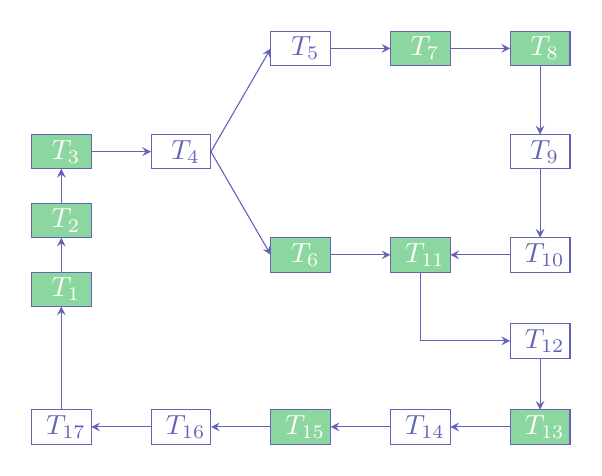
\begin{tikzpicture}[scale=0.38,yscale=1.15]
				%\draw (1,1) grid (19,13);
				\draw[hoccungpi](1,1) rectangle (3,2);
				\draw[hoccungpi](2,1.5) node[] {{ $T_{17}$}};
				\fill[diendantoanhoc!60] (1,5) rectangle (3,6);
				\draw[hoccungpi] (1,5) rectangle (3,6);
				\draw[hoccungpi](2,5.5) node[white] {{ $T_{1}$}};
				\fill[diendantoanhoc!60](1,7) rectangle (3,8);
				\draw[hoccungpi](1,7) rectangle (3,8);
				\draw[hoccungpi](2,7.5) node[white] {{ $T_{2}$}};
				\fill[diendantoanhoc!60] (1,9) rectangle (3,10);
				\draw[hoccungpi] (1,9) rectangle (3,10);
				\draw[hoccungpi] (1,9) rectangle (3,10);
				\draw[hoccungpi](2,9.5) node[white] {{ $T_{3}$}};
				\draw[hoccungpi](5,9) rectangle (7,10);
				\draw[hoccungpi](6,9.5) node[] {{ $T_{4}$}};
				\draw[hoccungpi](5,1) rectangle (7,2);
				\draw[hoccungpi](6,1.5) node[] {{ $T_{16}$}};
				\fill[diendantoanhoc!60](9,1) rectangle (11,2);
				\draw[hoccungpi](9,1) rectangle (11,2);
				\draw[hoccungpi](10,1.5) node[white] {{ $T_{15}$}};
				\fill[diendantoanhoc!60] (9,6) rectangle (11,7);
				\draw[hoccungpi] (9,6) rectangle (11,7);
				\draw[hoccungpi](10,6.5) node[white] {{ $T_{6}$}};
				\draw[hoccungpi](9,12) rectangle (11,13);
				\draw[hoccungpi](10,12.5) node[] {{ $T_{5}$}};
				\draw[hoccungpi](13,1) rectangle (15,2);
				\draw[hoccungpi](14,1.5) node[] {{ $T_{14}$}};
				\draw[hoccungpi] (13,6) rectangle (15,7);
				\fill[diendantoanhoc!60] (13,6) rectangle (15,7);
				\draw[hoccungpi] (13,6) rectangle (15,7);
				\draw[hoccungpi](14,6.5) node[white] {{ $T_{11}$}};
				\fill[diendantoanhoc!60] (13,12) rectangle (15,13);
				\draw[hoccungpi] (13,12) rectangle (15,13);
				\draw[hoccungpi](14,12.5) node[white] {{ $T_{7}$}};
				\fill[diendantoanhoc!60] (17,12) rectangle (19,13);
				\draw[hoccungpi] (17,12) rectangle (19,13);
				\draw[hoccungpi](18,12.5) node[white] {{ $T_{8}$}};
				\draw[hoccungpi](17,9) rectangle (19,10);
				\draw[hoccungpi](18,9.5) node[] {{ $T_{9}$}};
				\draw[hoccungpi](17,6) rectangle (19,7);
				\draw[hoccungpi](18,6.5) node[] {{ $T_{10}$}};
				\draw[hoccungpi](17,3.5) rectangle (19,4.5);
				\draw[hoccungpi](18,4) node[] {{ $T_{12}$}};
				\fill[diendantoanhoc!60] (17,1) rectangle (19,2);
				\draw[hoccungpi] (17,1) rectangle (19,2);
				\draw[hoccungpi](18,1.5) node[white] {{ $T_{13}$}};
				\draw[hoccungpi,-stealth] (2,2) -- (2,5);
				\draw[hoccungpi,-stealth] (2,6) -- (2,7);
				\draw[hoccungpi,-stealth] (2,8) -- (2,9);
				\draw[hoccungpi,-stealth] (3,9.5) -- (5,9.5);
				\draw[hoccungpi,-stealth] (7,9.5) -- (9,12.5);
				\draw[hoccungpi,-stealth] (7,9.5) -- (9,6.5);
				\draw[hoccungpi,-stealth] (11,12.5) -- (13,12.5);
				\draw[hoccungpi,-stealth] (11,6.5) -- (13,6.5);
				\draw[hoccungpi,-stealth] (15,12.5) -- (17,12.5);
				\draw[hoccungpi,-stealth] (18,12) -- (18,10);
				\draw[hoccungpi,-stealth] (18,9) -- (18,7);
				\draw[hoccungpi,-stealth] (17,6.5) -- (15,6.5);
				\draw[hoccungpi,-stealth] (14,6) --(14,4)-- (17,4);
				\draw[hoccungpi,-stealth] (18,3.5) -- (18,2);
				\draw[hoccungpi,-stealth] (17,1.5) -- (15,1.5);
				\draw[hoccungpi,-stealth] (13,1.5) -- (11,1.5);
				\draw[hoccungpi,-stealth] (9,1.5) -- (7,1.5);
				\draw[hoccungpi,-stealth] (5,1.5) -- (3,1.5);
			\end{tikzpicture}
			\caption{\small\textit{\color{hoccungpi}(Các mệnh đề $T_i$ được tô màu xanh là các bất đẳng thức cổ điển, thường được sử dụng.)}}
			\vspace*{-10pt}
		\end{figure}
		Bạn đọc có thể thử sức mình bằng cách tự chứng minh các mũi tên $(T_i)\Rightarrow (T_{j})$ trong sơ đồ trên hoặc tham khảo bài viết [$2$]. (Bạn đọc sẽ tìm thấy trong tài liệu đã dẫn một mạch dài hơn của các bất đẳng thức tương đương với bất đẳng thức Bernoulli). Dưới đây, để minh họa, người viết chỉ điểm qua chứng minh mũi tên $(T_{17}) \Rightarrow (T_{1}).$  Xét số nguyên dương $n$ và số thực $x>0$. Ta có:
		\begin{align*}
			&\dfrac{{{x^{n + 1}} - 1}}{{n + 1}} - \dfrac{{{x^n} - 1}}{n} \\
			= &\dfrac{{x - 1}}{{n(n + 1)}}\left( {n{x^n} - {x^{n - 1}} - {x^{n - 2}} -  \ldots  - 1} \right)\\
			= &\dfrac{{{{(x - 1)}^2}}}{{n(n + 1)}}\left[ {x^{n - 1}} + \left( {{x^{n - 1}} + {x^{n - 2}}} \right) +  \ldots \right. \\
			& \left.+ \left( {{x^{n - 1}} + {x^{n - 2}} +  \ldots  + 1} \right) \right].
		\end{align*}
		Hệ thức trên đây, kết hợp với lập luận bằng quy nạp, dẫn đến
		\begin{align*}
			\frac{{{x^m} - 1}}{m} \geq \frac{{{x^n} - 1}}{n},
		\end{align*}
		với mọi số nguyên dương $m \geq n$. Thay $x^n$ bằng $x$ và $r= \frac{n}{m}$ vào bất đẳng thức vừa thu được, ta có
		\begin{align*}
			{x^r} - 1 \geq  r\left( {x - 1} \right).
		\end{align*}
		Bất đẳng thứuc này đúng với mọi số hữu tỷ $r \geq 1$ và  số thực $x>0$. Lại vì tập các số hữu tỷ
		lớn hơn hoặc bằng $1$ trù mật trong tập các số thực lớn hơn hoặc bằng $1$ nên ta có thể kết luận rằng
		\begin{align*}
			{x^{\alpha} } - 1 \geq  \alpha \left( {x - 1} \right)
		\end{align*}
		với mọi số thực $\alpha \geq 1,x>0$. Thay $x$ bởi $x+1$ ta có bất đẳng thức $(T_1)$. 
		\vskip 0.1cm
		$\pmb{2.}$ \textbf{\color{hoccungpi}Nét đẹp qua phép chứng minh}
		\vskip 0.1cm
		Một lời giải hay, đáng học hỏi chưa hẳn là một lời giải ngắn gọn. Bởi vì điểm hay có thể đến từ ý tưởng hoặc từ kỹ thuật xử lý bài toán (kéo theo là lời giải có thể tương đối dài hoặc không đơn giản). Trong mục này, mời bạn đọc đến với những lời giải như vậy.
		\vskip 0.1cm
		\textbf{\color{hoccungpi}Ví dụ} $\pmb{1.}$
		\textit{Ta nhắc lại hai bất đẳng thức sau:
		\vskip 0.1cm
		$\bullet$ \textbf{\color{hoccungpi}(AM -- GM)} Với mọi số thực dương $a_1, a_2, \ldots, a_n$, ta có
		\begin{align*}
			\dfrac{a_1+a_2+\cdots+a_n}{n} \geq \sqrt[n]{a_1a_2\cdots a_n}.
		\end{align*}
		$\bullet$ \textbf{\color{hoccungpi}(Bất đẳng thức Bernoulli cơ bản)} Với mọi số tự nhiên $n$ và số thực dương $x$, ta có
		\begin{align*}
			x^n \geq 1+n(x-1).
		\end{align*}	
		$a)$ Sử dụng bất đẳng thức AM -- GM, hãy chứng minh bất đẳng thức Bernoulli cơ bản.
		\vskip 0.1cm
		$b)$ Sử dụng bất đẳng thức Bernoulli cơ bản, hãy chứng minh bất đẳng thức AM -- GM.}
		\vskip 0.1cm
		\textit{Lời giải.}
		$a)$ Với $n=0,1$ thì bất đẳng thức Bernoulli cơ bản là hiển nhiên vì nó trở thành đẳng thức. Giả sử $n \geq 2$. Ta xét hai trường hợp 
		\vskip 0.1cm
		$\bullet$ Với $0<x \le 1-\dfrac{1}{n}$ thì bất đẳng thức là hiển nhiên do vế trái dương trong khi vế phải không dương.
		\vskip 0.1cm
		$\bullet$ Với $x>1-\dfrac{1}{n}$, áp dụng bất đẳng thức AM -- GM, ta có
		\begin{align*}
			{x^n}{\rm{ }} &= {\left\{ {\frac{{[1 + n(x - 1)] + \overbrace {1 +  \ldots  + 1}^{n - 1}}}{n}} \right\}^n} \\
			&\ge [1 + n(x - 1)] \cdot 1 \cdot  \ldots  \cdot 1 = 1 \!+\! n(x \!-\! 1).
		\end{align*}
		Ta chứng minh xong bất đẳng thức Bernoulli cơ bản.
		\vskip 0.1cm	
		$b)$ Đặt
		\begin{align*}
			A_n=\dfrac{a_1+a_2+\cdots+a_n}{n},
		\end{align*}
		trong đó $a_1, a_2, \ldots$ là các số thực dương. 
		Trước hết, với $n=1$ thì bất đẳng thức cần chứng minh là tầm thường 
		Xét trường hợp $n \geq 2$. Áp dụng bất đẳng thức Bernoulli, ta có
		\begin{align*}
			\left(\frac{A_{n}}{A_{n-1}}\right)^{n} & \geq 1+n\left(\frac{A_{n}}{A_{n-1}}-1\right) \\
			&=\frac{A_{n-1}+n A_{n}-n A_{n-1}}{A_{n-1}} \\
			&=\frac{n A_{n}-(n-1) A_{n-1}}{A_{n-1}}=\frac{a_{n}}{A_{n-1}}.
		\end{align*}
		Hay nói cách khác,
		\begin{align*}
			A_{n}^{n} \geq a_{n} \cdot A_{n-1}^{n-1}.
		\end{align*}		
		Áp dụng liên tục các bất đẳng thức như vậy, ta thu được
		\begin{align*}
			A_{n}^{n}  &\geq a_{n} \cdot A_{n-1}^{n-1} \geq a_{n} \cdot a_{n-1} \cdot A_{n-2}^{n-2}  \\
			&\geq \cdots \geq a_{n} \cdot a_{n-1} \cdots a_{3} \cdot A_{2}^{2} \\
			&\geq a_{n} \cdot a_{n-1} \cdots a_{3} \cdot a_2 \cdot a_1.
		\end{align*}
		Thế nhưng bất đẳng thức $A_n^n \geq a_1a_2 \cdots a_n$ tương đương với $\dfrac{a_1+a_2+\cdots+a_n}{n} \geq \sqrt[n]{a_1a_2\cdots a_n}$ nên bất đẳng thức AM -- GM được chứng minh.
		\vskip 0.1cm
		\textbf{\color{hoccungpi}Ví dụ} $\pmb{2.}$ \textit{Cho số thực $x>-1$ và số nguyên $k$. Chứng minh rằng $(1+x)^{k} \geq 1+ k x.$}
		\vskip 0.1cm
		 Lưu ý: trong ví dụ trên, số nguyên $k$ có thể âm.
		\vskip 0.1cm
		Với mỗi $x>-1$ cố định, ta xét hàm $\mathscr{B}$  sau đây:
		\begin{align*}
			\mathscr{B}: \mathbb{Z} & \rightarrow \mathbb{R} \\
			k&  \mapsto (1+x)^{-k}(1+k x).
		\end{align*}
		Có thể thấy rằng  $\mathscr{B}(0)= \mathscr{B}(1)=1$. 
		Ta sẽ chứng minh $1$ cũng chính là giá trị lớn nhất của $\mathscr{B}$, từ đó ta thu được kết luận của bài toán. Ta có
		\begin{align*}
			&\mathscr{B}(k)-\mathscr{B}(k-1) \\
			=&\frac{1+k x}{(1+x)^{k}}-\frac{1+(k-1) x}{(1+x)^{k-1}} \\
			=&\frac{1\!+\!k x\!-\![1\!+\!(k\!-\!1) x](1\!+\!x)}{(1\!+\!x)^{k}}=\frac{(1-k) x^{2}}{(1+x)^{k}}.
		\end{align*}
		Vì thế $\mathscr{B}(k)-\mathscr{B}(k-1) \ge 0$ nếu $k\le 0$ và $\mathscr{B}(k)-\mathscr{B}(k-1) \le 0$ nếu $k\ge 2$.
		Ta suy ra giá trị lớn nhất của
		$\mathscr{B}$ là $1$ và do đó chứng minh hoàn tất.
		\vskip 0.1cm
		\textbf{\color{hoccungpi}Ví dụ $\pmb{3.}$ (Bất đẳng thức Bernoulli cho số mũ nằm trong khoảng $\pmb{(0;1)}$).}
		\textit{Cho các số thực $x>-1$ và $0<\alpha <1$. Chứng minh rằng}
			$(1+x)^{\alpha} \le 1+ \alpha x.$
		\vskip 0.1cm
		\textit{Lời giải.} Ta xét tập hợp $T$ sau đây:
		\begin{align*}
			&T=\{\alpha \in (0;1): \forall \,\,y>-1 \\
			&\textrm{ thì } (1+y)^{\alpha} \le 1+ \alpha y\}.
		\end{align*}
		Trước tiên, ta sẽ chứng minh $T$ có ba tính chất sau:
		\vskip 0.1cm
		$(1)$ $\dfrac{1}{2} \in T$.
		\vskip 0.1cm
		$(2)$ Nếu $\alpha \in T$ thì $1-\alpha \in T$.
		\vskip 0.1cm
		$(3)$ Nếu $\alpha, \beta \in T$ thì $\alpha \beta \in T$. Hơn nữa, nếu $\alpha + \beta<1$ thì $\alpha + \beta\in T$.
		\vskip 0.1cm
		Thật vậy,
		\vskip 0.1cm 
		$(1)$ Trước hết ta thấy rằng $\left(1+\frac{y}{2}\right)^{2}=1+y+\frac{y^{2}}{4} \geq 1+y $, cho nên $1+\dfrac{y}{2} \geq  (1+y)^{\frac{1}{2}}$. Hay nói cách khác $\dfrac{1}{2} \in T$.
		\vskip 0.1cm 
		$(2)$ Giả sử $\alpha \in T$. Với mọi $y>-1$ ta có
		\begin{align*}
			\frac{-y}{1+y}=-1+\frac{1}{1+y}>-1.
		\end{align*}
		Từ đó ta được
		\begin{align*}
			(1+y)^{1-\alpha}&=(1+y)\left(1+\frac{-y}{1+y}\right)^{\alpha} \\
			&\le (1+y)\left(1+\frac{-\alpha y}{1+y}\right) \\
			&=1+(1-\alpha) y .
		\end{align*}
		Như vậy $1- \alpha \in  T$.
		\vskip 0.1cm
		$(3)$ Giả sử $\alpha, \beta \in T$ với $0<\alpha < \beta <1$. Khi~đó:
		\begin{align*}
			(1\!\!+\!\!y)^{\alpha  \beta}\!=\!\left[(1\!\!+\!\!y)^{\alpha}\right]^{\beta} \!\!\leq\!\! (1\!\!+\!\alpha y)^{\beta} \!\!\le\!\! 1\!\!+\!\alpha  \beta y.
		\end{align*}
		Tức là $\alpha \beta \in T$. Hơn nữa,
		\begin{align*}
			&(1+y)^{\alpha+\beta} \\
			=&(1+y)^{\alpha}(1+y)^{\beta} \leq (1+\alpha y)(1+\beta y) \\
			=&1+(\alpha+\beta) y+(\alpha  \beta) y^{2} \\
			=&\left(\!1\!+\!\frac{\alpha+\beta}{2} y\right)^{2}\!+\!\left[\alpha  \beta\!-\!\left(\frac{\alpha\!+\!\beta}{2}\right)^{2}\right] y^{2} \\
			\leq&\left(\!1+\frac{\alpha+\beta}{2} y\right)^{2}.
		\end{align*}
		Tức là
		\begin{align*}
			(1+y)^{\frac{\alpha+\beta}{2}} \leq 1+\frac{\alpha+\beta}{2} y.
		\end{align*}
		Như vậy ta được $\dfrac{\alpha +\beta }{2} \in T.$
		\vskip 0.1cm
		Tiếp theo, bằng phương pháp quy nạp theo $n,$ và sử dụng các tính chất $(1)$ và $(3)$, ta chứng minh được rằng: 
		\begin{align*}
			A=\left\{\dfrac{m}{2^n}:m,n \in \mathbb{N}^*,m<2^n\right\} \subseteq T.
		\end{align*}
		Cuối cùng, vì $A$ trù mật trong $(0;1)$ nên $T$ cũng trù mật trong $(0;1)$. Từ đây, bằng cách lập luận dựa vào tính chất liên tục, ta thấy rằng $T=(0,1)$. (Cụ thể, với một dãy số $\alpha_i\in T$ mà $\lim\alpha_i= \alpha$ thì $\alpha \in T$).
		Suy ra với mọi số thực $0<\alpha <1$ và mọi số thực $x>-1$ thì
		\begin{align*}
			(1+x)^{\alpha} \le 1+ \alpha x.
		\end{align*}
			Chứng minh hoàn tất.
		\vskip 0.1cm
		$\pmb{3.}$ \textbf{\color{hoccungpi}Bất đẳng thức Bernoulli qua một số bài toán Olympic}
		\vskip 0.1cm
		Bất đẳng thức Bernoulli khi áp dụng cũng đòi hỏi một số kỹ thuật nhất định. Mời bạn đọc khám phá chúng qua các bài toán sau.
		\vskip 0.1cm
		\textbf{\color{hoccungpi}Bài tập $\pmb{1}$ (Olympic New Zealand  năm $\pmb{2019}$).}
		\textit{Cho $a,b,c$ là các số thực dương có tổng bằng $3$. Chứng minh rằng:}
		\begin{align*}
			a^a + b^b + c^c \ge 3.
		\end{align*}
		\textbf{\color{hoccungpi}Bài tập $\pmb{2.}$ (Olympic Nhật Bản năm $\pmb{2005}$).}
		\textit{Cho $a, b, c$ là các số thực dương có tổng bằng $1$. Chứng minh rằng:}
		\begin{align*}
			a \sqrt[3]{\!1\!+\!b\!-\!c}\!+\!b \sqrt[3]{\!1\!+\!c\!-\!a}\!+\!c \sqrt[3]{\!1\!+\!a\!-\!b} \!\leq\! 1 .
		\end{align*}
		\textbf{\color{hoccungpi}Bài tập $\pmb{3.}$ (Dự tuyển kỳ thi IMO năm $\pmb{2004}$).}
		\textit{Cho $a,b,c$ là các số thực dương thỏa mãn $ab+bc+ca=1$. Chứng minh rằng:}
		\begin{align*}
			\sqrt[3]{\frac{1}{a}+6 b}+\sqrt[3]{\frac{1}{b}+6 c}+\sqrt[3]{\frac{1}{c}+6 a} \leq \frac{1}{a b c}.
		\end{align*}
		\textbf{\color{hoccungpi}Bài tập $\pmb{4.}$ (Olympic Bắc Trung Quốc  năm $\pmb{2009}$).}
		\textit{Cho $x,y,z$ là các số thực dương thỏa mãn $ x^2+y^2+z^2 = 3.$ Chứng minh rằng:}
		\begin{align*}
				&\dfrac{{{x^{2009}} - 2008(x - 1)}}{{y + z}} + \dfrac{{{y^{2009}} - 2008(y - 1)}}{{x + z}} \\
				&+ \dfrac{{{z^{2009}} - 2008(z - 1)}}{{x + y}} \ge \dfrac{1}{2}(x + y + z).
		\end{align*}
		\textbf{\color{hoccungpi}Bài tập $\pmb{5.}$ (Kỳ thi tuyển chọn đội tuyển Đài Loan năm $\pmb{2016}$).}
		\vskip 0.1cm
		\textit{Cho $a,b,c$ là các số thực không âm thỏa mãn:
		\begin{align*}
			(a+b)(b+c)(c+a) \neq 0.
		\end{align*}
		Tìm giá trị nhỏ nhất của biểu thức:}
		\begin{align*}
			P=&{(a + b + c)^{2016}}\left(\frac{1}{{{a^{2016}} + {b^{2016}}}}\right.\\
			 &\left.+ \frac{1}{{{b^{2016}} + {c^{2016}}}} + \frac{1}{{{c^{2016}} + {a^{2016}}}}.\right)
		\end{align*}
		\textbf{\color{hoccungpi}Bài tập $\pmb{6.}$ (Dự tuyển kỳ thi IMO năm $\pmb{2001}$).} \textit{Cho $\{a_n\}$ là một dãy các số thực dương. Chứng minh rằng có vô số $n$ sao cho:}
		\begin{align*}
			1 + a_n > a_{n-1} \sqrt[n]{2}.
		\end{align*}
		\textbf{\color{hoccungpi}Bài tập $\pmb{7.}$ (Dự tuyển kỳ thi IMO năm $\pmb{2017}$).}
		\textit{Cho $a_1,a_2,\cdots,a_n,k,M$ là các số nguyên dương sao cho: 
		\begin{align*}
			\frac{1}{a_1}\!+\!\frac{1}{a_2}\!+\!\cdots\!+\!\frac{1}{a_n}\!=\!k\,\,\text{ và }\,\, a_1a_2\cdots a_n=M.
		\end{align*}
		Chứng minh rằng nếu $M>1$ thì
		$M(x+1)^k <(x+a_1)(x+a_2)\cdots (x+a_n)$ với mọi $ x>0.$}
		\vskip 0.1cm
		\textbf{\color{hoccungpi}Lời kết}
		\vskip 0.1cm
		Việc nhìn lại các bất đẳng thức và tìm ra sợi dây liên kết giữa chúng cũng là một cách học bất đẳng thức  thú vị. Chắc hẳn những sợi dây như vậy sẽ còn rất nhiều, chúng đang chờ bạn đọc khám phá.  Cuối cùng, người viết gửi lời cảm ơn đến tác giả Trần Nam Dũng đã có bài viết gợi mở cho bài viết này, và đến người phản biện vì những góp ý bổ ích cho bài viết.
		\vskip 0.1cm
		\textbf{\color{hoccungpi}Tài liệu tham khảo.}
		\vskip 0.1cm
		[$1$] Trần Nam Dũng, \textit{Bất đẳng thức Bernoulli}. Tạp chí Pi, số $10$ năm $2021$. 
		\vskip 0.1cm
		[$2$] Yuan--Chuan Li, Cheh--Chih Yeh. \textit{Some Equivalent Forms of Bernoulli's Inequality: A Survey}.  Applied Mathematics, $2013$.
		\vskip 0.1cm
		[$3$] Maligranda, L. \textit{The AM--GM Inequality is Equivalent to the Bernoulli Inequality}. Math Intelligencer $34$, $1-2$ ($2012$).
\end{multicols}
%	\newpage
%	
%	\setcounter{figure}{0}
%	\thispagestyle{cackithitoannone}
\pagestyle{cackithitoan}
\everymath{\color{cackithi}}
\graphicspath{{../cackithi/pic/}}
\blfootnote{{\color[named]{cackithi}$^1$Trường Đại học Mỏ--Địa chất.}}
\begingroup
\AddToShipoutPicture*{\put(0,616){\includegraphics[width=19.3cm]{../bannercackithi}}} 
\AddToShipoutPicture*{\put(64,526){\includegraphics[scale=1]{../tieude3.pdf}}}
\centering
\endgroup
\vspace*{180pt}

\begin{multicols}{2}
	Xin được giới thiệu với bạn đọc về kỳ thi ``chinh phục đồi chim sẻ". Đây là kỳ thi do Trường đại học tổng hợp Moscow và nhà xuất bản thanh niên Moscow cùng phối hợp tổ chức từ năm $2005$ nhằm tuyển chọn sinh viên cho trường Đại học tổng hợp Moscow. Xin được nói thêm Trường Đại học tổng hợp Moscow là trường đại học lâu đời nhất và cũng là trường đại học nổi tiếng nhất nước Nga. Nơi đây đã đào tạo ra rất nhiều nhà khoa học danh tiếng. Thi đỗ vào trường là niềm mơ ước của rất nhiều học sinh Nga. Tham gia kỳ thi này là học sinh các lớp từ $9$ tới $11$. Trong đó có kỳ thi riêng dành cho lớp $11$ và cho các bạn lớp $9$ và $10$. Năm $2009$ có $500$ bạn học sinh đã được giải thưởng kỳ thi này và khoảng $400$ bạn đã trở thành sinh viên của trường. Sau đây là bài kiểm tra của năm $2021$.
	\vskip 0.1cm
	Kỳ thi ``Chinh phục đồi chim sẻ" năm học $2020/2021$ gồm hai vòng và đều tiến hành thi online. Vòng tuyển loại (diễn ra vào tháng $11-12$ năm $2020$) kéo dài $24$h gồm hai vòng nhỏ hơn: vòng loại có $6$ bài toán và kéo dài $3$ giờ, phần sáng tạo gồm $3$ bài toán và cần phải gửi lời giải trong khoảng thời gian còn lại. Vượt qua vòng tuyển loại, các bạn trẻ sẽ được tham gia vào vòng chung kết diễn ra vào tháng $4$ năm $2021$.
	\vskip 0.1cm
	\textbf{\color{cackithi}Vòng loại}
	\vskip 0.1cm
	\textit{Mỗi học sinh sẽ nhận được danh sách các bài toán riêng khác biệt. Sau đây là một ví dụ về sáu bài toán của vòng loại.}
	\vskip 0.1cm
	$\pmb{1.}$ Giải bất phương trình
	\begin{align*}
		\dfrac{{\sqrt {x + 5}  - x - 3}}{{{x^2} - 15x + 54}} \ge 0
	\end{align*}
	Trong đó hãy tìm số lượng nghiệm nguyên của bất phương trình trên.
	\vskip 0.1cm
	$\pmb{2.}$ Giải phương trình $\cos 2x + \cos 6x + 2\sin^2 x = 1$.
	\vskip 0.1cm
	Trong đó hãy chỉ ra tổng các nghiệm thuộc đoạn $\left[ {\dfrac{{5\pi }}{6};\;\pi } \right]$, làm tròn tới hai chữ số sau dấu phảy.
	\vskip 0.1cm
	$\pmb{3.}$ Từ điểm $M$ nằm trong tam giác $ABC$ hạ các đường vuông góc xuống các cạnh $BC$, $AC$, $AB$. Các đường vuông góc này có độ dài tương ứng là $k$, $l$ và $m$. Tìm diện tích của tam giác $ABC$, biết rằng $\angle CAB = \alpha$ và  $\angle ABC = \beta$. Nếu kết quả thu được không là số nguyên, hãy làm tròn nó tới số nguyên gần nhất.
	\vskip 0.1cm
	Cho biết các giá trị số là:  $\alpha = \dfrac{\pi}{6}, \beta = \dfrac{\pi}{4},k=3  ,l=2  ,m=4$.
	\vskip 0.1cm 
	$\pmb{4.}$ Giải hệ sau
	\begin{align*}
		\begin{cases}
			x^3 + 3y^2 = 11,\\
			x^2y + xy^2 = 6.
		\end{cases}
	\end{align*}
	Với mỗi nghiệm $(x,y)$ của hệ, hãy tính giá trị của biểu thức $\dfrac{x}{y}$; sau đó tìm giá trị nhỏ nhất trong các giá trị thu được -- lấy xấp xỉ tới hai chữ số sau dấu phảy.
	\vskip 0.1cm
	$\pmb{5.}$ Có hai hợp kim. Hợp kim thứ nhất chứa $p\%$ tạp chất, hợp kim thứ hai chứa $q\%$ hợp chất. Hỏi rằng cần phải nung chảy hai hợp kim theo một tỷ lệ nào để thu được một hợp kim mới chứa $r\%$ tạp chất. Trong đáp án khi tính xấp xỉ tỷ lệ khối lượng của hợp kim thứ nhất với khối lượng của hợp kim thứ hai thì làm tròn tới hai chữ số sau dấu phảy.
	\vskip 0.1cm
	Các dữ liệu số: $p = 70, q = 5, r = 40$.
	\vskip 0.1cm
	$\pmb{6.}$ Hãy tìm tất cả các số nguyên $a$ có giá trị tuyệt đối không vượt quá $15$ sao cho bất đẳng thức 
	\begin{align*}
		\dfrac{{4x - a - 4}}{{6x + a - 12}} \le 0
	\end{align*}
	thỏa mãn với mọi $x$ thuộc khoảng  $[2,3]$. Sau đó hãy tính tổng tất cả các giá trị $a$ vừa tìm được.
	\vskip 0.1cm
	\textbf{\color{cackithi}Vòng tuyển chọn (phần sáng tạo)}
	\vskip 0.1cm
	$\pmb{7.}$ Tìm tất cả các số tự nhiên $n$ không vượt quá $100$ sao cho tổng ${1^2} + {2^2} + {3^2} + ... + {n^2}$  chia hết cho $50$.
	\vskip 0.1cm
	Với những giá trị $n$ vừa tìm được, hãy sắp xếp chúng theo thứ tự tăng dần:  ${n_1} < {n_2} < ... < {n_k}$. Từ đó hãy cho biết $n_{k-2}$ là số nào?
	\vskip 0.1cm
	$\pmb{8.}$ Cho trước một đường tròn, trong tất cả các tam giác nội tiếp đường tròn có tổng bình phương của các góc là $\alpha^2 + \beta^2 = \gamma^2 = \dfrac{\pi^2}{2}$ (các góc  $\alpha$,  $\beta$, $\gamma$ được tính bằng radian) hãy tìm tất cả các tam giác có diện tích lớn nhất.
	\vskip 0.1cm
	Với mỗi tam giác tìm được, hãy tìm giá trị nhỏ nhất của tích các cặp góc. Giá trị nhỏ nhất được làm tròn tới hai chữ số sau dấu phảy. 
	\vskip 0.1cm
	$\pmb{9.}$ Hãy tìm tất cả các cặp số dương $x$, $y$ thỏa mãn đẳng thức
	\begin{align*}
		&\dfrac{{4{x^2}y + 6{x^2} + 2xy - 4x}}{{3x - y - 2}} \\
		&+ \sin \left( {\dfrac{{3{x^2} + xy + x - y - 2}}{{3x - y - 2}}} \right)\\
		= &\,2xy + {y^2} + \dfrac{{{x^2}}}{{{y^2}}} + \dfrac{{2x}}{y} + \dfrac{{2xy({x^2} + {y^2})}}{{{{(3x - y - 2)}^2}}} + \\
		&+ \dfrac{1}{{{{(x + y)}^2}}}\left( {x^2}\sin \dfrac{{{{(x + y)}^2}}}{x}\right. \\
		&\left.+ {y^2}\sin \dfrac{{{{(x + y)}^2}}}{{{y^2}}} + 2xy\sin \dfrac{{{{(x + y)}^2}}}{{3x - y - 2}} \right).
	\end{align*}
	Trong đáp án hãy viết tổng $x^2 + y^2$ của tất cả các nghiệm  $(x,y)$. Kết quả được làm tròn tới hai chữ số sau dấu phảy. 
	\vskip 0.1cm
	\textbf{\color{cackithi}Vòng chung kết}
	\vskip 0.1cm
	\textbf{\color{cackithi}Đề $\pmb{1}$}
	\vskip 0.1cm
	$\pmb{10.}$ Viết các số tự nhiên bắt đầu từ $20$ thành một dòng: $20212223\ldots$ Hỏi rằng trong dãy kỹ tự thu được, chữ số nào đứng ở vị trí $2021$?
	\vskip 0.1cm
	$\pmb{11.}$ Hãy tìm tất cả các giá trị của $a$ sao cho phương trình
	\begin{align*}
		|x| \!-\! \arcsin x \!+\! b \!\cdot\! (\arccos x\, \!+\! |x| \!-\! 1) \!+\! a \!=\! 0
	\end{align*}
	có ít nhât một nghiệm với mọi giá trị của $b$.
	\vskip 0.1cm
	$\pmb{12.}$ Phương trình sau có bao nhiêu nghiệm
	\begin{align*}
		{2^{\lg ({x^2} - 3)}} = \lg {2^{{x^2} - 2}}?
	\end{align*}
	$\pmb{13.}$ Giải hệ sau
	\begin{align*}
		\begin{cases}
			2x - 3y + \dfrac{1}{xy} = 6,\\
			3z - 6x + \dfrac{1}{xz} = 2,\\
			6y - 2z + \dfrac{1}{yz} = 3.
		\end{cases}
	\end{align*}
	$\pmb{14.}$ Gấp một tờ giấy hình vuông có diện tích là $17$ theo đường thẳng đi qua tâm. Sau đó dính các mảnh lại với nhau. Hãy tìm diện tích lớn nhất trong các hình có thể tạo được.
	\vskip 0.1cm
	Trong khuôn khổ có hạn của bài báo, chúng tôi chỉ trình bày lời giải chi tiết đối với một số bài chọn lọc.  
	\vskip 0.1cm 
	\textbf{\color{cackithi}Đáp án và lời giải}
	\vskip 0.1cm
	\textbf{\color{cackithi}Vòng loại}
	\vskip 0.1cm
	$\pmb{1.}$ Đáp án: $7$.
	\vskip 0.1cm
	$\pmb{2.}$ Đáp án: $2{,}88$ (giá trị chính xác: $\dfrac{11\pi}{12}$).
	\vskip 0.1cm
	$\pmb{3.}$ Đáp án: $67$.
	\vskip 0.1cm
	$\pmb{4.}$ Đáp án: $-1{,}31$ (giá trị chính xác:  $-\dfrac{1+ \sqrt{217}}{12}$).
	\vskip 0.1cm
	$\pmb{5.}$ Đáp án: $1{,}17$ (giá trị chính xác:  $\dfrac{7}{6}$).
	\vskip 0.1cm
	$\pmb{6.}$ Đáp án:  $-7$.
	\vskip 0.1cm
	\textbf{\color{cackithi}Vòng tuyển chọn (phần sáng tạo)}
	\vskip 0.1cm
	$\pmb{7.}$ Đáp án: $87$.
	\vskip 0.1cm
	$\pmb{8.}$ Đáp án: $0{,}27$ (giá trị chính xác: $\dfrac{\pi^2}{36}$).
	\vskip 0.1cm
	$\pmb{9.}$ Đáp án: $4{,}33$ ($x = \dfrac{9 + \sqrt{17}}{8}$, $y = \dfrac{1+ \sqrt{17}}{4}$ và  $x^2 + y^2 = \dfrac{85 + 13\sqrt{17}}{32} \approx 4{,}33$).
	\vskip 0.1cm
	\textbf{\color{cackithi}Vòng chung kết}
	\vskip 0.1cm
	\textbf{\color{cackithi}Đề $\pmb{1}$}
	\vskip 0.1cm
	$\pmb{10.}$ Đáp án: $7$.
	\vskip 0.1cm 
	$\pmb{11.}$ Đáp án:  $\dfrac{\pi}{2} -1$.
	\vskip 0.1cm 
	\textit{Lời giải}. Khi  $b = -1$, phương trình có dạng $|x| - \arcsin x - \arccos x - |x| + 1 + a = 0$. Với $x \in [-1;1]$ phương trình tương đương với $1 + a - \dfrac{\pi}{2} = 0$. Như vậy, khi $b = -1$  nghiệm chỉ tồn tại khi $a = \dfrac{\pi}{2} - 1$.
	\vskip 0.1cm
	Mặt khác, khi $a = \dfrac{\pi}{2} -1$ phương trình $|x| - \arcsin x + b \cdot (\arccos x\, + |x| - 1) + \dfrac{\pi }{2} - 1 = 0$ có nghiệm $x =1$ với bất kỳ giá trị nào của $b$.
	\vskip 0.1cm
	\textit{Chú thích.} Các bạn thí sinh có nhiều lời giải không đúng vì dựa trên suy luận sau: câu văn từ điều kiện của bài toán ``với mọi giá trị của $b$ có ít nhất một nghiệm" thì bị hiểu nhầm là ``có cùng một nghiệm với mọi trí trị của $b$" (Đây là một bài toán khác, đơn giản hơn mặc dù đáp áp của nó trùng với đáp án của bài toán đã cho). 
	\vskip 0.1cm
	$\pmb{12.}$ Đáp án: $4$.
	\vskip 0.1cm 
	\textit{Lời giải.} Phương trình được biến đổi về dạng 
	\begin{align*}
		{t^\alpha } = \alpha (t + 1),
	\end{align*}
	với $\alpha  = \lg 2 \in (0,1)$, $t = {x^2} - 3 > 0$.
	\vskip 0.1cm
	Vì vế trái của phương trình $f\left( t \right) = {t^\alpha }$ là hàm lũy thừa với miền xác định $t \ge 0$; và với $\alpha \in  (0,1)$ thì đây là hàm lõm. Trong khi đó vế phải của phương trình $g(t) = \alpha(t+1)$ là hàm tuyến tính với hệ số góc dương nên đồ thị của hai hàm số $f(t)$ và $g(t)$ sẽ cắt nhau tại không quá hai điểm.
	\vskip 0.1cm
	Vì $f\left( 0 \right) = 0 < \alpha  = g\left( 0 \right)$ và  $f\left( 1 \right) = 1 = \lg 10 > \lg 4 = 2\alpha  = g\left( 1 \right)$, nên trong khoảng $(0;1)$ tồn tại ít nhất một điểm.
	\vskip 0.1cm
	Vì $f(1) > g(1)$, $f\left( {10} \right) = {10^{\lg 2}} = 2 = \lg 100 < \lg {2^{11}} = 11\alpha  = g\left( {10} \right)$, nên trong khoảng $(1;10)$ cũng tồn tại ít nhất một nghiệm.
	\vskip 0.1cm
	Điều đó có nghĩa là đồ thị hai hàm số cắt nhau tại đúng hai điểm (một điểm nằm giữa $0$ và $1$, một điểm khác nằm giữa $1$ và $10$).
	\vskip 0.1cm 
	Mỗi nghiệm dương $t$ lại sinh ra hai nghiệm $х$ của phương trình đầu. Vì vậy, có cả thảy là $4$ nghiệm.
	\vskip 0.1cm
	$\pmb{13.}$ Đáp án:  $x = \dfrac{1}{2}, y = \dfrac{1}{3}, z= 1$  và  $x = -\dfrac{1}{2}, y = - \dfrac{1}{3}  , z= -1$.
	\vskip 0.1cm 
	\textit{Lời giải.} Nhân phương trình đầu với  $(2x - 3y)$, phương trình hai với $(3z-6x)$, phương trình thứ ba với $(6y-2z)$. Sau đó cộng chúng lại và thu được phương trình hệ quả:
	\begin{align*}
		&{\left( {2x - 3y} \right)^2} + {\left( {3z - 6x} \right)^2} + {\left( {6y - 2z} \right)^2} \\
		&+ \dfrac{{2x - 3y}}{{xy}} + \dfrac{{3z - 6x}}{{xz}} + \dfrac{{6y - 2z}}{{yz}}\\
		&= 6\left( {2x \!-\! 3y} \right) \!+\! 2\left( {3z \!-\! 6x} \right) \!+\! 3\left( {6y \!-\! 2z} \right)\\
		\Leftrightarrow &\,\,{\left( {2x \!-\! 3y} \right)^2} \!+\! {\left( {3z \!-\! 6x} \right)^2} \!+\! {\left( {6y \!-\! 2z} \right)^2} \!=\! 0\\
		\Leftrightarrow &\,\,2x = 3y = z
	\end{align*}
	Thế $2x = 3y = z$ vào hệ, ta được:  $x = \dfrac{1}{2}$, $y = \dfrac{1}{3}$, $z =1$ hoặc $x = - \dfrac{1}{2}$, $y = - \dfrac{1}{3}$,  $z = -1$.
	\vskip 0.1cm 
	Chú thích. Dễ dàng nhận thấy là nếu  $2x = 3y = z$, thì tất cả các nhân tử nhân thêm vào phương trình đều bằng $0$. Thế nhưng nó không làm xuất hiện nghiệm ngoại lai vì phương trình tổng vẫn là phương trình hệ quả của hệ đã cho.
	\vskip 0.1cm
	$\pmb{14.}$ Đáp án:  $17\left( {2 - \sqrt 2 } \right)$.
	\vskip 0.1cm 
	\textit{Lời giải.} Gọi cạnh của hình vuông là $a$. Giả sử đường thẳng cắt và tạo trên cạnh hình vuông $AD$ một đoạn $AP = x < \dfrac{a}{2}$  (Hình $2$).
	\begin{figure}[H]
		\vspace*{-5pt}
		\centering
		\captionsetup{labelformat= empty, justification=centering}
		\includegraphics[width= 1\linewidth]{1a.pdf}
		\caption{\small\textit{\color{cackithi}Hình $2$}}
		\vspace*{-10pt}
	\end{figure}
	Hình vẽ thu được đối xứng qua đường thẳng $PR$. Mặt khác, hình vuông $A_1B_1C-1D_1$ là ảnh của hình vuông $ABCD$ qua phép quay quanh tâm của hình vuông. Khi đó  $x = AP = P{A_1} = {C_1}R = RC = BM = M{D_1}$. Vì vậy các tam giác vuông  $AQP$,  $MBN$,  $NC_1R$, $QD_1M$ là bằng nhau. 
	\vskip 0.1cm
	Như vậy diện tích của hình thu được bằng tổng diện tích của hình thang vuông $PD_1C_1R$ và diện tích của hai tam giác vuông bằng nhau  $AQP$,  $MBN$. Diện tích hình thang vuông bằng  $\dfrac{a^2}{2}$. Vì vậy ta cần tìm diện tích lớn nhất của tam giác vuông $AQP$. Chu vi của nó là $AP + AQ + QP = BM + AQ + QM = AB = a$. Trong số các tam giác vuông có chu vi không đổi, thì tam giác vuông cân có diện tích lớn nhất.
	\vskip 0.1cm
	Ta sẽ chứng minh khẳng định trên. Gọi $a$, $b$ là các cạnh của tam giác vuông còn $c$ là độ dài của cạnh huyền. Chu vi tam giác là $P = a + b + c$. Sử dụng bất đẳng thức Cauchy có $P = a + b + \sqrt {{a^2} + {b^2}}  \ge 2\sqrt {ab}  + \sqrt {2ab}  = \sqrt {ab} \left( {2 + \sqrt 2 } \right)$. Từ đó suy ra $S = \dfrac{{ab}}{2} \le \dfrac{1}{2}{\left( {\dfrac{P}{{2 + \sqrt 2 }}} \right)^2}$. Đẳng thức xảy ra khi và chỉ khi $a = b$.
	\vskip 0.1cm 
	Ta cũng có thể chứng minh khẳng định trên thuần túy bằng hình học: nếu trong góc vuông $ABC$ dựng một đường tròn nội tiếp có bán kính là $\dfrac{P}{2}$, thì đường tròn này sẽ là đường tròn bàng tiếp của tất cả các tam giác vuông có chu vi là $P$ và các cạnh góc vuông $BX$, $BY$ nằm trên hai cạnh của góc. Vì chu vi cho trước, cho nên tam giác có diện tích lớn nhất là tam giác có bán kính đường tròn nội tiếp lớn nhất. Bán kính này đạt giá trị lớn nhất khi đường tròn nội tiếp tiếp xúc với đường tròn bang tiếp (nếu bán kính lớn hơn nữa thì hai đường tròn này sẽ cắt nhau, đó là điều không thể), tức là khi tam giác cân. 
	Như vậy  $\angle QPA = 45^\circ$, $\angle RPD = \angle QPR = \dfrac{180^\circ - 45^\circ}{2} = 67,5^\circ$. Khi đó $a = AB = 2x + x\sqrt 2 $. Từ đây rút ra được $x = \dfrac{a}{{2 + \sqrt 2 }} = \dfrac{{a\left( {2 - \sqrt 2 } \right)}}{2}$, diện tích tam giác $\Delta QPA$  bằng $\dfrac{{{x^2}}}{2} = \dfrac{{{a^2}\left( {4 + 2 - 4\sqrt 2 } \right)}}{8} = \dfrac{{{a^2}\left( {3 - 2\sqrt 2 } \right)}}{4}$. Điều đó có nghĩa là diện tích cần tìm là $\dfrac{{{a^2}}}{2} + 2 \cdot \dfrac{{{a^2}\left( {3 - 2\sqrt 2 } \right)}}{4} = \dfrac{{{a^2}\left( {1 + 3 - 2\sqrt 2 } \right)}}{2} = {a^2}\left( {2 - \sqrt 2 } \right)$.
	\vskip 0.1cm 
	Vẫn tồn tại một lời giải khác hoàn toàn bằng đại số. Giả sử cạnh của hình vuông bằng $a$, đường thẳng cắt cạnh $AD$ của hình vuông một đoạn  $AP = x < \dfrac{a}{2}$. Ta sẽ đi tìm $AQ$. Ký hiệu các góc $\angle RPS = \angle RPQ = \alpha $, $\angle QPA = \beta$. Từ tam giác $PRS$ (với $S$ là hình chiếu của điểm $R$ lên cạnh $AD$), ta tìm được ${\rm{tg}}\,\alpha  = \dfrac{a}{{a - 2x}}$. Do đó  ${\rm{tg}}\,(2\alpha ) = \dfrac{{a(a - 2x)}}{{2x(x - a)}}$,  $AQ = x \cdot {\rm{tg}}\,\beta  = x{\rm{tg}}\,( - 2\alpha ) = \dfrac{{a(a - 2x)}}{{2(a - x)}}$.
	\vskip 0.1cm
	Từ đó suy ra, các cạnh của tam giác vuông bằng $x$ và  $\dfrac{{a(a - 2x)}}{{2(a - x)}}$. Khi đó diện tích cần tìm bằng $\dfrac{{{a^2}}}{2} + \dfrac{{ax(a - 2x)}}{{2(a - x)}}$. Bằng cách tính đạo hàm, ta có thể suy ra rằng hàm số $f(x) = \dfrac{{x(a - 2x)}}{{(a - x)}}$  đạt cực đại tại  $x = \dfrac{{a(2 - \sqrt 2 )}}{2}$. Nó tương ứng với các góc  $\beta = \dfrac{\pi}{4}, 2\alpha = \dfrac{3\pi}{4}, \alpha = \dfrac{3\pi}{8}$.
	\vskip 0.1cm
	\textbf{\color{cackithi}Tài liệu tham khảo}
	\vskip 0.1cm
	[$1$] Олимпиада по математике «Покори Воробьевы горы!» -- $2019-2020$ / \textit{Б. А. Будак и др.} // Математика в школе. -- $2021$. -- № 1. С. $28 - 39$.
	\vskip 0.1cm
	[$2$] Олимпиада по математике «Покори Воробьевы горы!» -- $2018-2019$ / \textit{Б. А. Будак и др.} // Математика в школе. -- $2020$. -- № $4$. С. $11 - 23$.
	\vskip 0.1cm
	[$3$] Олимпиада по математике «Покори Воробьевы горы!» -- $2017-2018$ / \textit{Б. А. Будак и др.} // Математика в школе. -- $2018$. -- № $5$. С. $20 - 32$.
	\vskip 0.1cm
	[$4$] Олимпиада по математике «Покори Воробьёвы горы!» -- $2016-2017$ / \textit{Д. В. Горяшин и др.} // Математика в школе. -- $2017$. -- № 8. $С$. $31- 40$.
	\vskip 0.1cm
	[$5$] Олимпиада «Покори Воробьёвы горы!» / \textit{В. В. Галатенко и др.} // Математика в школе. -- $2017$. -- № $2$. С. $12 - 23$.
	\vskip 0.1cm
	[$6$] Олимпиада «Покори Воробьёвы горы!» / \textit{А. С. Зеленский и др.} // Математика в школе. -- $2016$. -- № $4$. С. $10 - 25$.
	\vskip 0.1cm
	[$7$] Олимпиада «Покори Воробьёвы горы!» по математике ($2013 - 2018$) / \textit{А. С. Зеленский и др.} -- М.: МЦНМО, $2019$. -- $192$ С. 
\end{multicols}

%\begin{center}
%	\begin{tikzpicture}[cackithi]
%		\draw  (0.,0.)-- (4.,0.);
%		\draw  (4.,0.)-- (4.,4.);
%		\draw  (4.,4.)-- (0.,4.);
%		\draw  (-0.66,2.98)-- (2.94,4.68);
%		\draw  (2.94,4.68)-- (4.64,1.04);
%		\draw  (4.64,1.04)-- (1.04,-0.66);
%		\draw  (1.04,-0.66)-- (-0.66,2.98);
%		\draw  (0.4947469396520865,-0.3892905719808155)-- (3.638568258286205,4.60090199727969);
%		\draw  (0.,4.)-- (0.,0.);
%
%			\draw [fill=white] (0.,0.) circle (1.6pt);
%			\draw (-0.16,-0.19) node {$A$};
%			\draw [fill=white] (4.,0.) circle (1.6pt);
%			\draw (4.22,-0.25) node {$D$};
%			\draw [fill=white] (4.,4.) circle (1.6pt);
%			\draw (4.3,4.23) node {$C$};
%			\draw [fill=white] (0.,4.) circle (1.6pt);
%			\draw (-0.04,4.53) node {$B$};
%			\draw [fill=white] (2.,2.) circle (1.6pt);
%			\draw (0.46,-0.11) node {$x$};
%			\draw (3.74,2.01) node {$a$};
%			\draw (3.66,4.37) node {$x$};
%			\draw [fill=white] (-0.66,2.98) circle (1.6pt);
%			\draw (-0.67,3.58) node {$D_1$};
%			\draw [fill=white] (2.94,4.68) circle (1.6pt);
%			\draw (3.13,5.1) node {$C_1$};
%			\draw [fill=white] (4.64,1.04) circle (1.6pt);
%			\draw (4.83,1.46) node {$B_1$};
%			\draw [fill=white] (1.04,-0.66) circle (1.6pt);
%			\draw (1.33,-0.7) node {$A_1$};
%			\draw [fill=white] (0.74,0.) circle (1.6pt);
%			\draw (1.02,-0.09) node {$P$};
%			\draw [fill=white] (3.26,4.) circle (1.6pt);
%			\draw (3.2,3.57) node {$R$};
%			\draw (-0.22,3.77) node {$x$};
%			\draw [fill=white] (0.,3.2916666666666674) circle (1.6pt);
%			\draw (0.22,3.13) node {$M$};
%			\draw [fill=white] (0.,1.566823529411764) circle (1.6pt);
%			\draw (0.32,1.73) node {$Q$};
%			\draw [fill=white] (1.5,4.) circle (1.6pt);
%			\draw (1.5,4.45) node {$N$};
%			\draw [decorate, decoration = {mirror,brace,raise=5pt}] (-0.66,2.98) --  (0.74,0.);
%			\draw (-0.5,1.65) node[left] {$a-x$};
%	\end{tikzpicture}
%\end{center}
%	\newpage
%	
%	\setcounter{figure}{0}
%	\thispagestyle{diendandayvahoctoannone}
\pagestyle{diendandayvahoctoan}
\everymath{\color{diendantoanhoc}}
\graphicspath{{../diendantoanhoc/pic/}}
%\blfootnote{$^{1}$\color[named]{diendantoanhoc}...}
\begingroup
\AddToShipoutPicture*{\put(0,616){\includegraphics[width=19.3cm]{../bannerdiendan}}}
\AddToShipoutPicture*{\put(84,525){\includegraphics[scale=1]{../tieude.pdf}}}
\centering
\endgroup
\vspace*{180pt}

\begin{multicols}{2}
	Trong bài viết này, tôi muốn nhấn mạnh việc giảng dạy Tin học và Công nghệ Thông tin (CNTT) hiện nay còn lạc hậu và điều này hạn chế việc phát triển ngành CNTT của nước ta.  
	\vskip 0.05cm
	$\pmb{1.}$ \textbf{\color{diendantoanhoc}Sự cần thiết của tư duy Tin học}
	\vskip 0.05cm
	Trong một nền kinh tế dựa vào công nghệ cao -- khi mà ``nội dung" sẽ là một trong những mặt hàng chính thì Lập trình -- thao tác trên các dữ liệu thô, tạo ra các tri thức có giá trị trở thành một kỹ năng có nhu cầu cao, một nghề nghiệp thu hút trong thị trường lao động. Gần như mọi khía cạnh của nền kinh tế, mọi hoạt động khoa học ngày nay đều có sự hiện diện của Tin học. Chẳng hạn, ngày nay chúng ta đang ``bơi trong biển dữ liệu", làm thế nào để có thể ``chắt lọc" được từ đó những tri thức đáng giá -- ``xử lý dữ liệu lớn" là minh chứng rõ nét cho nhu cầu này.
	\vskip 0.05cm
	Chính vì thế, có được một tư duy tốt về thuật toán và kỹ năng lập trình sẽ giúp ích rất lớn cho học sinh muốn tham gia vào các lĩnh vực khoa học -- công nghệ.
	\vskip 0.05cm
	Có thể nói, Tin học rèn dũa cho học sinh tư duy thuật toán và tính thực tế. Ở mức độ đơn giản, học sinh có được \textit{kỹ năng giải quyết vấn đề}: từ một tập hợp đầu vào, cần phải xử lý như thế nào để có được một kết quả thỏa mãn. Ở mức cao hơn, học sinh được rèn luyện \textit{kỹ năng sáng tạo ra vấn đề}, rồi tìm cách giải quyết nó. Ngoài ra, Tin học sẽ giúp học sinh có được \textit{sản phẩm} thông qua quá trình lao động. Điều này khiến cho việc học nói chung không chỉ mang tính lý thuyết, mà còn tăng tính thực hành.
	\vskip 0.05cm
	Qua quá trình giảng dạy, tôi nhận thấy việc dạy các kỹ năng lập trình cơ bản sẽ giúp học sinh:
	\vskip 0.05cm
	$\circ$	Tăng tốc quá trình phát triển;
	\vskip 0.05cm
	$\circ$	Thúc đẩy sáng tạo;
	\vskip 0.05cm
	$\circ$	Tăng tính tự tin;
	\vskip 0.05cm
	$\circ$	Năng cao kỹ năng giải quyết vấn đề và tư duy phản biện;
	\vskip 0.05cm
	$\circ$	Thấy được ứng dụng cụ thể của các môn khoa học khác, đặc biệt là Toán học
	\vskip 0.05cm
	$\circ$	Định hướng nghề nghiệp.
	\vskip 0.05cm
	Ở Hoa Kỳ, Cựu Tổng thống Barack Obama trong thông điệp liên bang $2013$, đã nhấn mạnh vào ``việc xây dựng các kỹ năng cho học sinh đáp ứng một nền kinh tế công nghệ cao", và sau này, ông kêu gọi giới trẻ ``thay vì chỉ biết tiêu thụ, hãy sản xuất ra thông tin", và ``không chỉ sử dụng máy điện thoại di động, hãy lập trình cho nó". Hoa Kỳ đã có nhiều chương trình tài trợ đưa việc giảng dạy lập trình vào khối tiểu học và trung học.
	\vskip 0.05cm
	Anh Quốc là quốc gia đầu tiên trên thế giới đã đưa việc học lập trình thành điều bắt buộc trong các trường tiểu học và trung học. Trẻ em sẽ học lập trình ở độ tuổi $5$ đến $16$. Ở giai đoạn $1$, học sinh học viết chương trình nhỏ, các khía cạnh đơn giản của thuật toán, cài đặt và thực thi trên thiết bị điện tử. Trong giai đoạn $2$, học sinh được học cách thiết kế và viết các chương trình phức tạp hơn, tương tác với môi trường xung quanh. Ở giai đoạn $3$ (cấp trung học), học sinh học về đại số Boolean, tư duy thuật toán. Giai đoạn $4$ tập trung vào sáng tạo và định hướng nghề nghiệp.
	\vskip 0.05cm
	$\pmb{2.}$ \textbf{\color{diendantoanhoc}Học Tin học quá muộn sẽ làm ngành CNTT tụt hậu}
	\vskip 0.05cm
	Ở Việt Nam, CNTT là một ngành quan trọng, được Đảng và Nhà nước coi là một mũi nhọn trong việc phát triển kinh tế. Và để có thể cạnh tranh trong ngành công nghiệp, chúng ta cần thật nhiều những chuyên gia -- lập trình, thiết kế hệ thống, quản trị hệ thống. Những người này phải có khả năng tương tác, nhận và bàn giao công việc với các đối tác nước ngoài. Ngành CNTT của chúng ta thực sự thiếu trầm trọng những nhân lực có chất lượng cao.
	\vskip 0.05cm
	Ở Khoa CNTT thuộc Đại học Công nghệ, ĐHQGHN, một trong những điều chúng tôi cố gắng làm, là đưa việc giảng dạy chuyên môn vào ngay từ đầu, nhưng phải đến sau năm thứ ba và thứ tư, sinh viên mới dần có đủ kỹ năng căn bản để đi thực tập. Mặc dù cấp THPT đã có môn lập trình, nhưng gần như sinh viên lên Đại học lại học lại từ đầu.
	\vskip 0.05cm
	Một lý do có lẽ là, hiện nay, Tin học ở cấp THPT là môn phụ, không có mặt trong các kỳ thi quan trọng như Kỳ thi tốt nghiệp THPT hay thậm chí trong cả các kỳ thì tuyển vào ngành CNTT ở các trường đại học. Chính vì thế, nên ở cấp THPT, việc dạy và học Tin học có phần bị buông lỏng. Học sinh không học đủ, không làm được những bài tập lập trình rất cơ bản. Giáo viên Tin học có thể phải kiêm nhiệm thêm hàng núi các công việc ``vô danh" khác và ít có điều kiện trau dồi chuyên môn. Phụ huynh nói chung cũng không quan tâm cho con con em mình học Tin học sớm.
	\vskip 0.05cm
	Trong bất kỳ lĩnh vực nào, để trở thành chuyên gia xuất sắc, bạn phải bỏ ra $10{.}000$ giờ luyện tập. Ngành CNTT cũng không ngoại lệ. Trong lĩnh vực CNTT, rất nhiều hãng khởi nghiệp bởi những thanh niên còn rất trẻ. Và những người rất trẻ này thường được tiếp xúc với máy tính, lập trình từ bé. Nhưng thực tế ở ngay Đại học Công nghệ cho thấy, chỉ có khoảng $1/10$ số sinh viên vào thẳng của Khoa CNTT, Đại học Công nghệ là có nền tảng lập trình tốt (phần lớn là học sinh đạt giải trong kỳ thi HSG Quốc gia môn Tin học). Đa phần trong số $9/10$ sinh viên còn lại dù thi Đại học ở khối A và A$1$ nhưng gần như không biết gì về lập trình, và phải học từ đầu. 
	\vskip 0.05cm
	\textbf{\color{diendantoanhoc}Lời kết}
	\vskip 0.05cm
	CNTT là ngành phụ thuộc rất lớn vào trí tuệ và kỹ năng lao động (kỹ năng lập trình, kỹ năng vận hành các hệ thống tin học). Như vậy ngành CNTT của Việt Nam hoàn toàn có thể ``cất cánh" trở thành một ngành mũi nhọn. Và để tiềm năng này trở thành hiện thực, hãy coi trọng và khích lệ học sinh học Tin học từ bé.
	\vskip 0.05cm
	Việc dạy tin học và lập trình sớm rất cần cho cho toàn bộ học sinh phổ thông, vì ngoài những người sẽ làm nghề lập trình, hầu hết người lao động ở mọi ngành nghề sẽ cần dùng tin học như một công cụ lao động cơ~bản. 
	\vskip 0.05cm
	Hệ thống Giáo dục phổ thông ngày nay đã quá lạc hậu trong việc giảng dạy CNTT. Và tôi kỳ vọng vào công cuộc Đổi mới Giáo dục mà Bộ Giáo dục đang tiến hành có thể góp phần thay đổi thực trạng này. Tuy nhiên với cách triển khai của Bộ Giáo dục, tôi có cảm nhận rằng, môn Tin học sẽ vẫn chỉ là một môn phụ. Nên chăng, các gia đình, các bạn học sinh, hãy tự trang bị cho mình công nghệ, tư duy hiện đại, để vững bước vào kỷ nguyên~số.
\end{multicols}
%	\newpage
%	
%	\setcounter{figure}{0}
%	\thispagestyle{lichsutoanhocnone}
\pagestyle{lichsutoanhoc}
\graphicspath{{../lichsutoanhoc/pic/}}
\everymath{\color{lichsutoanhoc}}
\blfootnote{$^1$\color{lichsutoanhoc}Cộng tác viên Viện Toán học.}
\begingroup
\AddToShipoutPicture*{\put(0,616){\includegraphics[width=19.3cm]{../bannerlichsu}}}
\AddToShipoutPicture*{\put(58,466){\includegraphics[scale=1]{../tieude3.pdf}}}
\centering
\endgroup

\vspace*{240pt}

\begin{multicols}{2}
	\textbf{\color{lichsutoanhoc}Học viện Plato}
		\vskip 0.1cm
		Thế kỷ thứ tư TCN đã mở đầu bằng cái chết của Socrates (khoảng $470-399$ TCN), một học giả đã áp dụng phương pháp biện chứng của Zeno và bác bỏ thuyết Pythagoras của Archytas (khoảng $420-347$ TCN). Socrates thừa nhận rằng khi còn trẻ, ông đã bị thu hút bởi những câu hỏi như tại sao tổng $2 + 2$ lại bằng tích $2 \times 2$  nhưng khi nhận ra rằng cả toán học và khoa học đều không thể thỏa mãn mong muốn của ông để  hiểu bản chất của sự vật, ông đã tự nghiên cứu để hiểu những điều bản chất.
		\vskip 0.1cm
		Trong \textit{Phaedo} của Plato, cuộc đối thoại trong đó những giờ cuối cùng của Socrates được mô tả rất đẹp, chúng ta thấy những nghi ngờ siêu hình sâu sắc như thế nào loại trừ mối quan tâm của Socrate về toán học hoặc khoa học tự nhiên:
		\vskip 0.1cm
		\textit{Tôi không thể tự thỏa mãn bản thân rằng, khi một cái được thêm vào một cái, mà phép cộng được thực hiện trở thành hai. 
		\vskip 0.1cm
		Tôi không thể hiểu làm thế nào khi tách khỏi nhau, mỗi trong số chúng là một chứ không phải hai, và bây giờ, khi chúng được kết hợp lại với nhau, chỉ là sự đặt cạnh nhau, là nguyên nhân khiến chúng trở thành hai.}
		\vskip 0.1cm
		Do đó, ảnh hưởng của Socrates trong sự phát triển của toán học là không đáng kể, nếu không nói là tiêu cực. Điều đáng ngạc nhiên là chính học trò và người ngưỡng mộ ông là Plato đã trở thành cảm hứng toán học của thế kỷ thứ tư TCN. 
		\vskip 0.1cm
		Mặc dù bản thân Plato không có đóng góp kết quả toán học nổi bật cụ thể nào, nhưng ông đã là trung tâm của hoạt động toán học thời gian đó, hướng dẫn và truyền cảm hứng cho sự phát triển của toán học. Tại cửa trường học của ông, Học viện (The Academy) ở Athens, được khắc khẩu hiệu ``Ai không biết hình học không vào đây".
		\begin{tBox}
			ΑΓΕΩΜΕΤΡΗΤΟΣ ΜΗΔΕΙΣ ΕΙΣΙΤΩ.
		\end{tBox}
		Sự nhiệt tình của Plato đối với toán học khiến ông được biết đến không phải với tư cách là một nhà toán học, mà là ``người tạo ra các nhà toán học".
			\end{multicols}
	\begin{figure}[H]
	\vspace*{5pt}
	\centering
	\captionsetup{labelformat= empty, justification=centering}
	\includegraphics[width= 1\linewidth]{H7}
	\caption{\small\textit{\color{lichsutoanhoc}Hình $6$: The School of Athens của Rafael tại Vaticant.}}
	\vspace*{-10pt}
\end{figure}
\begin{multicols}{2}
%		\vskip 0.1cm
		Sáu nhà toán học (ngoài Plato và Aristotle) sống giữa năm mất của Socrates ($399$ TCN) và năm mất của Aristotle ($322$ TCN) -- gồm Theodorus xứ Cyrene (thế kỷ V TCN), Theaetetus (khoảng $414-369$ TCN), Eudoxus xứ Cnidus (khoảng $410-347$ TCN), hai anh em Menaechmus ($380-320$ TCN) và Dinostratus ($390-320$  TCN), và Autolycus xứ Pitane ($360-320$ TCN) -- là những nhà toán học đã có liên kết ít nhiều chặt chẽ với Học viện Plato.
		\vskip 0.1cm
		Rõ ràng là việc Plato rất coi trọng toán học không đến từ Socrates. Trên thực tế, các bài giảng trong thời kỳ đầu và tác phẩm Đối thoại (Dialogues) của Plato hiếm khi đề cập đến toán học. Archytas, một người bạn của Plato, là người đã khiến Plato quan tâm đến toán học, khi Ông đến thăm bạn ở Sicily vào năm $388$ TCN. Có lẽ chính khi đó, Plato mới biết đến năm hình đa diện đều, được liên kết với bốn nguyên tố (nước, lửa, không khí và đất) của Empedocles ($490-430$ TCN) trong một sơ đồ vũ trụ đã mê hoặc các nhà nghiên cứu trong nhiều thế kỷ (Hình $7$). 
		\vskip 0.1cm
		Có thể, sự coi trọng của Pythagoras đối với khối $12$ mặt đều đã khiến Plato xem xét nó, khối đa diện đều thứ năm và cuối cùng, như một biểu tượng của vũ trụ. 
		Plato đặt ý tưởng của ông về đa diện đều thành một cuộc đối thoại có tiêu đề \textit{Timaeus}, được đặt tên cho một người đóng vai trò là người đối thoại chính thuộc trường phái Pythagoras. Không biết Timaeus xứ Locri có thực sự tồn tại không, hay Plato đã phát minh ra Timaeus như một nhân vật để thể hiện quan điểm của Pythagoras, khi ấy vẫn còn mạnh mẽ ở khu vực mà ngày nay là nước Ý. 
		\begin{figure}[H]
				\vspace*{-5pt}
				\centering
				\captionsetup{labelformat= empty, justification=centering}
				\begin{tikzpicture}[scale=0.8, lichsutoanhoc, node font=\small]
						\draw  (0.,0.)-- (3.,3.);
						\draw  (3.,3.)-- (0.,6.);
						\draw  (0.,6.)-- (-3.,3.);
						\draw  (-3.,3.)-- (0.,0.);
						\draw [dashed] (0.,0.)-- (0.,6.);
						\draw [dashed] (-3.,3.)-- (3.,3.);
						\draw[color=black] (1.9,1.45) node {\color{lichsutoanhoc}Ẩm};
						\draw[color=black] (1.8,4.91) node {\color{lichsutoanhoc}Nóng};
						\draw[color=black] (-1.75,4.91) node {\color{lichsutoanhoc}Khô};
						\draw[color=black] (-1.95,1.33) node {\color{lichsutoanhoc}Lạnh};
						\draw(0,6) node[above] {Lửa -- Tứ diện đều};
						\draw(0,0) node[below] {Nước -- Khối $20$ mặt đều};
						\draw(3.4,3) node[rotate=-90] {Đất -- Lập phương};
						\draw(-3.2,3) node[rotate=90] {Không Khí -- Bát diện đều};
					\end{tikzpicture}
				\caption{\small\textit{\color{lichsutoanhoc}Hình $7$: Sơ đồ vũ trụ ứng với khối đa diện.}}
				\vspace*{-10pt}
			\end{figure}
		Các khối đa diện đều thường được gọi là ``vật thể vũ trụ" hoặc ``khối đa diện Plato" bởi vì cách mà Plato trong \textit{Timaeus} đã áp dụng chúng vào giải thích các hiện tượng khoa học.
		\vskip 0.1cm
		Mặc dù đối thoại này, có lẽ được viết khi Plato đã gần bảy mươi tuổi, cung cấp bằng chứng xác thực sớm nhất cho sự liên kết của bốn nguyên tố với khối đa diện đều, phần lớn sự tưởng tượng này có thể là do trường phái Pythagoras.
		\vskip 0.1cm
		Proclus (khoảng $410-485$) quy việc xây dựng hình học vũ trụ cho Pythagoras, nhưng có thể bạn của Plato là Theaetetus (khoảng $414-369$ TCN) đã viết về liên kết giữa vũ trụ và khối đa diện đều. 
		\vskip 0.1cm
		Quyển XIII của \textit{Cơ sở} của Euclid nói rằng chỉ có ba trong số năm khối đa diện là do Pythagoras, và nhờ Theaetetus mà khối bát diện và hai mươi mặt đều đã được biết đến.
		\vskip 0.1cm
		Có vẻ như Theaetetus đã thực hiện một trong những nghiên cứu quy mô nhất về năm khối đa diện, và định lý nói rằng có và chỉ có năm khối đa diện đều là thuộc về Theaetetus. Có lẽ ông cũng là tác giả của các tính toán về tỷ lệ các cạnh của khối đa diện đều và bán kính mặt cầu ngoại tiếp. 
		\vskip 0.1cm
		Theaetetus là một thanh niên Athens chết vì bệnh kiết lỵ kết hợp với vết thương trong trận chiến, và cuộc đối thoại của Plato mang tên ông là một sự tưởng nhớ của Plato đối với người bạn của mình.
		\vskip 0.1cm
		Trong cuộc đối thoại, có bối cảnh trước đó khoảng ba mươi năm, Theaetetus thảo luận với Socrates và Theodorus về bản chất của các đại lượng vô ước với nhau (hay các đại lượng không thông ước với nhau). Người ta đã giả định rằng cuộc thảo luận này phần nào có dạng mà chúng ta tìm thấy trong phần mở đầu của Quyển X của \textit{Cơ sở}.
		\vskip 0.1cm
		Ở đây, sự phân biệt không chỉ được thực hiện giữa các đại lượng thông ước và vô ước, mà còn giữa các đại lượng khi độ dài là vô ước với nhau, nhưng có diện tích thông ước với nhau. Như $\sqrt{3}$  và $\sqrt{5}$  không thông ước về độ dài, nhưng thông ước về diện tích, vì các hình vuông của chúng có tỷ lệ là $3/5$.
		\vskip 0.1cm
		Mặt khác, các đại lượng  $\sqrt{1 + \sqrt{3}}$  và $\sqrt{1 + \sqrt{5}}$ là không thông ước cả về độ dài và diện tích.
		\vskip 0.1cm
		Cuộc đối thoại mà Plato sáng tác để tưởng nhớ người bạn Theaeteus của mình chứa thông tin về một nhà toán học khác, Theodorus xứ Cyrene, thầy của Plato và Theaetetus, người mà Plato ngưỡng mộ và là người đã đóng góp vào sự phát triển của lý thuyết về các đại lượng vô ước. 
		\vskip 0.1cm
		Không biết bằng cách nào mà Theodorus đã làm điều này và tại sao ông lại dừng lại ở $\sqrt{17}$ 
		\vskip 0.1cm
		Theodorus là người đầu tiên chứng minh tính vô tỷ của căn bậc hai của các số nguyên không chính phương từ $3$ đến $17$.	 
		\vskip 0.1cm
		Chứng minh, trong mọi trường hợp, được đưa ra bởi Aristotle khi ông xây dựng trục xoắn ốc dọc theo đoạn $\sqrt{2}$. Các tác phẩm lịch sử cổ đại chỉ ra rằng Theodorus đã khám phá ra điều này và sau này nó được đưa vào \textit{Cơ sở}, nhưng các tác phẩm của Theodorus đã bị mất. 
		\begin{figure}[H]
				\vspace*{-5pt}
				\centering
				\captionsetup{labelformat= empty, justification=centering}
				\includegraphics[width= 0.85\linewidth]{H8}
				\caption{\small\textit{\color{lichsutoanhoc}Hình $8$: Xoắn ốc Theodorus.}}
				\vspace*{-10pt}
			\end{figure}
		Plato có vai trò quan trọng trong lịch sử toán học phần lớn vì ông là người truyền cảm hứng và là người sáng lập Học viện đào tạo ra nhiều nhà toán học, cũng như do sự nhạy bén của ông về sự phân biệt ở Hy Lạp cổ đại giữa số học (theo nghĩa của lý thuyết về các con số) và kỹ thuật tính toán. 
		\vskip 0.1cm
		Plato cho rằng toán học là cần thiết cho doanh nhân và quân sự, ``phải học nghệ thuật của những con số, nếu không anh ta sẽ không biết cách dàn quân".
		\vskip 0.1cm
		Mặt khác, nhà triết học phải là một nhà số học ``bởi vì anh ta phải nhảy ra khỏi biển của những thay đổi và nắm giữ bản thể đích thực." Hơn nữa, Plato nói trong tác phẩm \textit{Cộng hòa (The Republic)}: ``Số học có tác dụng rất lớn và nâng cao, buộc tâm trí nghĩ về số trừu tượng."
		\vskip 0.1cm 
		Trong số học, Plato đã nhìn thấy một hố ngăn cách lý thuyết và các khía cạnh tính toán, cũng như trong hình học, ông cũng tán thành toán học thuần túy chống lại quan điểm duy vật.  
		\vskip 0.1cm
		Bất kỳ một trong số vô số đường kính của đường tròn là trục đối xứng của hình. Bất cứ điểm nào trên một đường thẳng kéo dài vô hạn có thể được coi là tâm của đối xứng, giống như bất kỳ đường thẳng nào vuông góc với đường thẳng đã cho là trục đối xứng của đường thẳng đã cho. Triết học Plato, với sự áp dụng các ý tưởng của nó, tự nhiên sẽ tìm thấy vai trò của đường thẳng và đường tròn giữa các hình hình học. Tương tự, Plato tôn vinh tam giác.
		\vskip 0.1cm 
		Sự liên kết của bốn khối đa diện đầu tiên với bốn yếu tố phổ quát truyền thống của vũ trụ đã cung cấp cho Plato trong \textit{Timaeus}  một lý thuyết thống nhất tuyệt đẹp về vật chất, theo đó mọi thứ đều được xây dựng bằng các tam giác vuông lý tưởng. Toàn bộ sinh lý học, cũng như khoa học về chất trơ, dựa trên các hình tam giác.
		\vskip 0.1cm
		Pythagoras nổi tiếng là người đã thiết lập toán học như một chủ đề tự do, nhưng Plato đã có ảnh hưởng trong việc làm cho toán học trở thành một phần thiết yếu của chương trình đào tạo.
		\vskip 0.1cm
		Có lẽ bị ảnh hưởng bởi Archytas, Plato đã thêm vào các chủ đề ban đầu trong bộ bốn (quadrivium: Số học, Hình học, Âm nhạc, Thiên văn) một môn học mới: Hình học không gian, vì ông tin rằng hình học không gian đã không được nhấn mạnh đầy đủ. Plato cũng thảo luận về nền tảng của toán học, làm rõ một số định nghĩa và xây dựng lại các giả thiết. Ông nhấn mạnh rằng lý luận được sử dụng trong hình học không đề cập đến những con số hữu hình mô tả chúng, mà là những ý tưởng tuyệt đối mà chúng đại diện. 
		\vskip 0.1cm
		Những người theo thuyết Pythagoras đã định nghĩa điểm là ``sự thống nhất có vị trí," nhưng Plato lại nghĩ về nó như là sự khởi đầu của một đường thẳng.
		\vskip 0.1cm 
		Định nghĩa của một đường là ``chiều dài không có chiều rộng" dường như bắt nguồn từ trường phái Plato.
		\vskip 0.1cm
		Trong số học, Plato không chỉ nhấn mạnh sự phân biệt giữa số lẻ và số chẵn, mà còn là các loại ``chẵn nhân chẵn", ``chẵn nhân lẻ" và ``lẻ nhân lẻ". Mặc dù ta biết rằng Plato đã thêm vào các tiên đề của toán học, chúng ta không có một cơ sở nào để khẳng định điều này.
		\vskip 0.1cm
		Rất ít đóng góp toán học cụ thể được quy cho Plato. Một công thức cho bộ ba Pythagoras -- ${(2n)^2} + {({n^2} - 1)^2} = {({n^2} + 1)^2}$, trong đó  $n$ là số tự nhiên bất kỳ -- mang tên Plato, nhưng đây chỉ là một phiên bản sửa đổi của kết quả được người Babylon và người Pythagoras đã biết. 
		\vskip 0.1cm
		Có lẽ thực sự có ý nghĩa quan trọng hơn cả trong những thứ được gán cho Plato là cái gọi là phương pháp phân tích (analytic method).
		\vskip 0.1cm
		Trong chứng minh toán học, ta bắt đầu với những gì đã cho, và từ các tiên đề và các định đề. Tiến hành từng bước một, sau đó đến khẳng định cần được chứng minh.
		\vskip 0.1cm
		Plato dường như đã chỉ ra rằng  về mặt sư phạm, khi không tìm được một chuỗi lý luận hiển nhiên từ giả thiết đến kết luận, thường là thuận tiện hơn nếu ta bắt đầu bằng mệnh đề cần được chứng minh và từ đó suy ra một kết luận được biết là đúng. Nếu, sau đó, có thể đảo ngược các bước trong chuỗi lý luận này, kết quả sẽ là mệnh đề đã được chứng minh.
		\vskip 0.1cm
		Plato không hẳn là người đầu tiên nêu lên quan điểm phân tích.  Nhưng những gì Plato có thể đã làm là chính thức hóa quá trình này, hoặc có thể ông đã đặt tên cho nó.
		\vskip 0.1cm
		Vai trò của Plato trong lịch sử toán học vẫn còn bị tranh cãi gay gắt. Một số người coi ông là một nhà tư tưởng đặc biệt sâu sắc và nhạy bén. Những người khác hình dung ông như một người đã thu hút các nhà toán học theo con đường lý luận trừu tượng, đi xa những vấn đề thực tiễn. 
		\vskip 0.1cm
		Trong mọi trường hợp, ít ai có thể phủ nhận rằng Plato đã có tác động to lớn đối với sự phát triển của toán học. Học viện Plato ở Athens trở thành trung tâm toán học của thế giới, và từ ngôi trường này, xuất hiện các giáo viên và nghiên cứu viên hàng đầu đến vào giữa thế kỷ thứ tư TCN. Trong số này, nổi tiếng nhất là Eudoxus xứ Cnidus (khoảng $408-335$ TCN),  một học trò của Plato và người đã trở thành nhà toán học và nhà thiên văn học nổi tiếng nhất trong thời đại của mình.
		\vskip 0.1cm
		\textbf{\color{lichsutoanhoc}Tài liệu chính dùng để soạn}
		\vskip 0.1cm
		[$1$] David M. Burton, \textit{The History of Mathematics, An Introduction}, Seventh Edition, McGraw--Hill, $2011$. Chapter $3$: The Beginnings of Greek Mathematics, pp. $116-139$.
		\vskip 0.1cm
		[$2$] Euclid’s \textit{Elements of Geometry}, edited and provided with a modern English translation by Richard Fitzpatrick, Independently published, $2008$, $544$ p.
		\vskip 0.1cm
		[$3$] David Fowler, \textit{The Mathematics of Plato’s Academy}, Second Edition, Clarendon Press, Oxford, $1999$, $441$ p.
		\vskip 0.1cm   
		[$4$] Thomas Heath, \textit{A History of Greek Mathematics}, Oxford at the Clarendon Press, $1921$, Volume $1$: From Thales to Euclid, pp. $170-315$.
		\vskip 0.1cm   
		[$5$] Victor J. Katz, \textit{A History of Mathematics, An Introduction}, Third Edition, Addison--Wesley, $2009$. Chapter $2$: \textit{The Beginnings of Mathematics in Greek}, pp. $40-49$.
		\vskip 0.1cm
		[$6$] Uta C. Merzbach and Carl B. Boyer, \textit{A
			History of Mathematics}, Third Edition, John Wiley \& Sons, $2011$, pp. $65-80$.
		\vskip 0.1cm
		[$7$] George Johston Allman, \textit{Greek Geometry, From Thales to Euclid}, Dublin Universty Press, $1885$, $432$ p.
		\vskip 0.1cm  
		[$8$] R. Lloyd, \textit{Early Greek Science: Thales to Aristotle}, $1970$, Chatto \& Windus, London, $156$ p.
		\vskip 0.1cm 
		[$9$] Arpad Szabo, \textit{The beginnings of Greek Mathematics}, Springer, $1978$, $363$ p.
\end{multicols}
%	\newpage
%
%	 \setcounter{figure}{0}
%	 \thispagestyle{timhieukhoahocnone}
\pagestyle{timhieukhoahoc}
\everymath{\color{timhieukhoahoc}}
\blfootnote{$^1$\text{\color{timhieukhoahoc}Chưa có thống nhất về thuật ngữ tiếng Việt cho ``entanglement". Từ này còn được dịch là ``vướng mắc, ``vướng víu",}}
\blfootnote{\text{\color{timhieukhoahoc}``rối", ``ràng buộc".}}
\blfootnote{$^2$\text{\color{timhieukhoahoc}Nguồn: \url{https://www.nobelprize.org/uploads/2022/10/popular-physicsprize2022.pdf.}}}
\blfootnote{\text{\color{timhieukhoahoc}Dịch: Nguyễn Hoàng Thạch (Viện Toán học); hiệu đính: Nguyễn Trần Thuật (ĐHKHTN -- ĐHQG Hà Nội).}}
\graphicspath{{../timhieukhoahoc/pic/}}
\begingroup
\AddToShipoutPicture*{\put(0,616){\includegraphics[width=19.3cm]{../bannertimhieu}}}
\AddToShipoutPicture*{\put(112,542){\includegraphics[scale=1]{../tieude.pdf}}}
\centering
\endgroup
\vspace*{160pt}

\begin{multicols}{2}
	\textit{Bằng những thí nghiệm đột phá, \textbf{\color{timhieukhoahoc}Alain Aspect}, \textbf{\color{timhieukhoahoc}John Clauser} và \textbf{\color{timhieukhoahoc}Anton Zeilinger} đã chỉ ra khả năng nghiên cứu và kiểm soát các hạt ở trạng thái liên đới. Điều xảy đến với một hạt trong một cặp bị liên đới với nhau sẽ quyết định điều xảy đến với hạt còn lại, kể cả khi chúng cách nhau quá xa để có thể tác động đến nhau. Các công cụ thực nghiệm do ba nhà khoa học được giải phát triển đã đặt nền móng cho một kỷ nguyên mới của công nghệ lượng tử.}
%	\vskip 0.1cm
	\begin{figure}[H]
		\vspace*{-5pt}
		\centering
		\captionsetup{labelformat= empty, justification=centering}
		\includegraphics[width= 1\linewidth]{7}
		\vspace*{-20pt}
	\end{figure}
	Những nền tảng cơ bản của cơ học lượng tử không chỉ là vấn đề lý thuyết hay triết học. Nhiều nghiên cứu và phát triển đang diễn ra mạnh mẽ nhằm sử dụng những tính chất đặc biệt của từng hệ hạt riêng rẽ để tạo ra máy tính lượng tử, cải tiến đo lường, xây dựng các mạng lượng tử và thiết lập phương thức truyền tin bảo mật bằng mật mã lượng tử.
	\vskip 0.1cm
	Nhiều ứng dụng phụ thuộc vào cách cơ học lượng tử cho phép hai hay nhiều hạt tồn tại trong cùng một trạng thái, bất kể khoảng cách giữa chúng. Hiện tượng này, được gọi là liên đới lượng tử, là một trong những yếu tố gây tranh luận nhiều nhất trong cơ học lượng tử kể từ khi lý thuyết này được phát biểu. Albert Einstein từng nói về ``tác động ma quái từ xa" và Erwin Schrödinger nói đó là đặc điểm quan trọng nhất của cơ học lượng~tử.
	\vskip 0.1cm
	Các nhà khoa học được giải năm nay đã tìm hiểu các trạng thái liên đới lượng tử này, và các thí nghiệm của họ đã đặt nền móng cho cuộc cách mạng đang diễn ra trong công nghệ lượng tử.
	\vskip 0.1cm
	\textbf{\color{timhieukhoahoc}Khác xa trải nghiệm thường ngày}
	\vskip 0.1cm
	Khi hai hạt ở trong trạng thái liên đới lượng tử, nếu đo được một thuộc tính của một hạt, người ta có thể xác định ngay kết quả của phép đo tương đương đối với hạt còn lại mà không cần phải kiểm tra.
	\vskip 0.1cm
	Thoáng nhìn thì điều này có lẽ không có gì lạ. Nếu nghĩ về những quả bóng thay vì các hạt, ta có thể hình dung một thí nghiệm trong đó quả bóng đen được ném về một hướng, quả bóng trắng được ném về hướng ngược lại. Một người quan sát khi bắt được quả bóng trắng sẽ có thể nói ngay rằng quả bóng được ném theo hướng ngược lại có màu đen.
	\vskip 0.1cm
	Điểm đặc biệt của cơ học lượng tử là những thứ tương đương với những quả bóng (nói ở trên) không có trạng thái xác định cho đến khi chúng được đo. Cứ như thể tất cả bóng đều màu xám, cho tới khi ai đó nhìn vào một quả trong số chúng. Khi đó, quả bóng được quan sát có thể lấy ngẫu nhiên tất cả màu đen hoặc tất cả màu trắng của cả cặp, và quả bóng còn lại lập tức trở thành màu còn lại.
	\vskip 0.1cm
	Nhưng làm sao biết được rằng hai quả bóng không có màu xác định ngay từ đầu? Ngay cả khi chúng đều trông màu xám, biết đâu ẩn bên trong chúng có những nhãn cho biết chúng cần biến thành màu gì khi có người nhìn.
	\vskip 0.1cm
	\textbf{\color{timhieukhoahoc}Màu sắc có tồn tại khi không ai nhìn?}
	\vskip 0.1cm
	Những cặp hạt bị liên đới với nhau trong cơ học lượng tử có thể được ví với một cái máy bắn những quả bóng khác màu về hai hướng ngược nhau. Khi Bob bắt được một quả bóng và thấy rằng nó màu đen, anh ta biết ngay rằng Alice bắt được một quả bóng trắng. Trong một lý thuyết sử dụng những biến ẩn, những quả bóng sẽ luôn chứa thông tin ẩn về màu chúng sẽ hiển thị. Tuy nhiên, cơ học lượng tử nói rằng những quả bóng có màu xám cho tới khi được nhìn, khi đó một quả trở thành màu trắng, một cách ngẫu nhiên, và quả còn lại trở thành màu đen. Các bất đẳng thức Bell chỉ ra rằng có những thí nghiệm có thể phân biệt những trường hợp này. Những thí nghiệm đó đã chứng minh rằng mô tả của cơ học lượng tử là đúng đắn.
	\vskip 0.1cm
	Một phần quan trọng trong những nghiên cứu được trao giải Nobel Vật lý năm nay là hiểu biết lý thuyết sâu sắc có tên gọi \textit{các bất đẳng thức Bell}. Các bất đẳng thức Bell giúp phân biệt được sự bất định của cơ học lượng tử với một mô tả khác sử dụng các \textit{biến ẩn}. Các thí nghiệm cho thấy tự nhiên tuân theo những dự đoán của cơ học lượng tử. Những quả bóng có màu xám, không chứa thông tin bí mật, và việc quả nào trở thành đen, quả nào trở thành trắng là ngẫu nhiên.
	\begin{figure}[H]
		\vspace*{-5pt}
		\centering
		\captionsetup{labelformat= empty, justification=centering}
		\includegraphics[width= 1\linewidth]{1}
		\caption{\small\textit{\color{timhieukhoahoc}Hình $1$: Biến ẩn.}}
		\vspace*{-10pt}
	\end{figure}
	\begin{figure}[H]
		\vspace*{-5pt}
		\centering
		\captionsetup{labelformat= empty, justification=centering}
		\includegraphics[width= 1\linewidth]{2}
		\caption{\small\textit{\color{timhieukhoahoc}Hình $2$: Cơ học lượng tử.}}
		\vspace*{-10pt}
	\end{figure}
	\textbf{\color{timhieukhoahoc}Tài nguyên quan trọng nhất của cơ học lượng tử}
	\vskip 0.1cm
	Các trạng thái liên đới lượng tử mang lại những phương thức mới tiềm năng để lưu trữ, trao đổi và xử lý thông tin.
	\vskip 0.1cm
	Những điều thú vị xảy ra khi hai hạt trong một cặp liên đới di chuyển theo hai hướng ngược nhau, sau đó một trong chúng gặp một hạt thứ ba và hai hạt này lại trở thành liên đới với nhau. Khi đó, chúng bước vào một trạng thái chung mới. Hạt thứ ba bị mất nhận dạng, nhưng các tính chất ban đầu của nó được chuyển sang hạt lẻ được tách ra từ cặp đầu tiên. Cách truyền một trạng thái lượng tử chưa biết từ một hạt sang một hạt khác như thế này được gọi là \textit{viễn tải lượng tử}. Thí nghiệm kiểu này được thực hiện lần đầu tiên vào năm $1997$ bởi \textbf{\color{timhieukhoahoc}Anton Zeilinger} và các đồng nghiệp.
	\vskip 0.1cm
	Điều đáng chú ý là viễn tải lượng tử là cách duy nhất để truyền thông tin lượng tử từ hệ này sang hệ khác mà không bị thất thoát thông tin. Việc đo tất cả các thuộc tính của một hệ lượng tử rồi chuyển thông tin cho một người nhận để xây dựng lại hệ đó là hoàn toàn không thể. Lý do là một hệ lượng tử có thể chứa đồng thời một vài phiên bản khác nhau của mỗi thuộc tính, mà mỗi phiên bản đều có thể xuất hiện trong một phép đo với một xác suất nhất định. Khi một phép đo được thực hiện, ngay lập tức chỉ còn một phiên bản tồn tại, tức là phiên bản mà thiết bị đo đọc được. Các phiên bản khác biến mất và không có cách nào để biết một chút gì về chúng. Tuy nhiên, những thuộc tính lượng tử hoàn toàn chưa xác định có thể được truyền bằng viễn tải lượng tử và xuất hiện nguyên vẹn ở một hạt khác, đổi lại bằng việc bị phá hủy ở hạt ban đầu.
	\vskip 0.1cm
	Một khi đã chứng minh được điều này bằng thực nghiệm, bước tiếp theo là sử dụng hai cặp hạt liên đới. Nếu một hạt của mỗi cặp được được ghép với nhau theo một cách nào đó, hai hạt còn lại có thể bị liên đới với nhau mặc dù chưa từng tiếp xúc. Sự hoán đổi cặp liên đới này được chứng minh lần đầu tiên vào năm $1998$ bởi nhóm nghiên cứu của Anton Zeilinger.
	\begin{figure}[H]
		\vspace*{-5pt}
		\centering
		\captionsetup{labelformat= empty, justification=centering}
		\includegraphics[width= 1\linewidth]{3}
		\caption{\small\textit{\color{timhieukhoahoc}Hình $3$: Những cặp liên đới chưa từng gặp nhau. Hai cặp liên đới được phát từ hai nguồn khác nhau. Một hạt từ mỗi cặp ($2$ và $3$) được đưa đến với nhau theo một cách nào đó, tạo thành một cặp liên đới. Hai hạt còn lại ($1$ và $4$) cũng sẽ bị liên đới với nhau. Bằng cách này, hai hạt chưa từng tiếp xúc với nhau có thể trở thành bị liên đới với nhau.}}
		\vspace*{-10pt}
	\end{figure}
	Các cặp liên đới gồm hai photon, hạt ánh sáng, có thể có thể được gửi về hai hướng khác nhau theo các sợi quang học và đóng vai trò tín hiệu trong một mạng lượng tử. Các photon chỉ có thể được truyền đi một khoảng cách giới hạn trong sợi quang học trước khi bị hấp thụ hoặc mất các thuộc tính. Tín hiệu quang học thông thường có thể được khuếch đại trên đường truyền, nhưng với các cặp liên đới thì không làm như vậy được. Bộ phận khuếch đại cần thu và đo ánh sáng, do đó sẽ phá hủy trạng thái liên đới. Tuy nhiên, sự hoán đổi cặp liên đới có thể giúp gửi trạng thái ban đầu đi xa hơn, qua đó truyền nó qua những khoảng cách lớn hơn giới hạn trước đó.
	\vskip 0.1cm
	\textbf{\color{timhieukhoahoc}Từ nghịch lý tới bất đẳng thức}
	\vskip 0.1cm
	Bước tiến này dựa trên nhiều năm phát triển. Nó bắt đầu với cái nhìn sâu sắc rằng cơ học lượng tử cho phép một hệ lượng tử riêng lẻ được chia thành nhiều phần tách biệt hẳn nhau nhưng vẫn hoạt động như một thể duy nhất.
	\vskip 0.1cm
	Điều này trái với tất cả những ý tưởng thông thường về quan hệ nhân quả và bản chất của hiện thực. Làm sao mà một thứ có thể bị ảnh hưởng bởi một sự kiện xảy ra ở nơi khác, mà không hề nhận được một dạng tín hiệu nào từ đó? Tín hiệu không thể di chuyển nhanh hơn ánh sáng, nhưng trong cơ học lượng tử, có vẻ như không cần bất cứ một tín hiệu nào để kết nối các phần khác nhau của một hệ rộng lớn.
	\vskip 0.1cm
	Albert Einstein coi điều này là bất khả thi và đã nghiên cứu hiện tượng này cũng với các đồng nghiệp Boris Podolsky và Nathan Rosen. Họ trình bày lập luận của mình vào năm $1935$: cơ học lượng tử có vẻ không cung cấp một mô tả đầy đủ về hiện thực. Điều này về sau được gọi là nghịch lý EPR, theo các chữ cái đầu của tên ba tác giả.
	\vskip 0.1cm
	John Stewart Bell ($1928 - 1990$), nhà vật lý học người Bắc Ai--len làm việc tại CERN, phòng thí nghiệm vật lý hạt của châu Âu, tìm hiểu vấn đề một cách kỹ càng hơn. Ông phát hiện ra rằng có một kiểu thí nghiệm có thể xác định thế giới thuần túy là cơ học lượng tử, hay có một cách mô tả nào khác với những biến ẩn. Nếu thí nghiệm của ông được lặp lại nhiều lần, tất cả các lý thuyết với biến ẩn cho một hệ số tương quan giữa các kết quả, và giá trị này phải nhỏ hơn hoặc bằng một giá trị xác định. Đây chính là bất đẳng thức Bell.
	\vskip 0.1cm
	Tuy nhiên, cơ học lượng tử có thể vi phạm bất đẳng thức này. Nó dự đoán những giá trị hệ số tương quan giữa các kết quả lớn hơn so với những giá trị có thể đạt được với biến ẩn.
	\vskip 0.1cm
	\textbf{\color{timhieukhoahoc}John Clauser} bắt đầu quan tâm đến nền tảng cơ bản của cơ học lượng tử từ khi còn là sinh viên trong những năm $1960$. Sau khi đọc về ý tưởng của John Bell, ông không thể thoát khỏi nó, và cuối cùng, ông cùng với ba nhà khoa học khác đã đề xuất được một kiểu thí nghiệm thực tế để kiểm tra bất đẳng thức Bell.
	\vskip 0.1cm
	Trong thí nghiệm này, một cặp hạt liên đới được đưa về hai hướng ngược nhau. Trong thực tế, thí nghiệm sử dụng các photon với một thuộc tính được gọi là trạng thái phân cực. Khi các hạt được phát ra, hướng phân cực chưa được xác định, điều chắc chắn duy nhất là các hạt có phân cực song song với nhau. Điều này có thể được nghiên cứu bằng cách dùng một kính lọc chỉ cho phép một hướng phân cực nhất định đi qua (Hình $4$). Đây chính là hiệu ứng được dùng trong nhiều loại kính râm để chặn ánh sáng đã bị phân cực tại một bề mặt nào đó, chẳng hạn phản chiếu trên mặt nước.
	\vskip 0.1cm
	Nếu hai hạt trong thí nghiệm được phóng đến hai kính lọc đặt song song với nhau, chẳng hạn cùng thẳng đứng, và một hạt lọt qua, thì hạt còn lại cũng sẽ lọt qua. Nếu hai kính lọc vuông góc với nhau, một hạt bị chặn lại còn hạt kia đi qua. Mẹo ở đây là đo với các kính lọc đặt lệch nhau và theo nhiều hướng khác nhau, vì khi đó có thể có nhiều kết quả khác nhau: khi thì cả hai hạt lọt qua, khi thì chỉ một hạt, khi lại không hạt nào. Tần suất cả hai hạt lọt qua phụ thuộc vào góc giữa hai tấm kính lọc.
	\vskip 0.1cm
	Cơ học lượng tử dẫn đến một mối tương quan giữa các lần đo. Xác suất để một hạt lọt qua phụ thuộc vào góc của tấm kính lọc kiểm tra sự phân cực của hạt còn lại ở phía đối diện của thí nghiệm. Điều này có nghĩa là tại một số góc, kết quả của cả hai phép đo vi phạm bất đẳng thức Bell và có hệ số tương quan lớn hơn giá trị có thể đạt được nếu các kết quả được quyết định bởi biến ẩn và đã được định sẵn từ lúc các hạt được phát ra.
	\vskip 0.1cm
	\textbf{\color{timhieukhoahoc}Bất đẳng thức bị vi phạm}
	\vskip 0.1cm
	John Clauser lập tức bắt tay vào thực hiện thí nghiệm. Ông chế tạo một thiết bị đồng thời phát ra hai photon liên đới với nhau, mỗi photon hướng đến một kính lọc kiểm tra tính phân cực của chúng. Năm $1972$, cùng với nghiên cứu sinh Stuart Freedman ($1944 - 2012$), ông đưa ra được một kết quả cho thấy rõ ràng bất đẳng thức Bell bị vi phạm, và phù hợp với những dự đoán của cơ học lượng tử.
	\vskip 0.1cm
	Trong những năm tiếp theo, John Clauser và các nhà vật lý khác tiếp tục thảo luận về thí nghiệm và những hạn chế của nó. Một trong những hạn chế là thí nghiệm nói chung không hiệu quả, trong cả việc phát lẫn việc thu các hạt. Các phép đo cũng được cố định trước, với các kính lọc gắn cố định. Do đó có những lỗ hổng, theo đó người quan sát có thể nghi ngờ các kết quả: nếu vì lý do nào đó mà thí nghiệm chỉ lựa chọn những hạt có tương quan lớn mà không phát hiện các hạt khác thì sao? Nếu đúng như vậy thì các hạt vẫn có thể mang thông tin ẩn.
	\vskip 0.1cm
	Loại bỏ lỗ hổng này là một việc khó khăn vì các trạng thái liên đới lượng tử rất mong manh và khó điều khiển; cần phải xử lý từng photon riêng. Nghiên cứu sinh người Pháp Alain Aspect không chùn bước, và đã xây dựng một phiên bản thí nghiệm mới mà sau này ông đã tinh chỉnh thêm nhiều lần. Trong thí nghiệm của mình, ông có thể ghi lại những photon nào lọt qua kính lọc và những photon nào thì không. Có nghĩa là nhiều photon được phát hiện hơn, và các kết quả đo tốt hơn.
	\vskip 0.1cm
	Trong phiên bản cuối cùng của các thử nghiệm của mình, ông có thể lái các photon đến hai kính lọc khác nhau đặt ở các góc khác nhau. Sự tinh tế nằm ở một cơ chế đổi hướng các photon trong cặp liên đới sau khi chúng đã được tạo ra và phát đi từ nguồn. Các kính lọc chỉ ở cách sáu mét, do đó sự đổi hướng cần xảy ra trong vài phần tỷ giây. Nếu thông tin photon sẽ đến kính lọc nào ảnh hưởng đến cách photon được phát từ nguồn, photon sẽ không đến kính lọc đó. Thông tin về các kính lọc ở một đầu thí nghiệm cũng không thể truyền đến đầu kia và ảnh hưởng tới các kết quả đo ở đó.
	\vskip 0.1cm
	Bằng cách này, Alain Aspect đã giải quyết một lỗ hổng quan trọng và đưa ra một kết quả rõ ràng: cơ học lượng tử là đúng và không có biến ẩn.
	\vskip 0.1cm
	\textbf{\color{timhieukhoahoc}Kỷ nguyên thông tin lượng tử}
	\vskip 0.1cm
	Những thí nghiệm này và những thí nghiệm tương tự đặt nền móng cho những nghiên cứu mạnh mẽ đang diễn ra trong khoa học thông tin lượng tử.
	\vskip 0.1cm
	Việc có thể điều khiển các trạng thái lượng tử và tất cả các lớp thuộc tính của chúng giúp chúng ta tiếp cận những công cụ có tiềm năng bất ngờ. Đây là cơ sở của tính toán lượng tử, truyền và lưu trữ thông tin lượng tử, và các thuật toán mã hóa lượng tử. Người ta đang sử dụng các hệ có nhiều hơn hai hạt -- tất cả trong trạng thái liên đới -- mà Anton Zeilinger và các đồng nghiệp là những người đầu tiên khám phá.
	\vskip 0.1cm
	Những công cụ ngày càng tinh tế này kéo những ứng dụng thực tế lại ngày càng gần. Người ta đã tạo ra được các trạng thái liên đới lượng tử giữa các photon đi xa hàng chục ki--lô--mét trong sợi quang học, cũng như giữa vệ tinh và trạm trên mặt đất. Trong một thời gian ngắn, các nhà khoa học trên khắp thế giới đã tìm ra nhiều cách sử dụng tính chất mạnh nhất của cơ học lượng tử.
	\vskip 0.1cm
	Cuộc cách mạng lượng tử đầu tiên cho chúng ta transistor và laser, giờ đây chúng ta đang bước vào một kỷ nguyên mới, nhờ những công cụ hiện đại để điều khiển các hệ hạt liên đới.
	\vskip 0.1cm
	\begin{figure}[H]
		\vspace*{-5pt}
		\centering
		\captionsetup{labelformat= empty, justification=centering}
		\includegraphics[width= 1\linewidth]{4}
		\caption{\small\textit{\color{timhieukhoahoc}\textbf{\color{timhieukhoahoc}John Clauser} dùng các nguyên tử calcium có thể phát ra các cặp photon liên đới sau khi được một ánh sáng đặc biệt chiếu vào. Ông đặt hai kính lọc ở hai phía để đo sự phân cực của các photon. Sau một loạt các phép đo, ông chứng minh được rằng chúng vi phạm một bất đẳng thức Bell.}}
		\vspace*{-10pt}
	\end{figure}
	\begin{figure}[H]
		\vspace*{-5pt}
		\centering
		\captionsetup{labelformat= empty, justification=centering}
		\includegraphics[width= 1\linewidth]{4}
		\caption{\small\textit{\color{timhieukhoahoc}\textbf{\color{timhieukhoahoc}Alain Aspect} phát triển thí nghiệm này, sử dụng một phương pháp mới để kích thích các nguyên tử sao cho chúng phát ra các cặp photon liên đới với tần suất cao hơn. Ông cũng có thể chuyển giữa các thiết lập khác nhau, vì vậy hệ không chứa sẵn một thông tin nào có thể ảnh hưởng đến kết quả.}}
		\vspace*{-10pt}
	\end{figure}
	\begin{figure}[H]
		\vspace*{-5pt}
		\centering
		\captionsetup{labelformat= empty, justification=centering}
		\includegraphics[width= 1\linewidth]{4}
		\caption{\small\textit{\color{timhieukhoahoc}\textbf{\color{timhieukhoahoc}Anton Zeilinger} sau đó thực hiện thêm nhiều thử nghiệm về các bất đẳng thức Bell. Ông tạo ra các cặp photon liên đới bằng cách chiếu một loại laser vào một tinh thể đặc biệt, và sử dụng các số ngẫu nhiên để chuyển giữa các thiết lập đo. Một thí nghiệm sử dụng các tín hiệu từ các thiên hà xa xôi để điều khiển các kính lọc và đảm bảo các tín hiệu không ảnh hưởng lẫn nhau.}}
		\vspace*{-10pt}
	\end{figure}
	\centerline{\small\textit{\color{timhieukhoahoc}Hình $4$: Thí nghiệm với các bất đẳng thức Bell.}}
%	\textbf{\color{timhieukhoahoc}John Clauser} dùng các nguyên tử calcium có thể phát ra các cặp photon liên đới sau khi được một ánh sáng đặc biệt chiếu vào. Ông đặt hai kính lọc ở hai phía để đo sự phân cực của các photon. Sau một loạt các phép đo, ông chứng minh được rằng chúng vi phạm một bất đẳng thức Bell.
	\vskip 0.1cm
%	\textbf{\color{timhieukhoahoc}Alain Aspect} phát triển thí nghiệm này, sử dụng một phương pháp mới để kích thích các nguyên tử sao cho chúng phát ra các cặp photon liên đới với tần suất cao hơn. Ông cũng có thể chuyển giữa các thiết lập khác nhau, vì vậy hệ không chứa sẵn một thông tin nào có thể ảnh hưởng đến kết quả.
%	\vskip 0.1cm
%	\textbf{\color{timhieukhoahoc}Anton Zeilinger} sau đó thực hiện thêm nhiều thử nghiệm về các bất đẳng thức Bell. Ông tạo ra các cặp photon liên đới bằng cách chiếu một loại laser vào một tinh thể đặc biệt, và sử dụng các số ngẫu nhiên để chuyển giữa các thiết lập đo. Một thí nghiệm sử dụng các tín hiệu từ các thiên hà xa xôi để điều khiển các kính lọc và đảm bảo các tín hiệu không ảnh hưởng lẫn nhau.]
\end{multicols}
%	 \newpage
%	
%	\setcounter{figure}{0}
%	 \thispagestyle{gocconone}
\pagestyle{gocco}
\everymath{\color{gocco}}
\graphicspath{{../gocco/pic/}}
\blfootnote{$^1${\color[named]{gocco}Trung tâm Quy hoạch và Điều tra tài nguyên -- môi trường biển khu vực phía Nam.}}
\begingroup
\AddToShipoutPicture*{\put(0,616){\includegraphics[width=19.3cm]{../bannergocco}}}
\AddToShipoutPicture*{\put(141,550){\includegraphics[scale=1]{../tieude2.pdf}}} 
\centering
\endgroup

\vspace*{160pt}
\begin{multicols}{2}
	Tàn cuộc Pháo--Mã--Chốt, thường được gọi với những cái tên khác như: Cờ tàn không Xe hay cờ tàn đi bộ ... Đó là loại hình tàn cuộc rất thường hay gặp trong thực chiến. Lúc này ván đấu đã đi đến giai đoạn cuối cùng, đôi bên đã đổi hết $2$ quân Xe chủ lực, và đây chính là thời điểm các kỳ thủ cần phải vận dụng hết nội lực cờ tàn, đặc biệt là kỹ năng sử dụng những quân ``nhẹ" nhằm giành lấy  kết quả có lợi nhất.
	\vskip 0.1cm
	Tuy nhiên, đối với các kỳ thủ nghiệp dư, chưa có nhiều kinh nghiệm và kiến thức về cờ Tàn thường cảm thầy rằng Pháo Mã Chốt rất khó sử dụng nếu thiếu đi quân Xe trợ chiến. Vì lẽ đó, khi đối diện với những hình cờ không Xe thường gặp không ít lúng túng, điều quân thiếu kế hoạch làm cục diện trở nên rối ren và phức tạp hơn, đi những nước đi tự làm khó, bỏ qua những cơ hội chiến thắng, thậm chí còn có thể để thua trong những tình huống hòa cơ bản.
	\vskip 0.1cm
	Ngày nay, trình độ chung của các kỳ thủ ngày càng được cải thiện, những cuộc chiến đỉnh cao xuất hiện càng nhiều, tàn cuộc không xe lại càng đóng vai trò quan trọng hơn bao giờ hết. Để xử lý tốt loại hình này, đòi hỏi các kỳ thủ phải có nền móng kiến thức cờ tàn thật sự vững chắc, đồng thời cũng cần sở hữu kỹ năng điều động các quân khéo léo và uyển chuyển, nhạy bén trong nghệ thuật chuyển đổi hình trận.
	\vskip 0.1cm
	Trong bài viết kỳ này, tác giả sẽ gửi đến bạn đọc Pi những ván cờ tàn sử dụng những nước đi Pháo Mã Chốt đặc sắc. Mong rằng sau những ví dụ này, bạn đọc sẽ rút ra được những kinh nghiệm bổ ích khi xử lý những hình cờ tàn không Xe, một trong những vẻ đẹp của nghệ thuật Tượng Kỳ.
	\begin{figure}[H]
		\centering
		\vspace*{-5pt}
		\captionsetup{labelformat= empty, justification=centering}
		\includegraphics[width=0.4\textwidth]{1}
		\caption{\small\textit{\color{gocco}Hình $1$.}}
		\vspace*{-10pt}
	\end{figure}
	$1.$ Hình $1$, nhìn qua có vẻ như hình cờ đang cân bằng, đôi bên đều còn Pháo Mã Chốt và đầy đủ Sỹ Tượng. Thậm chí Đen có lợi thế hơn vì hơn $1$ Chốt qua sông và hệ thống Sỹ Tượng của Đỏ ở vị trí không ổn định. Nhưng Đỏ được quyền đi trước và tung ra những đòn đánh để kết thúc ván cờ như sau:
	\vskip 0.1cm
	$\pmb{1)}$ M$8.7$ Tg$-4$\quad $\pmb{2)}$ P$4/1$ Tg$.1$$(*)$\quad $\pmb{3)}$ P$4-6$ S$5.4$\quad $\pmb{4)}$ C$6.1$ Tg$-5$\quad $\pmb{5)}$ P$6-8$ Tg$-6$$(**)$\quad $\pmb{6)}$ C$6-5$ S$6.5$\quad $\pmb{7)}$ M$7/6$ S$5.4$\quad $\pmb{8)}$ P$8-4$ ($1-0$)
	\vskip 0.1cm
	\textit{$(*)$: Nhận thấy các quân đang ở vị trí thuận lợi Đỏ ngay lập tức có $2$ nước liên tục điều quân đến vị trí thuận lợi, trước tấn Mã chiếu ngọa tào, sau thoái Pháo dọa sát. Do đó, bắt buộc Đen phải di chuyển  Tướng đến vị trí kém an toàn.
	\vskip 0.1cm
	$(**)$: Liên tục là những nước quấy rối và dọa sát của Đỏ, tạo điều kiện cho quân Chốt ngang nhiên áp sát trận địa, bẻ bớt Sỹ Tượng nhưng Đen chỉ biết chống trả một cách bị động. Thắng lợi giành cho Đỏ chỉ còn là vấn đề\linebreak thời gian.}
	\begin{figure}[H]
		\centering
		\vspace*{-5pt}
		\captionsetup{labelformat= empty, justification=centering}
		\includegraphics[width=0.4\textwidth]{2}
		\caption{\small\textit{\color{gocco}Hình $2$.}}
		\vspace*{-10pt}
	\end{figure}
	$2$. Hình $2$, đây là một trong những dạng căn bản của cờ tàn Pháo, Mã. Đỏ đang có lợi thế khi hơn $1$ quân chủ lực. Tuy nhiên, bên Đen còn Pháo và song Tượng phòng thủ cũng rất dẻo dai, nếu bên cầm Đỏ thiếu kinh nghiệm sẽ không dễ gì giành chiến thắng. Đỏ cần phải chơi như sau:
	\vskip 0.1cm 
	$\pmb{1)}$	M$5.7$ P$5-3$$(*)$\quad $\pmb{2)}$ P$5.3$ T$g.1$\quad $\pmb{3)}$ T$5.3$ T$5.3$\quad  $\pmb{4)}$ P$5-4$ T$3/5$\quad $\pmb{5)}$ Tg$4-5$$(**)$ T$7/9$\quad $\pmb{6)}$ P$4/5$ Tg$/1$\quad $\pmb{7)}$P$4-7$ T$5.7$\quad $\pmb{8)}$ P$7-6$$(***)$ ($1-0$)
	\vskip 0.1cm
	\textit{$(*)$: Tấn Mã vừa chiếu Tướng, vừa dùng Pháo bắt Mã một nước đi cần thiết để khóa quân đối phương, để tránh mất quân, Đen phải bình Pháo cản Mã Đỏ.
	\vskip 0.1cm
	$(**)$ Liên tiếp là những nước đi rất có ý đồ của Đỏ, nhằm dùng mặt Tướng chiếm lấy trung lộ, chuẩn bị thoái Pháo phối hợp với Sỹ để lấy mạng tướng đối phương.
	\vskip 0.1cm
	$(***)$: Đỏ thoái pháo về cung Tướng, vừa dọa P$4-6$ sát cục lại vừa có thể đi P$4-7$ khi cần~thiết. 
	\vskip 0.1cm
	Nhìn chung, với dạng cờ tàn này, Mã tấn công tầm gần còn Pháo uy hiếp tầm xa; $2$ quân này sẽ luân phiên đổi vai trò cho nhau, Mã khống chế thì Pháo sẽ là quân tìm cách chiếu hết và ngược lại.}
	\begin{figure}[H]
		\centering
		\vspace*{-5pt}
		\captionsetup{labelformat= empty, justification=centering}
		\includegraphics[width=0.4\textwidth]{3}
		\caption{\small\textit{\color{gocco}Hình $3$.}}
		\vspace*{-10pt}
	\end{figure}
	$3.$ Hình $3$, đôi bên đang có quân lực khá đồng đều, nhưng chỉ cần ưu thế $1$ Chốt và $3$ quân tấn công đang tập trung bên cánh phải, Đỏ đã kết thúc ván đấu như sau:
	\vskip 0.1cm
	$\pmb{1)}$ C$3.1$$(*)$ M$7/9$\quad $\pmb{2)}$ P$2.1$ P$8-9$\quad $\pmb{3)}$ P$2.2$ Tg$-5$$(**)$\quad $\pmb{4)}$ M$4.2$ P$9.2$\quad $\pmb{5)}$ C$3-4$ P$9-8$\quad $\pmb{6)}$ M$2.3$$(***)$  S$5/6$\quad $\pmb{7)}$ P$2-1$ P$8/3$\quad $\pmb{8)}$ M$3/4$ T$3/1$\quad $\pmb{9)}$ P$1/1$$(****)$ ($1-0$)
	\vskip 0.1cm
	\textit{$(*)$: Nhận thấy Pháo Đen đang ở vị trí khá xấu, Đỏ ngay lập tức tấn Chốt chiếm tiên thủ, cũng vừa để áp sát cung Tướng đối \linebreak phương.
	\vskip 0.1cm
	$(**)$: Ý muốn đổi quân cầu hòa của Đen được bộc lộ rất rõ ở nước M$7/9$, tất nhiên Đỏ không dễ gì chấp nhận điều đó. Sau khi tấn Pháo ép buộc Pháo Đen phải né tránh, Đỏ ngay lập tức tấn Pháo xuống tuyến đáy, đe dọa sát cuộc ngay lập tức.
	\vskip 0.1cm
	$(***)$: Sau một loạt nước điều quân, hệ thống Pháo Mã Chốt của Đỏ đã tập trung tại vị trí đắc địa, sẵn sàng lấy mạng Tướng địch bất cứ lúc nào.
	\vskip 0.1cm
	$(****)$: Mặc dù Đen rất tích cực trong việc phòng thủ, hết thoái Sỹ rồi lùi Pháo về làm dày tuyến đáy nhưng đều vô ích. Sau khi Đỏ đi P$1/1$, Đen nhìn thấy trước nước bình Chốt sát cục nhưng không có cách nào phòng thủ, Đen chấp nhận đầu hàng.}
	\vskip 0.1cm
	\textit{Chú thích}: C: Chốt, X: Xe, M: Mã, P: Pháo, Tg: Tướng, S: Sỹ, T: Tượng, s: Sau.
	\vskip 0.1cm
	\textbf{\color{gocco}Câu đố kỳ này}
	\vskip 0.1cm
	Cả $2$ hình cờ dưới đây đều có đặc điểm là Đỏ đều hơn $1$ quân chủ lực, đôi bên đều còn đầy đủ Sỹ Tượng, điểm khác biệt duy nhất là tại hình $4$ Đen còn Mã và hình $5$ còn Pháo. Chính sự khác biệt này tạo ra kết quả khác biệt. Câu hỏi đặt ra là, nếu đôi bên đi những nước đi chính xác, hình nào bên Đỏ giành chiến thắng và hình nào có kết quả hòa ?
	\begin{figure}[H]
		\centering
		\vspace*{4pt}
		\captionsetup{labelformat= empty, justification=centering}
		\includegraphics[width=0.4\textwidth]{4}
		\caption{\small\textit{\color{gocco}Hình $4$.}}
		
		\vspace*{5pt}
		\includegraphics[width=0.4\textwidth]{5}
		\caption{\small\textit{\color{gocco}Hình $5$.}}
		\vspace*{-5pt}
	\end{figure}
\end{multicols}
\vspace*{-10pt}
\rule{1\linewidth}{0.1pt}

\vspace*{10pt}
\centerline{\LARGE{\textbf{\color{gocco}LỜI GIẢI, ĐÁP ÁN}}}
\begin{multicols}{2}
	Vậy Xuân Phong có thể hỏi như sau: ``Ông chủ ơi, giả dụ lúc này là hôm qua thì ông  trả lời cho tôi câu hỏi  ``đường nào dẫn tới làng Đoài?" như thế nào?"
	\vskip 0.1cm
	Như vậy, cho dù ngày hôm nay ông chủ nói đúng hay nói thật, câu trả lời cho câu hỏi trên sẽ luôn chỉ  sai đường. 
	Ví dụ như hôm nay ông chủ nói thật thì hôm qua ông nói dối, câu trả lời đúng của ông ta ngày hôm nay sẽ chỉ ra con đường sai theo cách trả lời của hôm qua. Còn ngược lại, nếu hôm nay ông ấy nói dối, thì hôm qua ông đã chỉ đường đúng, và hôm nay ông ta sẽ lại trả lời Xuân Phong trái với cách trả lời đúng của ngày hôm qua.
	\vskip 0.1cm
	Sau khi nhận được câu trả lời sai, Xuân Phong chỉ đi trái với chỉ dẫn của ông chủ quán là tìm được đường đi tiếp tới làng Đoài.
	\vskip 0.1cm
	Các em cũng thấy rất thú vị là, nếu như thay ``hôm qua" bằng ``hôm kia", có nghĩa là Xuân Phong đặt câu hỏi ``Ông chủ ơi, nếu như lúc này là hôm kia thì ông  trả lời cho tôi câu hỏi  ``đường nào dẫn tới làng Đoài?" như thế nào?" thì sẽ nhận được câu trả lời chỉ đúng đường, cho dù hôm nay hay hôm qua là ngày nói thật của ông chủ quán.
\end{multicols}
%	\newpage
	
%	\thispagestyle{empty}
%	\begingroup 
%	\AddToShipoutPicture*{\put(0,0){\includegraphics[width=19.3cm]{dovui.pdf}}}
%	\centering
%	\vspace*{0cm}
%	\endgroup
%	\newpage	
%	\pagestyle{empty}
\end{document} 



%
%	\setcounter{figure}{0}
%	\thispagestyle{doisongtoanhocnone}
\pagestyle{doisongtoanhoc}
\everymath{\color{doisongtoanhoc}}
\graphicspath{{../doisongtoanhoc/pic/}}
%\blfootnote{$^1$\color{doisongtoanhoc}Trung tâm Thông tin -- Tư liệu, Viện Hàn lâm Khoa học và Công nghệ Việt Nam.}
\begingroup
\AddToShipoutPicture*{\put(0,616){\includegraphics[width=19.3cm]{../bannerdoisong}}}
\AddToShipoutPicture*{\put(43,527){\includegraphics[scale=0.95]{../tieude.pdf}}}\centering
\endgroup

\vspace*{185pt}


\begin{multicols}{2}	
	Đại hội Toán học Quốc tế (International Congress of Mathematicians, sau đây sẽ viết tắt là ICM) là sự kiện khoa học quan trọng hàng đầu của các nhà toán học trên thế giới. Nhiều người trong chúng ta đã quen thuộc với Kỳ thi Olympic Toán quốc tế (IMO). Vậy ICM có gì giống và khác với IMO? Mục đích của ICM là gì? Những hoạt động chính tại một kỳ ICM là gì? ICM $2022$ có những dấu ấn gì đặc biệt? Chúng tôi sẽ thử giải đáp các câu hỏi này.
	\vskip 0.1cm
	$\pmb{1.}$ \textbf{\color{doisongtoanhoc}ICM có gì giống và khác với IMO?}
	\vskip 0.1cm
	Cũng giống như IMO, ICM là một hoạt động cộng đồng hướng đến mục tiêu phát triển sự quan tâm đến toán học. Có lịch sử lâu đời hơn IMO một chút, ICM đầu tiên được tổ chức từ năm $1897$ tại Z\"urich, Thụy Sĩ, nhưng trong khi IMO được tổ chức hầu như hằng năm, thì ICM được tổ chức bốn năm một lần. Nếu IMO tập trung vào việc giải các bài toán, thì ICM hướng đến trình bày những thành tựu nghiên cứu toán học đáng kể nhất gần đây. Không có sự khác biệt đáng kể giữa nghiên cứu toán học và giải các bài toán Olympic, vì cả hai công việc đều đòi hỏi kỹ năng giải quyết vấn đề. Chúng ta biết rằng có những bài toán mở nổi tiếng trong toán học, như  định lý lớn Fermat (là bài toán mở đến trước $1994$), giả thuyết về số nguyên tố sinh đôi, hay giả thuyết Riemann (cả hai hiện vẫn chưa được giải quyết). Những tiến bộ về các bài toán mở nổi tiếng, nếu có, cũng là một điểm nhấn quan trọng của những kỳ ICM. Nhưng so với việc thi olympic, có thể nói các nhà toán học có nhiều tự do hơn trong việc làm nghiên cứu của mình, họ không nhất thiết phải làm việc với một vấn đề có sẵn. Có những nhà toán học lớn theo đuổi một vấn đề  hàng năm, thậm chí hàng chục năm trời. Việc một nhà số học ngồi nghe một bài giảng hình học đại số, hay một nhà đại số dự một bài giảng vật lý toán, để mở mang kiến thức, cũng là một việc thường xảy ra và được ICM khuyến khích.
	\vskip 0.1cm
	$\pmb{2.}$ \textbf{\color{doisongtoanhoc}Vì sao cần tổ chức ICM?}
	\vskip 0.1cm
	Mục đích chính của ICM là để tạo điều kiện cho các nhà toán học từ khắp nơi trên thế giới gặp gỡ những chuyên gia hàng đầu, và để tôn vinh những thành tựu toán học nổi bật nhất gần đây.
	\vskip 0.1cm
	Các nhà toán học gặp gỡ nhau? Chẳng phải các nhà toán học chỉ cần có giấy bút (và máy tính) để làm việc đó sao? Đúng là phần lớn các nhà toán học  có thiên hướng lý thuyết,  không cần nhiều trang thiết bị để làm việc. Nhưng ngoài giấy bút và máy tính, họ cũng thường cần một người đồng nghiệp ăn ý để thử nghiệm những ý tưởng chợt đến, tranh cãi về một chứng minh trong một bài báo, hay đơn giản tán gẫu về trận bóng tối qua. 
	\vskip 0.1cm
	Như bất cứ ngành khoa học có truyền thống nào, toán học ngày càng đa dạng hóa và chuyên môn hóa cao độ, với rất nhiều phân ngành khác nhau. ICM đầu tiên năm $1897$ chỉ có năm tiểu ban, mỗi tiểu ban phụ trách một chuyên môn, gồm có số học và đại số, giải tích và lý thuyết hàm, hình học, cơ học và vật lý toán, lịch sử và thư mục toán học. Nửa thế kỷ sau, ICM $1958$ mới có tám tiểu ban\footnote{\color{doisongtoanhoc}Xem Guillermo P. Curbera, \emph{Mathematicians of the World, Unite!}, Wellesley, Massachusetts: A.K. Peters, Ltd ($2009$), trang $14$ và $141$.}. Đến ICM $2022$, ta có đến hai mươi tiểu ban: logic, đại số, hình học đại số và hình học phức, tôpô, lý thuyết Lie và các mở rộng, giải tích, động lực học, phương trình vi phân, vật lý toán... Mỗi tiểu ban ngày nay lại có nhiều tiểu mục nhỏ hơn, ví dụ tiểu ban đại số có bốn tiểu mục.  Ngay từ ICM năm $1908$ ở Rome, Poincar\'e đã nhận ra: ``Khi một khoa học càng phát triển, ta càng khó nắm bắt được toàn bộ khoa học đó. Từ đó người ta phải chia nhỏ khoa học ấy ra nhiều phần, và bằng lòng với việc chỉ quan tâm tới đúng một trong các phần đó, nói cách khác là phải chuyên môn hóa. Chuyên môn hóa quá sâu sẽ làm cản trở nghiêm trọng đến tiến bộ chung của khoa học (...) Chính nhờ những tương tác bất ngờ giữa các hướng nghiên cứu khác nhau mà khoa học mới có thể phát triển."\footnote{\color{doisongtoanhoc}``In proportion as the science develops, it becomes more difficult to take it in its entirety. Then an attempt is made to
		cut it in pieces and to be satisfied with one of these pieces -- in
		a word, to specialize. Too great a movement in this direction
		would constitute a serious obstacle to the progress of science. As I have said, it is by unexpected concurrences
		between its different parts that it can make progress." Xem The Mathematical Intelligencer, Tập $34$, số $2$ ($2012$), trang $15-29$.} Nhà toán học nổi tiếng Hoàng Tụy ($1927-2019$) sinh thời thường cảnh báo về nguy cơ của chủ nghĩa tỉnh lẻ, khi một nhà khoa học làm việc trong tinh thần bế quan tỏa cảng và khiến bản thân thui chột. Gặp gỡ và tương tác với những chuyên gia hàng đầu tại những sự kiện lớn như ICM là cách giúp một nhà khoa học ``mở con mắt hướng ra những bờ cõi khoa học nơi những người khác đang chiếm cứ, và buộc ta phải so sánh thành tựu của mình với họ, qua đó nhận ra ngôi làng mình đang sống nhỏ bé chừng nào", theo lời của Poincar\'e\footnote{\color{doisongtoanhoc}Tài liệu đã dẫn, trang $20$.}.
	\vskip 0.1cm
	$\pmb{3.}$ \textbf{\color{doisongtoanhoc}Hoạt động chính ở các ICM là gì?}
	\vskip 0.1cm
	Hoạt động chính của ICM là các bài giảng của các chuyên gia, và phần trao giải thưởng ghi nhận những thành tựu toán học cao nhất đã đạt được giữa hai kỳ đại hội. Các bài giảng của chuyên gia gồm hai loại là các bài giảng toàn thể (khoảng $20$ bài) và các bài giảng tiểu ban (khoảng 180 bài). Được đọc bài giảng tại một ICM là một vinh dự lớn, nếu ta biết rằng mỗi năm có khoảng gần một trăm nghìn công trình toán học được xuất bản trên các tạp chí chuyên ngành. Các giải thưởng được trao ở các kỳ ICM gần đây là huy chương Fields (cho nhà toán học trẻ xuất sắc), giải thưởng Nevanlinna (khía cạnh toán học trong tin học), giải Gauss (toán ứng dụng), huy chương Chern (những người có thành tựu toán học xuất chúng, không hạn chế tuổi tác), và giải Leelavati (phổ biến kiến thức và quảng bá toán học). Trong số này, huy chương Fields nói chung được coi là giải thưởng danh giá nhất.
	\vskip 0.1cm
	$\pmb{4.}$ \textbf{\color{doisongtoanhoc}Ai có thể giành được huy chương Fields?}
	\vskip 0.1cm
	Huy chương Fields được trao cho những nhà toán học dưới $40$ tuổi với thành tựụ xuất sắc và tiềm năng phát triển lớn. Nhìn vào những người đoạt huy chương Fields gần đây, ta thấy họ nói chung là những người tài năng, được đào tạo bài bản (có bằng tiến sĩ), và theo đuổi những lĩnh vực quan trọng hoặc những bài toán quan trọng trong một thời gian dài. Có lẽ cách chắc chắn nhất để \emph{không} giành được giải Fields là lao vào những bài toán nổi tiếng, nhiều người biết, như giả thuyết Collatz, hay giả thuyết Riemann, bằng tay không, không quan tâm đến việc tích lũy kiến thức và các kỹ thuật cơ bản dần dần. Những huy chương Fields, ngoài sự dũng cảm tấn công những vấn đề khó khăn, còn ghi dấu ấn cụ thể, thuyết phục với những bài báo với nhiều người đọc, được bình duyệt chặt chẽ, trên những tạp chí toán học uy tín. Thông thường họ đã có một công chúng rộng lớn, những ý tưởng của họ đã có ích lợi đáng kể cho công việc của nhiều người khác, \emph{trước khi} được vinh danh với huy chương Fields, chứ không phải ngược lại. Tất nhiên không có quy tắc chung cho những tài năng đặc biệt, họ thường  phá vỡ những quy tắc mà chúng ta coi như hiển nhiên.
	\vskip 0.1cm
	$\pmb{5.}$ \textbf{\color{doisongtoanhoc}Đại hội Toán học Quốc tế $2022$ có gì đặc biệt?}
	\vskip 0.1cm
	ICM $2022$ được tổ chức từ ngày mùng $6$ đến $14/7/2022$. Lễ trao các giải thưởng được tổ chức trực tiếp tại Helsinki, Phần Lan vào ngày $5/7$. Về hình thức, sau $125$ năm lịch sử, đây là lần đầu tiên chương trình khoa học của ICM được tổ chức theo hình thức trực tuyến. Tại ICM năm nay, huy chương Fields đã được trao cho Hugo Dominil--Copin (Pháp), June Huh (Hàn Quốc), James Maynard (Vương quốc Anh), và Maryna Viazovska (Ukraina). Đây đều là những tên tuổi hàng đầu của toán học đương đại, những người sẽ còn tiếp tục ảnh hưởng lâu dài đến toán học. Nếu bạn nghĩ một bài giảng toán học là đối cực của một tiểu thuyết hấp dẫn/một bộ phim hay? Mời bạn xem bài giảng hết sức sáng sủa với đoạn cao trào tuyệt vời của June Huh, một người làm toán (những bài toán không hề đơn giản!) với hồn thơ đặc biệt. Nếu bạn, sau khi sở hữu một cỗ máy tiêu diệt hàng loạt các loại bài toán khó muôn hình vạn trạng, nghĩ quảng bá toán học là một việc nhàm chán và không cần công phu gì? Mời bạn xem bài giảng của Nikolai Andreev (giải Leelavati $2022$) và trang mạng độc đáo của ông\footnote{\color{doisongtoanhoc}https://etudes.ru/}.
	\vskip 0.1cm
	Trong một thế giới còn rất nhiều xung đột và đối kháng, các kỳ ICM và Liên đoàn Toán học Quốc tế (IMU) hướng đến gắn kết con người bằng toán học và tinh thần quốc tế, vượt qua những giới hạn về tư tưởng, ngôn ngữ, văn hóa, mặc cảm thượng đẳng/mặc cảm thấp kém thường ám ảnh con người. Từ khi kỳ ICM đầu tiên được tổ chức đến nay, toán học đã gánh chung tác động của hai thế chiến, chiến tranh lạnh, kỳ thị và phân biệt đối xử, với những hoạt động khác của con người. Vượt qua những khó khăn đó, cộng đồng toán học đã tiếp tục đi tới với lý tưởng bình đẳng, nhân văn, và chủ nghĩa quốc tế, di sản to lớn của những nhà toán học hàng đầu trong quá khứ. Chúng ta hy vọng vào thành công trong tương lai của toán học và của những lý tưởng này.
\end{multicols}

%	\newpage

%	\setcounter{figure}{0}
%	\thispagestyle{toanhocvadoisongnone}
\pagestyle{toanhocvadoisong}
\everymath{\color{toanhocdoisong}}
\graphicspath{{../toanhocdoisong/pic/}}
\begingroup
\blfootnote{$^1$\color{toanhocdoisong}Viện Sinh thái và Môi trường Đông Dương.}
\AddToShipoutPicture*{\put(0,616){\includegraphics[width=19.3cm]{../bannertoanhocdoisong}}}
\AddToShipoutPicture*{\put(79,520){\includegraphics[scale=1]{../tieude.pdf}}}
\centering
\endgroup

\vspace*{190pt}

\begin{multicols}{2}
	Bài toán cây kim của Buffon vẫn luôn xuất hiện trong sách giáo khoa toán dưới dạng một phương pháp để tính số $\pi$. Trong bài này, chúng ta hãy cũng Pi tìm hiểu chi tiết về bài toán này cũng như một số ứng dụng thú vị của nó trong thực tiễn.
	
	\vskip 0.1cm
	\textbf{\color{toanhocdoisong}$\pmb{1.}$ Bài toán cây kim của Buffon}
	\begin{figure}[H]
		\vspace*{-5pt}
		\centering
		\captionsetup{labelformat= empty, justification=centering}
		\includegraphics[width=0.6\linewidth]{1}
		\caption{\small\textit{\color{toanhocdoisong}Georges--Louis Leclerc, Comte de Buffon $(1707-1788)$.}}
		\vspace*{-10pt}
	\end{figure}
	Nhà toán học Pháp thế kỉ $18$, Georges Louis Leclerc, được phong Bá tước tại vùng có một ngôi làng tên Buffon nên ông còn có danh hiệu Comte de Buffon (Bá tước Buffon). Do đó các tài liệu thường gọi tắt là Buffon. Bài toán nổi tiếng mang tên ông có nội dung như sau:
	\vskip 0.1cm
	``Trên một tờ giấy với các đường kẻ cách đều nhau khoảng cách $d$, thả ngẫu nhiên một cây kim chiều dài $l$ $(d>l)$, hãy tìm xác suất để cây kim cắt một đường nằm ngang trên trang giấy".
	\begin{figure}[H]
		\vspace*{-5pt}
		\centering
		\captionsetup{labelformat= empty, justification=centering}
		\includegraphics[width=0.95\linewidth]{2}
		\caption{\small\textit{\color{toanhocdoisong}Hình $1$. Minh họa bài toán cây kim của Buffon.}}
		\vspace*{-10pt}
	\end{figure}
	Chúng ta hãy xét một lời giải không sử dụng tích phân được E. Barbier đưa ra năm $1860$.
	\vskip 0.1cm 
	Do $l<d$ nên chỉ có hai trường hợp xảy ra: cây kim cắt một đường kẻ và cây kim không đè lên đường kẻ nào; không tồn tại trường hợp cây kim cắt nhiều hơn một đường kẻ.
	\vskip 0.1cm
	Gọi $P(l)$ là xác suất để cây kim có độ dài $l$ cắt một đường kẻ khi được thả. Lấy một điểm bất kỳ trên cây kim chia nó thành hai đoạn thẳng độ dài $l_1$ và $l_2$. Ta có:
	\begin{align*}
		P(l)=P(l_1 )+P(l_2).
	\end{align*}
	Quan hệ trên có thể được mở rộng ra thành dạng $P(l)=n\cdot P(\dfrac{l}{n})$. Tức là xác suất để một cây kim cắt đường kẻ khi được thả sẽ bằng $n$ lần xác suất này của cây kim có độ dài bằng $\dfrac{1}{n}$ lần độ dài cây kim ban đầu.
	\vskip 0.1cm
	Do đó, $P(l)=c\cdot l$ với $c$ là một hằng số, $c=P(1)$ (khi $l=1$ và $d > 1$).
	\begin{figure}[H]
		\vspace*{-5pt}
		\centering
		\captionsetup{labelformat= empty, justification=centering}
		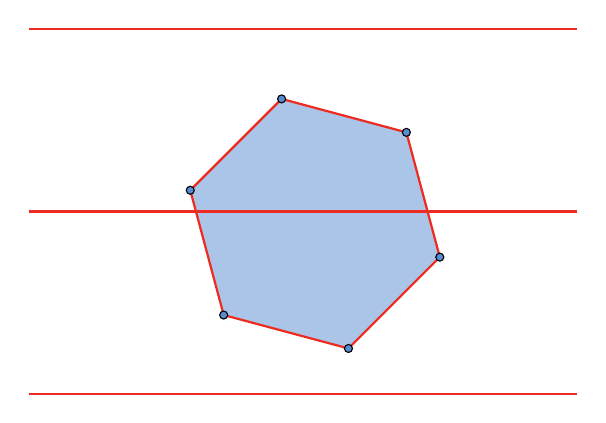
\begin{tikzpicture}[scale=0.58]
			\definecolor{qqqqff}{rgb}{0.,0.,1.}
			\definecolor{ududff}{rgb}{0.30196078431372547,0.30196078431372547,1.}
				\fill[line width=0.8pt,color=cackithi,fill=cackithi,fill opacity=0.5] (1.,3.) -- (3.,5.) -- (2.267949192431123,7.732050807568878) -- (-0.46410161513775494,8.464101615137755) -- (-2.4641016151377553,6.464101615137756) -- (-1.7320508075688794,3.7320508075688785) -- cycle;
				\draw [line width=0.8pt,color=toanhocdoisong] (1.,3.)-- (3.,5.);
				\draw [line width=0.8pt,color=toanhocdoisong] (3.,5.)-- (2.267949192431123,7.732050807568878);
				\draw [line width=0.8pt,color=toanhocdoisong] (2.267949192431123,7.732050807568878)-- (-0.46410161513775494,8.464101615137755);
				\draw [line width=0.8pt,color=toanhocdoisong] (-0.46410161513775494,8.464101615137755)-- (-2.4641016151377553,6.464101615137756);
				\draw [line width=0.8pt,color=toanhocdoisong] (-2.4641016151377553,6.464101615137756)-- (-1.7320508075688794,3.7320508075688785);
				\draw [line width=0.8pt,color=toanhocdoisong] (-1.7320508075688794,3.7320508075688785)-- (1.,3.);
				\draw [toanhocdoisong,line width=0.8pt] (-6.,6.)-- (6.,6.);
				\draw [toanhocdoisong,line width=0.8pt] (-6.,2.)-- (6.,2.);
				\draw [toanhocdoisong,line width=0.8pt] (-6.,10.)-- (6.,10.);
			
				\draw [fill=cackithi] (1.,3.) circle (2.5pt);
				\draw [fill=cackithi] (3.,5.) circle (2.5pt);
				\draw [fill=cackithi] (2.267949192431123,7.732050807568878) circle (2.5pt);
				\draw [fill=cackithi] (-0.46410161513775494,8.464101615137755) circle (2.5pt);
				\draw [fill=cackithi] (-2.4641016151377553,6.464101615137756) circle (2.5pt);
				\draw [fill=cackithi] (-1.7320508075688794,3.7320508075688785) circle (2.5pt);
		\end{tikzpicture}
		\caption{\small\textit{\color{toanhocdoisong}Hình $2$. Thả một đa giác cạnh $l$ lên tờ giấy với các đường kẻ ngang cách đều nhau.}}
		\vspace*{-10pt}
	\end{figure}
	Ta hãy tiếp tục xét một đa giác đều $N$ cạnh có độ dài mỗi cạnh bằng $l$ (Hình $2$). Ta đã biết ở trên rằng xác suất để mỗi cạnh của đa giác cắt một đường kẻ là $P(l)$. Đây cũng chính là giá trị kỳ vọng của số giao điểm của một cạnh với các đường kẻ, vì số giao điểm nói chung chỉ có thể là $0$ hoặc $1$ tương ứng với không cắt và cắt. Theo tính chất cộng tính của kỳ vọng, giá trị kỳ vọng của số giao điểm của đa giác với các đường kẻ khi thả lên tờ giấy là:
	\begin{align*}
		E &= \sum\nolimits_{i = 1}^N {P(l) = N \cdot } P(l) \\
		&= N \cdot c \cdot l = c \cdot L, \tag{$1$}
	\end{align*}
	với $L=N \cdot l$ là chu vi của đa giác đều.
	\vskip 0.1cm
	\columnbreak
	\PIbox{\textbf{\color{toanhocdoisong}Giá trị kỳ vọng}
		\vskip 0.1cm
		Trong một thí nghiệm ngẫu nhiên, nếu kết quả có giá trị $x_i$ có xác suất xảy ra là $p_i$ thì giá trị kỳ vọng của kết quả thu được được tính theo công thức:
		\setlength{\abovedisplayskip}{4pt}
		\setlength{\belowdisplayskip}{4pt}
		\begin{align*}
			E=x_1 p_1+x_2 p_2+ \cdots +x_n p_n.
		\end{align*}
		Ví dụ, với thí nghiệm gieo con xúc xắc, giá trị kỳ vọng của số chấm thu được là:
		\begin{align*}
			E=\frac{1}{6}\cdot 1 + \frac{1}{6} \cdot 2 + \cdots + \frac{1}{6}\cdot6 = 3{,5}.
		\end{align*}
		Chú ý rằng giá trị kỳ vọng có thể không trùng với một trong các giá trị có thể xảy ra. Theo định luật số lớn trong xác suất, với số lần thực hiện thí nghiệm càng lớn thì giá trị trung bình của các kết quả sẽ càng đến gần với giá trị kỳ vọng.}
	\vskip 0.1cm
	Mặt khác, nếu giữ chu vi $L$ của đa giác không đổi, khi $N \to \infty$, đa giác của ta sẽ trở thành một đường tròn có chu vi $L$ và bán kính $\dfrac{L}{2\pi}$.
	\vskip 0.1cm
	Để tính hệ số $c$, ta xét một trường hợp đặc biệt, khi đường tròn có đường kính đúng bằng khoảng cách $d$ giữa các dòng kẻ. Khi đó, ta có $L=\pi d$.
	\begin{figure}[H]
		\vspace*{-5pt}
		\centering
		\captionsetup{labelformat= empty, justification=centering}
		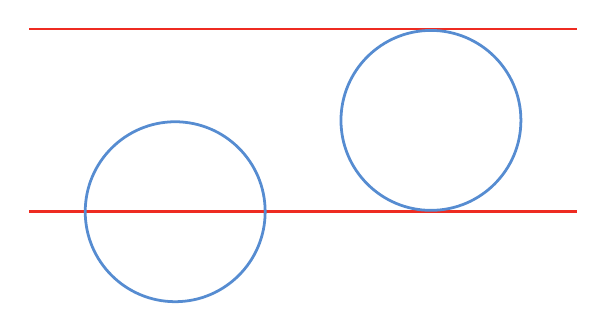
\begin{tikzpicture}[scale=0.58]
			\draw [toanhocdoisong, line width=1.pt] (-6.,6.)-- (6.,6.);
			\draw [toanhocdoisong, line width=1.pt] (-6.,10.)-- (6.,10.);
			\draw [cackithi, line width=1.pt] (2.8,8.) circle (1.97cm);
			\draw [cackithi, line width=1.pt] (-2.8,6.) circle (1.97cm);
		\end{tikzpicture}
		\caption{\small\textit{\color{toanhocdoisong}Hình $3$. Đường tròn có đường kính $d$ sẽ luôn cắt một đường kẻ tại hai điểm hoặc tiếp xúc hai đường kẻ.}}
		\vspace*{-10pt}
	\end{figure}
	Đường tròn có đường kính $d$ sẽ luôn cắt một đường kẻ tại $2$ giao điểm hoặc tiếp xúc với $2$ đường kẻ liên tiếp, do đó với đường tròn này $E=2$. Thay vào ($1$) ta có:
	\begin{align*}
		2=c\cdot\pi d
	\end{align*}
	hay $c = \dfrac{2}{\pi d}$.
	\vskip 0.1cm
	Vậy xác suất để một cây kim khi thả cắt đường nằm ngang trên giấy là 
	\begin{align*}
		P(l) = \frac{2l}{\pi d}. \tag{$2$}
	\end{align*}
	\begin{figure}[H]
		\vspace*{-5pt}
		\centering
		\captionsetup{labelformat= empty, justification=centering}
		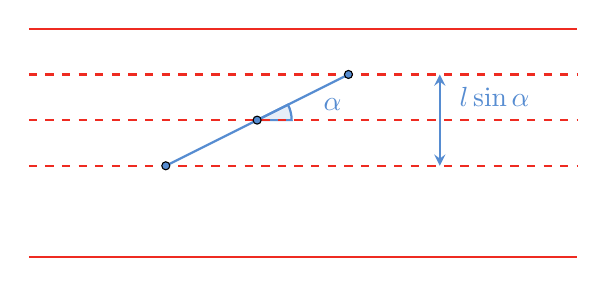
\begin{tikzpicture}[scale=0.58]
			\draw [shift={(-1.,8.)},line width=0.8pt,color=cackithi,fill=cackithi,fill opacity=0.15000000596046448] (0,0) -- (0.:0.7555063451882832) arc (0.:26.56505117707799:0.7555063451882832) -- cycle;
			\draw [toanhocdoisong,line width=0.8pt] (-6.,10.)-- (6.,10.);
			\draw [toanhocdoisong,dashed, line width=0.8pt] (-6.,9.)-- (6.,9.);
			\draw [toanhocdoisong,dashed, line width=0.8pt] (-6.,8.)-- (6.,8.);
			\draw [toanhocdoisong,dashed, line width=0.8pt] (-6.,7.)-- (6.,7.);
			\draw [toanhocdoisong, line width=0.8pt] (-6.,5.)-- (6.,5.);
			\draw [cackithi,line width=0.8pt] (-3.,7.)-- (1.,9.);
			\draw [fill=cackithi] (-3,7) circle (2.5pt);
			\draw [fill=cackithi] (1,9) circle (2.5pt);
			\draw [fill=cackithi] (-1,8) circle (2.5pt);
			\draw [cackithi,-stealth,line width=0.8pt] (3.,8.)-- (3.,9.);
			\draw [cackithi,-stealth,line width=0.8pt] (3.,8.)-- (3.,7.);
			
			\draw[color=cackithi] (0.65,8.347966297286694) node {$\color{cackithi}\alpha$};
			\draw[color=cackithi] (4.2,8.5) node {$\color{cackithi}l\sin\alpha$};
		\end{tikzpicture}
		\caption{\small\textit{\color{toanhocdoisong}Hình $4$. Chứng minh công thức $(2)$ sử dụng tích phân.}}
		\vspace*{-10pt}
	\end{figure}
	Ta cũng có thể thu được đáp án này bằng cách sử dụng tích phân. Cụ thể là ta xây dựng một mô hình xác suất cho vị trí rơi của cây kim. Gọi $\alpha$ $(0\le \alpha \le \dfrac{\pi}{2})$ là góc mà cây kim tạo với phương nằm ngang. Hình chiếu của nó theo phương vuông góc với các đường kẻ sẽ có độ dài $l\sin\alpha$, mà khoảng cách giữa hai đường kẻ là $d$, do đó xác suất để nó cắt một đường kẻ là $\dfrac{l\sin\alpha}{d}$. Coi phân bố của $\alpha$ là đều trên khoảng $[0,\dfrac{\pi}{2}]$, ta tính giá trị trung bình bằng cách lấy tích phân trên khoảng này rồi chia cho $\dfrac{\pi}{2}$ để thu được ($2$):
	\begin{align*}
		P(l) &= \frac{2}{\pi }\int_0^{\frac{\pi }{2}} {\frac{{l\sin \alpha }}{d}} d\alpha  = \frac{2}{\pi }\frac{l}{d}\left[ { - \cos \alpha } \right]|_0^{\frac{\pi }{2}}\\
		& = \frac{2}{\pi }\frac{l}{d}.
	\end{align*}
	Với cây kim có độ dài lớn hơn $d$, xác suất để nó cắt ít nhất một đường kẻ trong khoảng $\left[\arcsin\left(\dfrac{d}{l}, \dfrac{\pi}{2}\right)\right]$ sẽ luôn là $1$, do đó:
	\begin{align*}
		&P(l) \\
		= \,&\frac{2}{\pi }\left( {\int_0^{\arcsin \left( {\frac{d}{l}} \right)} {\frac{{l\sin \alpha }}{d} + } \int_{\arcsin \left( {\frac{d}{l}} \right)}^{\frac{\pi }{2}} {1d\alpha } } \right)\\
		=\,&1 \!\!+\!\! \frac{2}{\pi }\!\left( \!\!{\frac{l}{d}\!\!\left(\!\! {1 \!-\! \sqrt {\!\!1 \!-\! \frac{{{d^2}}}{{{l^2}}}} \!} \right) \!\!-\! \arcsin\! \frac{d}{l}}\! \right)\!\!.\tag{$3$}
	\end{align*}
	Bài toán này cũng được Laplace mở rộng cho trường hợp lưới trên tờ giấy là lưới chữ nhật và  tính xác suất để cây kim không cắt một đường kẻ dọc hay ngang nào. 
	\vskip 0.1cm
	Cũng chính Laplace đã đề xuất sử dụng thí nghiệm này để tính giá trị của số $\pi$. Đây cũng là khía cạnh được biết đến nhiều nhất về bài toán cây kim của Buffon. Thật vậy, nếu trong $M$ lần thả cây kim, ta thu được $m$ lần mà nó cắt một đường kẻ, công thức ($2$) cho ta:
	\begin{align*}
		\pi = \frac{2l}{d\cdot\left(\frac{m}{M}\right)},
	\end{align*}
	với $\dfrac{m}{M}$ là xác suất thực nghiệm của sự kiện cây kim cắt một đường kẻ.
	\vskip 0.1cm
	Đề xuất này của Laplace rất gần với phương pháp Monte Carlo của hơn một thế kỉ sau. Tuy vậy, về mặt thực tế, nó gập phải một số vấn đề. Nhiều thí nghiệm được tiến hành và cho kết quả của $\pi$ không quá chính xác: $3{,}1596$; $3{,}1553$; $3{,}137$.
	\vskip 0.1cm 
	Năm $1901$, Lazzarini công bố giá trị $3{,}1415929$ cho $3408$ lần thả cây kim, một giá trị khá chính xác (so với giá trị đã biết hiện nay, thì chỉ có chữ số cuối là không đúng). Tuy vậy, một số nghiên cứu đã chỉ ra kết quả này hầu như là ngụy tạo. Theo các lí thuyết về ước lượng tham số, để có độ chính xác đến $6$ chữ số sau dấu phẩy, cần phải tiến hành thí nghiệm trên $1{,}34×10^{14}$ lần chứ không phải vài nghìn lần. Đồng thời, số liệu của Lazzarini sử dụng phân số $\dfrac{355}{113}$, một số hữu tỉ được biết là một xấp xỉ tốt cho $\pi$. 
	\vskip 0.1cm
	Ngay cả với máy tính điện tử thì việc ước lượng $\pi$ bằng cách sử dụng thí nghiệm Buffon cũng không đạt được độ chính xác quá cao do việc làm tròn số trên máy tính. Đồng thời, các chữ số của $\pi$ cũng có thể được tính toán một cách chính xác hơn bởi các phương pháp khác.
	\vskip 0.1cm
	Tuy vậy, bài toán cây kim của Buffon có một ý nghĩa quan trọng trong lịch sử toán học bởi sự liên hệ giữa xác suất và hình học. Đây là một hướng tiếp cận mới khác với hướng tiếp cận xác suất sử dụng tổ hợp như truyền thống.
	\vskip 0.1cm
	\textbf{\color{toanhocdoisong}Bài tập}
	\vskip 0.1cm
	$1$. Chứng minh rằng khi cây kim vô cùng dài thì một cách hầu chắc chắn nó sẽ luôn cắt ít nhất một đường kẻ, tức là biểu thức trong ($3$) có giới hạn là $1$ khi $l\to \infty$.
	\vskip 0.1cm
	$2$. Trên tờ giấy với các đường kẻ ngang cách nhau khoảng $d$, thả ngẫu nhiên một đường tròn với bán kính $r < \dfrac{d}{2}$. Hãy tính xác suất để đường tròn cắt và không cắt các đường kẻ.
	\vskip 0.1cm
	$3$. Tương tự bài trên nhưng thả một hình vuông có cạnh $a<d$. Hãy tính xác suất để số giao điểm của các cạnh hình vuông với các đường kẻ ngang là:
	\vskip 0.1cm
	$a)$ $0$\quad\quad		$b)$ $1$\quad\quad		$c)$ $2$\quad\quad
	$d)$ $3$\quad\quad		$e)$ $4$
	\vskip 0.1cm
	Gợi ý: Xét trường hợp $a<\dfrac{d}{\sqrt{2}}$ và $a> \dfrac{d}{\sqrt{2}}$.
	\vskip 0.1cm	
	$4$. Trong thí nghiệm Buffon, với cây kim có độ dài $l>d$, hãy chứng minh giá trị kỳ vọng của số giao điểm của cây kim với các đường kẻ ngang là $E = \dfrac{2l}{\pi d}$. (Gợi ý: Gọi $N$ là số nguyên lớn nhất sao cho $d<\dfrac{l}{N}$, coi cây kim là hình gồm $N$ đoạn thẳng bằng nhau).
	\vskip 0.1cm
	$5$. Mở rộng của Laplace. Trên một lưới chữ nhật, với mỗi hình chữ nhật có chiều dài $a$ và chiều rộng $b$, thả ngẫu nhiên một cây kim chiều dài $l$ (biết rằng $l$ nhỏ hơn cả $a$ và $b$). Hãy tính xác suất để cây kim không chạm bất kỳ cạnh nào của lưới.
	\vskip 0.1cm
	$6$. Lưới Uspensky. Cho một lưới tam giác đều như hình vẽ với $d$ là chiều cao của mỗi tam giác đều. Thả một cây kim chiều dài \linebreak$l<d$ lên lưới tam giác đều này. Hãy tính xác suất để số giao điểm của cây kim với các đường trong lưới là:
	\vskip 0.1cm
	\quad\quad$a)$ $0$\quad\quad		$b)$ $1$\quad\quad		$c)$ $2$	\quad\quad	$d)$ $3$
	\begin{figure}[H]
		\vspace*{5pt}
		\centering
		\captionsetup{labelformat= empty, justification=centering}
		\includegraphics[width=1\linewidth]{6}
		\vspace*{-15pt}
	\end{figure}
	$7$. Bài toán sợi mì của Buffon. Trên một tờ giấy với các đường kẻ ngang song song cách nhau khoảng $d$, ném ngẫu nhiên một sợi mì ướt có độ dài $l$. Chứng minh rằng giá trị kì vọng của số giao điểm của sợi mì với các đường kẻ ngang là $E=\dfrac{2l}{\pi d}$. Giả sử rằng khi ném sợi mì, chiều dài của nó không đổi nhưng nó có thể uốn thành một đường cong bất kỳ.
	\vskip 0.1cm
	\textbf{\color{toanhocdoisong}$\pmb{2.}$ Đo độ dài bằng phương pháp ngẫu nhiên}
	\vskip 0.1cm
	Với một số thay đổi, thí nghiệm của Buffon có thể được sử dụng để giải quyết một vấn đề thực tế trong khoa học: đo độ dài của rễ cây (Newman, $1966$). Xét một bản thủy tinh mà trên đó một mẫu vật (ví dụ rễ cây) được trải phẳng. Khi quan sát mẫu vật qua kính hiển vi, người ta sử dụng một thị kính với một đường sợi tóc để soi các vùng khác nhau của bản thủy tinh.
	\vskip 0.1cm
	Với mỗi lần quan sát, thị kính được quay một góc bất kì và đường sợi tóc cũng được quay theo. Sau đó, số giao điểm của đường sợi tóc với rễ cây sẽ được ghi lại. Cách thức này được lặp lại nhiều lần với các vị trí quan sát ngẫu nhiên khác nhau trên bản thủy tinh. Để tiện lợi hơn, ta có thể đặt bản thủy tinh trên một tấm giấy với các điểm ngẫu nhiên đã được đánh dấu trước. Các điểm quan sát cũng có thể là một lưới ô vuông các điểm cách đều.
	\begin{figure}[H]
%		\vspace*{5pt}
		\centering
		\captionsetup{labelformat= empty, justification=centering}
		\includegraphics[width=1\linewidth]{7}
		\includegraphics[width=1\linewidth]{8}
		\caption{\small\textit{\color{toanhocdoisong}Hình $5$. Trên: Thị kính của kính hiển vi có đường sợi tóc (đường thẳng đứng). Dưới: minh họa phép đo độ dài rễ cây (màu xanh) với các vị trí và góc quay khác nhau của đường sợi tóc (màu đỏ). Số lượng đường sợi tóc trong hình chỉ mang tính minh họa, trong thực tế, cấu trúc rễ cây càng phức tạp thì số lượng đường sợi tóc cần sử dụng lại càng nhiều. Mỗi lần quan sát qua kính, ta chỉ thấy được một vùng hình tròn có đường kính là đường sợi tóc.}}
		\vspace*{-10pt}
	\end{figure}
	Về mặt bản chất, thay vì đếm số giao điểm của cây kim được thả ngẫu nhiên với các đường kẻ ngang, ta đếm số giao điểm của các đường sợi tóc được phân bố ngẫu nhiên với mẫu vật rễ cây (gồm nhiều đường cong) trên bản thủy tinh.
	\vskip 0.1cm
	Độ dài của rễ cây có thể được tính theo công thức:
	\begin{align*}
		R= \frac{\pi N A}{2H},	\tag{$4$}
	\end{align*}
	với $N$ là số giao điểm đã được đếm, $A$ là diện tích bản thủy tinh và $H$ là tổng độ dài của tất cả các đường sợi tóc.
	\vskip 0.1cm
	Thật vậy, xét một đoạn rễ cây $PQ$ có chiều dài $\Delta R$ và một đường sợi tóc $MN$ chiều dài $h$. Nếu khoảng cách từ trung điểm $D$ của $PQ$ đến $MN$ lớn hơn $\dfrac{1}{2}\Delta R$ thì $PQ$ và $MN$ chắc chắn không cắt nhau. Miền giới hạn này được biểu diễn bằng đường nét đứt trong hình. Giả sử $\dfrac{\Delta R}{h}$ là nhỏ, diện tích miền này có thể được xấp xỉ bằng $\Delta R \cdot h$. Do $MN$ được phân bố ngẫu nhiên trên bản thủy tinh, xác suất để $D$ nằm trong miền này là $\dfrac{\Delta R \cdot h}{A}$.
	\vskip 0.1cm
	Khi $D$ nằm trong miền cách $MN$ một khoảng không quá $\dfrac{1}{2}\Delta R$, khoảng cách từ $D$ đến $MN$ cần phải không lớn hơn $\dfrac{1}{2}\Delta R |\sin \theta |$, với $\theta$ là góc tạo bởi hai đường thẳng $PQ$ và $MN$, để $PQ$ và $MN$ cắt nhau. Xác suất để $PQ$ và $MN$ cắt nhau khi $D$ đã nằm trong miền trên là:
	\begin{align*}
		\frac{\frac{1}{2}\Delta R|\sin\theta|}{\frac{1}{2}\Delta R} = |\sin\theta|.
	\end{align*}
	Do đó, theo công thức nhân xác suất, xác suất để $PQ$ và $MN$ cắt nhau là:
	\begin{align*}
		p = \frac{\Delta R\cdot h}{A} |\sin\theta|.
	\end{align*}
	\begin{figure}[H]
		\vspace*{-5pt}
		\centering
		\captionsetup{labelformat= empty, justification=centering}
		\includegraphics[width=1\linewidth]{9}
		\caption{\small\textit{\color{toanhocdoisong}Hình $6$. Đoạn rễ cây $PQ$ và đường sợi tóc $MN$.}}
		\vspace*{-10pt}
	\end{figure}
	Tổng độ dài của các đoạn sợi tóc được phân bố ngẫu nhiên trên miền diện tích $A$ là $H$. Các góc $\theta$ cũng nhận giá trị ngẫu nhiên trong khoảng $[0,2\pi]$ nên giá trị kì vọng của số giao điểm của $PQ$ với các đường sợi tóc là:
	\begin{align*}
		\frac{1}{2\pi}\int_0^{2\pi}{\frac{{\Delta R \cdot H}}{A}}|\sin\theta|d\theta= \frac{2\left(\Delta R \cdot H\right)}{\pi A}.
	\end{align*}
	Coi rễ cây là một hình với nhiều đoạn có độ dài $\Delta R$, ta được giá trị kì vọng của số giao điểm của rễ cây với tất cả các đường sợi tóc là:
	\begin{align*}
		N = \frac{2RH}{\pi A}.
	\end{align*}
	Do $N$ là giá trị kỳ vọng nên khi đo đạc người ta cần phải tiến hành nhiều lần quan sát với các vị trí ngẫu nhiên của đường sợi tóc để kết quả thí nghiệm gần với giá trị của $N$ trong công thức.
	\vskip 0.1cm
	Ví dụ, với bản thủy tinh $10\times 20$ cm; tiến hành quan sát $40$ lần, độ dài đường sợi tóc (đường kính của thị trường vùng quan sát được) là $1{,}88$ cm; số giao điểm quan sát được là $344$ thì tổng độ dài của rễ cây là:
	\begin{align*}
		R - \frac{\pi \cdot 344\cdot 10 \cdot 20}{2\cdot40 \cdot1{,}88} = 1436 \text{ cm}.
	\end{align*}
	Cách đo độ dài này đã được các nhà thực vật học sử dụng trong nhiều thập kỉ mãi cho đến gần đây mới được thay thế bởi các phần mềm xử lí ảnh từ các camera có độ phân giải cao.
	\vskip 0.1cm
	\textbf{\color{toanhocdoisong}$\pmb{3.}$ Kiến biết đo diện tích bằng xác suất?}
	\vskip 0.1cm
	Phương pháp đo độ dài ở phần trước cũng có thể được biến đổi để tiến hành đo diện tích.
	\vskip 0.1cm
	Một nghiên cứu khá thú vị trên loài kiến \textit{Leptothorax albipennis} đưa ra giả thuyết rằng loài kiến này đã sử dụng xác suất để tính diện tích khi chọn tổ (kiến thường cố gắng chọn tổ có diện tích lớn nhất trong các vị trí khảo sát) (Mallon \& Franks, $2000$).
	\vskip 0.1cm
	Khi sử dụng camera để theo dõi kiến trinh sát trong phòng thí nghiệm, người ta thấy trong lần thứ nhất đến một vị trí để khảo sát, con kiến sẽ đi một cách ngẫu nhiên trong hộp theo một đường cong bao phủ phần lớn các vị trí trong hộp (gọi là đường cong $L$). Trong những lần tiếp theo (thường nó sẽ quay lại lần thứ hai hoặc có thể là lần thứ $3$), nó sẽ đi một đường cong đơn giản hơn (gọi là đường cong $S$). Đồng thời, khi đến các vị trí đã đi qua (kiến khi di chuyển có thể tiết ra pheromone để đánh dấu đường đi của mình), tức là các giao điểm của $L$ và $S$, kiến dành thời gian lâu hơn nhiều.
	\begin{figure}[H]
		\vspace*{-5pt}
		\centering
		\captionsetup{labelformat= empty, justification=centering}
		\includegraphics[width=0.65\linewidth]{10}
		\caption{\small\textit{\color{toanhocdoisong}Hình $7$. Từ trên xuống: Đường đi của kiến trinh sát khi khảo sát tổ được camera ghi lại trong lần khảo sát thứ nhất, thứ hai và thứ ba.}}
		\vspace*{-10pt}
	\end{figure}
	Theo các tác giả, số giao điểm của $L$ và $S$ được kiến trinh sát sử dụng để đánh giá diện tích của một vị trí làm tổ. Trong công thức ($4$), nếu ta thay các đường sợi tóc bằng một đường cong $L$ và rễ cây $R$ bằng đường cong $S$, công thức này vẫn đúng và diện tích có thể được xấp xỉ theo 
	\begin{align*}
		A = \frac{2SL}{\pi N}, \tag{$5$}
	\end{align*}
	với $N$ là số giao điểm của $S$ và $L$.
	\vskip 0.1cm
	Để kiểm chứng việc này, thí nghiệm được tiến hành với nhiều con kiến trinh sát khác nhau trên các loại hộp để làm tổ như trong hình vẽ.
	\vskip 0.1cm
	Trong thí nghiệm để chọn giữa hai tổ cùng chu vi (hình $8a$ và hình $8c$), kiến luôn chọn tổ có diện tích lớn hơn sau khi khảo sát cả hai. Do đó, diện tích chứ không phải chu vi mới là tiêu chí chọn tổ. Vì các tổ có một tấm chắn ở giữa (hình $8d$) cũng được chọn với khả năng tương tự như tổ bình thường, cho thấy số lần va chạm với chướng ngại vật trong tổ cũng không phải nhân tố quyết định.
	\begin{figure}[H]
		\vspace*{-5pt}
		\centering
		\captionsetup{labelformat= empty, justification=centering}
		\includegraphics[width=1\linewidth]{11}
		\caption{\small\textit{\color{toanhocdoisong}Hình $8$. Các loại tổ được sử dụng trong thí nghiệm về việc chọn tổ của kiến trinh sát. $a)$ tổ tiêu chuẩn; $b)$ tổ đồng dạng và có diện tích bằng một nửa tổ tiêu chuẩn; $c)$ tổ có diện tích bằng một nửa tổ tiêu chuẩn nhưng có cùng chu vi; $d)$ tổ tiêu chuẩn có tấm chắn ở giữa; $e)$ tổ dạng $b$ với một nửa được phủ các tấm đệm có thể nhấc ra.}}
		\vspace*{-10pt}
	\end{figure}
	Thí nghiệm cũng cho thấy khi kiến trở lại lần thứ hai, nếu tổ đã được thay bằng một tổ mới hoặc một tổ đã được một con kiến khác đi qua, nó sẽ tiến hành khảo sát lại như là đang đi qua lần thứ nhất. Điều này cho thấy trong lần khảo sát thứ nhất, kiến sẽ lưu lại pheromone đánh dấu đường đi và pheromone này đặc trưng cho từng cá thể. Việc này cũng cho phép các con kiến không làm ảnh hưởng đến quá trình khảo sát của nhau khi một vị trí có thể được nhiều hơn một con kiến đến thăm dò.
	\vskip 0.1cm
	Nếu kiến trở lại lần thứ ba hoặc sau đó, thời gian nó tiến hành khảo sát cũng không khác nhiều lắm so với lần thứ hai, do đó có thể thấy pheromone chỉ được rải ở lần thăm dò thứ nhất còn các lần lặp lại sau để tăng độ chính xác của việc ước lượng.
	\vskip 0.1cm
	Loại tổ trong hình $8e$ được thiết kế đồng dạng với tổ trong hình $8a$ nhưng có diện tích bằng một nửa. Đồng thời, ở nền của loại tổ này, một nửa diện tích là các tấm đệm có thể lấy ra. Sau khi kiến khảo sát tổ dạng này lần thứ nhất, người ta sẽ lấy các tấm đệm ra trước khi kiến quay lại lần thứ hai. Khi kiến trở lại, do các vị trí có đệm bị lấy ra không còn pheromone nên số giao điểm của đường đi của nó trong lần thứ hai với đường đi trong lần thứ nhất sẽ giảm một nửa. Trong thí nghiệm chọn giữa tổ dạng $8a$ và dạng $8e$, một nửa số kiến chọn $8e$ dù diện tích chỉ có một nửa. Thí nghiệm với kích thước tổ lớn gấp đôi cho thấy khoảng cách $L$ của mỗi con kiến là không đổi giữa các tổ với diện tích khác nhau. Kết hợp với với ($5$), có thể thấy thấy kiến đánh giá diện tích theo tỉ lệ nghịch với tần số gặp giao điểm $\dfrac{N}{S}$.
	\vskip 0.1cm
	Việc nghiên cứu những thuật toán liên quan đến hành vi của kiến không chỉ có ý nghĩa về mặt sinh học mà còn có nhiều ứng dụng khác, ví dụ như trong việc lập trình điều khiển hành vi của robot.
	\vskip 0.1cm
	$\pmb{4.}$ \textbf{\color{toanhocdoisong}Lời kết}
	\vskip 0.1cm
	Lĩnh vực xác suất hình học còn có nhiều bài toán khác có giá trị về cả mặt lý thuyết lẫn thực tiễn. Pi cũng sẽ tiếp tục giới thiệu các bài toán này đến với độc giả trong tương lai không xa.
	\vskip 0.1cm
	\textbf{\color{toanhocdoisong}Tài liệu tham khảo}
	\vskip 0.1cm
	[$1$] Aigner, M., \& Ziegler, G. ($2004$). \textit{Proof from} THE BOOK. Springer--Verlag.
	\vskip 0.1cm
	[$2$] Mallon, E. B., \& Franks, N. R. ($2000$). Ants estimate area using Buffon's needle. \textit{Proc. R. Soc. Lond.} B($267$), $765-770$.
	\vskip 0.1cm
	[$3$] Mugford, S. T., Mallon, E. B., \& Franks, N. R. ($2001$). The accuracy of Buffon's needle: a rule of thumb used by ants to estimate area. \textit{Behavioral Ecology}, $12(6)$, $655-658$.
	\vskip 0.1cm
	[$4$] Newman, E. I. ($1966$). A Method of Estimating the Total Length of Root in a Sample. \textit{Journal of Applied Ecology}, $139-145$.
	\vskip 0.1cm
	[$5$] Ramaley, J. F. ($1969$). Buffon's Noodle Problem. \textit{The American Mathematical Monthly}, $78(8)$, $916-918$.
\end{multicols}
%	\newpage



%	\setcounter{figure}{0}
%	\thispagestyle{duongvaotoanhocnone}
\pagestyle{duongvaotoanhoc}
\everymath{\color{duongvaotoanhoc}}
\graphicspath{{../duongvaotoanhoc/pic/}}
\blfootnote{$^1$\color{duongvaotoanhoc}Images des Mathématiques, http://images.math.cnrs.fr/Les-tresses-de-la-topologie-a-la-cryptographie.html.}
\blfootnote{$^2$\color{duongvaotoanhoc}Giáo sư, Đại học Bourgogne, Pháp.}
\blfootnote{$^3$\color{duongvaotoanhoc}Viện Toán học.}
\begingroup
\AddToShipoutPicture*{\put(0,616){\includegraphics[width=19.3cm]{../bannerduongvao}}}
\AddToShipoutPicture*{\put(78,532){\includegraphics[scale=1]{../tieude.pdf}}}
\centering
\endgroup

\vspace*{175pt}

\tikzstyle{start} = [rectangle, rounded corners, minimum height=1cm,text centered, draw=black, fill=red!30]

\tikzstyle{end} = [rectangle, rounded corners, minimum height=1cm,text centered, draw=black, fill=blue!30]

\tikzstyle{mid} = [rectangle, rounded corners, minimum height=1cm,text centered, draw=black, fill=green!30]

\begin{multicols}{2}	
	$\pmb{1.}$ \textbf{\color{duongvaotoanhoc}Mở đầu}
	\vskip 0.1cm
	\textbf{\color{duongvaotoanhoc}Từ dải bện...}
	\vskip 0.1cm
	Dải bện đã tồn tại từ nhiều thế kỷ và được sử dụng khắp nơi vì mục đích trang trí cũng như trong đời sống, chẳng hạn trong sản xuất dây thừng hoặc dây cáp. Một dải bện có thể gồm ba sợi, hay cọng, được tết với nhau: cọng trái được vắt qua cọng giữa, rồi đến cọng phải, rồi lại cọng trái, rồi lại cọng phải, cứ thế lặp đi lặp lại (xem Hình $1$). Nhưng ``dải bện" cũng được dùng để chỉ mọi sự đan hay tết của nhiều cọng dây theo một cách nhất định. Trong Hình $2$ và Hình $3$ là một số thí dụ về các dải bện trang trí.
	\begin{figure}[H]
		\vspace*{-5pt}
		\centering
		\captionsetup{labelformat= empty, justification=centering}
		\includegraphics[width= 1\linewidth]{fig_01}
		\caption{\small\textit{\color{duongvaotoanhoc}Hình $1$. Dải bện cổ điển với ba cọng dây.}}
		\vspace*{-10pt}
	\end{figure}
	\begin{figure}[H]
		\vspace*{-10pt}
		\centering
		\captionsetup{labelformat= empty, justification=centering}
		\includegraphics[width= 1\linewidth]{fig_02}
		\caption{\small\textit{\color{duongvaotoanhoc}Hình $2$. Một dải bện trang trí.}}
		\vspace*{-5pt}
	\end{figure}
	\textbf{\color{duongvaotoanhoc}... đến lý thuyết bện}
	\vskip 0.1cm
	Các nhà toán học mô tả các dải bện bằng các mô hình trừu tượng, những đối tượng trung tâm của một lý thuyết toán học có tên ``lý thuyết bện". Lý thuyết này đóng một vai trò trung tâm trong toán học và len lỏi vào trong nhiều ngành toán học, cũng như các khoa học khác như vật lý, sinh học, tin học và mật mã.
	\begin{figure}[H]
		\vspace*{-10pt}
		\centering
		\captionsetup{labelformat= empty, justification=centering}
		\includegraphics[width= 0.75\linewidth]{fig_03a}
		\caption{\small\textit{\color{duongvaotoanhoc}Hình $3$. Một dải bện trang trí khác.}}
		\vspace*{-10pt}
	\end{figure}
	Bài viết này nhằm đem đến cho độc giả không làm toán một cái nhìn bao quát về lý thuyết bện. Chúng tôi sẽ đưa ra định nghĩa bện trong toán học, sau đó minh họa ứng dụng của chúng trong ba lĩnh vực: lý thuyết nút (toán học), lý thuyết thuật toán (toán học và tin học), và lý thuyết mật mã (toán học, tin học và viễn thông). Ngoài ra, chúng còn nhiều ứng dụng và tương tác qua lại khác với các phần khác của toán học, và với cả, chẳng hạn, vật lý thiên văn. Thực vậy, các đường từ trường trong khí quyển Mặt Trời tạo thành các dải bện mà độ phức tạp có liên hệ trực tiếp đến cường độ của từ trường.
	\vskip 0.1cm
%	Lý thuyết bện là một lĩnh vực nghiên cứu rất tích cực ở Pháp, được tổ chức xung quanh nhóm nghiên cứu GDR TRESSES được thành lập năm $2020$ bởi Patrick Dehornoy.
%	\begin{tBox}
%		\begin{wrapfigure}{l}{0.4\linewidth}
%			\vspace*{-15pt}
%			\centering
%			\captionsetup{labelformat= empty, justification=centering}
%			\hspace*{2pt}\includegraphics[width= 1.05\linewidth]{fig_Dehornoy}
%			\caption{\small\textit{\color{duongvaotoanhoc}Patrick Dehornoy.}}
%			\vspace*{-10pt}
%		\end{wrapfigure}
%		Patrick Dehornoy ($1952-2019$) là nhà toán học Pháp được biết đến vì những công trình trong lý thuyết tập hợp và lý thuyết bện. Ông nguyên là giáo sư tại Đại học Caen và là thành viên kỳ cựu của Viện Đại học Pháp (Institut Universitaire de France).
%	\end{tBox}
	\vskip 0.1cm
	$\pmb{2.}$ \textbf{\color{duongvaotoanhoc}Dải bện trong toán học}
	\vskip 0.1cm
	\textbf{\color{duongvaotoanhoc}Thế nào là một dải bện trong toán học?}
	\vskip 0.1cm
	\textit{Lý thuyết bện} tách khái niệm bện khỏi những dải bện mà ta vẫn thường nghĩ đến. Trước tiên, ta cố định một số tự nhiên $n$. Để tiện trình bày, ta sẽ lấy $n = 4$, mặc dù tất cả những gì được mô tả tiếp theo đây đúng với mọi giá trị của $n$. Chúng ta lấy hai tập hợp, mỗi tập hợp có $4$ vật (chẳng hạn những cái đinh) và để chúng trên bàn thành hai hàng dọc đối diện nhau (các chấm đen trong hình). Sử dụng bốn sợi dây, mà ta gọi là cọng, ta nối mỗi vật trong tập hợp thứ nhất với một vật trong tập hợp thứ hai. Một kết nối như vậy được gọi là một dải bện. Các cọng có thể vắt qua nhau, nhưng không được vòng ngược lại. Kết nối trong Hình $5$ không phải là một dải bện (theo nghĩa toán học).
	\begin{figure}[H]
		\vspace*{-7pt}
		\centering
		\captionsetup{labelformat= empty, justification=centering}
		\includegraphics[width= 0.465\linewidth]{fig_04}\quad
		\includegraphics[width= 0.465\linewidth]{fig_05}
		\caption{\small\textit{\color{duongvaotoanhoc}Hình $4$. Một dải bện \hspace*{18pt} Hình $5$. Đây không \hspace*{10pt}\\
				\hspace*{20pt}toán học.\hspace*{45pt} phải một dải bện. }}
		\vspace*{-10pt}
	\end{figure}	
	Trong Hình $6$ là hai dải bện khác nhau. Trong khi đó, hai dải bện trong Hình $7$ là giống nhau, vì chúng có thể nhận được từ nhau bằng cách ``xê dịch" các cọng.
	\begin{figure}[H]
		\vspace*{-5pt}
		\centering
		\captionsetup{labelformat= empty, justification=centering}
		\includegraphics[width= 1\linewidth]{fig_06}
		\caption{\small\textit{\color{duongvaotoanhoc}Hình $6$. Hai dải bện khác nhau.}}
		\vspace*{-5pt}
	\end{figure}
	\begin{figure}[H]
		\vspace*{5pt}
		\centering
		\captionsetup{labelformat= empty, justification=centering}
		\includegraphics[width= 1\linewidth]{fig_07}
		\caption{\small\textit{\color{duongvaotoanhoc}Hình $7$. Hai dải bện giống nhau.}}
		\vspace*{-10pt}
	\end{figure}
	Một dải bện cũng có thể được coi như một chuỗi các đường đi của $4$ hạt không gặp nhau. Ở đây, tập hợp các điểm xuất phát trùng với tập hợp các điểm đến. Thí dụ, các quỹ đạo của $4$ hạt được thể hiện ở nửa trên của Hình $8$ tương ứng với dải bện ở nửa dưới. Một cách nôm na, các dải bện có thể được xem như những điệu nhảy mà ở đó, mỗi vũ công kết thúc ở vị trí của một vũ công khác.
	\begin{figure}[H]
		\vspace*{-8pt}
		\centering
		\captionsetup{labelformat= empty, justification=centering}
		\includegraphics[width= 0.45\linewidth]{fig_08}
		\caption{\small\textit{\color{duongvaotoanhoc}Hình $8$. Hai cách nhìn của cùng một dải bện.}}
		\vspace*{-10pt}
	\end{figure}
	\textbf{\color{duongvaotoanhoc}Ghép các dải bện}
	\vskip 0.05cm
	Từ hai dải bện $\alpha$ và $\beta$, ta có thể xây dựng một phép thứ ba, ký hiệu là $\alpha \beta$ và được gọi là dải bện hợp thành của $\alpha$ và $\beta$, bằng cách ghép chúng với nhau. Trong Hình $9$ là hai dải bện (bên trên) và hợp thành của chúng (bên dưới).
	\begin{figure}[H]
		\vspace*{-8pt}
		\centering
		\captionsetup{labelformat= empty, justification=centering}
		\includegraphics[width= 1\linewidth]{fig_09}
		\caption{\small\textit{\color{duongvaotoanhoc}Hình $9$. Hợp thành của hai dải bện.}}
		\vspace*{-5pt}
	\end{figure}
	Một thí dụ khác về phép hợp thành được minh họa trong Hình $10$.
	\begin{figure}[H]
		\vspace*{-8pt}
		\centering
		\captionsetup{labelformat= empty, justification=centering}
		\includegraphics[width= 0.97\linewidth]{fig_10}
		\caption{\small\textit{\color{duongvaotoanhoc}Hình $10$. Hợp thành của hai dải bện khác.}}
		\vspace*{-10pt}
	\end{figure}
	Bạn đọc có kinh nghiệm hẳn đã để ý rằng dải bện $\alpha \beta$ có thể khác với dải bện $\beta \alpha$: điều này xảy ra với thí dụ trong Hình $9$, nhưng không đúng với thí dụ trong Hình $10$.
	
	Dải bện trong Hình $11$ được gọi là \textit{dải bện tầm thường}. Dễ thấy hợp của một dải bện $\alpha$ bất kỳ với dải bện tầm thường, từ bên trái hay từ bên phải, vẫn là $\alpha$.
	\begin{figure}[H]
		\vspace*{-5pt}
		\centering
		\captionsetup{labelformat= empty, justification=centering}
		\includegraphics[width= 0.46\linewidth]{fig_11}
		\caption{\small\textit{\color{duongvaotoanhoc}Hình $11$. Dải bện tầm thường.}}
		\vspace*{-10pt}
	\end{figure}
	Nếu ta đặt một tấm gương vuông góc với mặt bàn ở cạnh hàng đinh thứ hai, ảnh phản chiếu trong gương của dải bện $\alpha$ được gọi là dải bện đối xứng của $\alpha$ (xem Hình $12$). Hợp thành của một dải bện với dải bện đối xứng của nó là dải bện tầm thường. Bạn đọc có thể dễ dàng kiểm chứng với thí dụ trong Hình~$12$.
	\begin{figure}[H]
		\vspace*{-8pt}
		\centering
		\captionsetup{labelformat= empty, justification=centering}
		\includegraphics[width= 0.97\linewidth]{fig_12}
		\caption{\small\textit{\color{duongvaotoanhoc}Hình $12$. Một dải bện và dải bện đối xứng của~nó.}}
		\vspace*{-5pt}
	\end{figure}
	\textbf{\color{duongvaotoanhoc}Từ dải bện đến nhóm bện}
	\vskip 0.1cm
	Những dải bện, như chúng ta vừa định nghĩa, cùng với phép hợp thành tạo thành cái mà các nhà toán học gọi là \textit{nhóm bện}. Chúng ta có một nhóm bện [gồm các dải bện có] hai cọng, một nhóm bện ba cọng, v.v. Nhóm bện một cọng chỉ gồm dải bện tầm thường, vì một cọng thì không thể được bện, dù nó có thể được buộc thắt nút (xem Hình $13$).
	\begin{figure}[H]
		\vspace*{-5pt}
		\centering
		\captionsetup{labelformat= empty, justification=centering}
		\includegraphics[width= 0.5\linewidth]{fig_13}
		\caption{\small\textit{\color{duongvaotoanhoc}Hình $13$. Cọng buộc thắt nút.}}
		\vspace*{-10pt}
	\end{figure}
	Phép hợp thành của các dải bện tuân theo một số quy tắc mà đối với các nhà toán học cũng quan trọng không kém, nếu không nói là hơn, chính các dải bện.
	Nguồn gốc của lý thuyết bện.
	\begin{tBox}
		\begin{wrapfigure}{l}{0.4\linewidth}
			\vspace*{-15pt}
			\centering
			\captionsetup{labelformat= empty, justification=centering}
			\includegraphics[width= 1.1\linewidth]{fig_Artin}
			\caption{\small\textit{\color{duongvaotoanhoc}Emil Artin}}
			\vspace*{-15pt}
		\end{wrapfigure}
		Emil Artin ($1898-1962$) là nhà toán học người Áo. Ông làm việc ở Đức (chủ yếu ở Hamburg) đến năm $1937$. Ông sang Mỹ và làm giáo sư tại Đại học Indiana từ năm $1938$ đến năm $1946$, rồi tại Đại học Princeton từ năm $1946$ đến năm $1958$. Ông là một trong những nhà đại số xuất sắc nhất thế kỷ $20$. Đặc biệt, ông là người khai sinh lý thuyết bện.
	\end{tBox}
	Nghiên cứu toán học về các dải bện thường được cho là bắt đầu từ một bài báo năm $1925$ của Emil Artin, trong đó ông mô tả khái niệm dải bện dưới nhiều khía cạnh khác nhau, cái thì hiển nhiên như ``một chuỗi các cọng dây được kéo căng và quấn vào nhau", những cái khác toán học hơn, chẳng hạn như nhóm được cho bởi ``các phần tử sinh và các quan hệ", hay như ``nhóm các tự đẳng cấu của một nhóm tự do", hay như  ``nhóm các phép đẳng luân của một đĩa bị thủng". Chính sự đa dạng của các cách tiếp cận khác nhau này tạo nên tính hấp dẫn của các nhóm bện.
	\vskip 0.1cm
	$\pmb{3.}$ \textbf{\color{duongvaotoanhoc}Từ dải bện đến lý thuyết nút}
	\vskip 0.1cm
	\textbf{\color{duongvaotoanhoc}Nút trong toán học là gì?}
	\vskip 0.1cm
	Một \textit{nút} trong toán học là một vòng dây khép kín (không có hai đầu, xem Hình $14$). Một \textit{cuộn dây gồm hai thành phần} được tạo bởi hai vòng dây khép kín (xem Hình $15$), một \textit{cuộn dây gồm ba thành phần} được tạo bởi ba vòng dây khép kín, v.v. \textit{Lý thuyết nút} là nhánh của tô--pô nghiên cứu các nút và các cuộn. Trong tô--pô, hình cầu không phân biệt với hình lập phương, còn cái bánh vòng và tách trà là một. Người ta không xét đến các thuộc tính như độ dài hay góc, mục đích là hiểu các tính chất bất biến đối với sự xoắn, kéo dãn hay nén.
	\begin{figure}[H]
		\vspace*{-10pt}
		\centering
		\captionsetup{labelformat= empty, justification=centering}
		\hspace*{5pt}\includegraphics[height= 0.45\linewidth]{fig_14}\hspace*{25pt}
		\includegraphics[height= 0.45\linewidth]{fig_15}
		\caption{\small\textit{\color{duongvaotoanhoc}\hspace*{10pt}Hình $14$. Một nút. \hspace*{10pt} Hình $15$. Một cuộn dây\\ \hspace*{96pt}gồm hai thành phần.}}
		\vspace*{-10pt}
	\end{figure}
	Ngoài toán học, đặc biệt là tô--pô, lý thuyết nút có những ứng dụng trong các bài toán sinh học và hóa học. Chẳng hạn, nó được dùng trong nghiên cứu các phân tử đồng phân (có cùng công thức hóa học nhưng được sắp xếp khác nhau) hoặc trong nghiên cứu về tác động của một số enzyme đối với ADN.
	\vskip 0.1cm
	\textbf{\color{duongvaotoanhoc}Nguồn gốc của lý thuyết nút}
	\vskip 0.1cm
	Đóng góp đáng kể đầu tiên vào lý thuyết nút có lẽ là của Sir William Thomson (tức Kelvin) với thuyết ``xoáy nguyên tử" của ông. Năm $1867$, sau khi quan sát các vòng khói được tạo ra từ thí nghiệm của Peter Tait, nhà vật lý người Scotland, Thomson kết luận rằng các nguyên tử là những nút của ``những cuộn xoáy trong ê--te truyền ánh sáng". Theo đó, các nguyên tố hóa học ứng với các nút hoặc cuộn dây. Từ ý tưởng này, Peter Tait bắt đầu phân loại các nút, với niềm tin rằng ông đang tạo ra một bảng nguyên tố hóa học.
	\begin{tBox}
		\begin{wrapfigure}{l}{0.4\linewidth}
			\vspace*{-15pt}
			\centering
			\captionsetup{labelformat= empty, justification=centering}
			\hspace*{2pt}\includegraphics[width= 1.1\linewidth]{fig_William}
			\caption{\small\textit{\hspace*{2pt}\color{duongvaotoanhoc}William~Thomson.}}
			\vspace*{-10pt}
		\end{wrapfigure}
		Sir William Thomson ($1824-1907$) là nhà vật lý học, nhà toán học và kỹ sư người Scotland. Ông được coi là một trong những nhà vật lý học hàng đầu của thế kỷ~$19$.
	\end{tBox}
	\textbf{\color{duongvaotoanhoc}Bài toán phân biệt hai nút}
	\vskip 0.05cm
	Bài toán trung tâm của lý thuyết nút là phân biệt, và xa hơn là phân loại, các nút. Phân biệt có nghĩa là quyết định xem liệu hai hình vẽ nút (hoặc cuộn dây) có biểu diễn cùng một nút (hoặc cuộn dây) hay không. Trong những năm $1920$, hai nhà toán học Mỹ Alexander và Briggs và nhà toán học Đức Reidemeister, độc lập với nhau, đề xuất một thuật toán giải quyết một phần bài toán này. Thuật toán này có thể trả lời khẳng định nếu hai hình vẽ biểu diễn cùng một nút (hoặc cuộn), nhưng nó không trả lời trong trường hợp ngược lại. Nói cách khác, ta có thể nói hai nút giống nhau hay không, nhưng không thể nói hai nút có khác nhau hay không. Độc giả có thể cảm thấy điều này thật vô lý, nhưng nó là một nghịch lý thường thấy trong toán học. Hãy tưởng tượng bạn đang chờ ai đó. Bạn tự nhủ: ``Nếu cậu ấy đến, đó đúng là một người bạn." Nhưng nếu người đó không đến, bạn sẽ không biết đó có phải một người bạn hay không.
	\vskip 0.05cm
	Để phân biệt các nút, người ta sử dụng những cái mà các nhà toán học gọi là những \textit{bất biến}. Người ta gán cho mỗi hình vẽ cái nút một đối tượng (thường là một số hoặc một đa thức) chỉ phụ thuộc vào cái nút mà không phụ thuộc vào cách nó được vẽ. Nếu hai nút có những bất biến khác nhau thì chúng là hai nút khác nhau. Nếu không, ta chưa thể kết luận được gì.
	\begin{tBox}
				\begin{wrapfigure}{l}{0.4\linewidth}
							\vspace*{-15pt}
							\centering
							\captionsetup{labelformat= empty, justification=centering}
							\hspace*{2pt}\includegraphics[width= 1.1\linewidth]{fig_Alexander}
							\caption{\small\textit{\color{duongvaotoanhoc}Alexander.}}
							\vspace*{-10pt}
						\end{wrapfigure}
				James W. Alexander ($1888-1971$) là một nhà toán học nổi tiếng người Mỹ.  Ông là một trong những người tiên phong của tô--pô đại số và lý thuyết nút. 
				Ông cũng là một nhà leo núi cừ khôi,
từng chinh phục được nhiều đỉnh cao. 
				Về cuối đời, ông trở nên đơn độc và ẩn dật. Ông được biết đến như một người theo chủ nghĩa xã hội tích cực và danh tiếng của ông khiến ông bị chủ nghĩa MacCarthy để ý. Ông không xuất hiện trước công chúng kể từ năm $1954$, sau khi ký tên vào một bức thư ủng hộ Robert Oppenheimer.
			\end{tBox}
	\textbf{\color{duongvaotoanhoc}Từ dải bện đến nút}
	\begin{figure}[H]
		\vspace*{-10pt}
		\centering
		\captionsetup{labelformat= empty, justification=centering}
		\includegraphics[width= 1\linewidth]{fig_16}
		\caption{\small\textit{\color{duongvaotoanhoc}Hình $16$. Dải bện đóng.}}
		\vspace*{-10pt}
	\end{figure}
	Từ một dải bện, ta có thể tạo ra một cuộn dây (hoặc một nút) bằng cách nối các đầu của dải bện với nhau, như minh họa trong Hình $16$. Một cuộn dây như vậy được gọi là một dải bện đóng. Vào năm $1923$ Alexander đã chứng minh rằng mọi cuộn dây đều có thể được tạo ra theo cách này. Bạn đọc có thể thử với các thí dụ trong Hình $14$ và Hình $15$. Sau đó, Markov đưa ra một thuật toán không hoàn toàn để xác định liệu hai dải bện cho trước có tạo thành cùng một cuộn dây (nhưng nó có thể không trả lời). Đây là hai kết quả cốt yếu để áp dụng lý thuyết bện vào các nút. Đặc biệt, chúng là điểm bắt đầu của sự đổi mới sâu sắc trong lý thuyết nút trong thập niên $1980$,
	với những công trình của Jones và những bất biến được định nghĩa từ lý thuyết bện.
	\begin{tBox}
		\begin{wrapfigure}{r}{0.4\linewidth}
			\vspace*{-15pt}
			\centering
			\captionsetup{labelformat= empty, justification=centering}
			\hspace*{-10pt}\includegraphics[width= 1.1\linewidth]{fig_Jones}
			\caption{\small\textit{\color{duongvaotoanhoc}Jones.}}
			\vspace*{-15pt}
		\end{wrapfigure}
		Vaughan F.R. Jones ($1952-2020$) là nhà toán học nổi tiếng người New Zealand. Ông được trao Huy chương Fields năm $1990$. Các công trình của ông về bất biến nút dẫn tới những lời giải bất ngờ cho nhiều bài toán cổ điển trong lý thuyết nút và tô--pô thấp chiều.
	\end{tBox}
	\textbf{\color{duongvaotoanhoc}Phân biệt hai dải bện}\blfootnote{\color{duongvaotoanhoc}$^4$http://www.gap-system.org/}
	\blfootnote{\color{duongvaotoanhoc}$^5$http://magma.maths.usyd.edu.au/}
	\vskip 0.1cm
	Khác với nút, với dải bện tồn tại các thuật toán để xác định xem hai dải bện có giống nhau hay không. Nhiều thuật toán trong số này rất nhanh và đã được đưa vào các phần mềm tính toán như GAP$^4$ hay MAGMA$^5$. Sự tồn tại của các thuật toán này liên quan đến việc các dải bện không chỉ là những đối tượng tô--pô, mà còn là những \textit{đối tượng đại số}, bởi như đã thấy, ta có thể áp dụng phép hợp thành lên chúng. Dưới đây là một cách xác định liệu hai dải bện có bằng nhau hay không. Rất có thể quá trình này đã được Artin biết đến từ năm $1925$.
	\vskip 0.1cm
	Xét hai (hình) dải bện $\alpha$ và $\beta$.
	\vskip 0.1cm
	Bước $1$: Gọi $\tilde \beta$ là dải bện đối xứng của $\beta$. Để ý rằng $\alpha$ và $\beta$ là cùng một dải bện nếu và chỉ nếu dải bện hợp thành $\alpha \tilde \beta$ là tầm thường. Đặt $\gamma = \alpha \tilde \beta$. Bài toán trở thành xác định xem $\gamma$ có phải dải bện tầm thường hay không.
	\vskip 0.1cm
	Bước $2$: Để $\gamma$ là dải bện tầm thường thì cọng đi từ đinh trên cùng bên trái phải nối đến đinh trên cùng bên phải, cọng từ đinh thứ hai bên trái nối đến đinh thứ hai bên phải, v.v. Ta kiểm tra điều này với $\gamma$. Nếu $\gamma$ không thỏa mãn thì nó không tầm thường. Thí dụ, dải bện trong Hình $17$ không tầm thường vì cọng đi từ đinh dưới cùng bên trái nối đến đinh thứ hai từ trên xuống ở bên phải. Còn nếu $\gamma$ thỏa mãn, ta chuyển sang bước $3$.
	\begin{figure}[H]
		\vspace*{-5pt}
		\centering
		\captionsetup{labelformat= empty, justification=centering}
		\includegraphics[width= 0.45\linewidth]{fig_17}
		\caption{\small\textit{\color{duongvaotoanhoc}Hình $17$. Một dải bện không tầm thường.}}
		\vspace*{-10pt}
	\end{figure}
	Bước $3$: Nếu bỏ đi cọng dây trên cùng, ta nhận được một dải bện $\gamma'$ gồm $3$ cọng (có thể làm điều này vì cọng dây nối đinh trên cùng bên trái với đinh trên cùng bên phải). Giả sử ta đã biết cách phân biệt hai dải bện gồm $3$ cọng. Để $\gamma$ là tầm thường thì $\gamma'$ cũng phải tầm thường. Thí dụ, dải bện $\gamma$ trong Hình $18$ không tầm thường vì $\gamma'$ không tầm thường. Nếu $\gamma'$ là tầm thường, ta chuyển sang bước~$4$.
	\begin{figure}[H]
		\vspace*{-5pt}
		\centering
		\captionsetup{labelformat= empty, justification=centering}
		\includegraphics[width= 0.55\linewidth]{fig_18}
		\caption{\small\textit{\color{duongvaotoanhoc}Hình $18$. Xóa một cọng dây.}}
		\vspace*{-10pt}
	\end{figure}
	Bước $4$: Tới bước này, ba cọng bên dưới của dải bện của chúng ta là các đoạn thẳng, trong khi cọng bị xóa vắt qua chúng, như minh họa trong Hình $19$. Tới đây cần những công cụ toán học phức tạp hơn, nhưng bạn đọc có thể nắm được rằng người ta biết cách xử lý trường hợp này một cách không quá khó khăn, nhưng cần những công cụ mà trong khuôn khổ bài viết này không đủ chỗ để giải thích.
	\begin{figure}[H]
		\vspace*{-5pt}
		\centering
		\captionsetup{labelformat= empty, justification=centering}
		\includegraphics[width= 0.49\linewidth]{fig_19}
		\caption{\small\textit{\color{duongvaotoanhoc}Hình $19$. Một cọng vắt qua các cọng khác.}}
		\vspace*{-10pt}
	\end{figure}
	$\pmb{4.}$ \textbf{\color{duongvaotoanhoc}Từ dải bện đến thuật toán}
	\vskip 0.1cm
	\textbf{\color{duongvaotoanhoc}Thuật toán và ngôn ngữ}
	\vskip 0.1cm
	Nếu bạn chỉ đường cho một người khách đến chơi nhà mình, bạn đang tạo ra (và cho thực hiện) một thuật toán đấy! Một \textit{thuật toán} là một dãy các chỉ dẫn (toán học hoặc không) được định nghĩa rõ ràng nhằm thực hiện một công việc nào đó. Nếu thuật toán đúng, kết quả nhận được sẽ là kết quả mong muốn và vị khách sẽ tìm được đường đến đúng nhà bạn. Nếu thuật toán sai, kết quả có thể ngoài dự kiến. Trong tin học, thuật toán cho phương pháp, và việc lập trình chuyển nó thành dạng các câu lệnh cho máy tính.
	\vskip 0.1cm
	Một khái niệm quan trọng trong khoa học thuật toán là từ và ngôn ngữ. Với một nhà nghiên cứu thuật toán, một \textit{bảng chữ cái} là một tập hợp hữu hạn mà các phần tử được gọi là các chữ cái, một từ là một dãy hữu hạn các chữ cái, và một \textit{ngôn ngữ} là một tập hợp các từ. Thí dụ, tập hợp $\mathcal A = \{a, b\}$ là một bảng chữ cái, các dãy $b, ab, aab, aaab$ là các từ, và tập hợp $\{b, ab, aab, aaab, aaaab, \dots\}$ là một ngôn ngữ. Một thí dụ khác: ADN là thuật toán nền tảng để xây dựng nên sự sống. Mỗi phân tử ADN là một chuỗi được tạo thành từ bốn phần tử: adenine (A), thymine (T), cytosine (C) và guanine (G). Số phần tử cũng như thứ tự sắp xếp của chúng sẽ quyết định tạo ra con muỗi hay con sư tử. Một cách ngắn gọn: mỗi từ tạo thành từ bảng chữ cái $\{A, T, C, G\}$ biểu diễn một thuật toán để tạo ra một sinh vật, và tập hợp tất cả các sinh vật có thể được xem như một ngôn ngữ trên bảng chữ cái $\{A, T, C, G\}$. Đó là khởi đầu việc mô hình hóa trong di truyền học.
	\vskip 0.1cm
	\textbf{\color{duongvaotoanhoc}Từ dải bện đến các từ}
	\vskip 0.1cm
	Chúng ta có thể biểu diễn các dải bện bằng các từ mà không cần đến hình vẽ. Bảng chữ cái được dùng ở đây là $\mathcal A = \{a, b, c, A, B, C\}$. Mỗi chữ cái trong bảng chữ cái này tương ứng với một dải bện ``sơ cấp", xem Hình $20$.
	\begin{figure}[H]
		\vspace*{-5pt}
		\centering
		\captionsetup{labelformat= empty, justification=centering}
		\includegraphics[width= 0.7\linewidth]{fig_20}
		\caption{\small\textit{\color{duongvaotoanhoc}Hình $20$. Dải bện sơ cấp.}}
		\vspace*{-10pt}
	\end{figure}
	Cho một dải bện $\alpha$ bất kỳ, bằng cách cắt $\alpha$ thành các lát nhỏ theo chiều dọc, ta có thể dễ dàng nhận thấy rằng $\alpha$ là hợp thành của nhiều dải bện sơ cấp. Nói cách khác, $\alpha$ có thể được viết như một từ trên bảng chữ cái $\mathcal A$. Thí dụ, dải bện trong Hình $21$ tương ứng với từ $aabC$.
	\begin{figure}[H]
		\vspace*{-5pt}
		\centering
		\captionsetup{labelformat= empty, justification=centering}
		\includegraphics[width= 0.5\linewidth]{fig_21}
		\caption{\small\textit{\color{duongvaotoanhoc}Hình $21$. Dải bện $aabC$.}}
		\vspace*{-10pt}
	\end{figure}
	Nhóm bện được đặc trưng bởi hai tính chất sau:
	\vskip 0.1cm
	$1$. Mọi dải bện đều viết được dưới dạng một từ trên bảng chữ cái $\mathcal A = \{a, b, c, A, B, C\}$;
	\vskip 0.1cm
	$2$. Ta có các đẳng thức sau:
	\begin{align*}
		&aA = Aa = \varepsilon\,, bB = Bb = \varepsilon\,, cC = Cc = \varepsilon\,\\
		&aba = bab\,, ac = ca\,, bcb = cbc\,,
	\end{align*}
	ở đó $\varepsilon$ chỉ từ rỗng, tức là từ có độ dài $0$, không có chữ cái nào. Đẳng thức $aba = bab$ được minh họa trong Hình $22$.
	\begin{figure}[H]
		\vspace*{5pt}
		\centering
		\captionsetup{labelformat= empty, justification=centering}
		\includegraphics[width= 1\linewidth]{fig_22}
		\caption{\small\textit{\color{duongvaotoanhoc}Hình $22$. Đẳng thức $aba = bab$.}}
		\vspace*{-15pt}
	\end{figure}
	\textbf{\color{duongvaotoanhoc}Bài toán từ và bài toán liên hợp}
	\vskip 0.05cm
	Tồn tại một thuật toán nhận đầu vào là hai từ trên bảng chữ cái $\mathcal A = \{a, b, c, A, B, C\}$ và quyết định liệu chúng có biểu diễn cùng một dải bện hay không. Một thuật toán như vậy được gọi là một lời giải cho \textit{bài toán từ}. Bạn đọc có lẽ cũng đã để ý rằng bài toán này rõ ràng chính là một bài toán đã được nói đến ở bên trên: xác định xem hai hình vẽ có biểu diễn cùng một dải bện hay không.
	\vskip 0.05cm
	Và đây là một bài toán nữa về dải bện mà chúng ta có thuật toán để giải. Cho hai dải bện $\alpha$ và $\beta$, chúng ta có thể trả lời rằng có hay không một dải bện $\gamma$ sao cho $\alpha \gamma = \gamma \beta$, và trong trường hợp câu trả lời là khẳng định, ta còn biết cách tìm tất cả các $\gamma$ thỏa mãn. Độc giả có thể nhận ra rằng bài toán này chính là giải phương trình $\alpha X = X \beta$. Nhắc lại rằng giải phương trình $\alpha X = X \beta$ nghĩa là tìm tập hợp tất cả các $X$ thỏa mãn đẳng thức này. Nếu không tồn tại $X$ như vậy, tập hợp này là rỗng. Một thuật toán giải phương trình $\alpha X = X \beta$ với $\alpha$ và $\beta$ cho trước được gọi là một lời giải cho \textit{bài toán liên hợp}.
	\vskip 0.05cm
	\textbf{\color{duongvaotoanhoc}Bài toán quyết định}
	\vskip 0.05cm
	Bài toán từ và bài toán liên hợp thuộc vào họ các bài toán trong toán học, rất gần với thuật toán và tin học, được gọi là ``các bài toán quyết định". Các bài toán quyết định nhận được sự quan tâm ngày càng tăng không chỉ vì ứng dụng của chúng trong nhiều lĩnh vực khác, mà còn vì chính những thay đổi của khái niệm chứng minh toán học. Quả vậy, ngày nay người ta phân biệt khái niệm chứng minh và khái niệm chứng minh ``thực sự", tức là phải xây dựng được lời giải. Một xây dựng như vậy được thực hiện bởi một thuật toán và độ phức tạp (tức thời gian tính toán) của nó là một dữ liệu cần được tính toán và được quan tâm bởi những kỹ sư tin học muốn sử dụng nó.
	\vskip 0.1cm
	\textbf{\color{duongvaotoanhoc}Kết quả toán học không xây dựng bằng thuật toán}
	\vskip 0.1cm
	Định lý sau đây là một thí dụ về một chứng minh không xây dựng. Nó thường được biết đến dưới cái tên \textit{định lý bánh mỳ kẹp} (xem Hình $23$).
	\begin{figure}[H]
		\vspace*{-10pt}
		\centering
		\captionsetup{labelformat= empty, justification=centering}
		\includegraphics[width= 0.65\linewidth]{fig_23}
		\caption{\small\textit{\color{duongvaotoanhoc}Hình $23$. Định lý bánh mỳ kẹp không áp dụng được trong thực tế.}}
		\vspace*{-10pt}
	\end{figure}
	\textbf{\color{duongvaotoanhoc}Định lý:} Với mọi cái bánh mỳ kẹp gồm bánh mỳ, giăm--bông và phô--mai, luôn tồn tại một nhát cắt đều, tức là sao cho hai phần nhận được có lượng bánh mỳ, giăm bông và phô--mai bằng nhau.
	\vskip 0.1cm
	Dù biết là một nhát cắt như thế tồn tại, ta không biết cách nào tìm ra nó. Tuy nhiên, không như vẻ bề ngoài của nó, lý thuyết dẫn đến định lý này không hề vô dụng một chút nào (hình ảnh bánh mỳ kẹp chỉ là minh họa dễ hiểu). Chẳng hạn, với chính những kỹ thuật đó, các nhà toán học đã thiết lập được sự tồn tại của những enzyme có tên topoisomerase có khả năng làm biến đổi hình dạng của ADN.
	\vskip 0.1cm
	\textbf{\color{duongvaotoanhoc}Các bài toán quyết định về dải bện}
	\vskip 0.1cm
	Thuật toán trong các nhóm bện được nghiên cứu đặc biệt tích cực. Nhiều bài toán quyết định như bài toán từ hay bài toán liên hợp, được Garside giải quyết vào năm $1969$. Không có thêm nhiều đột phá, cho đến khi cuốn sách của Epstein và các cộng sự được xuất bản. Cuốn sách này mô tả nhiều thuật toán bắt nguồn từ lý thuyết ô--tô--mát để giải các bài toán quyết định trong nhóm bện.
	\vskip 0.1cm
		Frank A. Garside đang là giám đốc một trường nam sinh khi ông bắt đầu làm nghiên cứu sinh tiến sỹ tại Oxford vào năm $1968$. Với một công việc toàn thời gian, ông biết rằng tốc độ làm việc của mình sẽ chậm và lựa chọn một chủ đề xa với những xu hướng chủ đạo đương thời: ông tìm cách giải bài toán liên hợp trong nhóm bện. Ông phát hiện ra một cấu trúc khi đó còn chưa được biết đến nhưng đến nay đã có vô số ứng dụng và dạng tổng quát hóa vượt xa chủ đề luận án của ông. Mặc dù đóng góp của ông khởi nguồn cho một lĩnh vực nghiên cứu vẫn còn rất tích cực đến tận ngày nay, trong suốt đời ông chỉ công bố đúng một bài báo.
	\vskip 0.1cm
	Dehornoy và tác giả bài viết này đưa ra một bộ khung rõ ràng và tổng quát hơn để nghiên cứu các bài toán quyết định trong nhóm bện: nhóm Garside. Ý tưởng ban đầu là tách riêng một số tính chất tổ hợp của các nhóm bện: đại loại nghĩa là tạo ra một mô hình ít ràng buộc hơn và chỉ sử dụng những công cụ từ lý thuyết ngôn ngữ và tổ hợp, những lĩnh vực đặc biệt thích hợp để xử lý những vấn đề thuật toán. Dưới sự thúc đẩy của các trường phái Pháp, Mỹ, Hàn Quốc và Israel, nhiều bước tiến lớn đã được đạt tới, giúp hiểu rõ các cấu trúc này. Nhiều ứng dụng đã xuất hiện, đặc biệt là trong mật mã.
	\vskip 0.1cm
	$\pmb{5.}$ \textbf{\color{duongvaotoanhoc}Từ dải bện đến mật mã}
	\vskip 0.1cm
	\textbf{\color{duongvaotoanhoc}Mật mã}
	\vskip 0.1cm
	Mật mã là ngành nghiên cứu những cách gửi các thông điệp bí mật trên các kênh liên lạc công khai. Nó được coi như một nhánh của cả toán học, tin học lẫn khoa học truyền thông, và có rất nhiều ứng dụng, chẳng hạn như trong thẻ ngân hàng, trong thương mại điện tử hay trong bảo mật của điện thoại di động.
	\vskip 0.1cm
	Một \textit{hệ thống mật mã} gồm hai thuật toán. Thuật toán thứ nhất được người gửi (một anh chàng tên là Bob) dùng để mã hóa thông điệp cần gửi. Thuật toán thứ hai để người nhận (một cô nàng tên là Alice) giải mã thông điệp đó. Bob cần đưa vào máy mã hóa (mà ai cũng có) thông điệp cùng với một chìa khóa (thường là một từ chỉ có Bob và Alice biết), xem Hình $24$. Thông điệp lộn xộn vô nghĩa ở đầu ra phụ thuộc vào hai tham số này. Tương tự, Alice đưa vào máy giải mã thông điệp nhận được và một chìa khóa khác (cũng chỉ có Bob và Alice biết) để đọc thông điệp. Độ bảo mật của hệ thống phụ thuộc vào khả năng giữ bí mật chìa khóa của Alice và Bob.
	\begin{figure}[H]
		\vspace*{-5pt}
		\centering
		\captionsetup{labelformat= empty, justification=centering}
		\begin{tikzpicture}[scale=0.45, node font=\scriptsize]
			\node (a) [start]{Anh yêu em};
			\node (b) [end, xshift = 3cm]{Máy mã hóa};
			\node [yshift = 1cm,xshift = 3cm]{Bob};
			\node [mid, yshift = -2cm,xshift = 3cm]{AC$2$KJL\%PBGH$7$IRVF};
			\node (c) [xshift = 5.5cm]{\includegraphics[scale=0.8]{keya.JPG}};
			\node [xshift = 5.1cm, yshift = -0.7cm]{Chìa khóa của Bob};
			\draw[-stealth] (a) -- (b);
			\draw[-stealth] (c) -- (b);
			\draw[dashed] (-1.4,-2.5) -- (13.8,-2.5);
			\draw[dashed] (-1.4,-6.5) -- (13.8,-6.5);
			\node (d) [start, yshift = -4cm]{Anh yêu em};
			\node (e) [end, xshift = 3cm, yshift = -4cm]{Máy giải mã};
			\node (g) [mid, yshift = -2cm,xshift = 3cm]{AC$2$KJL\%PBGH$7$IRVF};
			\node (f) [xshift = 5.5cm, yshift = -4cm]{\includegraphics[scale=0.8]{keyb.JPG}};
			\node [xshift = 5.1cm, yshift = -3.3cm]{Chìa khóa của Alice};
			\node [yshift = -5cm,xshift = 3cm]{Alice};
			\draw[-stealth] (e) -- (d);
			\draw[-stealth] (f) -- (e);
			\draw[-stealth] (b) -- (g);
			\draw[-stealth] (g) -- (e);
		\end{tikzpicture}
	
		\vspace*{-5pt}
		\caption{\small\textit{\color{duongvaotoanhoc}Hình $24$. Hệ thống mật mã.}}
		\vspace*{-10pt}
	\end{figure}
	\begin{figure}[H]
		\vspace*{-5pt}
		\centering
		\captionsetup{labelformat= empty, justification=centering}
		\begin{tikzpicture}[scale=0.45, node font=\scriptsize]
			\node (a) [start]{Anh yêu em};
			\node (b) [end, xshift = 3cm]{Máy mã hóa};
			\node [yshift = 0.8cm,xshift = 3cm]{Bob};
			\node(c)[xshift=5.5cm,yshift=0.7cm]{\includegraphics[scale=0.8]{keyb.JPG}};
			\node(d)[xshift=5.5cm,yshift=-0.7cm]{\includegraphics[scale=0.8]{keya.JPG}};
			\node  [xshift = 4.9cm, yshift = 1.4cm]{Chìa khóa bí mật của Bob};
			\node  [xshift = 4.65cm, yshift = -1.4cm]{Chìa khóa công khai của Alice};
			
			\node (e)[mid, yshift = -2.5cm,xshift = 3cm]{AC$2$KJL\%PBGH$7$IRVF};
			\draw[-stealth] (d) -- (b);
			\draw[-stealth] (a) -- (b);
			\draw[-stealth] (c) -- (b);
			\draw[-stealth] (b) -- (e);
			
			\node (f) [start, yshift = -5cm]{Anh yêu em};
			\node (g) [end, xshift = 3cm, yshift = -5cm]{Máy giải mã};
			\node [yshift = -5.8cm,xshift = 3cm]{Alice};
			\node(h)[xshift=5.5cm,yshift=-4.3cm]{\includegraphics[scale=0.8]{keyb.JPG}};
			\node(i)[xshift=5.5cm,yshift=-5.7cm]{\includegraphics[scale=0.8]{keya.JPG}};
			\node  [xshift = 4.8cm, yshift = -3.6cm]{Chìa khóa bí mật của Alice};
			\node  [xshift = 4.5cm, yshift = -6.4cm]{Chìa khóa công khai của Bob};
			
			\draw[-stealth] (e) -- (g);
			\draw[-stealth] (f) -- (g);
			\draw[-stealth] (h) -- (g);
			\draw[-stealth] (i) -- (g);
			\draw[dashed] (-1.4,-3.8) -- (13.8,-3.8);
			\draw[dashed] (-1.7,-7.1) -- (13.8,-7.1);
		\end{tikzpicture}
		\caption{\small\textit{\color{duongvaotoanhoc}Hình $25$. Hệ thống mật mã khóa công khai.}}
		\vspace*{-5pt}
	\end{figure}
	Trong một số hệ mật mã hiện đại, như RSA, được gọi là \textit{hệ mật mã khóa công khai}, hay \textit{hệ mật mã không đối xứng}, người dùng có hai chìa khóa: một chìa khóa công khai và một chìa khóa bí mật. Chìa khóa bí mật được giữ… bí mật, còn chìa khóa công khai thì được phát tán rộng rãi. Hai chìa khóa này liên quan đến nhau, nhưng từ chìa khóa công khai không thể suy ra được chìa khóa bí mật. Trong một hệ mật mã như vậy, máy mã hóa của Bob dùng chìa khóa bí mật của Bob và chìa khóa công khai của Alice để mã hóa thông điệp, và máy giải mã của Alice dùng chìa khóa bí mật của Alice và chìa khóa công khai của Bob để giải mã thông điệp (xem Hình $25$).
	\vskip 0.05cm
	\textbf{\color{duongvaotoanhoc}Hệ mật mã dựa trên dải bện}
	\vskip 0.05cm
	Chính trong bộ khung các nhóm bện và các nhóm Garside mà những hệ mật mã đầu tiên dựa trên các cấu trúc không giao hoán đã ra đời. Sự tồn tại của các thuận toán hiệu quả cho bài toán từ, độ phức tạp lớn của các thuật toán giải bài toán liên hợp, cùng với hiểu biết sâu sắc về các nhóm này giúp các hệ mật mã này có đầy triển vọng. Tuy nhiên, việc đưa chúng vào sử dụng đòi hỏi những nỗ lực về mặt kỹ thuật và đào tạo quá lớn để chúng có thể được sử dụng trong công nghiệp hay trong quân đội trong tương lai ngắn hạn.
	\vskip 0.1cm
	Trong hệ mật mã được Garside đề xuất, chìa khóa bí mật của Alice gồm hai dải bện $\gamma_1$ và $\gamma_2$, còn chìa khóa công khai tương ứng là một dải bện $\alpha$ khác và dải bện hợp thành $\gamma_1 \alpha \gamma_2$. Để hệ mật mã này an toàn thì phương trình $X \alpha Y = \beta$, với $\alpha, \beta$ là tham số và $X, Y$ là ẩn, phải không giải được bẳng một thuật toán hiệu quả. Những nghiên cứu gần đây về nhóm bện chỉ ra rằng thể giải được nhanh chóng những phương trình như thế với ``hầu hết" các $\alpha$ và $\beta$; điều này làm cho hệ mật mã trở nên kém tin cậy. Mặc dù vậy, những biến thể với các nhóm Garside khác đang được nghiên cứu và chưa có kết luận nào được chứng minh. Đó là một chủ đề nghiên cứu đang rất nóng bỏng.
\end{multicols} 
%	\newpage
